% classe du document
\documentclass[a4paper]{report}

%====================== PACKAGES ======================

% biblio debug

% biblio
%\usepackage[backend=biber, style=authoryear, natbib=true, language=french]{biblatex}


% plusieurs bibligraphie (web, filmo etc.)
\usepackage[numbers]{natbib}
% pour les informations sur un document compilé en PDF et les liens externes / internes
\usepackage{hyperref}


\usepackage{multibib}
\newcites{books}{Bibliographie}
\newcites{web}{Webographie}

% pour les maths
% \usepackage{amsmath} 
\usepackage{amsmath}


% pour les citations
\usepackage{epigraph} 
\setlength{\epigraphrule}{0pt}
\setlength{\epigraphwidth}{0.6\textwidth}
 \renewcommand\textflush{flushepinormal}
 \renewenvironment{flushepinormal}{}{\vspace*{-\baselineskip}}

% encadrer du texte
\usepackage{awesomebox}
% \notebox
% \tipbox
% \warningbox
% \cautionbox
% \importantbox

\usepackage{fancybox}
% \shadowbox{Texte ombré.}
% \doublebox{Texte doublement encadré.}
% \ovalbox{Texte dans un cadre aux coins arrondis.}

% vertical line pour les blockquotes
\usepackage{mdframed}

% Define a new mdframed environment for blockquotes
\newmdenv[leftline=true,rightline=false,topline=false,bottomline=false]{blockquote}


% on édite en français + anglais pour l abstract
% \usepackage[french, english]{babel}
% j ai enlevé english pour avoir des césures correctes
\usepackage[french]{babel}

% \hyphenation{dé-ma-trix-age}

% \hyphenation{ci-ne-ma}

% page numeberin
\usepackage{fancyhdr}
\usepackage{lastpage}




% encodage
\usepackage[utf8]{inputenc}
% pour les commentaires avec le contexte comment
\usepackage{verbatim}
% pour générer du texte random lipsum
\usepackage{lipsum} 

% pour gérer les positionnements d'images, ça peut ne pas obéir, il vaut mieux s'en occuper à la toute fin
\usepackage{float}
\usepackage{graphicx}
\usepackage[colorinlistoftodos]{todonotes}

% utiliser des liens vers des pages web
\usepackage{url}
% pour la mise en page des tableaux
\usepackage{array}
\usepackage{ }
% espacement entre les lignes
\usepackage{setspace}
% modifier la mise en page de l'abstract
\usepackage{abstract}
% police et mise en page (marges) du document
\usepackage[T1]{fontenc}

\hyphenation{ha-cker-spa-ce}
\hyphenation{dé-ma-tri-xa-ge}


\usepackage{libertine}


\usepackage[top=2.5cm, bottom=2.5cm, left=2.5cm, right=2.5cm]{geometry}
% pour les galerie d'images
\usepackage{subfig}

% pour le glossaire et les acronymes
% \usepackage[toc,acronym]{glossaries}
%\usepackage{glossaries}

%\usepackage[acronym]{glossaries}



% pour écrire le code
\usepackage{listings}

% Ajustement de l'interligne
% \linespread{1.5}  % 1.5 correspond à un interligne de 1.5 fois l'espacement normal

% footnote numbering
% Change the numbering style of footnotes to lowercase letters
% \renewcommand{\thefootnote}{\arab{footnote}}


% lstinline custom
% Define a new command for lstinline with specified styles and color
\newcommand{\custominline}[1]{%
    \lstinline[
        basicstyle=\normalfont\ttfamily\color{black},
        keywordstyle=\normalfont\ttfamily\color{black},        
        identifierstyle=\color{black},
        stringstyle=\color{black}]|#1|%
}


% Define custom colors
\definecolor{codebackground}{RGB}{39, 40, 34}
\definecolor{codecomment}{RGB}{117, 113, 94}
\definecolor{codekeyword}{RGB}{249, 38, 114}
\definecolor{codestring}{RGB}{230, 219, 116}
\definecolor{codenumber}{RGB}{174, 129, 255}
\definecolor{codenormal}{RGB}{255, 255, 255} % Color for normal code



\definecolor{lightgray}{rgb}{.9,.9,.9}
\definecolor{darkgray}{rgb}{.4,.4,.4}
\definecolor{purple}{rgb}{0.65, 0.12, 0.82}



% coloration syntaxique pour le cpp
\lstset{
                language=C++,
                basicstyle=\ttfamily,
                keywordstyle=\color{blue}\ttfamily,
                stringstyle=\color{red}\ttfamily,
                commentstyle=\color{green}\ttfamily,
                morecomment=[l][\color{magenta}]{\#},
                belowskip=1em,
                aboveskip=2em
}

\lstdefinelanguage{GLSL}{
  morekeywords={float, vec2, vec3, vec4, mat2, mat3, mat4, int, ivec2, ivec3, ivec4, uint, uvec2, uvec3, uvec4, bool, bvec2, bvec3, bvec4, sampler1D, sampler2D, sampler3D, samplerCube, in, out, inout,texture2D},
  morekeywords=[2]{attribute, const, uniform, varying, layout, centroid, flat, smooth, noperspective, break, continue, do, for, while, switch, case, default, if, else, discard, return},
  morekeywords=[3]{in, out, inout},
  morekeywords=[4]{float, int, bool, void},
  morekeywords=[5]{true, false},
  morecomment=[l]{//},
  morecomment=[s]{/*}{*/},
  morestring=[b]",
  morestring=[b]',
}


\lstdefinelanguage{JavaScript}{
  keywords={typeof, new, true, false, catch, function, return, null, catch, switch, var, if, in, while, do, else, case, break},
  keywordstyle=\color{blue}\bfseries,
  ndkeywords={class, export, boolean, throw, implements, import, this},
  ndkeywordstyle=\color{darkgray}\bfseries,
  identifierstyle=\color{black},
  sensitive=false,
  comment=[l]{//},
  morecomment=[s]{/*}{*/},
  commentstyle=\color{purple}\ttfamily,
  stringstyle=\color{red}\ttfamily,
  morestring=[b]',
  morestring=[b]"
}

\lstset{
   language=JavaScript,
   backgroundcolor=\color{lightgray},
   extendedchars=true,
   basicstyle=\footnotesize\ttfamily,
   showstringspaces=false,
   showspaces=false,
   numbers=left,
   numberstyle=\footnotesize,
   numbersep=9pt,
   tabsize=2,
   breaklines=true,
   showtabs=false,
   captionpos=b,
   belowskip=1em,
   aboveskip=2em
}




\lstset{
  language=GLSL,
  basicstyle=\ttfamily\small\color{codenormal}, % Color for normal code
  % basicstyle=\ttfamily\small,
  % backgroundcolor=\color{gray!10},
  backgroundcolor=\color{codebackground},
  keywordstyle=\color{codekeyword}\bfseries,
  identifierstyle=\color{codenormal}, % Color for variables
  % keywordstyle=[1]\color{codekeyword}\bfseries,
  % keywordstyle=[2]\color{codekeyword},
  % keywordstyle=[3]\color{codekeyword},
  % keywordstyle=[4]\color{codekeyword}\bfseries,
  % keywordstyle=[5]\color{codekeyword},
  commentstyle=\color{codecomment}\itshape,
  stringstyle=\color{codestring},
  numberstyle=\tiny\color{codenumber},
  showstringspaces=false,
  breaklines=true,
  tabsize=2,
  numbers=left,
  numberstyle=\tiny,
  numbersep=5pt,
  frame=lines,
  xleftmargin=15pt,
  framexleftmargin=15pt,
  captionpos=b,
  belowskip=1em,
  aboveskip=2em,
}

% % editer les définitions du glossaire

% \makeglossaries

% \newglossaryentry{latex}{
%     name=LaTeX,
%     description={Un système de composition de documents très utilisé pour la production de documents techniques et scientifiques}
% }

% \newglossaryentry{pdflatex}{
%     name=pdfLaTeX,
%     description={Une version de LaTeX qui produit directement des fichiers PDF}
% }

% \newglossaryentry{raycasting}
% {
%     name={ray casting},
%     description={Une forme plus simple de ray tracing utilisée dans des jeux tels que Wolfenstein 3D et Doom, qui tire un seul rayon et s'arrête lorsqu'il atteint une cible.}
% }

% \newglossaryentry{raymarching}
% {
%     name={ray marching},
%     description={Méthode de lancer de rayon qui utilise des champs de distance signés (SDFs) et généralement un algorithme qui représente une sphère qui "marche" sur les rayons de façon incrémentale jusqu'à ce qu'elle atteigne l'objet le plus proche.}
% }

% \newglossaryentry{raytracing}
% {
%     name={ray tracing},
%     description={Une version plus sophistiquée de la projection de rayons qui émet des rayons, calcule les intersections rayon-surface et crée récursivement de nouveaux rayons à chaque réflexion.}
% }

% \newglossaryentry{pathtracing}
% {
%     name={path tracing},
%     description={Un type d'algorithme de traçage de rayon qui tire des centaines ou des milliers de rayons par pixel au lieu d'un seul.Les rayons sont tirés dans des directions aléatoires à l'aide de la méthode Monte Carlo, et la couleur finale du pixel est déterminée à partir de l'échantillonnage des rayons qui atteignent la source lumineuse.}
% }


% % % éditer les acronymes
% \newacronym{glsl}{GLSL}{OpenGL Shading Language}
% \newacronym{hlsl}{HLSL}{High-Level Shading Language}
% \newacronym{cg}{Cg}{C for Graphics}
% \newacronym{msl}{MSL}{Metal Shading Language}






%====================== INFORMATION ET REGLES ======================

%rajouter les numérotation pour les \paragraphe et \subparagraphe
\setcounter{secnumdepth}{4}
\setcounter{tocdepth}{4}

% META DATA du pdf
\hypersetup{							% Information sur le document
	pdfauthor = {Guillaume Cournet},
	% Auteurs
	pdftitle = {Vers une interaction authentique entre live coders : rendre la musique tangible},			% Titre du document
	pdfsubject = {Vers une interaction authentique entre live coders : rendre la musique tangible},		% Sujet
	pdfkeywords = {livecoding, demoscene, algorave, fragment shaders, pipeline, Orca, FoxDot},	% Mots-clefs
	pdfstartview={FitH},
	bookmarksnumbered=true,}
% ajuste la page à la largueur de l'écran
%pdfcreator = {MikTeX},% Logiciel qui a crée le document
%pdfproducer = {}} % Société avec produit le logiciel

%======================== DEBUT DU DOCUMENT ========================


% \newcommand{\lstinlineplain}[1]{\lstinline[basicstyle=\ttfamily, stringstyle=\ttfamily]{#1}}
\renewcommand{\chaptername}{Chapitre}
%régler l'espacement entre les lignes
\newcommand{\HRule}{\rule{\linewidth}{0.5mm}}

\begin{document}

% recommencer la numérotation des pages à "1"

% \pagestyle{empty}
% page de garde
\begin{titlepage}
\begin{center}

% \textsc
{\LARGE \textbf{Université Paris 8}}\\[1.5cm]

% \textsc
{\Large \textbf{Master Création Numérique}}\\[0.25cm]

% \textsc
{\Large parcours: \textit{Arts et Technologies de l'Image Virtuelle}}%\\[1.25cm]

\vfill
% Title

% Comment musique et visuels peuvent interagir lors d'une performance live demoscene? invisible vers visible
% / musique algo / réseau / interaction / vers une interaction sans filtres entre live coders/ f5 pour ceux qui ont pas le live\\

% \todo{en intro dire pour quoi j'ai choisi ce titre}
\HRule \\[0.2cm]
{\LARGE \bfseries 
Vers une interaction authentique entre \textit{livecoders}}
\\[0.4cm]
{\Large \textit{Forward The Revolution}}
\HRule \\[1.5cm]
% Author and supervisor
%\begin{minipage}{0.4\textwidth}
%\begin{flushleft} \large
% \emph{Auteur:}\\
\HRule \\[0.4cm]
{\large \textbf{Guillaume Cournet}}\\
\HRule \\[1.5cm]

%\textsc{Auteur}\\
%\textsc{Auteur}\\
%\textsc{Auteur}
%\end{flushleft}
%\end{minipage}
%\begin{minipage}{0.4\textwidth}
%\begin{flushright} \large
%\emph{Client:} \\
%Prénom \textsc{Nom}\\
%\emph{Référent:} \\
%Prénom \textsc{Nom}
%\end{flushright}
%\end{minipage}

\vfill

% Bottom of the page
% Upper part of the page. The '~' is needed because only works if a paragraph has started.
\begin{comment}
\begin{figure}[!h]
\begin{center}
%taille de l'image en largeur
%remplacer "width" par "height" pour régler la hauteur
\includegraphics[width=15cm]{./images/foxdot_touch.jpg}
\end{center}
%légende de l'image
\caption{logo ati}
\end{figure}
\end{comment}


\includegraphics[width=0.60\textwidth]{images/logos/ATI_LogoNoir02.png}~\\[1cm]

{\large \textbf{Mémoire de Master 2, 2023 - 2024}}

% {\large \today}
\end{center}
\end{titlepage}

\newpage
\thispagestyle{empty}
\mbox{} % Empty content to ensure the page is not totally empty
\newpage
\clearpage

\pagestyle{empty}
% remerciements
% Keywords command
\providecommand{\keywordsFR}[1]
{
  \small	
  \textbf{\textit{Mots-clés---}} #1
}

\renewcommand{\abstractnamefont}{\normalfont\Large\bfseries}
%\renewcommand{\abstracttextfont}{\normalfont\Huge}
\renewcommand{\abstractname}{Résumé}


\begin{abstract}
\hskip7mm
\begin{spacing}{1.3}
Ce mémoire explore l'interaction entre la musique codée en direct et la programmation de \textit{shaders} en temps réel. Ce projet découle de l'observation des performances des artistes \textit{livecoders}, où l'interaction entre la musique et les \textit{shaders} semble artificielle, avec les ajustements des variables visuelles pour correspondre au tempo musical.
Pour mieux comprendre l'esprit de la \textit{demoscene}, j'ai d'abord étudié son évolution historique. Ensuite, j'ai exploré les concepts fondamentaux nécessaires au développement de \textit{shaders} en temps réel, avant d'aborder des techniques avancées qui, bien que plus complexes à mettre en œuvre en direct, améliorent considérablement le rendu visuel.
Enfin, ce mémoire examine le défi de l'intégration harmonieuse entre la musique et les \textit{shaders}. À travers une étude approfondie des interactions entre les composantes sonores et visuelles, et en utilisant Orca et FoxDot pour générer un flux MIDI et contrôler les \textit{shaders}, cette recherche vise à ouvrir de nouveaux horizons pour l'exploration créative dans le domaine de la \textit{demoscene} et de l'art numérique en général.


\end{spacing}
\keywordsFR{\textit{livecoding}, \textit{demoscene}, \textit{algorave}, \textit{fragment shaders}, \textit{pipeline}, Orca, FoxDot}
\end{abstract}
%\hspace{10pt}

\providecommand{\keywordsEN}[1]
{
  \small	
  \textbf{\textit{Keywords---}} #1
}

\renewcommand{\abstractname}{Abstract}
\begin{abstract}
\hskip7mm
\begin{spacing}{1.3}
This dissertation explores the interaction between live-coded music and real-time shader programming. Stemming from observations of livecoders' performances, where the interplay between music and shaders appears artificial, with visual variables adjusted to match the musical tempo.
To gain a deeper understanding of the demoscene's essence, I first delved into its historical evolution. Subsequently, I examined the fundamental concepts essential for real-time shader development, before delving into advanced techniques, albeit more challenging to implement live, significantly enhancing visual output.
Finally, this dissertation delves into the challenge of seamless integration between music and shaders. Through an in-depth examination of the interactions between audio and visual components, and utilizing Orca and FoxDot to generate MIDI streams and control shaders, this research aims to pave the way for new creative exploration in the demoscene and digital art at large.
\end{spacing}
\keywordsEN{\textit{livecoding}, \textit{demoscene}, \textit{algorave}, \textit{fragment shaders}, \textit{pipeline}, Orca, FoxDot}
\end{abstract}


\begin{titlepage}
    \begin{minipage}[t][\textheight]{\textwidth}
        \vspace*{\fill}
        \begin{flushleft}         
            \Huge\textbf{Remerciements}
            \addcontentsline{toc}{chapter}{Remerciements}
        \end{flushleft}
        \vspace{1cm}
        \begin{flushleft}

            % \todo{jeff conseils/avisés toujours justes pour le mem que j'aurais du écouter + manu notre mascotte pour sagesse africaine de la cravate + massi}
            Ces remerciements font écho, d'une certaine manière, aux \textit{greetings}\footnote{Dans la culture de la \textit{demoscene}, les \textit{greetings} sont des salutations, souvent inclues dans les \textit{demos}, adressées à d'autres groupes de la \textit{demoscene}, à des personnes spécifiques ou à la communauté dans son ensemble.} de la \textit{demoscene}.
            
            Je tiens tout d'abord à exprimer mes sincères remerciements à l'équipe pédagogique d'ATI pour son soutien et sa disponibilité tout au long de mon parcours à ATI. Un merci particulier à Farès Belhadj pour m'avoir donné l'opportunité d'assister à son cours de programmation graphique en tant qu'auditeur libre. Grâce à ses explications claires et détaillées, j'ai pu approfondir ma compréhension des concepts mathématiques sous-jacents à la création d'une scène 3D. Un merci particulier aussi à Alain Lioret pour m'avoir subtilement montré la voie vers l'exploration de l'art numérique. Un grand merci à Jeff Jego pour son soutien constant tout au long de cette année de M2, ainsi que pour ses conseils avisés et pertinents auxquels a posteriori j'aurais dû accorder plus d'attention.
            
            % \todo{en vérité j'aimerais adresser mes remerciements à chacun et à chacune (notez le non emploi du langage inclusif)}
            
            Un énorme merci également à l'ensemble de ma promotion pour leur bonne humeur et leur accueil chaleureux. Je tiens particulièrement à adresser mes remerciements à Loïck pour son aide précieuse dans la gestion du temps de rédaction de ce mémoire, ainsi qu'à Garvey pour son « dématrixage » artistique.
            
            % \todo{the last but not the least}
            
            Je ne saurais aussi passer sous silence l'apport essentiel d'Antoine Boellinger, sans qui je n'aurais jamais découvert l'existence même des \textit{shaders}. Mes remerciements vont également à tous les membres du Cookie Collective pour leur accueil bienveillant et leur partage de connaissances. Je souhaite notamment exprimer ma reconnaissance envers les animateurs d'atelier au Fuz : z0rg pour ses ateliers de \textit{creative coding}, Élie Gavoty pour ses sessions sur FoxDot, et Jules pour ses enseignements sur SuperCollider. Je n'oublie pas non plus Pérégrine pour son exigence mathématique et son dévouement dans la rédaction de la précieuse documentation du wiki du Fuz.
            
            Enfin, un grand merci à ma famille ainsi qu'à mon ami Nissim pour leur soutien, leurs encouragements et leur implication dans la relecture de ce mémoire, qui s'est avérée être indispensable.
        \end{flushleft}
        \vspace*{\fill}
    \end{minipage}
\end{titlepage}

% \cleardoublepage

% résumé


\setcounter{page}{1}


% preambule
\begin{titlepage}
    \begin{minipage}[t][\textheight]{\textwidth}
        \vspace*{\fill}
        \begin{flushleft} 
            \Huge\textbf{Préambule}
            \addcontentsline{toc}{chapter}{Préambule}
        \end{flushleft}
        \vspace{1cm}
        \begin{flushleft}

Le recours délibéré aux anglicismes mérite d'être souligné. Ces termes anglais ont été sélectionnés pour leur précision et leur pertinence dans le domaine du \textit{live coding}. L'usage de ces expressions étrangères s'inscrit dans le souhait de demeurer fidèle au langage communément utilisé dans le milieu de la \textit{demoscene}, où l'influence de l'anglais est prépondérante. J'ai veillé à ce que ces mots soient mis en \textit{italique} dans le texte.

Par ailleurs, il me semblait important de préciser ma méthodologie quant à l'utilisation de l'intelligence artificielle avec ChatGPT 3.5. Cette dernière a été principalement sollicitée pour reformuler certains paragraphes, tant du point de vue orthographique que du rythme des phrases, et aussi dans le but d'éviter les répétitions. Cette interaction avec l'IA peut être assimilée à un dialogue, similaire à une partie de ping-pong, jusqu'à ce que le résultat satisfaisant soit obtenu. En outre, j'ai également utilisé l'IA pour me suggérer des titres de paragraphes lorsque j'étais en panne d'inspiration. Cependant, j'ai également pris conscience des risques liés à la dépendance à l'IA. À titre d'anecdote, dans le but d'économiser du temps, j'ai essayé de résumer une vidéo d'une conférence portant sur l'histoire de la \textit{demoscene}, en fournissant à l'IA les sous-titres corrects de la vidéo. Cependant, après avoir revu la vidéo ultérieurement, j'ai constaté que l'IA ignorait des thèmes importants et mélangeait les dates ainsi que les titres de \textit{demos}. La leçon que j'en ai tirée est qu'il est essentiel de toujours vérifier les informations produites par l'IA, comme le souligne d'ailleurs l'interface de ChatGPT : \textit{ChatGPT can make mistakes. Consider checking important information}.
        \end{flushleft}
        \vspace*{\fill}
    \end{minipage}
\end{titlepage}

\cleardoublepage






%====================== INCLUSION DES PARTIES ======================

~
\pagestyle{plain}




%\pagestyle{plain}  % Choose a plain page style
% pagination
\pagestyle{fancy}
\fancyhf{}  % Clear header and footer
\fancyfoot[R]{- \thepage\ / \pageref{LastPage} -}

\renewcommand{\headrulewidth}{0pt}
\renewcommand{\footrulewidth}{0pt}

% Adjust left margin of footer
\setlength{\footskip}{25pt} % Adjust as needed
% \lfoot{\thepage}

% Ajustement de l'interligne
% \linespread{1.5}  % 1.5 correspond à un interligne de 1.5 fois l'espacement normal

% La valeur actuelle de \textbackslash baselineskip est : \the\baselineskip.


% include d'autres fichiers .tex situés à la racine
%\chapter{TODO}
%\listoftodos[Liste TODO]

% \todo{démocratisation de la demoscene}
% \todo{2 machines en réseau}
% \todo{de l'invisible (musique FoxDot) vers le visible (fragment shader)}
% \todo{algorithmes appliqués à la musique}
% \todo{citation d'introduction}
% \todo{ajouter mots clés ds le template}



%page blanche
% \newpage  
~
%ne pas numéroter cette page
\thispagestyle{empty}
\newpage



% TOC
% \todo{alléger , enlever les subsections}
\renewcommand{\contentsname}{Table des matières}
\tableofcontents
\newpage
\thispagestyle{empty}
% ne pas paginer 
% \setcounter{page}{0}

\newpage

%espacement entre les lignes d'un tableau
\renewcommand{\arraystretch}{1.5}


% **INTRODUCTION**
\chapter{Introduction}
% \todo{parcours math + grandir musique + gravure musicale avec foot note}
% \todo{analogie avec la free party heretik}

Ma découverte du monde des \textit{shaders} a été un véritable tournant dans mon parcours. Préalablement à ma formation ATI, j'ai eu l'opportunité d'acquérir une expérience précieuse en tant que développeur au sein du département R\&D de Xilam Animation.

C'est grâce à mon mentor de l'époque, Antoine Boellinger, responsable du \textit{pipeline} et ancien d'ATI, que j'ai pris conscience de l'existence même des \textit{shaders}. Cette révélation a été pour moi comme un choc électrique : la possibilité de créer des images à partir des mathématiques m'a semblé magique et m'a profondément intrigué. Dès lors, j'ai ressenti le besoin d'approfondir mes connaissances dans ce domaine.

C'est au cours de la formation ATI que j'ai également eu l'opportunité d'assister à une conférence du Cookie Collective à la Gaîté Lyrique, expérience qui a été tout aussi marquante. Lors de cet événement, j'ai été impressionné par la capacité des artistes à improviser des visuels projetés sur grand écran, ainsi que par l'utilisation de langages ésotériques pour produire de la musique. Ce spectacle a éveillé en moi le désir de pouvoir un jour les imiter.

Depuis maintenant un peu plus d'un an, j'ai eu la chance d'assister à des ateliers animés par z0rg au \textit{hackerspace}\footnote{Un \textit{hackerspace} est un espace physique où des passionnés de technologie, de programmation informatique et de création collaborative se réunissent pour travailler sur des projets, échanger des connaissances et partager des ressources.} le Fuz. Grâce à son approche pédagogique qui va droit au but, j'ai pu acquérir une grande partie de mes connaissances actuelles sur les \textit{shaders}. Ces ateliers m'ont également permis de découvrir une communauté particulièrement généreuse, tant sur le plan humain que sur le plan du partage des connaissances, et m'ont sensibilisé à l'esprit de l'\textit{open source}\footnote{L'esprit \textit{open source} se réfère à une approche collaborative et transparente du développement de logiciels et de technologies, basée sur le partage libre et ouvert du code source. Les projets \textit{open source} permettent à quiconque d'accéder, d'étudier, de modifier et de redistribuer le code source d'un logiciel, favorisant ainsi la collaboration et l'innovation collective.}.

\begin{figure}[h]
  \begin{minipage}[b]{0.45\linewidth}
    \centering
    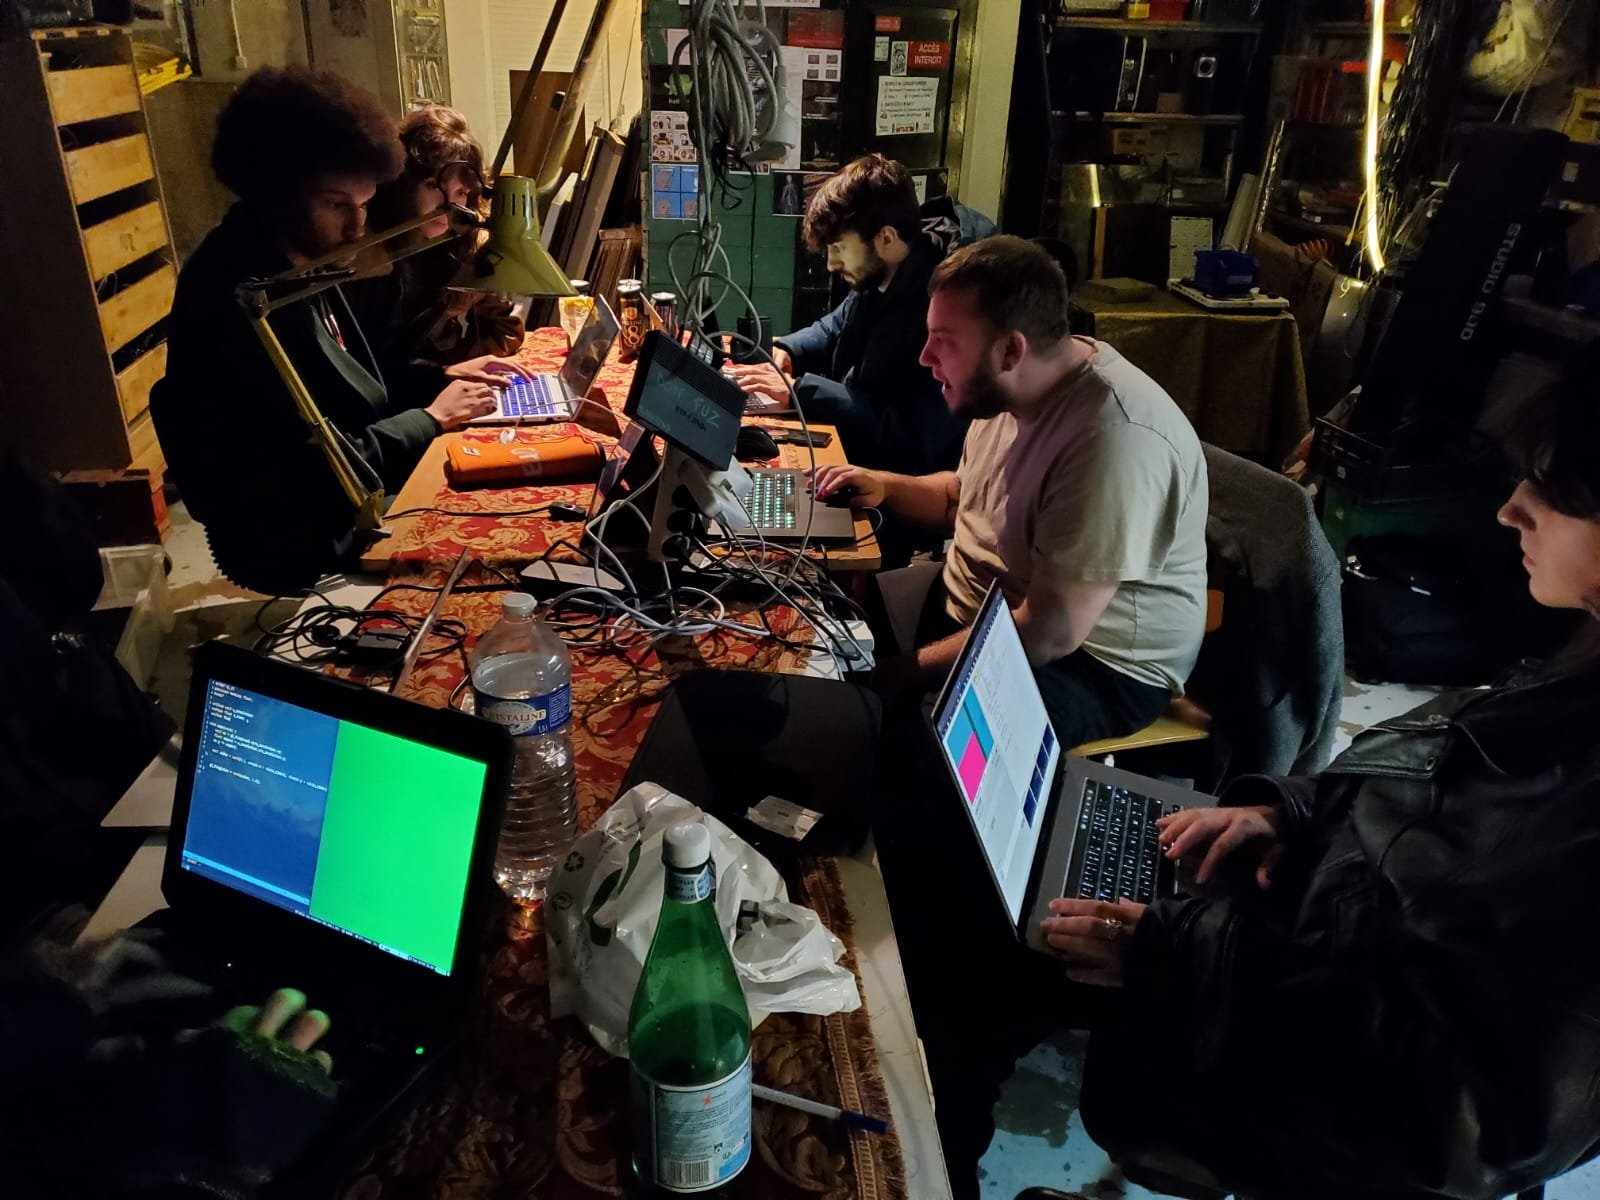
\includegraphics[width=\linewidth]{images/introduction/intro04.jpg}
    \caption{Ateliers \textit{creative coding} au Fuz (photo Léon Denise)}
    \label{intro04}
  \end{minipage}
  \hspace{0.1\linewidth} % Espace horizontal pour la gouttière
  \begin{minipage}[b]{0.45\linewidth}
    \centering
    \includegraphics[width=\linewidth]{images/introduction/intro07.png}
    \caption{Performance son / visuels (photo Émilie Corne)}
    \label{intro07}
  \end{minipage}
\end{figure}

À noter aussi qu'une certaine frustration a marqué mon parcours : le sentiment de saturation lié à l'utilisation intensive de logiciels. Pour répondre à cette frustration, j'ai décidé de m'éloigner autant que possible de ces outils, dans une volonté affirmée de sortir de ma zone de confort.

Cette expérience avec le Cookie Collective a été source d'inspiration pour moi et a réaffirmé l'importance de la liberté créative et du pouvoir du collectif. Elle a ravivé en moi l'espoir en un art novateur, capable de dépasser les limites du « cinéma » tel que nous le connaissons aujourd'hui, et d'explorer de nouvelles voies d'expression artistique. L'esprit de communauté et l'organisation autonome de ce collectif m'ont rappelé les mouvements de \textit{free parties}\footnote{Les \textit{free parties} sont des événements musicaux et culturels autonomes, souvent organisés de manière clandestine et sans autorisation officielle, caractérisés par une programmation musicale centrée sur la musique électronique \textit{underground}. Ces événements se déroulent généralement dans des lieux inhabituels ou alternatifs, tels que des entrepôts abandonnés, des champs, des forêts ou des \textit{squats}.} des années 90 qui ont eu une influence profonde sur la culture et l'esthétique numériques contemporaines.

En assistant aux performances, j'ai constaté que l'interaction entre le \textit{livecoder} de \textit{shaders} et celui de musique était artificielle. Habituellement, c'est le \textit{livecoder} des \textit{shaders} qui ajuste ses variables en fonction du son qu'il entend, permettant ainsi au visuel de suivre le rythme. Bien que cela puisse duper le public, cette observation m'a incité à rechercher un moyen d'obtenir une interaction authentique entre le son et le visuel. C'est précisément le sujet principal abordé dans ce mémoire.

Dans la première partie, je revisiterai les origines de la \textit{demoscene}, en adoptant un angle plus historique que technique. Cette démarche répond à un double objectif : enrichir ma culture personnelle et mieux comprendre cet univers pour m'y intégrer pleinement. 

La deuxième partie, précédée d'un bref rappel sur le \textit{pipeline} graphique, constitue une sorte de tutoriel visant à présenter les techniques essentielles du \textit{livecoding}. Pour des raisons de lisibilité, j'ai opté pour une décomposition en deux sections. La première traitera des techniques fondamentales pour écrire des \textit{fragment shaders} en temps réel, tandis que la seconde explorera des techniques plus avancées mais optionnelles.

Conscient que certains de mes camarades de promotion sont passionnés par le développement et la manipulation des \textit{shaders} sans nécessairement maîtriser la logique mathématique sous-jacente, j'ai cherché à rendre ces concepts accessibles et didactiques. J'espère ainsi susciter leur intérêt pour la programmation des \textit{shaders}.

Enfin, la dernière partie de ce mémoire sera consacrée à mes expérimentations, mettant en lumière certains langages spécifiques au \textit{livecoding} musical, notamment FoxDot et Orca. Ces solutions se sont avérées parfaitement adaptées à mes besoins, car FoxDot offre une expérience proche de la notation musicale traditionnelle, en rapport avec mon expérience en gravure musicale\footnote{La gravure musicale est le processus de notation ou de transcription de la musique dans un format numérique à l'aide de logiciels spécialisés. Cette pratique consiste à représenter les éléments musicaux tels que les notes, les rythmes, les indications de tempo, les dynamiques et d'autres instructions d'interprétation de manière visuelle et compréhensible pour les musiciens. Les principales solutions logicielles de gravure musicale comprennent des programmes tels que Finale, MuseScore et LilyPond (ma solution privilégiée).}, tandis qu'Orca m'a séduit par sa syntaxe originale et sa créativité graphique.

Après avoir exploré en détail la structure d'un fichier MIDI (consultable en annexe), la fin de cette dernière partie sera consacrée à l'introduction d'une solution visant à récupérer les informations MIDI en vue d'animer un \textit{shader}. Cette approche évite l'utilisation de logiciels tiers pour se rapprocher d'un \textit{pipeline} de développement purement basé sur le code.

Il me semblait aussi important de souligner que mon intention première était d'inclure des chapitres dédiés à l'\textit{algorave} et à la musique algorithmique. Cependant, en raison d'une contrainte de temps et d'une surestimation de mes capacités, j'ai été contraint d'abandonner ces sujets.

\newpage


\begin{figure}[htbp]
  \begin{minipage}[b]{0.45\linewidth}
    \centering
    \includegraphics[width=\linewidth]{images/introduction/intro06.png}
    \caption{Performance musique/\textit{shaders} (photo Émilie Corne)}
    \label{intro06}
  \end{minipage}
  \hspace{0.1\linewidth} % Espace horizontal pour la gouttière
  \begin{minipage}[b]{0.45\linewidth}
    \centering
    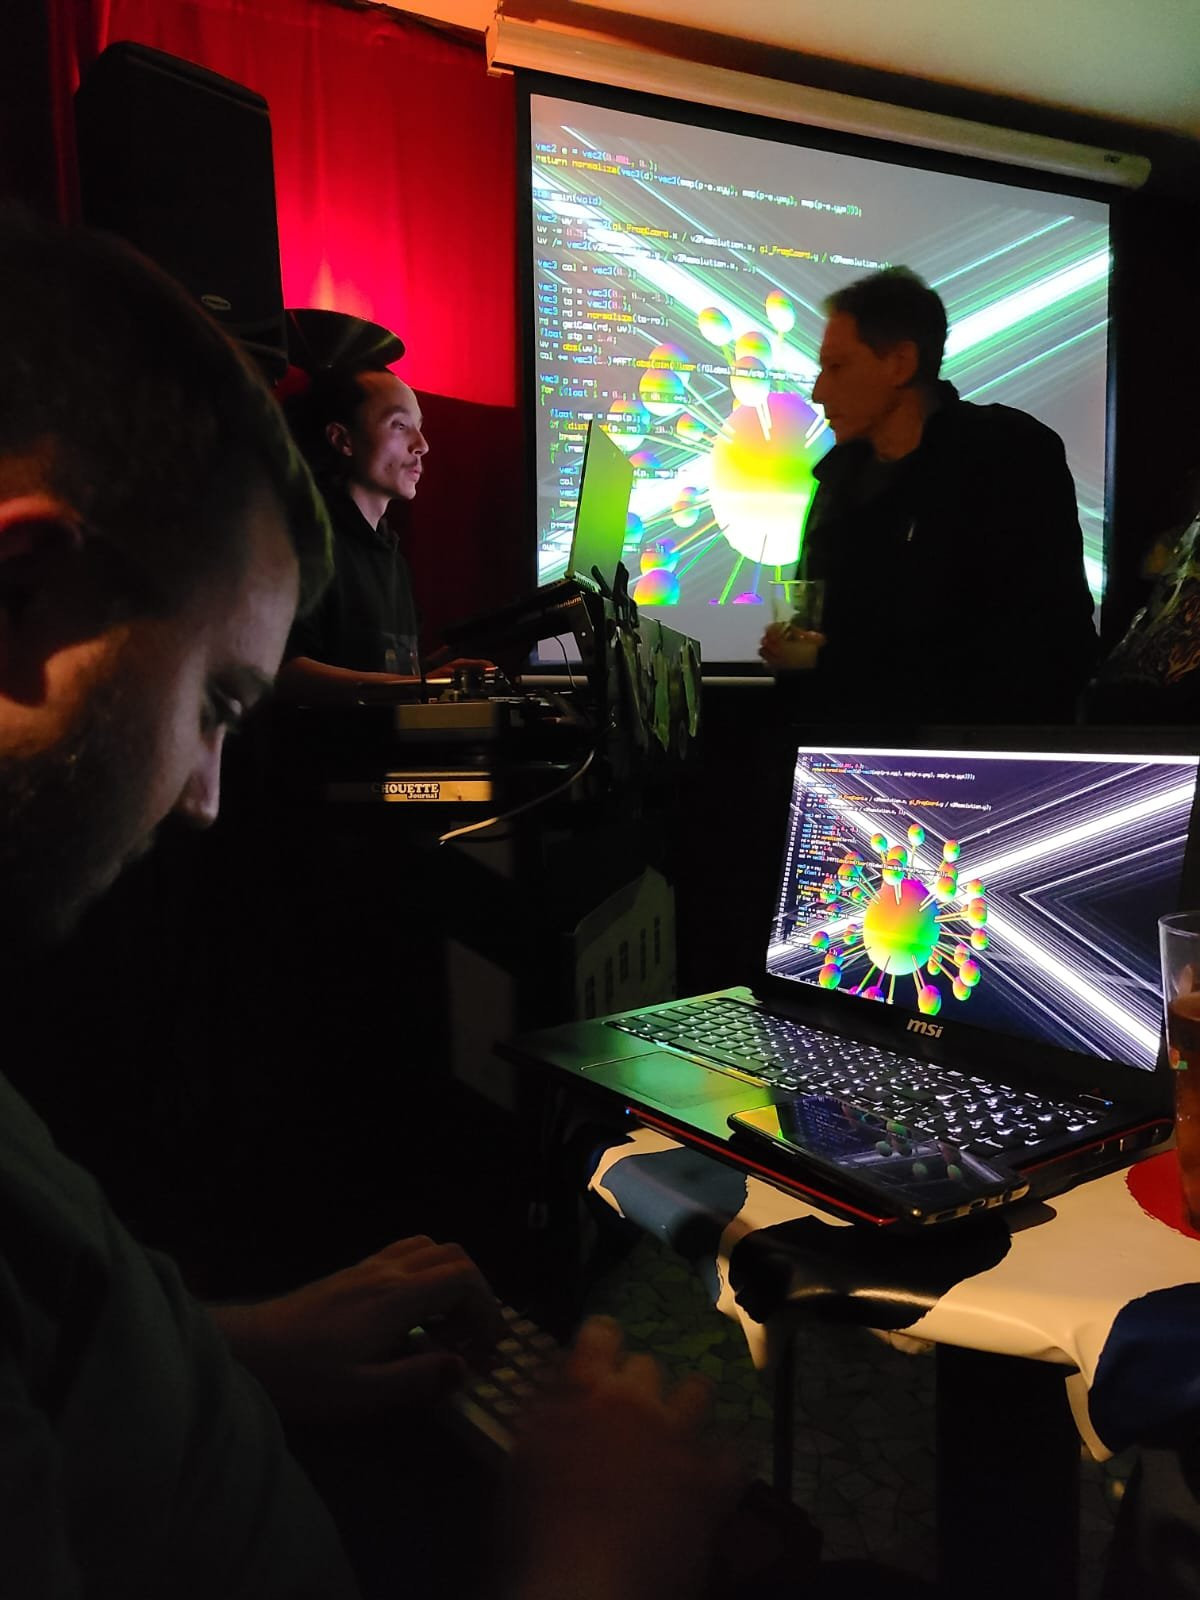
\includegraphics[width=\linewidth]{images/introduction/intro02.jpg}
    \caption{Performance musique/\textit{shaders} au bar la Chair de Poule (photo Léon Denise)}
    \label{intro02}
  \end{minipage}
\end{figure}

% **DEMOSCENE**
% **La demoscne**
\chapter{\textit{Demoscene}: origine et évolution}
\setlength{\epigraphwidth}{0.7\linewidth} % Ajustez la largeur selon vos besoins
% \todo{vérifier largeur epigraph flopine}

\epigraph{Au sein de la riche mosaïque de la culture urbaine, une multitude de formes d'expression personnelle émergent et trouvent leur voie. Qu'il s'agisse de pensées, d'images, de rythmes et mélodies, ou même de parfums et matériaux transformés, tout devient prétexte à traduire une émotion humaine. Mais que se produit-il lorsque quelqu'un choisit de 
communiquer par le biais des nombres ?}{\textit{Moleman 2 - Demoscene - The Art of the Algorithms (2012) - Documentaire}}

% Livre Freaks\cite{polgarFreaxBriefHistory2016}


\section{Préambule}

En guise de préambule, il me semblait important de mentionner que les illustrations de ce chapitre sont des \textit{strips}\footnote{Un \textit{strip} désigne généralement une bande d'images ou de vignettes disposées dans un ordre séquentiel, souvent utilisée dans le contexte des bandes dessinées.} représentant trois images d'une \textit{demo}, disposées dans l'ordre chronologique de la \textit{demo} elle-même. Ces images ont été extraites des sites \href{https://pouet.net}{pouet.net} et \href{https://demozoo.org}{demozoo.org}. Leur insertion vise à aérer la lecture de ce premier chapitre et à fournir des exemples visuels pour illustrer certains effets ou concepts discutés dans le texte. L'ordre dans lequel la grande majorité de ces \textit{strips} apparaissent au sein du texte est totalement aléatoire, sans aucune notion de chronologie.

% origines de la \textit{demoscene}
% \newpage
\section{Introduction à la \textit{demo}}
\begin{figure}[h]
  \begin{minipage}[b]{0.30\linewidth}
    \centering
    
\includegraphics[width=\linewidth]{images/demoscene/demos/kewl1.png}
  \end{minipage}
  \hfill
  \begin{minipage}[b]{0.30\linewidth}
    \centering
    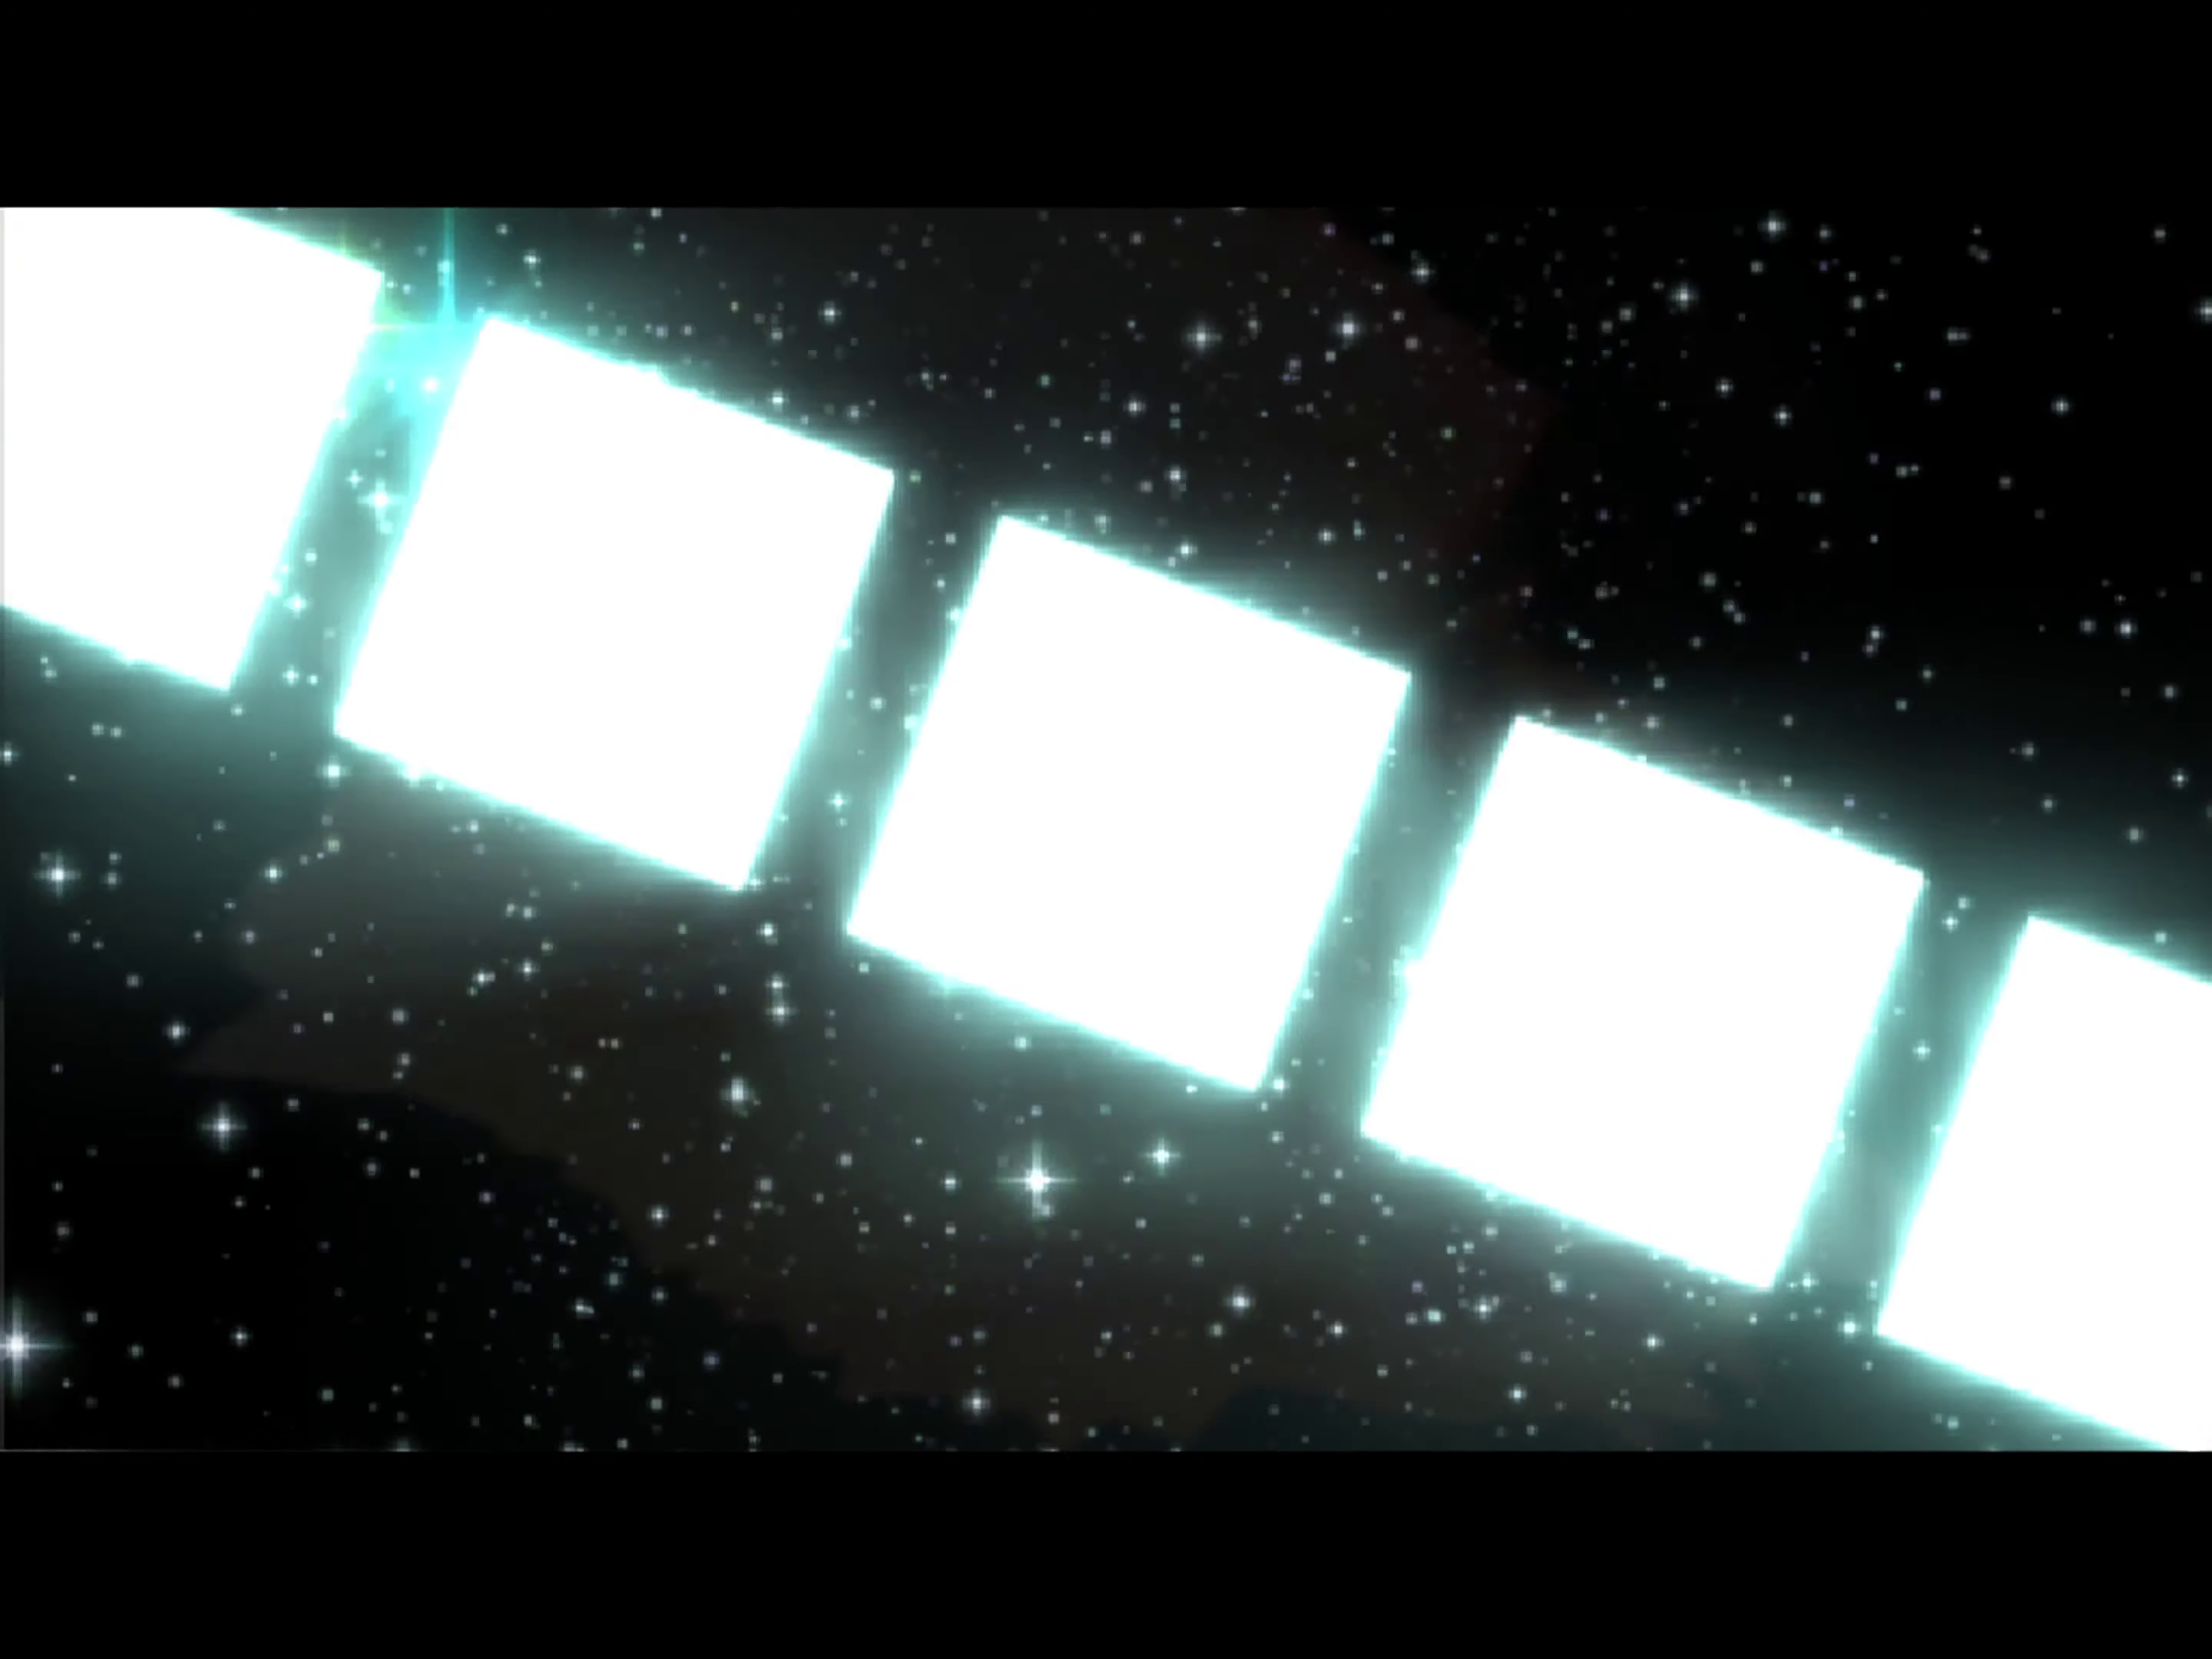
\includegraphics[width=\linewidth]{images/demoscene/demos/kewl2.png}
  \end{minipage}
  \hfill
  \begin{minipage}[b]{0.30\linewidth}
    \centering
    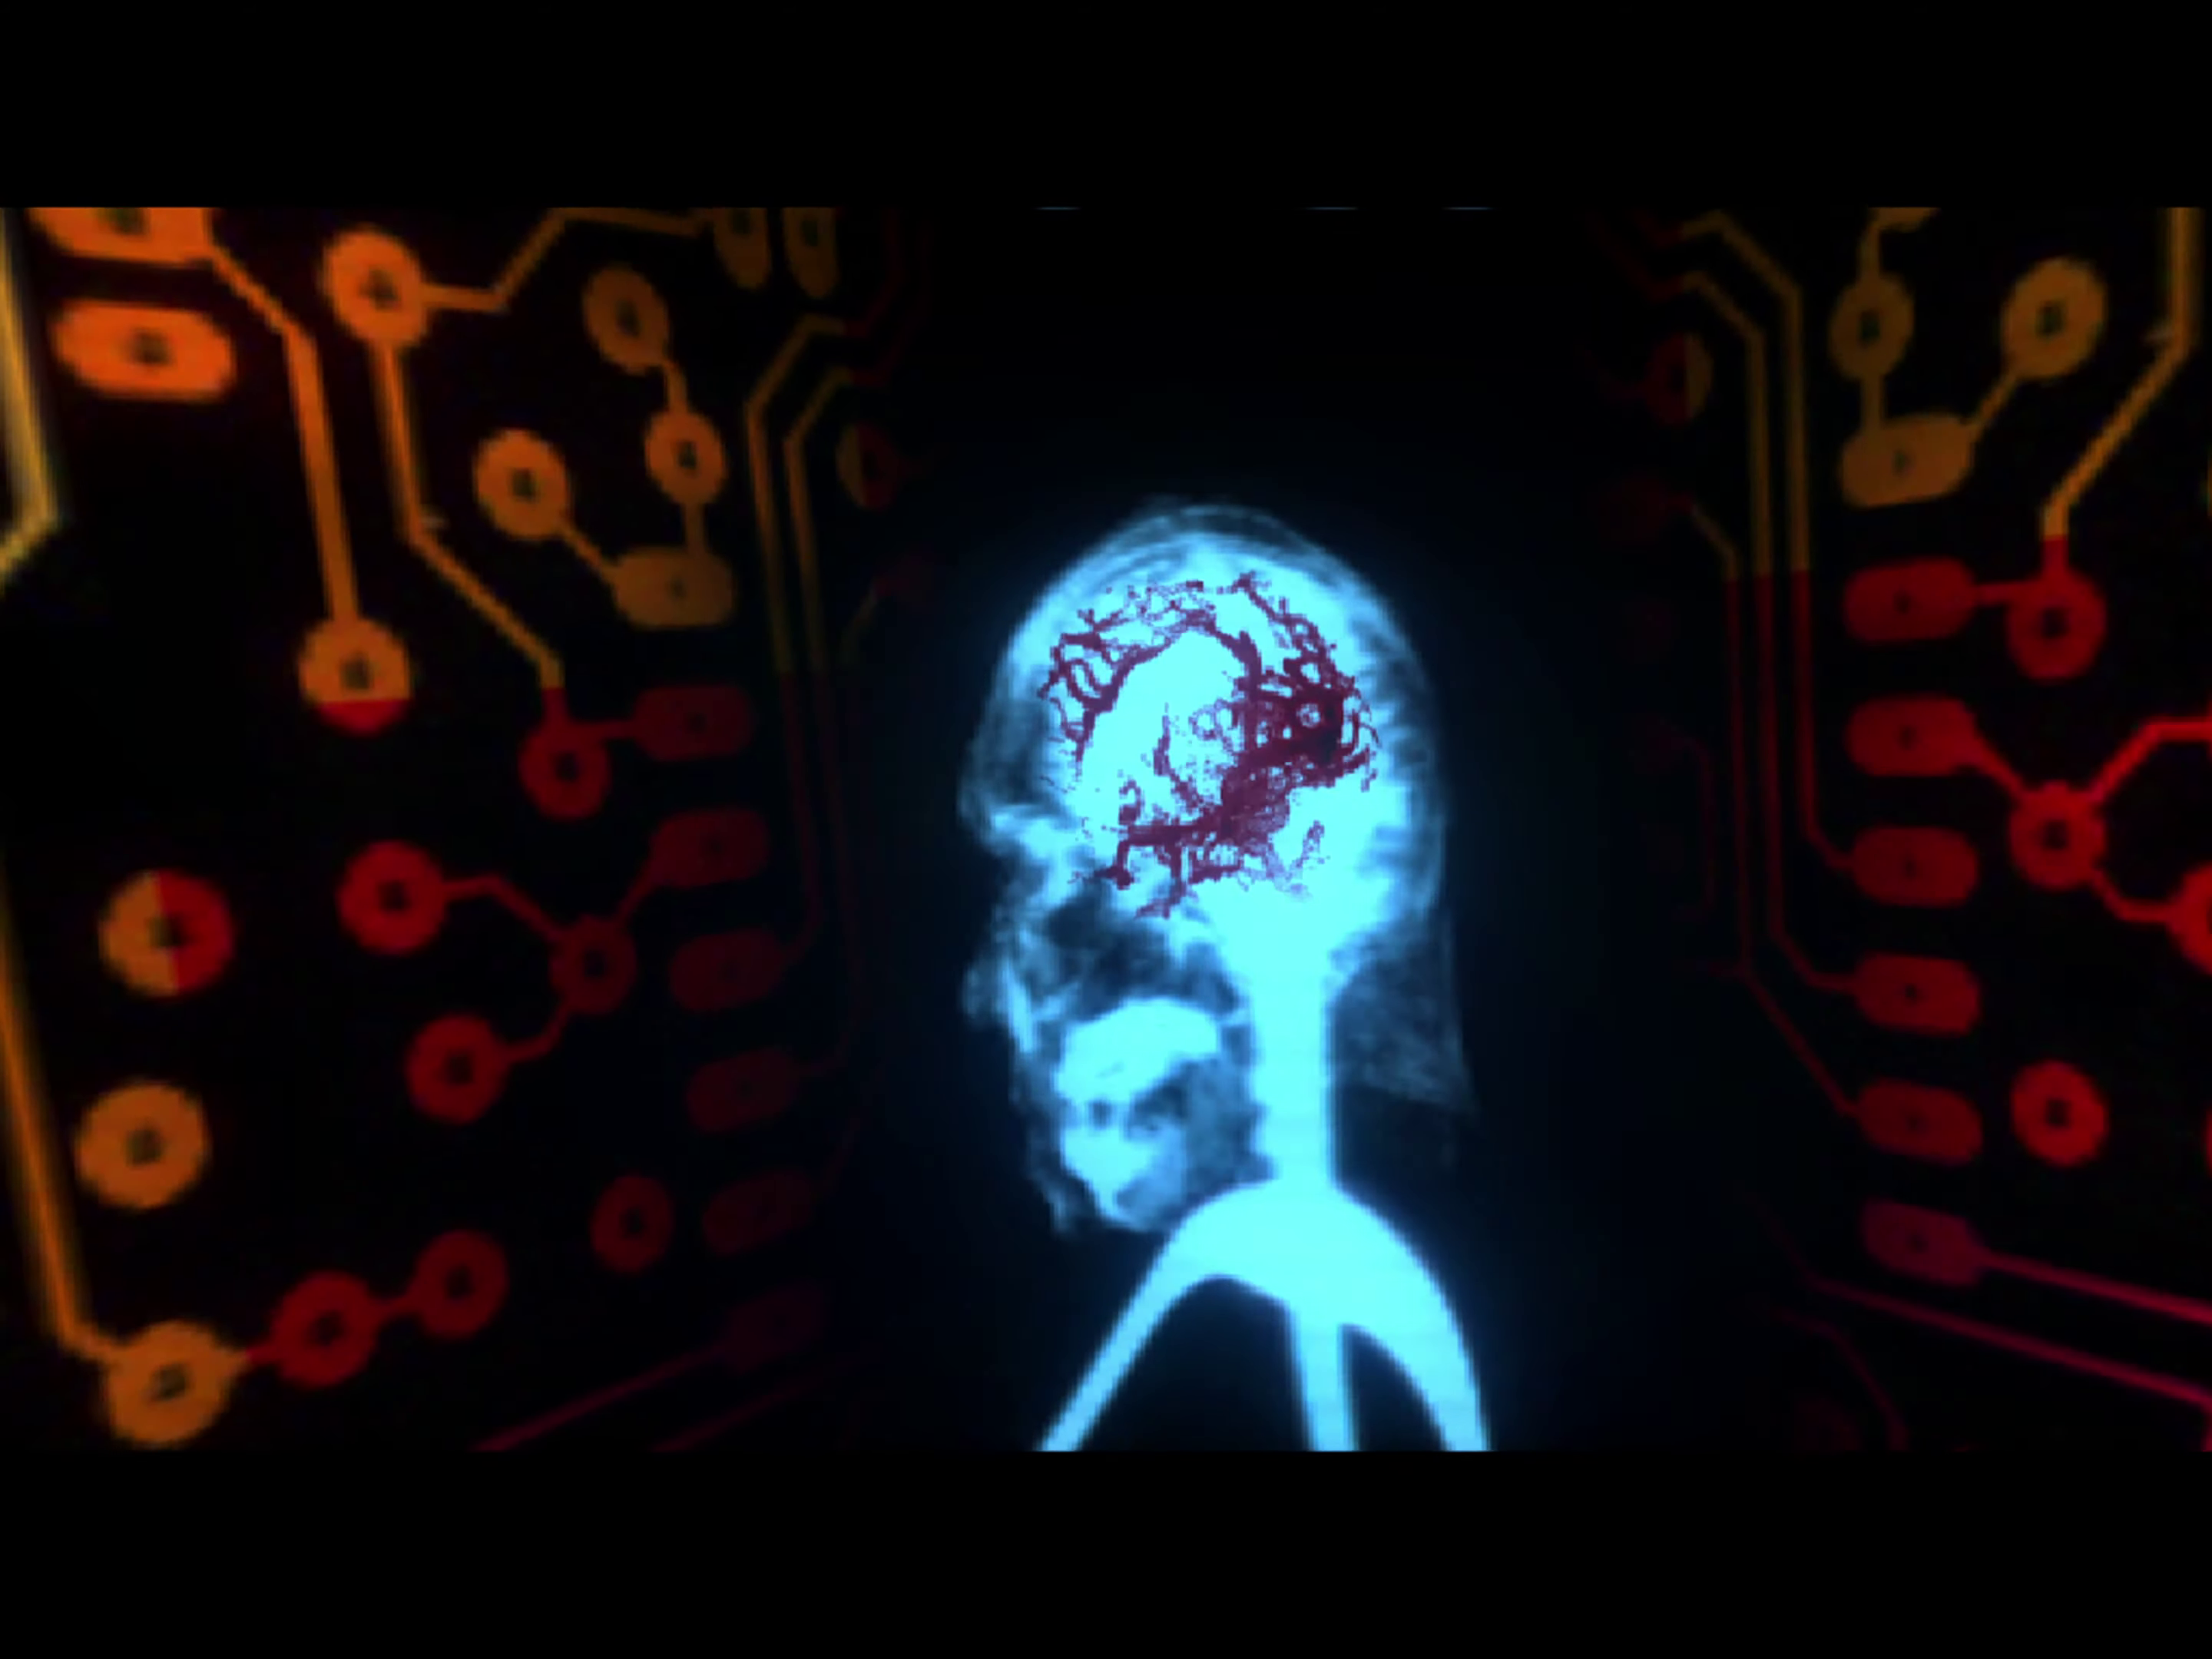
\includegraphics[width=\linewidth]{images/demoscene/demos/kewl3.png}
  \end{minipage}
  \caption{Kewlers - 1995}
  \label{kewl}
\end{figure}

\subsection*{La dualité du terme \textit{demo} dans la \textit{demoscene}}




Le terme \textit{demo} peut évoquer pour certains les démos de jeux vidéo. Cependant, au sein de la \textit{demoscene}, sa signification s'écarte sensiblement de cette conception. Alors qu'une démo de jeu est conçue pour présenter un aperçu restreint du produit final, une \textit{demo} dans le contexte de la \textit{demoscene} se présente comme une œuvre d'art autonome, élaborée pour explorer et repousser les frontières techniques et esthétiques d'un système informatique.






Si les \textit{demos} et les jeux vidéo partagent des techniques et des compétences techniques avancées, leurs aspirations divergent nettement. Alors que les jeux vidéo adhèrent généralement à un scénario préétabli, une \textit{demo} cherche à transcender les contraintes techniques pour offrir une expérience sensorielle riche, souvent assimilée à un clip musical.



\subsection*{La \textit{demo} : entre performance et exécutable}




Pour appréhender pleinement la notion de \textit{demo}, il convient de se pencher sur son étymologie anglaise, \textit{demonstration}, qui suggère une performance visant à captiver et impressionner l'auditoire. Conceptuellement, une \textit{demo} peut être comparée à une animation musicale d'une durée généralement restreinte, souvent quelques minutes. Toutefois, elle ne se réduit ni à une simple vidéo ni à un fichier audio. En réalité, une \textit{demo} est un programme exécutable, un fichier binaire, au même titre qu'un logiciel ou un jeu vidéo traditionnel.

\subsection*{Repousser les limites techniques des \textit{demos}}

Pour dépasser ces contraintes techniques, les programmeurs de \textit{demos} doivent optimiser leur code afin de produire des effets visuels tout en utilisant un minimum de ressources. Nombreux sont les \textit{demosceners} en quête de techniques permettant d'afficher des graphismes spectaculaires et de repousser les limites de ce qui est réalisable sur une plateforme spécifique.

\subsection*{La vitalité de la \textit{demoscene} en Allemagne et dans les pays scandinaves}




Il est important de souligner que la \textit{demoscene} trouve son épicentre de vitalité et de succès en Allemagne et dans les pays scandinaves, où elle jouit d'une forte implantation et d'une activité soutenue. Cette prééminence régionale s'explique en partie par la longue tradition de ces pays dans la mise en avant des compétences en informatique et en art numérique.

Ces nations sont également le berceau des plus grandes \textit{demoparties} annuelles. Par exemple, la Breakpoint en Allemagne, qui a eu lieu huit fois jusqu'en 2010, attirait régulièrement une audience dépassant le millier de visiteurs venus de près de trente nations différentes. Des événements similaires, tels que l'Assembly en Finlande ou The Gathering en Norvège, bien qu'initialement axés sur la mise en avant des compétences artistiques et informatiques, ont également élargi leur public pour inclure les passionnés de jeux sur PC. Malgré la tenue d'événements plus modestes à travers le monde, le nombre total de productions dévoilées lors de ces rassemblements dépasse désormais les 50 000. 




\subsection*{Reconnaissance internationale de la \textit{demoscene} par l'UNESCO}

En 2020, la Finlande a inscrit la \textit{demoscene} sur sa liste nationale du patrimoine culturel immatériel de l'UNESCO\footnote{Le
 patrimoine culturel immatériel, selon l'UNESCO, se réfère aux 
pratiques, représentations, expressions, connaissances et savoir-faire -
 ainsi que les instruments, objets, artefacts et espaces culturels 
associés - que les communautés, les groupes et, dans certains cas, les 
individus reconnaissent comme faisant partie de leur patrimoine 
culturel.}, marquant ainsi une reconnaissance significative de cette forme d'expression artistique numérique. Cette démarche a fait de la \textit{demoscene} la première sous-culture numérique à être honorée sur une liste de patrimoine culturel immatériel de l'UNESCO. Plus tard, en 2021, l'Allemagne et la Pologne ont également suivi en 
ajoutant la \textit{demoscene} à leur liste nationale du patrimoine culturel immatériel de l'UNESCO, suivies par les Pays-Bas en 2023.
% origines de la \textit{demoscene}

\newpage
\section{Origines de la \textit{demoscene}}
\begin{figure}[h]
  \begin{minipage}[b]{0.30\linewidth}
    \centering
    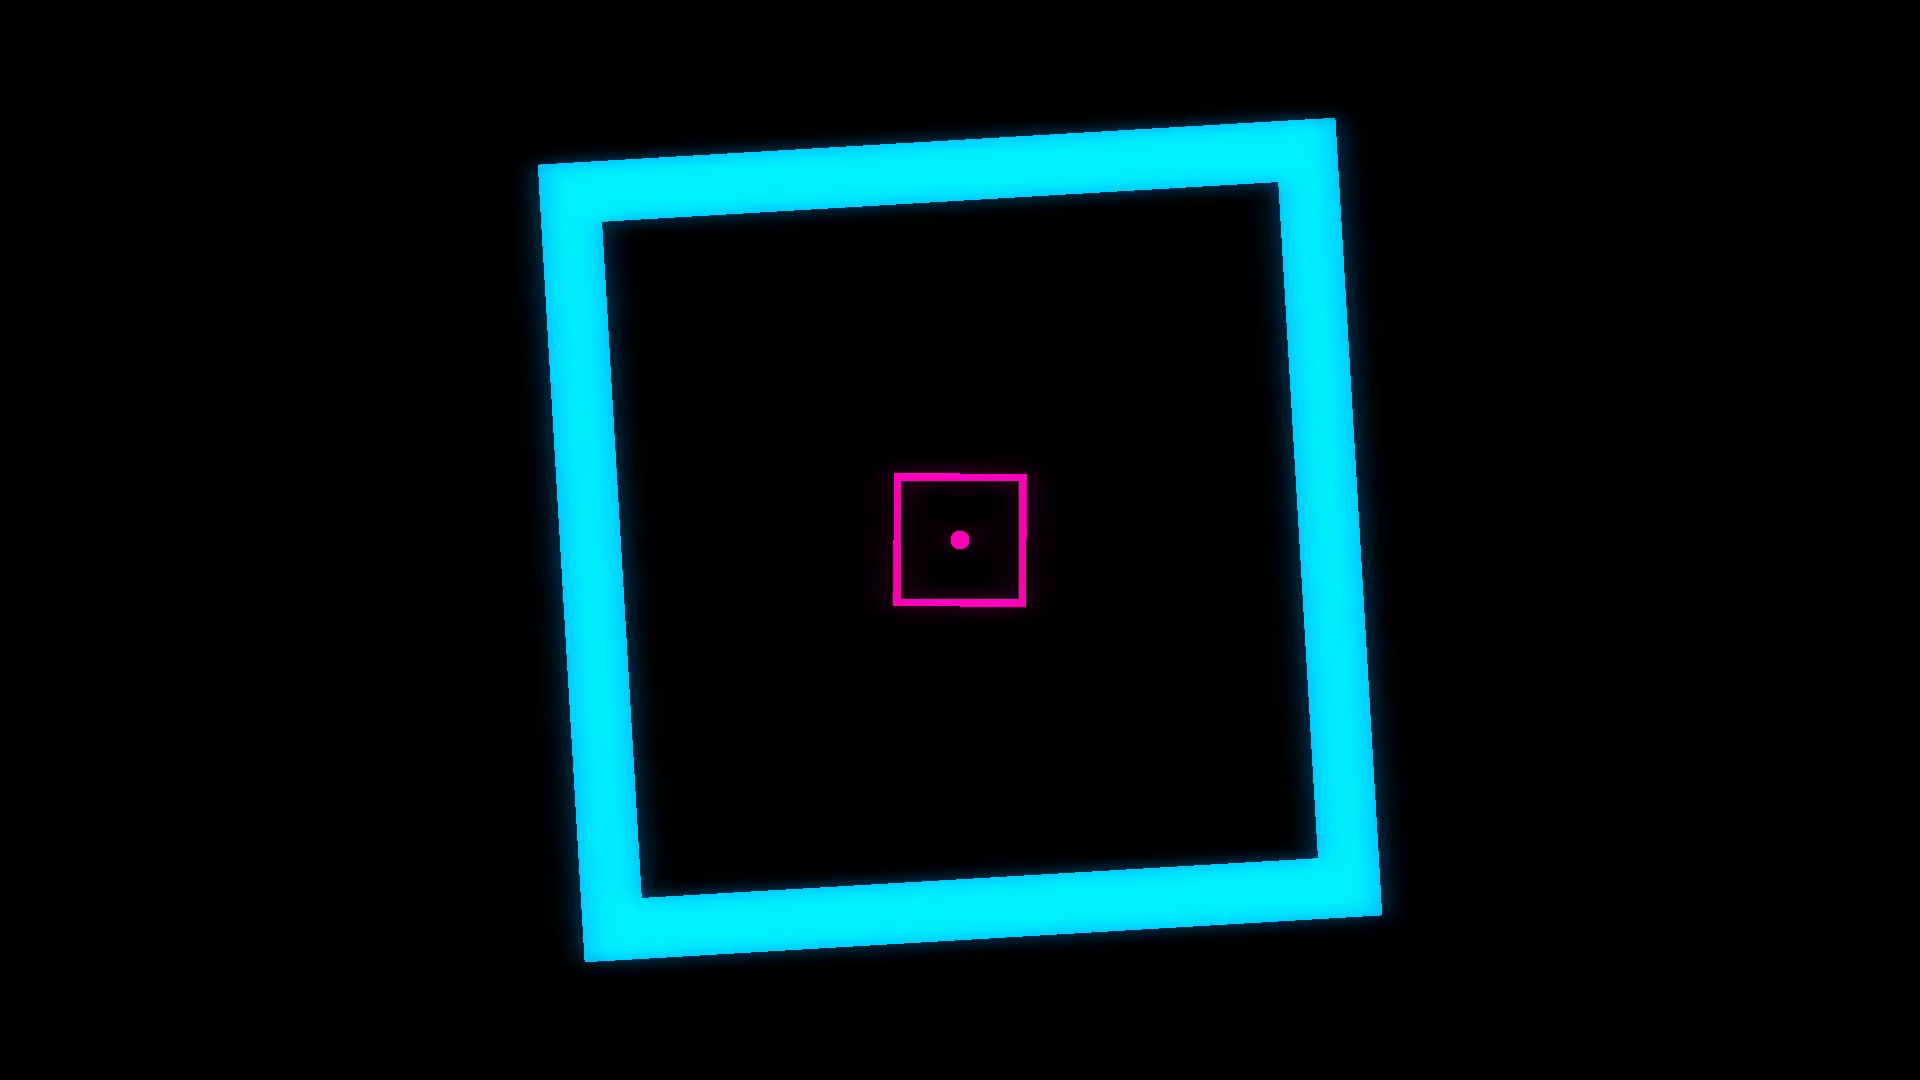
\includegraphics[width=\linewidth]{images/demoscene/demos/ninja1.png}
  \end{minipage}
  \hfill
  \begin{minipage}[b]{0.30\linewidth}
    \centering
    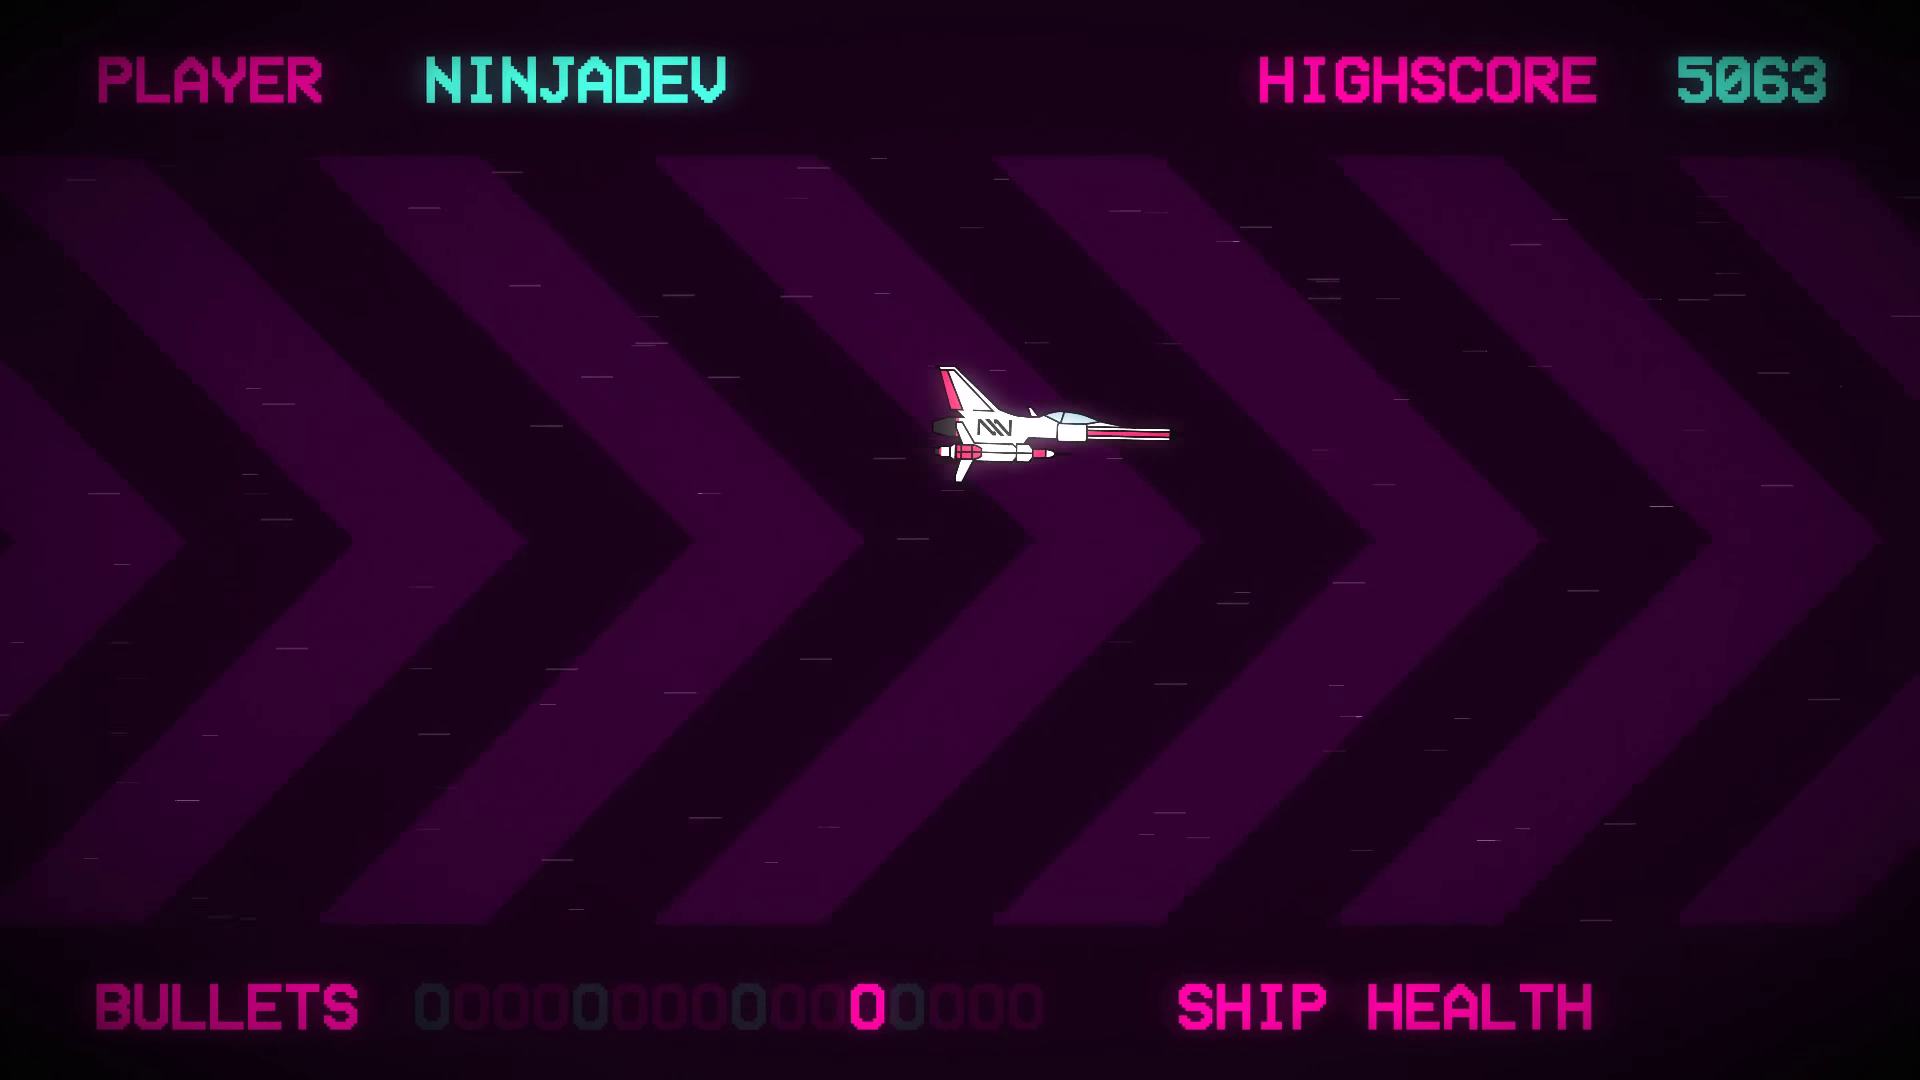
\includegraphics[width=\linewidth]{images/demoscene/demos/ninja2.png}
  \end{minipage}
  \hfill
  \begin{minipage}[b]{0.30\linewidth}
    \centering
    
\includegraphics[width=\linewidth]{images/demoscene/demos/ninja3.png}
  \end{minipage}
  \caption{Ninjadev – What Are You Syncing About?}
  \label{ninja}
\end{figure}




\subsection*{L'impact du Commodore 64 sur l'émergence de la \textit{demoscene}}


On peut situer les origines des \textit{demos} autour des années 1983-1984, marquées par l'introduction du Commodore 64 (C64) en 1982. Le Commodore 64  est un ordinateur personnel qui a rapidement conquis le marché grâce à son prix attractif et à sa vaste ludothèque. À cette époque, il rivalisait avec les bornes d'arcade en termes de qualité sonore et graphique, éclipsant les consoles de jeux non programmables. Sur le plan matériel, le C64 disposait d'un microprocesseur MOS Technology 6510 à 1 MHz, de 64 Ko de mémoire RAM\footnote{La RAM (\textit{Random Access Memory}) est une forme de mémoire volatile utilisée par les ordinateurs pour stocker des données temporaires qui peuvent être rapidement lues et écrites par le processeur et d'autres périphériques.} (d'où son nom), et d'une puce graphique et sonore intégrée, le SID (\textit{Sound Interface Device}) (voir \ref{Commodore64_00} et \ref{Commodore64_01}). Cette dernière offrait des capacités graphiques et sonores avancées pour son époque.

\begin{figure}[h]
  \begin{minipage}[b]{0.40\linewidth}
    \centering
    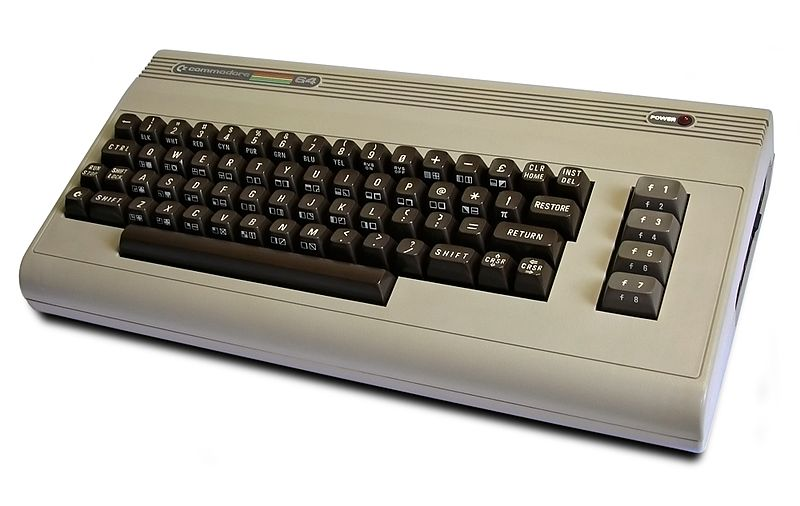
\includegraphics[width=\linewidth, height=1.5in]{images/demoscene/Commodore64_00.jpg}
    \caption{Commodore 64}
    \label{Commodore64_00}
  \end{minipage}
  \hspace{0.1\linewidth} % Espace horizontal pour la gouttière
  \begin{minipage}[b]{0.40\linewidth}
    \centering
    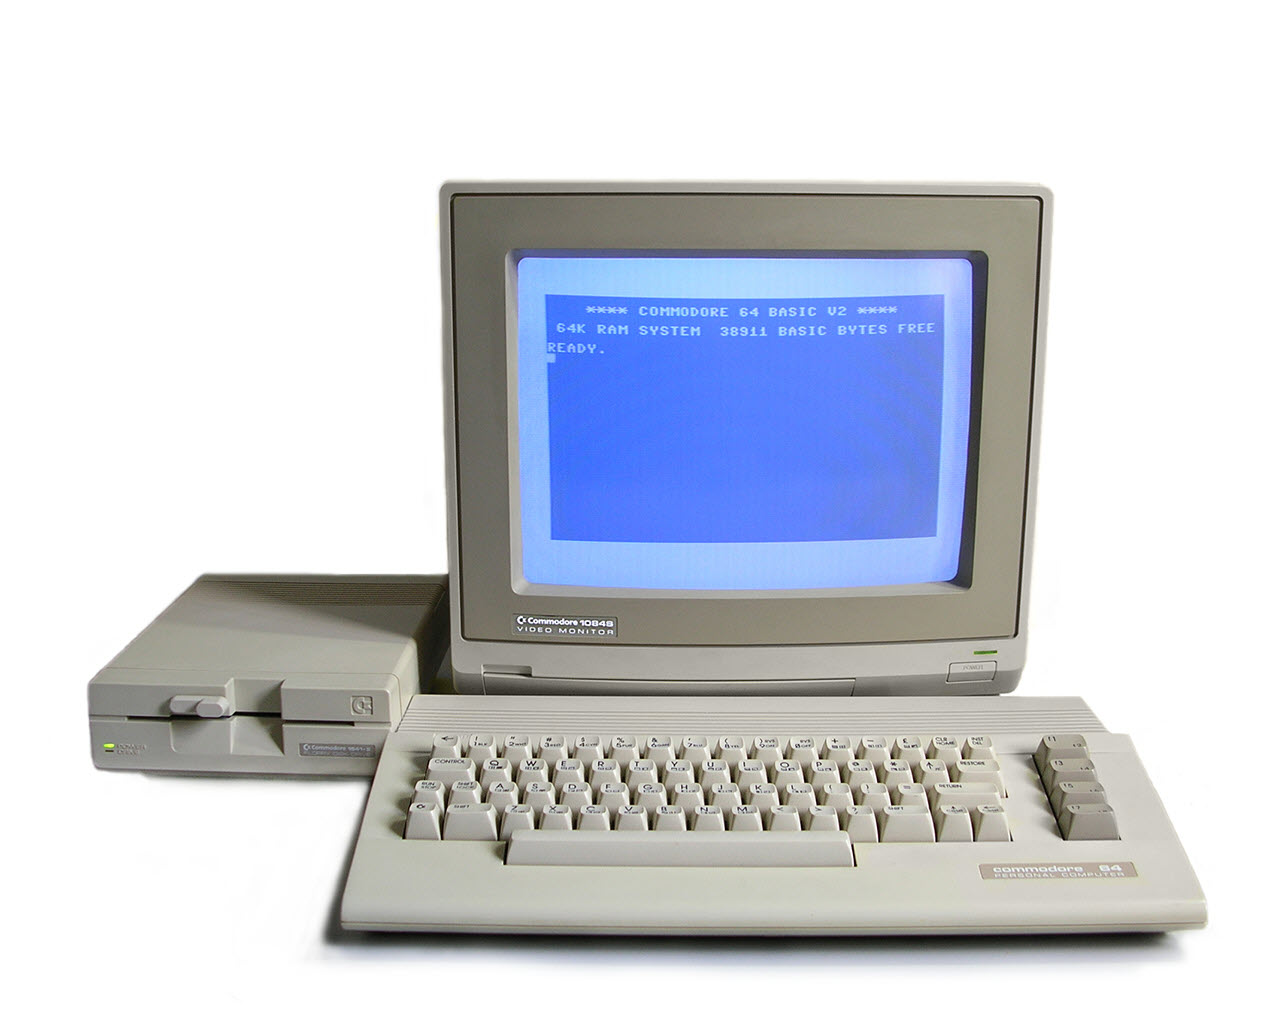
\includegraphics[width=\linewidth, height=1.5in]{images/demoscene/Commodore64_01.jpg}
    \caption{Commodore 64 avec écran et lecteur de disquette}
    \label{Commodore64_01}
  \end{minipage}
\end{figure}


Le Commodore 64 a grandement contribué à populariser l'informatique personnelle et a été un acteur clé dans l'émergence de la culture \textit{hacker}, de la \textit{demoscene}, et de l'industrie du jeu vidéo telle qu'elle est aujourd'hui.

\subsection*{Lien entre la \textit{demoscene} et l'industrie des jeux vidéo}

L'émergence et la montée en popularité de la \textit{demoscene} sont étroitement liées à l'essor des jeux vidéo. Dans les années 80, l'achat de jeux vidéo était souvent une décision risquée en raison de leur coût élevé et de l'absence de critiques ou de journalisme spécialisé pour guider les consommateurs. Sans avis ou évaluations disponibles, les joueurs se retrouvaient parfois déçus par la qualité des jeux qu'ils avaient achetés, découvrant des titres aux graphismes médiocres ou aux bugs gênants.




La copie de jeux est devenue alors une pratique courante, d'autant plus facilitée par la nature des supports utilisés par le Commodore 64. Contrairement aux jeux sur consoles, les jeux du C64, souvent distribués sur cassette, étaient facilement dupliquables sans perte de qualité ou d'informations.

\subsection*{Naissance des \textit{cracktros}}

\begin{figure}[h]
  \begin{minipage}[b]{0.30\linewidth}
    \centering
    
\includegraphics[width=\linewidth]{images/demoscene/demos/sani1.png}
  \end{minipage}
  \hfill
  \begin{minipage}[b]{0.30\linewidth}
    \centering
    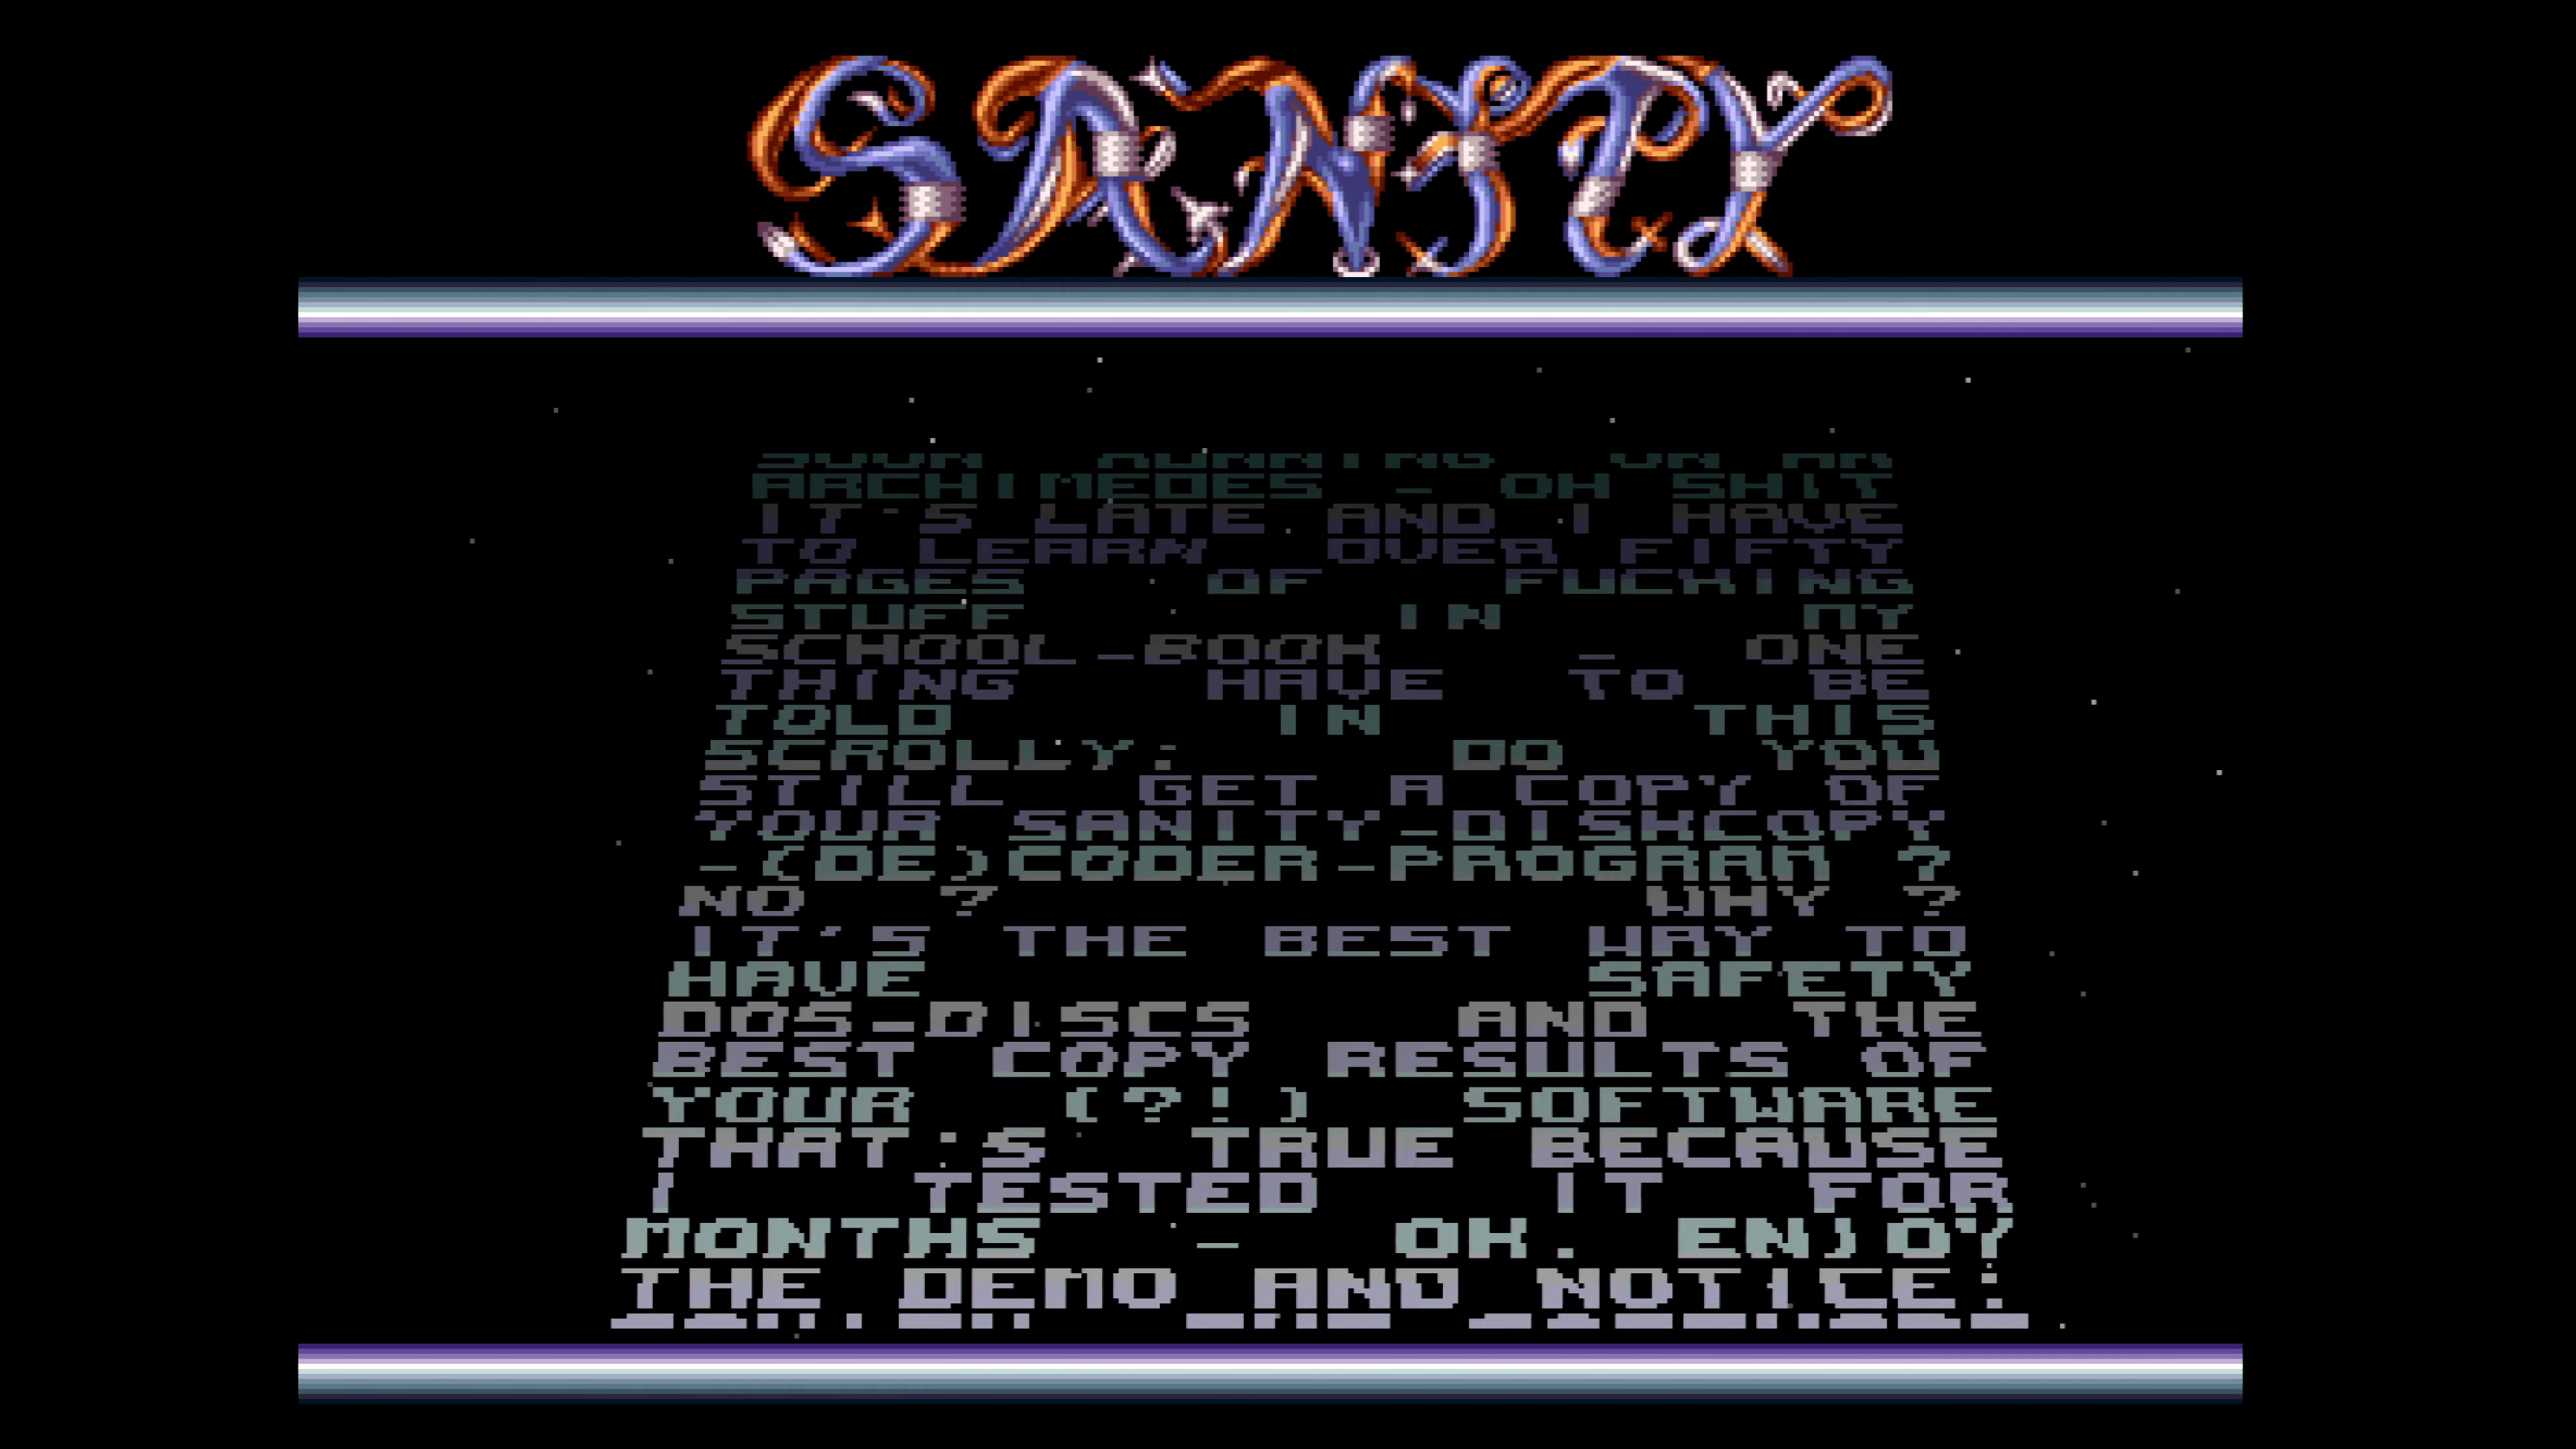
\includegraphics[width=\linewidth]{images/demoscene/demos/sani2.png}
  \end{minipage}
  \hfill
  \begin{minipage}[b]{0.30\linewidth}
    \centering
    
\includegraphics[width=\linewidth]{images/demoscene/demos/sani3.png}
  \end{minipage}
  \caption{Sanity - Elysium}
  \label{sanity}
\end{figure}


Les jeux piratés circulaient largement, échangés pendant les cours d'école ou via courrier postal. Chaque copie comportait une introduction spécifique, créée par le \textit{cracker}\footnote{Le terme \textit{cracker} désigne une personne spécialisée dans la suppression ou la contournement des protections de logiciels, principalement pour les jeux vidéo ou les applications.} responsable du piratage. Leur maîtrise de la programmation leur a permis de repousser les limites du Commodore 64. Plutôt que d'utiliser le langage BASIC, plus lent, les \textit{crackers} se sont tournés vers l'assembleur, un langage de bas niveau permettant d'optimiser le code et d'accélérer considérablement l'exécution des programmes. Cette approche leur permettait d'obtenir des performances jusqu'à 30 fois supérieures, transformant ainsi la manière dont les jeux étaient perçus et joués sur le Commodore 64. Ils ont également expérimenté les capacités du C64 pour créer des images et des sons, créant ainsi des expériences audiovisuelles immersives. En utilisant le langage des mathématiques pour coder des programmes, ils ont ouvert la voie à l'expression artistique numérique.

En plus de rendre les jeux gratuits, les \textit{crackers} offraient des avantages tels que des vies infinies ou la suppression d'ennemis, permettant ainsi aux joueurs d'éviter les obstacles frustrants et de profiter pleinement de leur expérience de jeu. Fiers de leurs exploits, ces \textit{crackers} intégraient fréquemment leurs initiales ou le nom de leur groupe au démarrage des jeux, que ce soit dans une liste de meilleurs scores ou à travers des éléments graphiques. Ces ajouts servaient de vitrine à leur talent et renforçaient l'identité de leur groupe au sein de la communauté.

Ces introductions élaborées par les \textit{crackers} pour mettre en avant leur talent et leur travail de contournement des mesures de protection des jeux sont nommées \textit{cracktros}\footnote{Un \textit{cracktro} est une courte animation ou introduction visuelle qui apparaît avant le lancement d'un jeu vidéo ou d'un logiciel piraté.} (la contraction des mots \textit{intro} et \textit{crack}). Le \textit{cracking} est devenu bien plus qu'une simple pratique de contournement : c'était une démonstration de compétence et d'expertise technique. Ces \textit{crackers} étaient admirés au sein de la communauté pour leur capacité à maîtriser la machine et à offrir des versions optimisées des jeux. Au fil des années, ces \textit{cracktros} ont évolué pour devenir de véritables œuvres d'art numérique, gagnant en sophistication et en complexité.

\subsection*{Les groupes pionniers du \textit{cracking}}
\begin{figure}[h]
  \begin{minipage}[b]{0.30\linewidth}
    \centering
    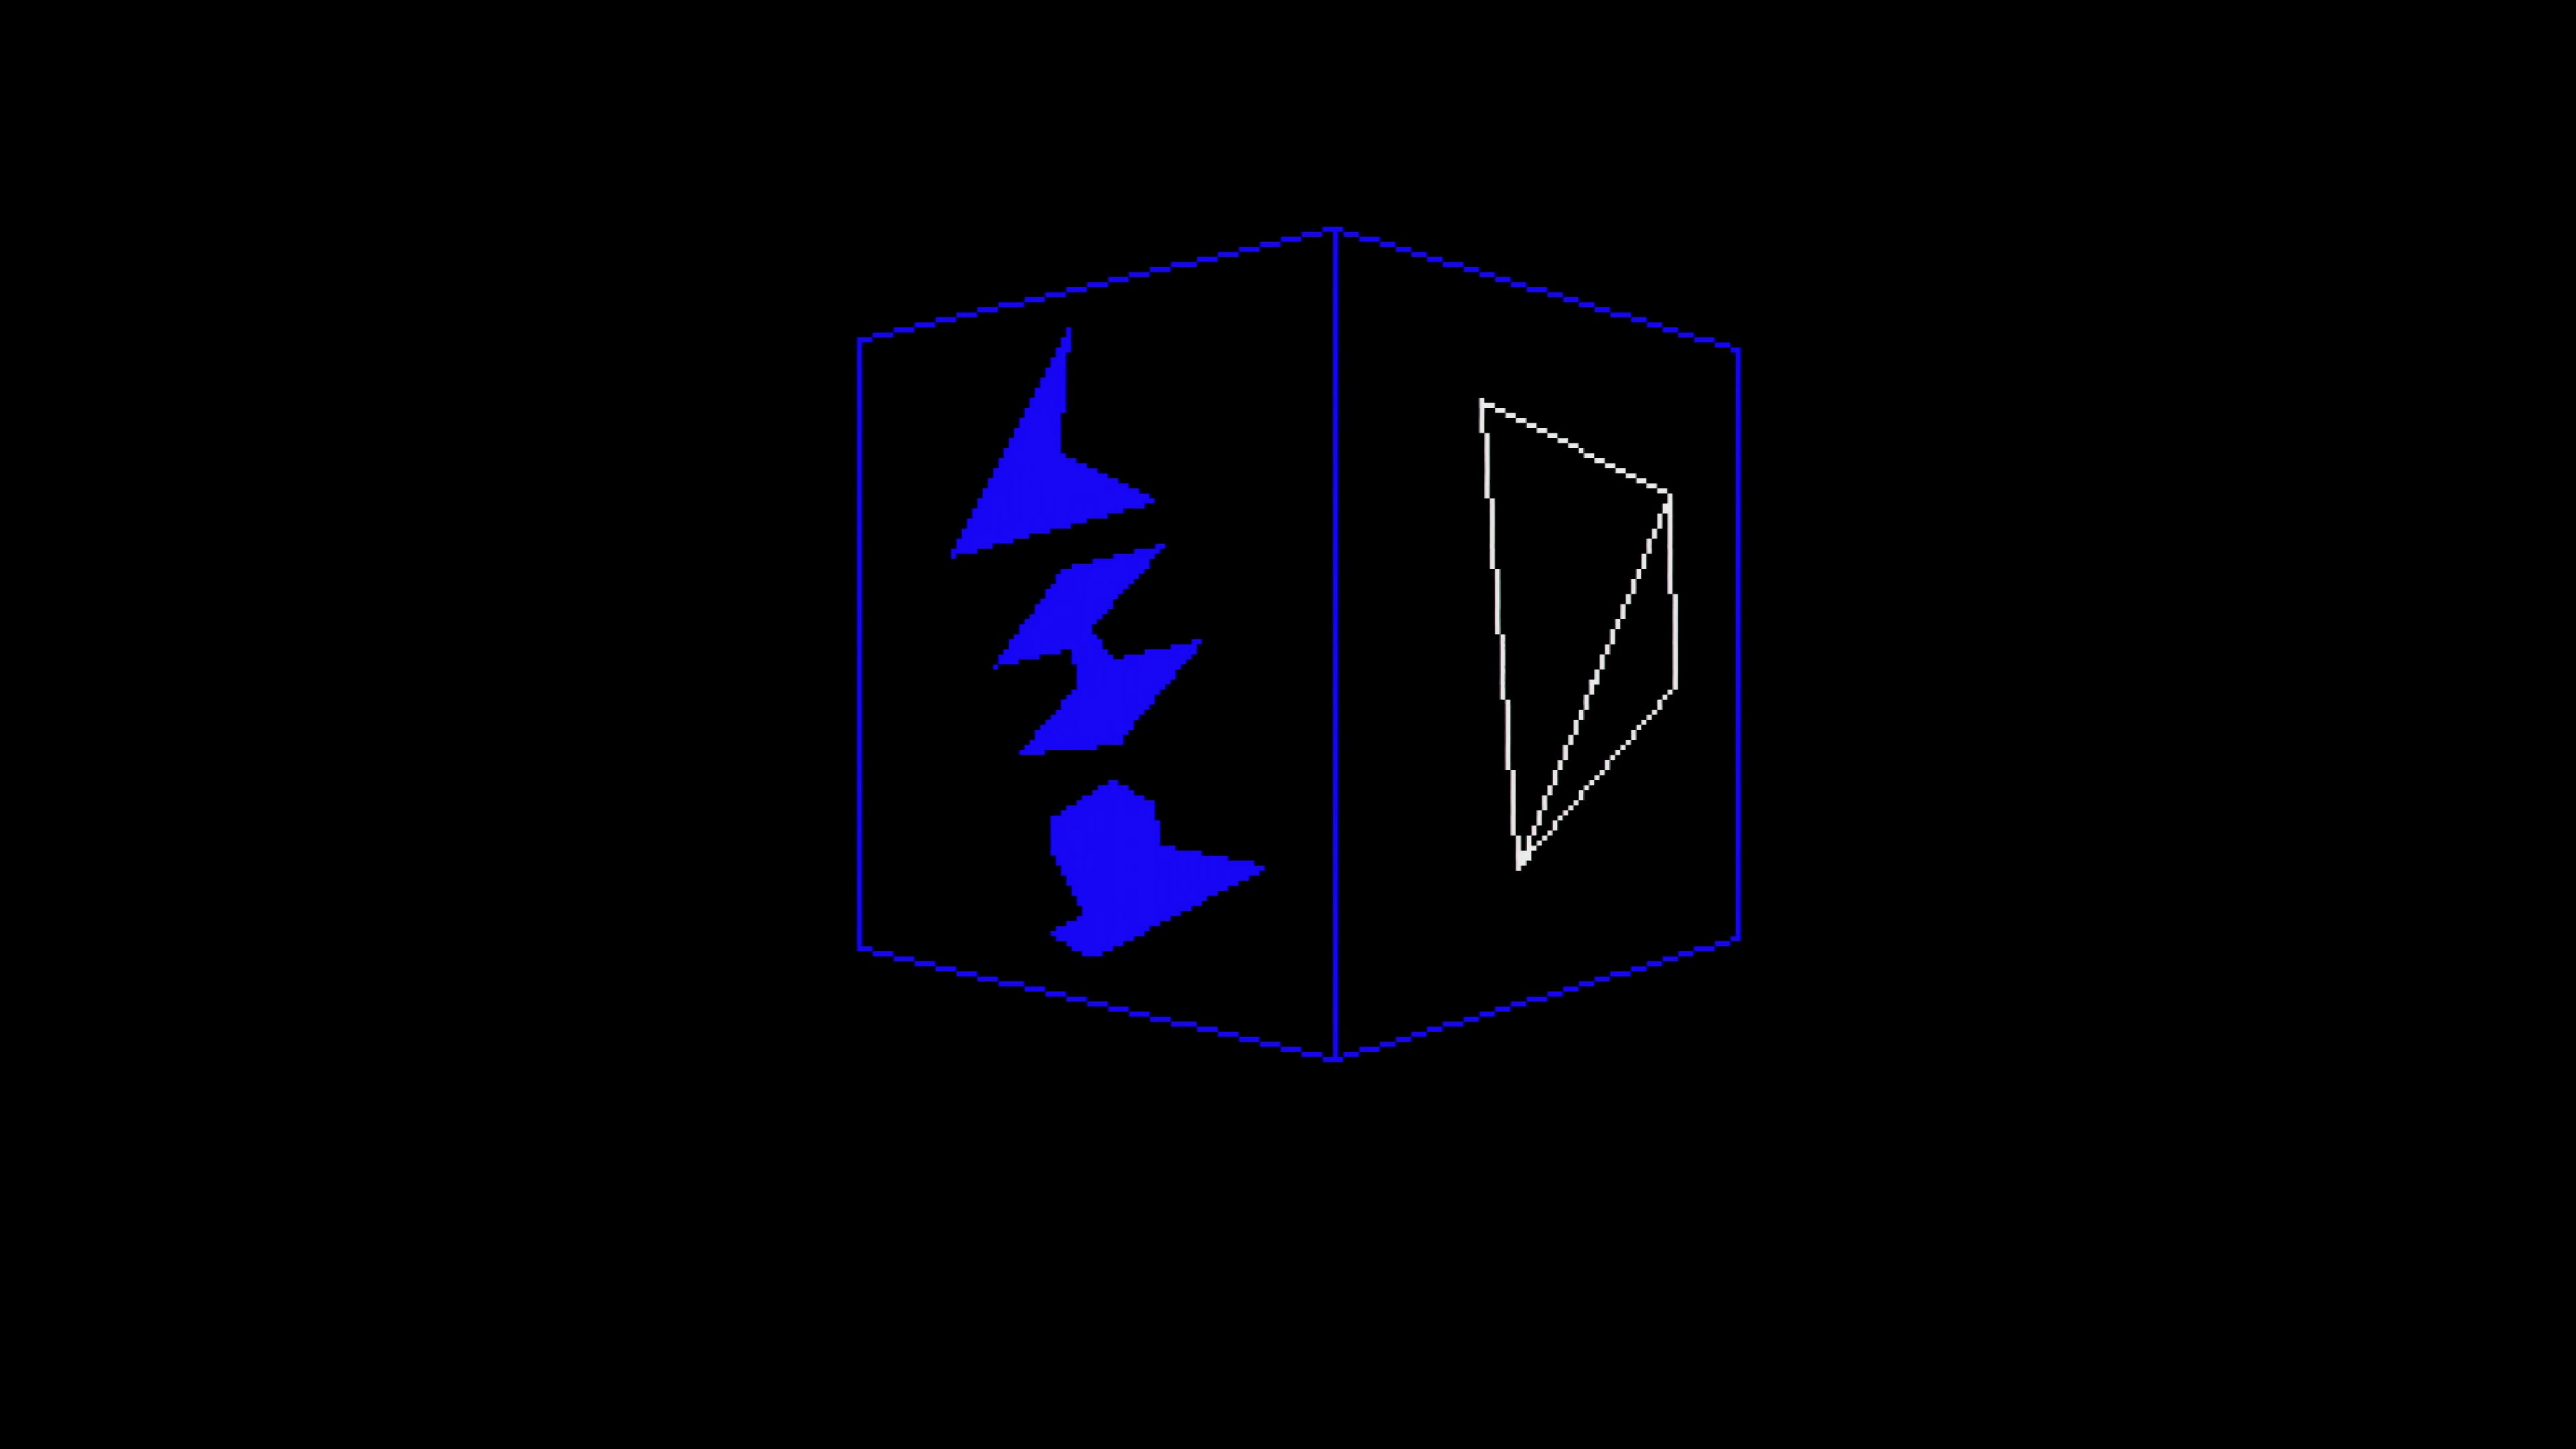
\includegraphics[width=\linewidth]{images/demoscene/demos/pheno1.png}
  \end{minipage}
  \hfill
  \begin{minipage}[b]{0.30\linewidth}
    \centering
    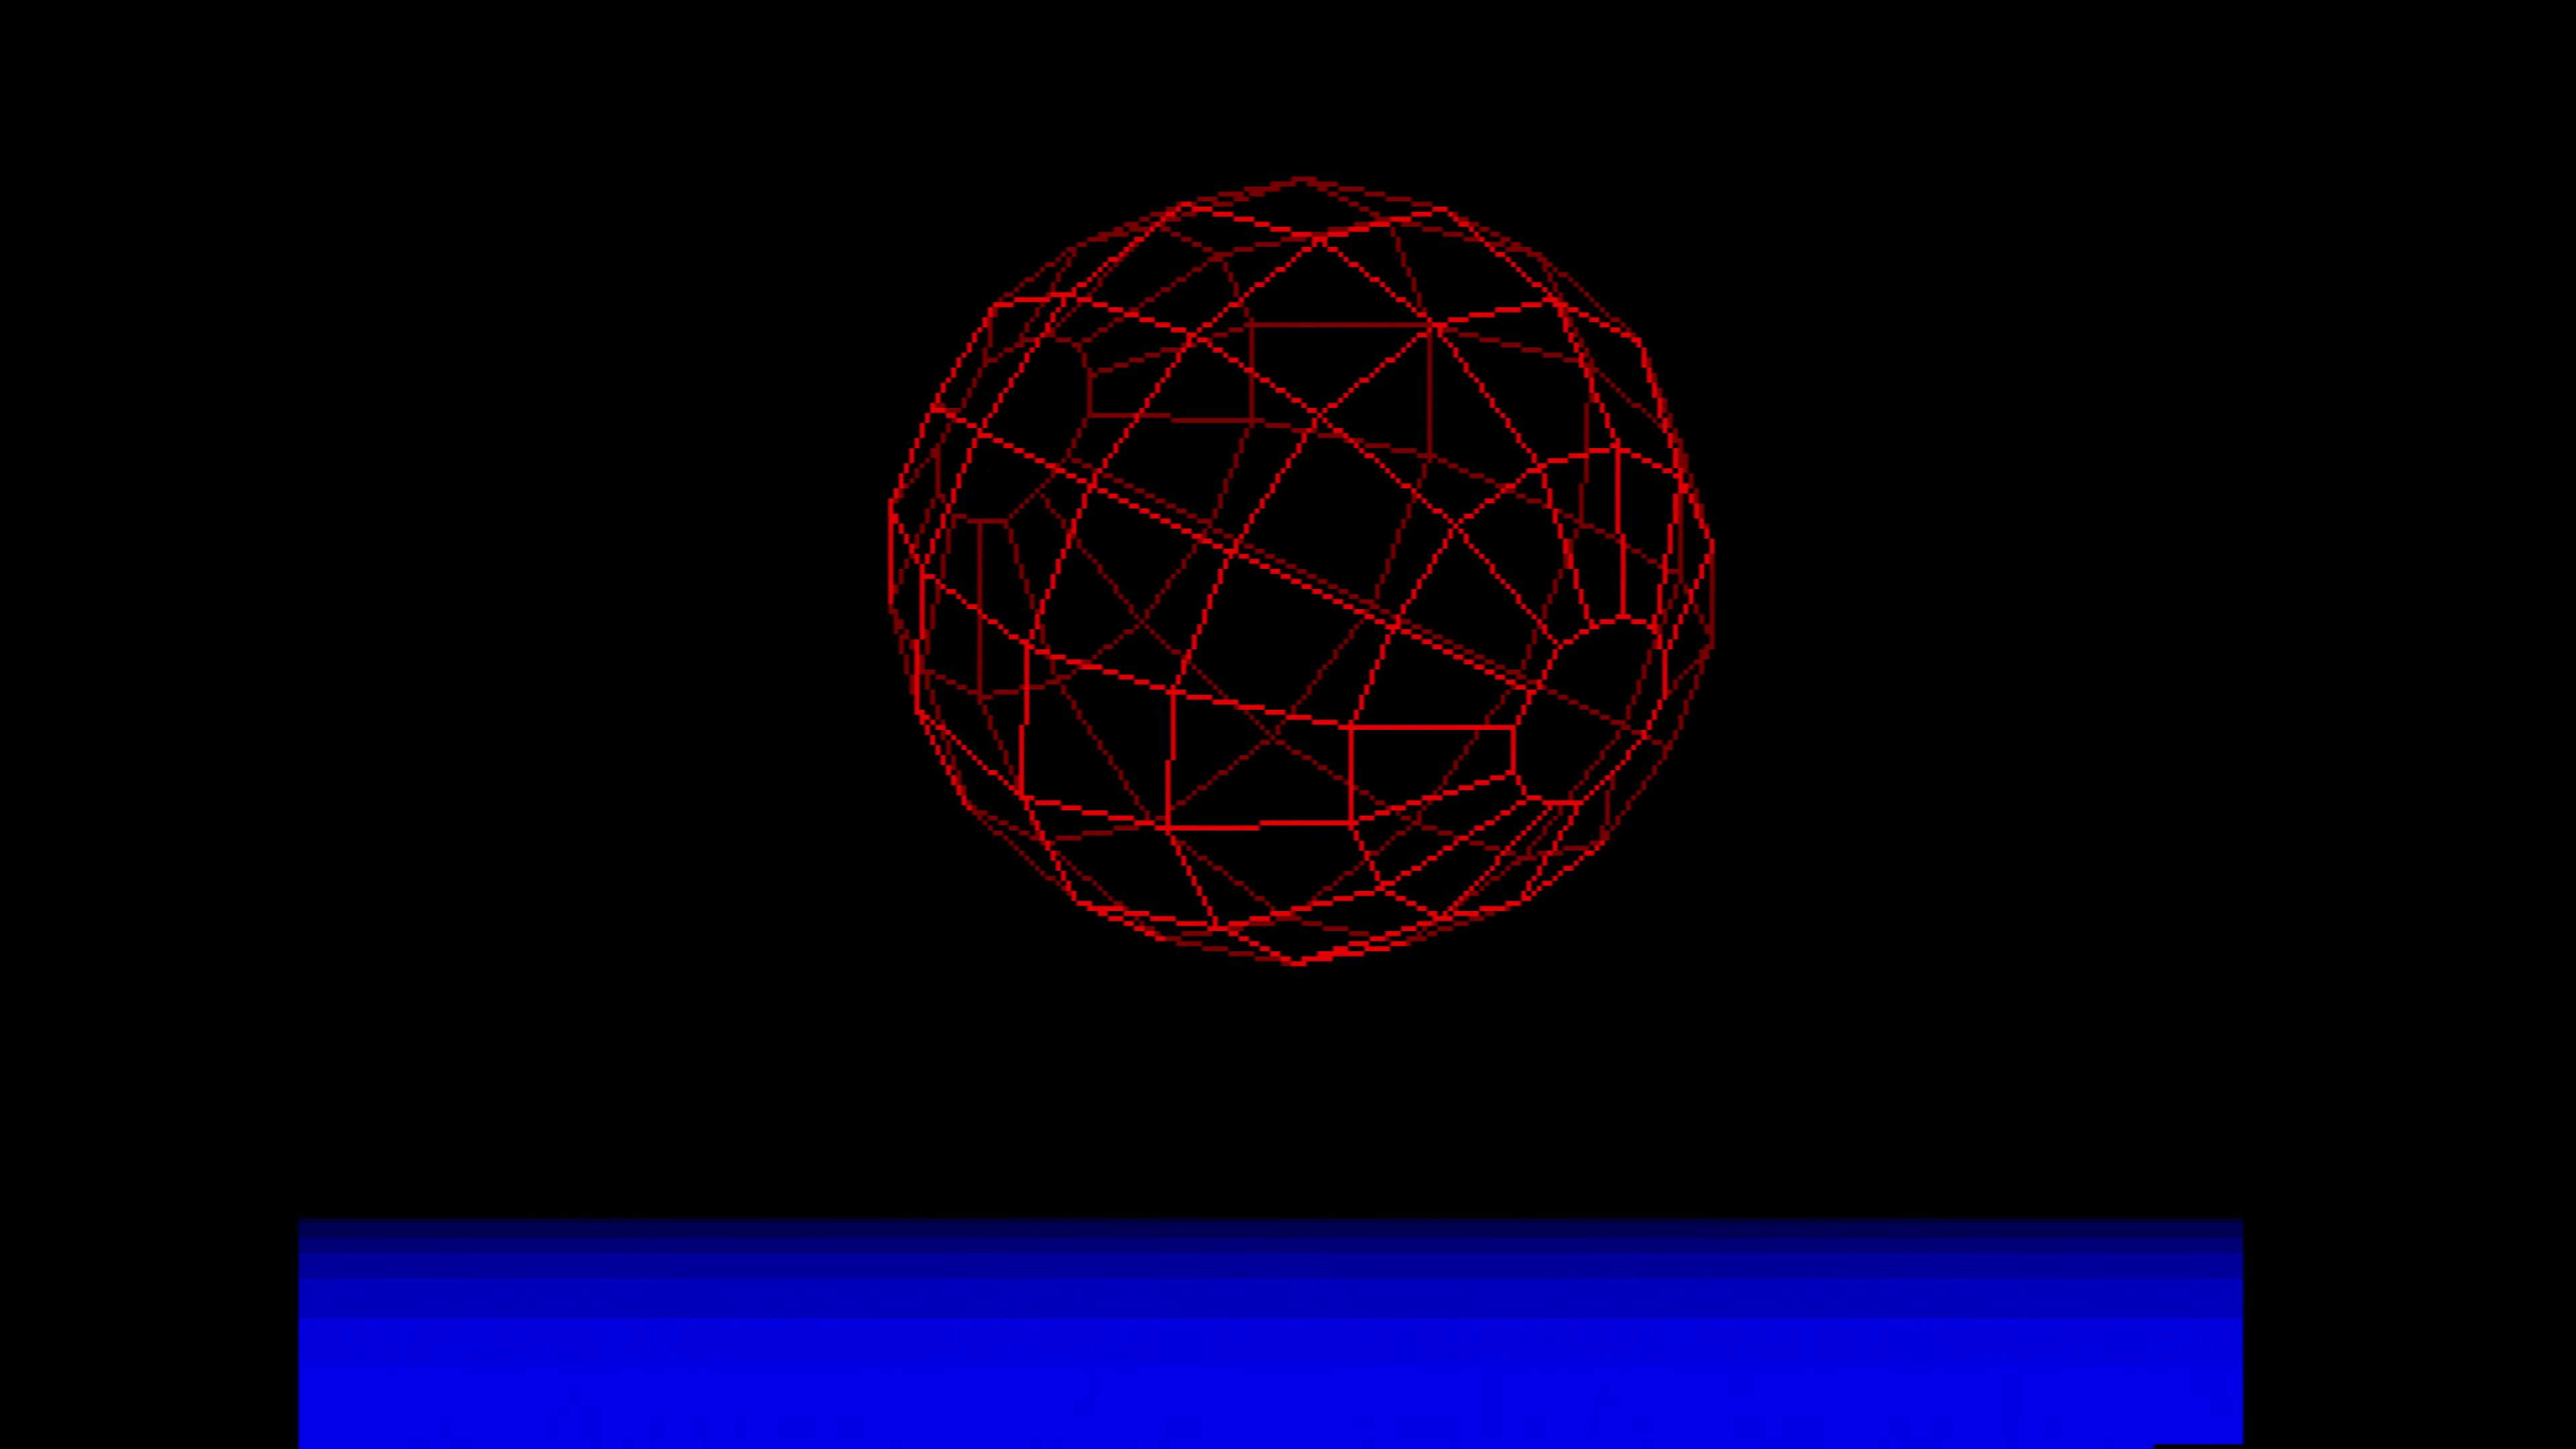
\includegraphics[width=\linewidth]{images/demoscene/demos/pheno2.png}
  \end{minipage}
  \hfill
  \begin{minipage}[b]{0.30\linewidth}
    \centering
    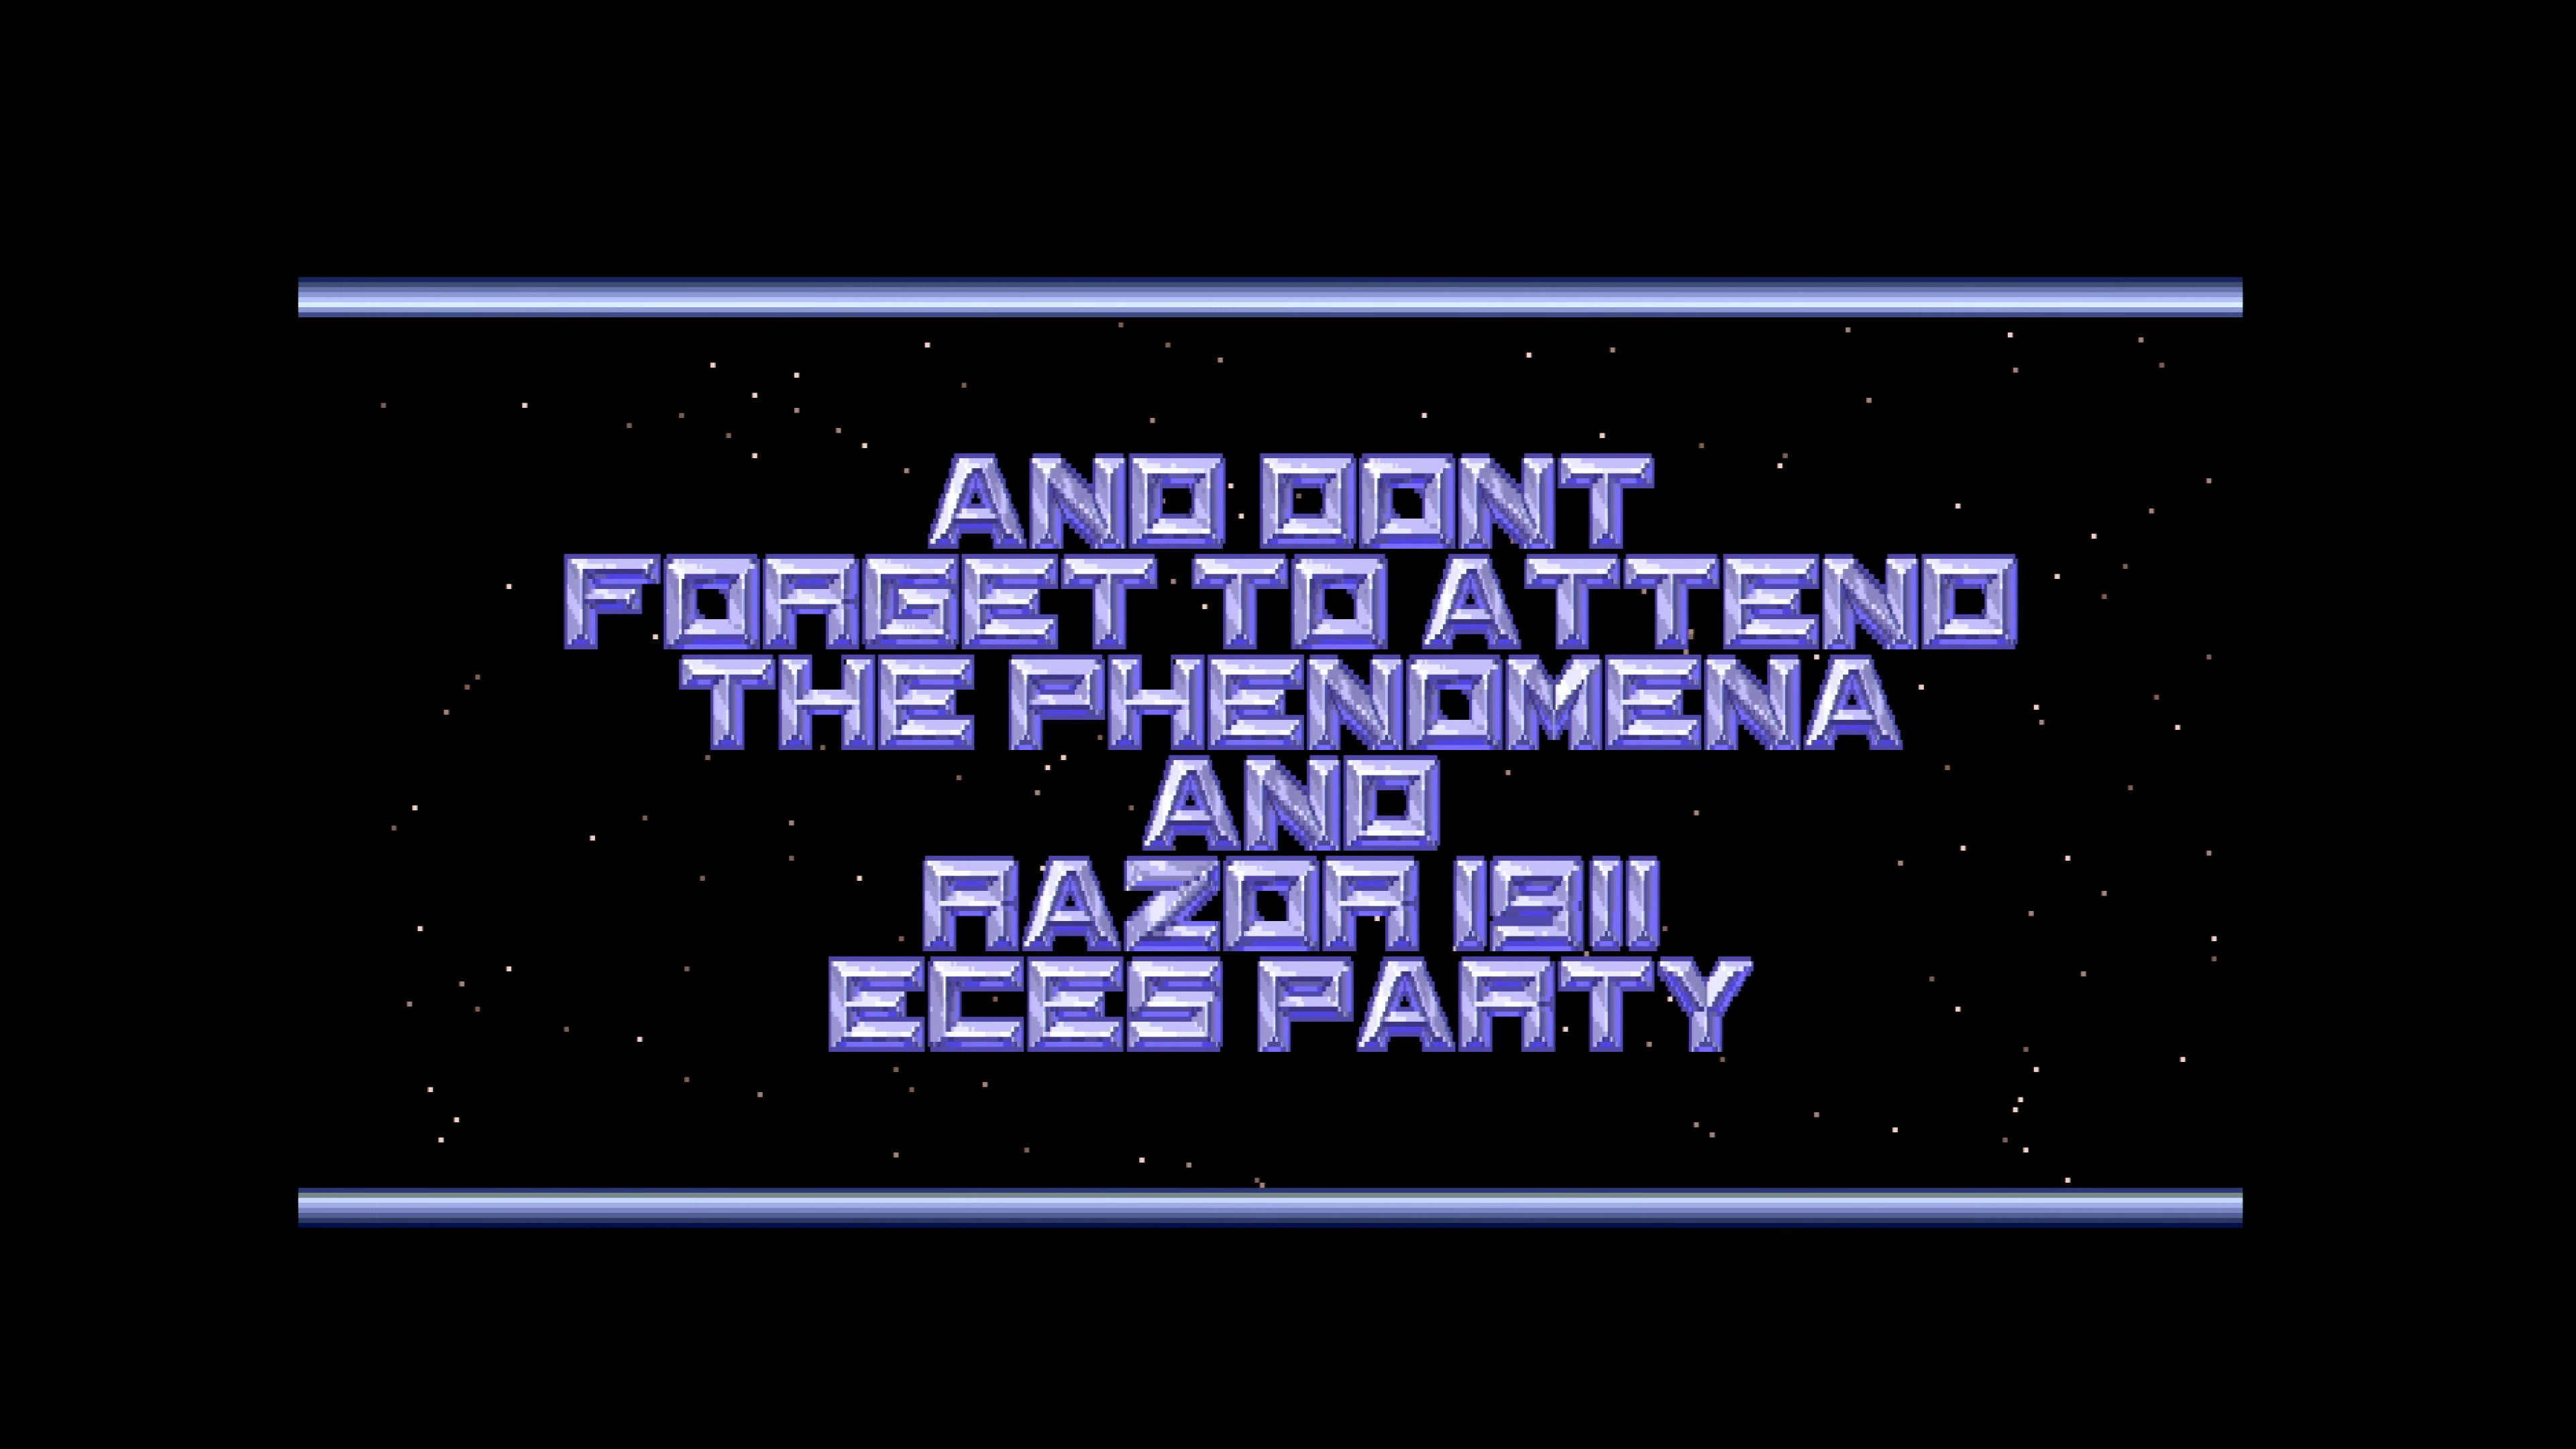
\includegraphics[width=\linewidth]{images/demoscene/demos/pheno3.png}
  \end{minipage}
  \caption{Phenomena- Enigma}
  \label{pheno}
\end{figure}

L'année 1984 marque un tournant dans l'histoire des \textit{crackers} et de la scène du piratage informatique. À cette époque, de nombreux groupes ont émergé, chacun avec sa propre spécialité et sa réputation dans le milieu. Parmi les plus influents, on retrouve des groupes comme TBC, connu pour avoir cracké des jeux populaires tels que «~Kennedy Approach~» ou «~Crackman Crew~».

Les membres de ces groupes n'étaient pas seulement experts en \textit{cracking}, ils étaient aussi capables d'adapter les jeux NTSC\footnote{NTSC (\textit{National Television System Committee}) est un système de codage couleur utilisé dans les émissions de télévision et de vidéo analogiques en Amérique du Nord, au Japon et dans certaines autres régions.} destinés au marché américain pour les rendre compatibles avec les systèmes PAL\footnote{PAL (\textit{Phase Alternating Line}) est un système de codage couleur utilisé dans les émissions de télévision et de vidéo analogiques dans de nombreuses régions, notamment en Europe, en Australie, en Chine et en Afrique.} utilisés en Europe. Cette adaptation était essentielle pour permettre aux joueurs européens de profiter des jeux américains sur leurs machines locales.

Outre TBC, d'autres groupes européens ont marqué le paysage du \textit{cracking}. Au Royaume-Uni, Yak Society s'est distingué en crackant les jeux de l'éditeur Elite, tandis qu'en Allemagne, des groupes comme Section 8 et ABC ont également laissé leur empreinte.


\subsection*{Le rôle central des \textit{swappers} dans la distribution}



La distribution de ces jeux piratés se réalisait de manière analogique, principalement par le biais de la voie postale. Les acteurs clés de cette dynamique étaient les \textit{swappers}\footnote{Les \textit{swappers} échangent généralement des \textit{demos}, des \textit{intros}, des musiques, des graphiques et d'autres types de productions créatives via des supports physiques comme des disquettes ou des cassettes, ou encore via des services en ligne lorsque l'Internet est devenu plus accessible.}, des individus passionnés qui avaient établi des réseaux de contacts à l'échelle mondiale. Ces échanges étaient le moteur de la circulation des \textit{cracktros}, des jeux et des logiciels au sein de la communauté. À travers l'envoi de disquettes par courrier postal, ces \textit{swappers} facilitaient la diffusion des créations artistiques, contribuant ainsi à la vitalité et à la croissance de la \textit{demoscene}. Ces échanges ne se limitaient pas seulement à la distribution de contenus, mais renforçaient également les liens entre les membres de la communauté, créant un réseau solide et engagé autour de la passion commune pour la création numérique.

\subsection*{Législation et évolution technique}

\begin{figure}[h]
  \begin{minipage}[b]{0.30\linewidth}
    \centering
    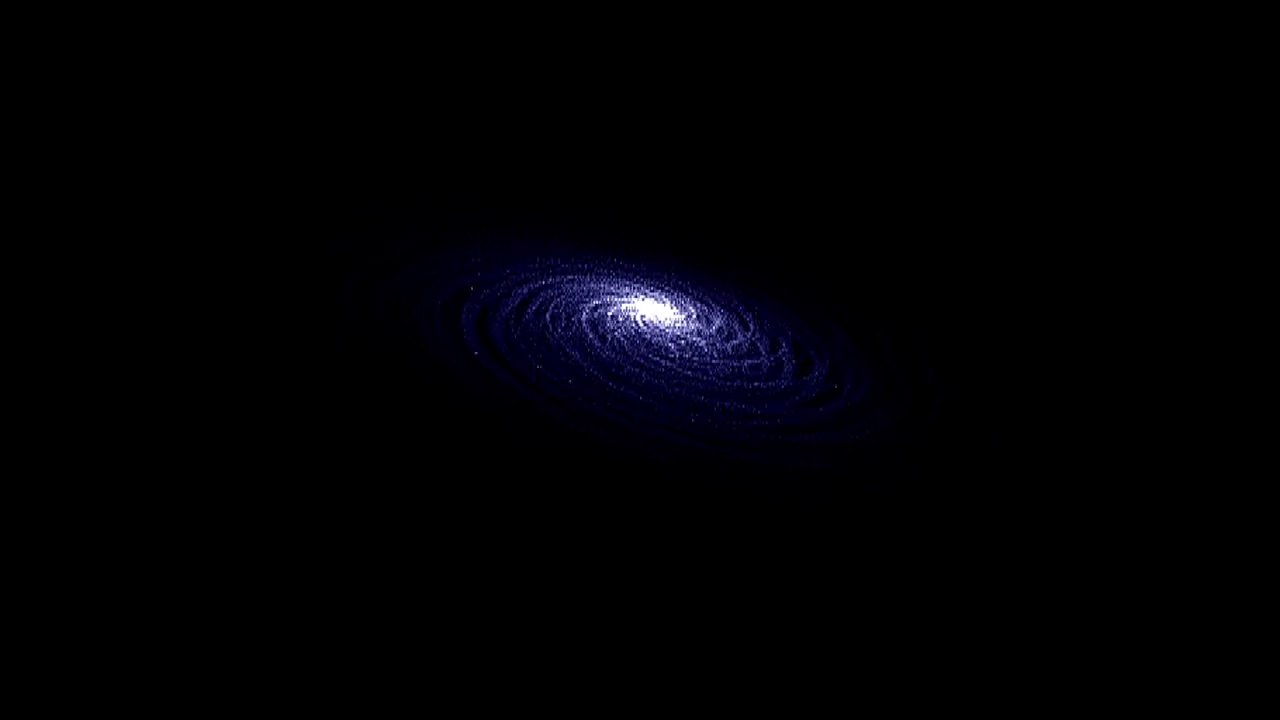
\includegraphics[width=\linewidth]{images/demoscene/demos/andromeda1.png}
  \end{minipage}
  \hfill
  \begin{minipage}[b]{0.30\linewidth}
    \centering
    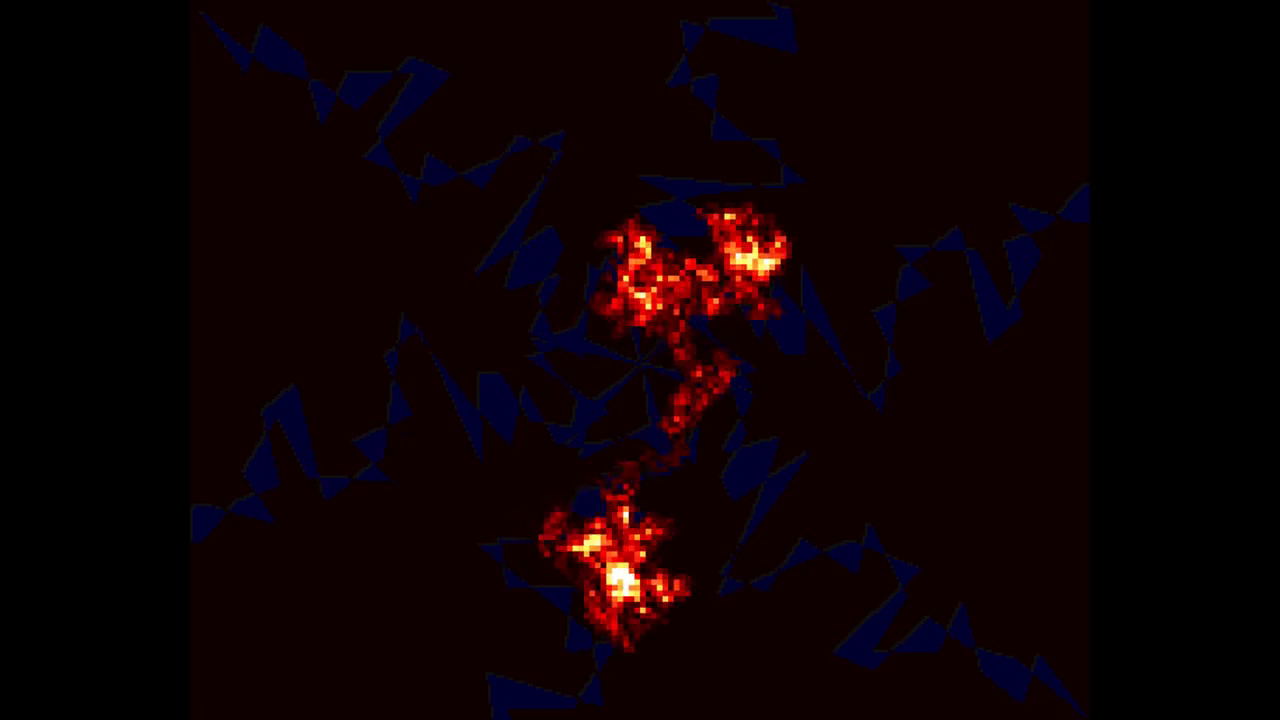
\includegraphics[width=\linewidth]{images/demoscene/demos/andromeda2.png}
  \end{minipage}
  \hfill
  \begin{minipage}[b]{0.30\linewidth}
    \centering
    
\includegraphics[width=\linewidth]{images/demoscene/demos/andromeda3.png}
  \end{minipage}
  \caption{Nexus 7 - Andromeda}
  \label{andromeda}
\end{figure}


Les éditeurs de jeux ont rapidement réagi pour essayer de contrôler la diffusion de ces copies piratées alors qu'elles se propageaient. Au milieu des années 80, face à l'ampleur du phénomène, une législation a été mise en place en Europe et aux États-Unis visant à interdire toute modification, duplication ou distribution non autorisée de logiciels commerciaux.

Cette réglementation visait à protéger les droits d'auteur des éditeurs et à décourager le piratage des jeux. Elle a marqué un tournant dans l'histoire de la communauté du Commodore 64, mettant fin à l'ère de la duplication libre et créant un contexte juridique plus contraignant pour les amateurs de jeux piratés et les \textit{crackers}.

Cette évolution légale a poussé certains membres de la communauté à s'orienter vers des pratiques plus créatives et légales, donnant naissance à la \textit{demoscene} et à la création d'\textit{intros}\footnote{Une \textit{intro} (abréviation de « introduction ») est une petite production \textit{demo}, souvent de courte durée, conçue pour montrer les compétences et la créativité d'un groupe ou d'un individu. Contrairement aux \textit{demos} complètes qui peuvent durer plusieurs minutes, les \textit{intros} sont généralement plus courtes, parfois limitées à quelques dizaines de secondes, et se concentrent sur un effet ou une idée particulière.} originales, loin des pratiques de piratage. Malgré cela la créativité des \textit{crackers} n'a pas été freinée. De nouvelles techniques ont rapidement émergé pour contourner les mesures de protection des jeux.

La première méthode de \textit{crack} qui a vu le jour était le \textit{reset cracking}. Cette méthode était relativement simple : en appuyant sur le bouton de réinitialisation (le \textit{reset}) du Commodore 64, le contenu de la mémoire restait intact, permettant ainsi aux \textit{crackers} d'accéder au programme en cours d'exécution. En gelant le programme, ils étaient alors en mesure d'extraire et de modifier les données. Par la suite, des modules de gel sur support cartouche ont été développés. Ces cartouches offraient la possibilité de geler le système sans avoir besoin de réinitialiser l'ordinateur, rendant la manipulation encore plus aisée et rapide pour les \textit{crackers}.

Cette course à l'armement entre \textit{crackers} et éditeurs a contribué à enrichir les compétences techniques de la communauté, ouvrant la voie à de nouvelles formes d'expression et à l'émergence de la \textit{demoscene}.


% \todo{déplacer vers la section sur l \textit{elite} de la \textit{scene}}

\subsection*{Cracking et élitisme: les codes de la culture \textit{demoscene}}
La culture du \textit{cracking} a également développé ses propres codes et valeurs. L'élitisme et l'avant-gardisme en opposition aux \textit{lamers}\footnote{Le terme \textit{lamer} est généralement utilisé de manière péjorative pour décrire quelqu'un qui prétend avoir des compétences ou des connaissances qu'il ne possède pas réellement.} sont devenus des caractéristiques marquantes de la scène, reflétant la volonté des membres de se démarquer et de repousser les limites de ce qui est possible. De nombreux adolescents ont été inspirés par cette culture et ont rêvé de devenir un jour un \textit{cracker} de renom, contribuant ainsi à la croissance et à la pérennité de la \textit{demoscene}.


\subsection*{La réponse de l'élite de la scène aux surveillances du FBI}
\begin{figure}[h]
  \begin{minipage}[b]{0.30\linewidth}
    \centering
    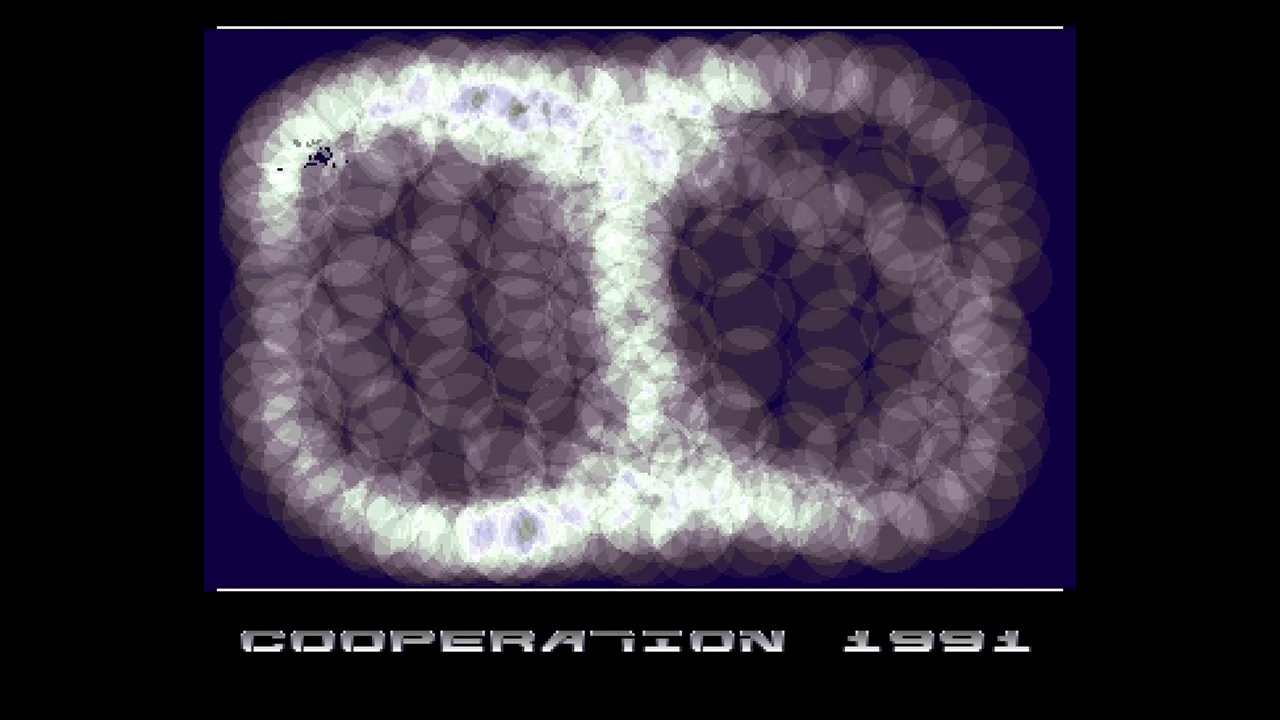
\includegraphics[width=\linewidth]{images/demoscene/demos/crio1.png}
  \end{minipage}
  \hfill
  \begin{minipage}[b]{0.30\linewidth}
    \centering
    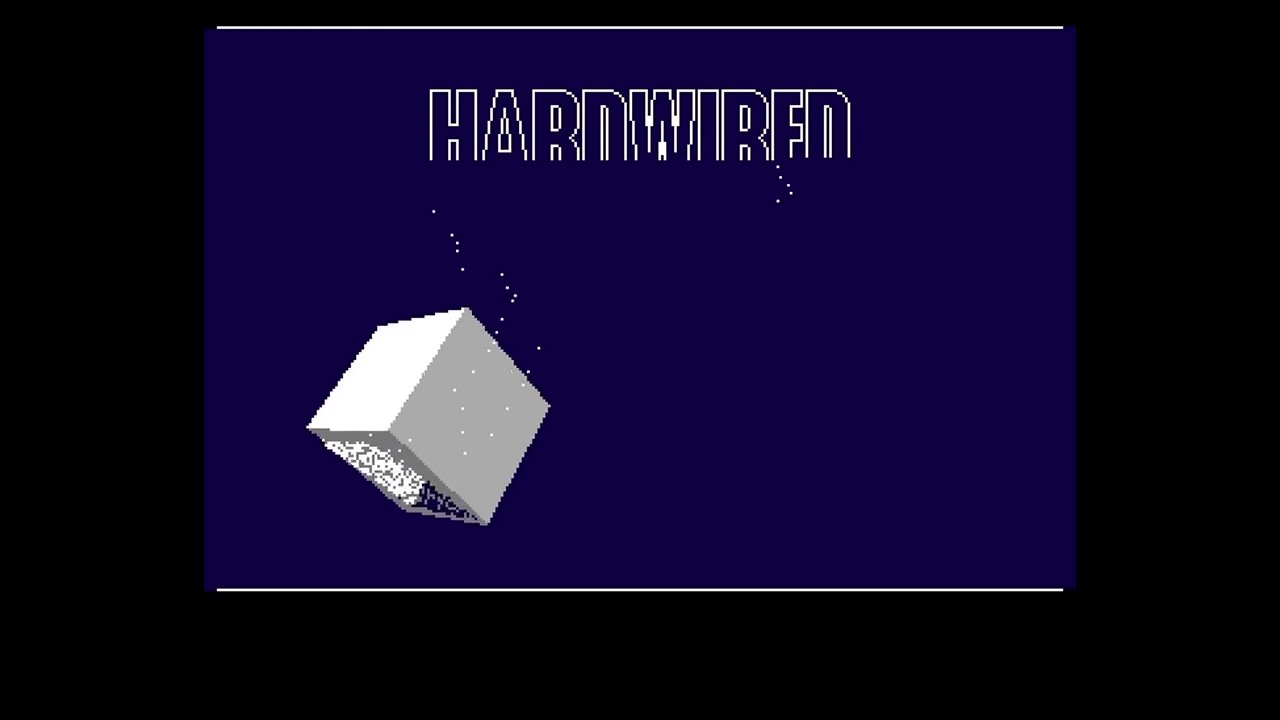
\includegraphics[width=\linewidth]{images/demoscene/demos/crio2.png}
  \end{minipage}
  \hfill
  \begin{minipage}[b]{0.30\linewidth}
    \centering
    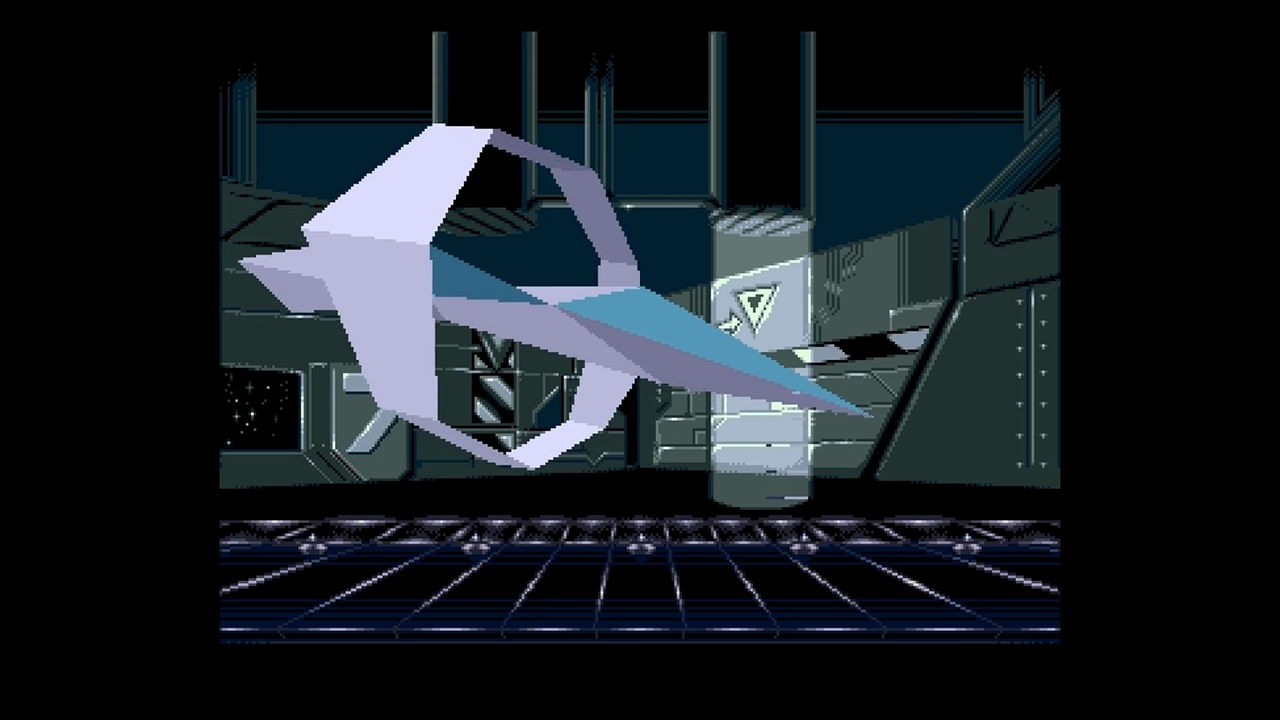
\includegraphics[width=\linewidth]{images/demoscene/demos/crio3.png}
  \end{minipage}
  \caption{The Silents \& Crionics - Hardwired}
  \label{crio}
\end{figure}


Face à la surveillance accrue du FBI (\textit{Federal Bureau of Investigation}), les \textit{crackers} ont rapidement ajusté leurs méthodes pour échapper à la détection. L'élite\footnote{L'élite fait référence aux individus ou groupes qui se distinguent par leurs compétences techniques, leur innovation, et leur contribution significative à la culture et à l'art de la \textit{demoscene}.} de la scène a développé des techniques pour brouiller les pistes et rendre leur communication moins suspecte.

Le FBI mettait en place des systèmes de surveillance des lignes téléphoniques en utilisant des ordinateurs pour détecter certains mots-clés ou phrases suspects. Afin d'éviter cette surveillance, les \textit{crackers} ont commencé à utiliser ce qu'on appelle maintenant le \textit{leet speak}\footnote{Le \textit{leet speak} (ou \textit{l33t speak}) est un langage codé utilisant des substitutions de lettres, des chiffres et des symboles spéciaux pour remplacer les lettres originales, rendant la communication plus cryptique et réservée à ceux qui connaissent ce langage.}. Ils ont altéré les mots et les phrases de façon à les rendre méconnaissables pour les systèmes de surveillance.

À titre d'exemple, le terme \textit{wares}, faisant référence aux logiciels piratés, a été modifié en \textit{warez}, tandis que la lettre «~O~» a été substituée par le chiffre zéro («~0~»). D'autres substitutions étaient également courantes, comme remplacer la lettre « A » par le chiffre quatre («~4~»). Certains ont même utilisé des caractères spéciaux ou des lettres de l'alphabet non latin pour brouiller davantage les pistes.

Cette pratique du \textit{leet speak} n'était pas seulement une manière de contourner la surveillance, mais aussi un moyen pour la communauté de se démarquer et de créer un langage propre à leur culture. Cette forme d'argot électronique a perduré au fil du temps et est encore utilisée aujourd'hui, notamment dans les pseudonymes et les communications sur Internet. Elle témoigne de l'ingéniosité et de la résilience de la \textit{demoscene} face aux défis et aux menaces externes.

\subsection*{D'un monde de \textit{cracking} à l'industrie légale}

Malgré leurs débuts dans le piratage et le \textit{cracking}, ces experts en informatique ont su mettre leurs compétences au service de l'industrie de manière légale et productive. Leur expérience dans le \textit{cracking} leur a souvent donné un avantage unique, leur permettant de comprendre en profondeur les systèmes et les logiciels, et de contribuer de manière significative au développement technologique et informatique. Cette transition illustre bien la complexité et la dualité de la scène du \textit{cracking}, où les frontières entre le légal et l'illégal, entre le jeu et le travail, sont parfois floues. Leurs compétences sont particulièrement prisées dans des secteurs comme le développement de jeux vidéo, l'animation, les effets spéciaux et la post-production.

Bon nombre de professionnels éminents de l'industrie du jeu vidéo et de l'animation ont fait leurs premiers pas dans la scène \textit{demo}. Cette dernière offre en effet une plateforme unique pour l'expérimentation, le \textit{feedback} en temps réel de la communauté et le perfectionnement des compétences. Elle constitue ainsi un tremplin exceptionnel pour une carrière réussie dans les domaines créatifs et technologiques.

Les groupes DICE\footnote{DICE, ou Digital Illusions Creative Entertainment, est un studio de développement de jeux vidéo basé en Suède. Fondé en 1992 par Olof Gustafsson et Markus Nyström, le studio est surtout connu pour ses franchises à succès comme « Battlefield », « Mirror's Edge » et « Star Wars Battlefront ».} et Remedy\footnote{Remedy Entertainment est un studio finlandais de jeux vidéo connu pour ses jeux narratifs innovants tels que « Max Payne », « Alan Wake », « Quantum Break » et « Control ». Situé à Espoo, il est reconnu pour ses histoires captivantes et sa maîtrise de la narration interactive.} illustrent parfaitement comment des groupes de \textit{demosceners} ont su transformer leur passion et leur talent en des carrières accomplies au sein de l'industrie du jeu vidéo. Ces \textit{success stories} soulignent l'impact considérable que la créativité et l'innovation de la scène \textit{demo} peuvent avoir, transcendant ainsi les limites traditionnelles de cette communauté. En outre, il est important de souligner que de nombreux musiciens issus de la scène \textit{demo} ont saisi des opportunités professionnelles dans la composition de bandes sonores pour des titres emblématiques tels qu'Assassin's Creed ou la série Unreal.



% Évolution de la demoscene
\newpage
\section{Évolution de la \textit{demoscene} vers les \textit{demoparties}}

%\subsection*{Introduction}
Nous allons maintenant aborder les divers facteurs qui ont contribué à l'évolution de la \textit{demoscene}, ainsi qu'examiner de plus près les techniques utilisées.

\begin{figure}[h]
  \begin{minipage}[b]{0.30\linewidth}
    \centering
    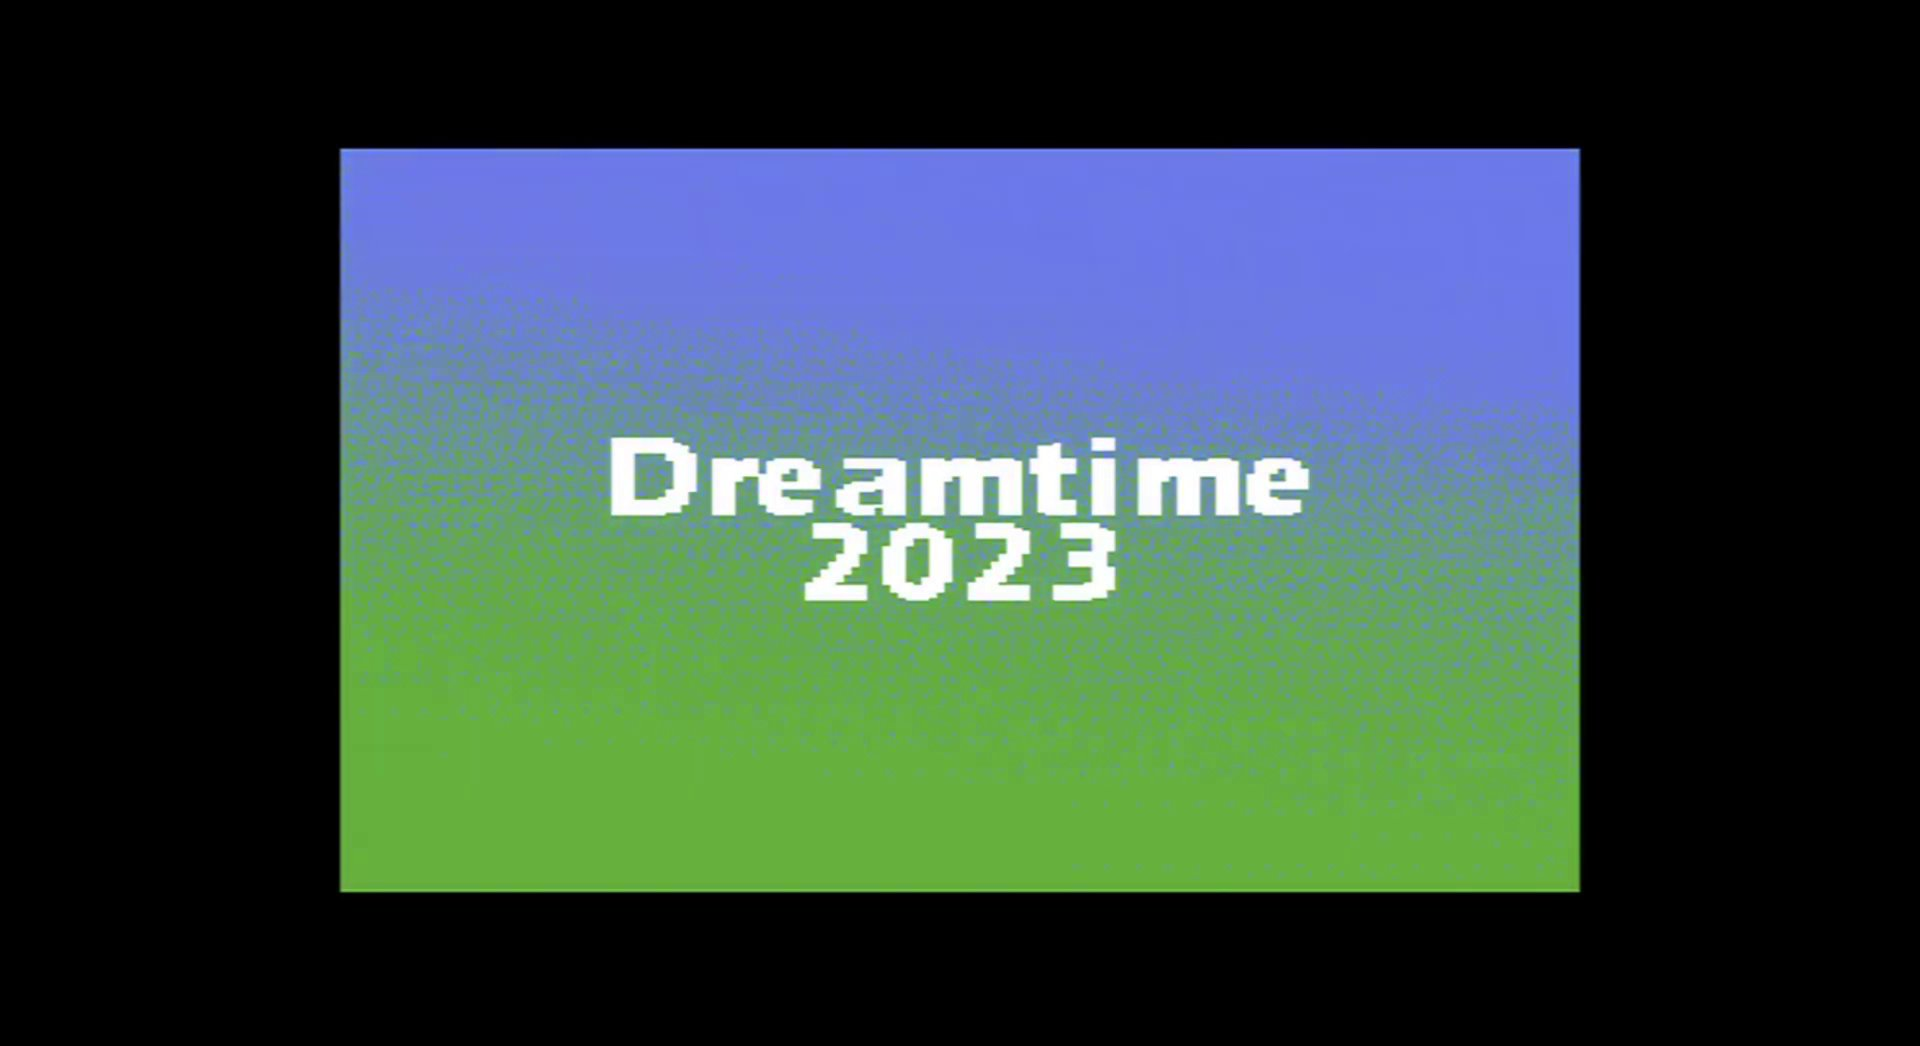
\includegraphics[width=\linewidth]{images/demoscene/demos/dreamtime1.png}
  \end{minipage}
  \hfill
  \begin{minipage}[b]{0.30\linewidth}
    \centering
    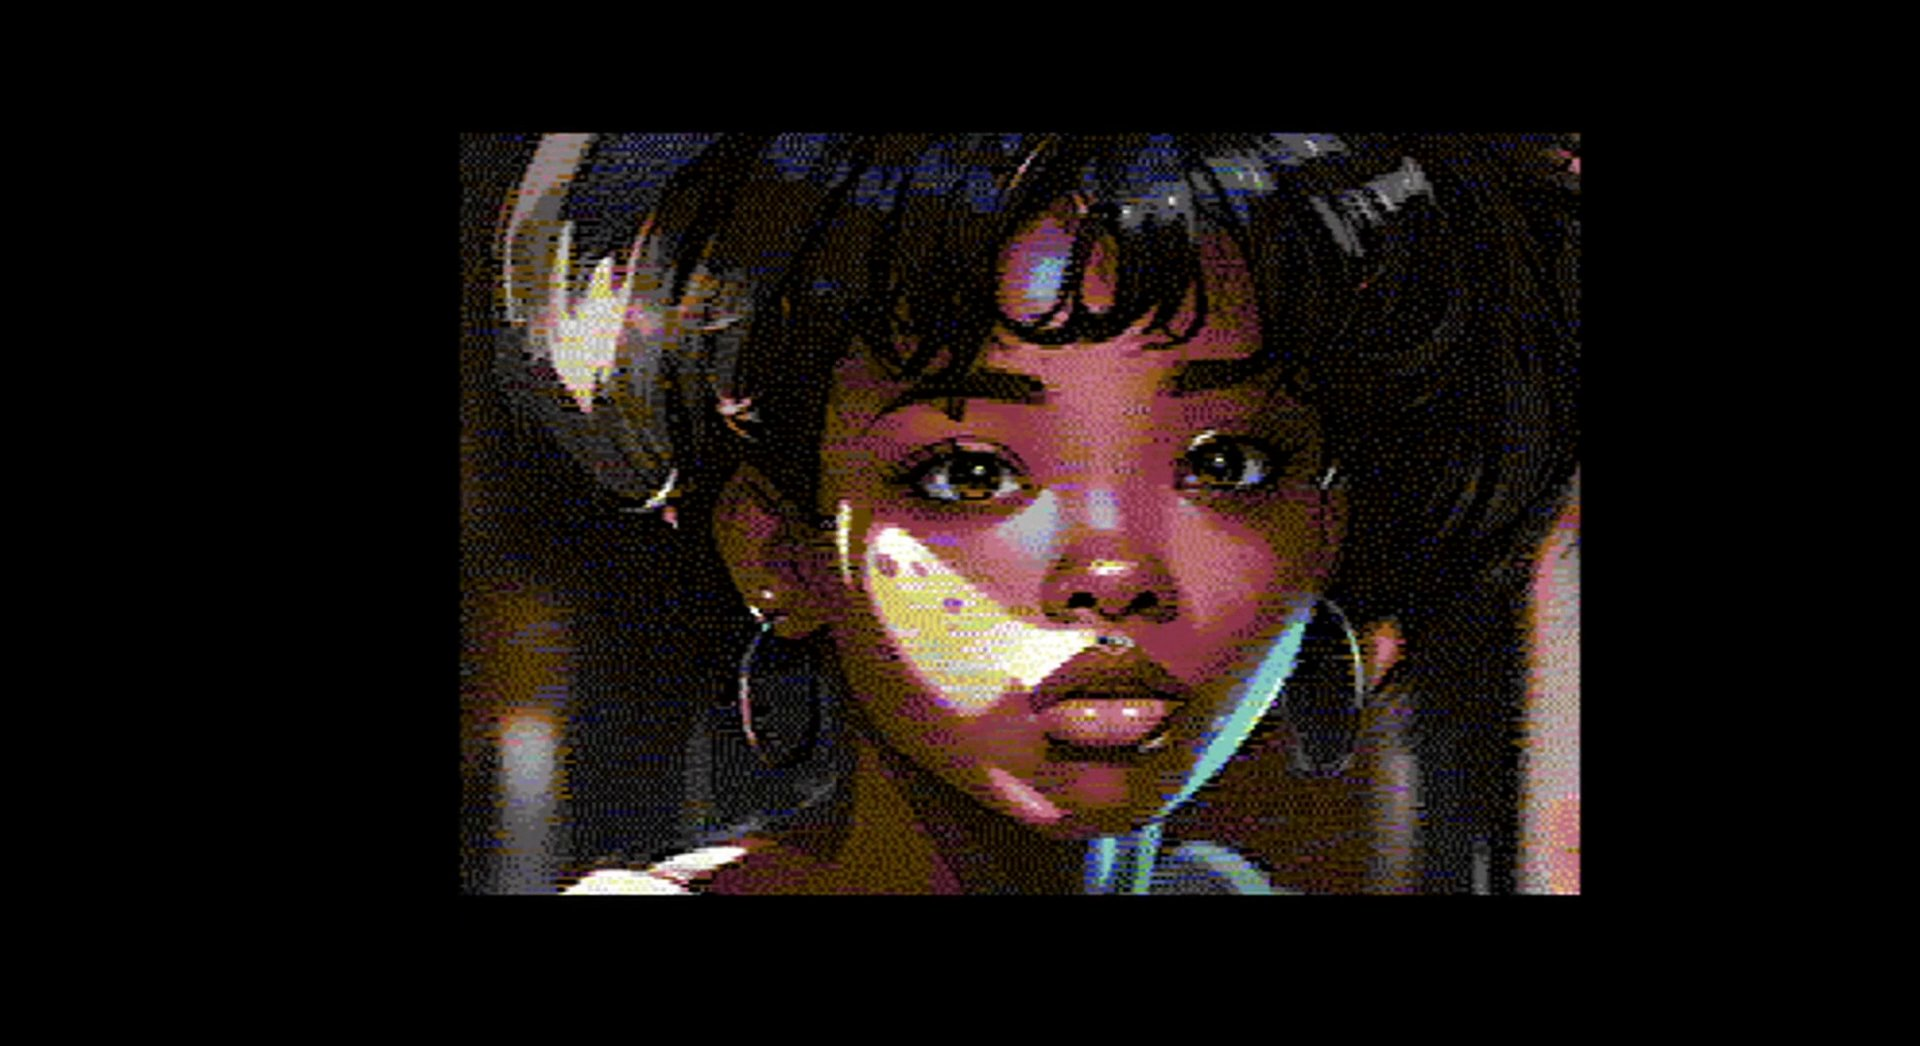
\includegraphics[width=\linewidth]{images/demoscene/demos/dreamtime2.png}
  \end{minipage}
  \hfill
  \begin{minipage}[b]{0.30\linewidth}
    \centering
    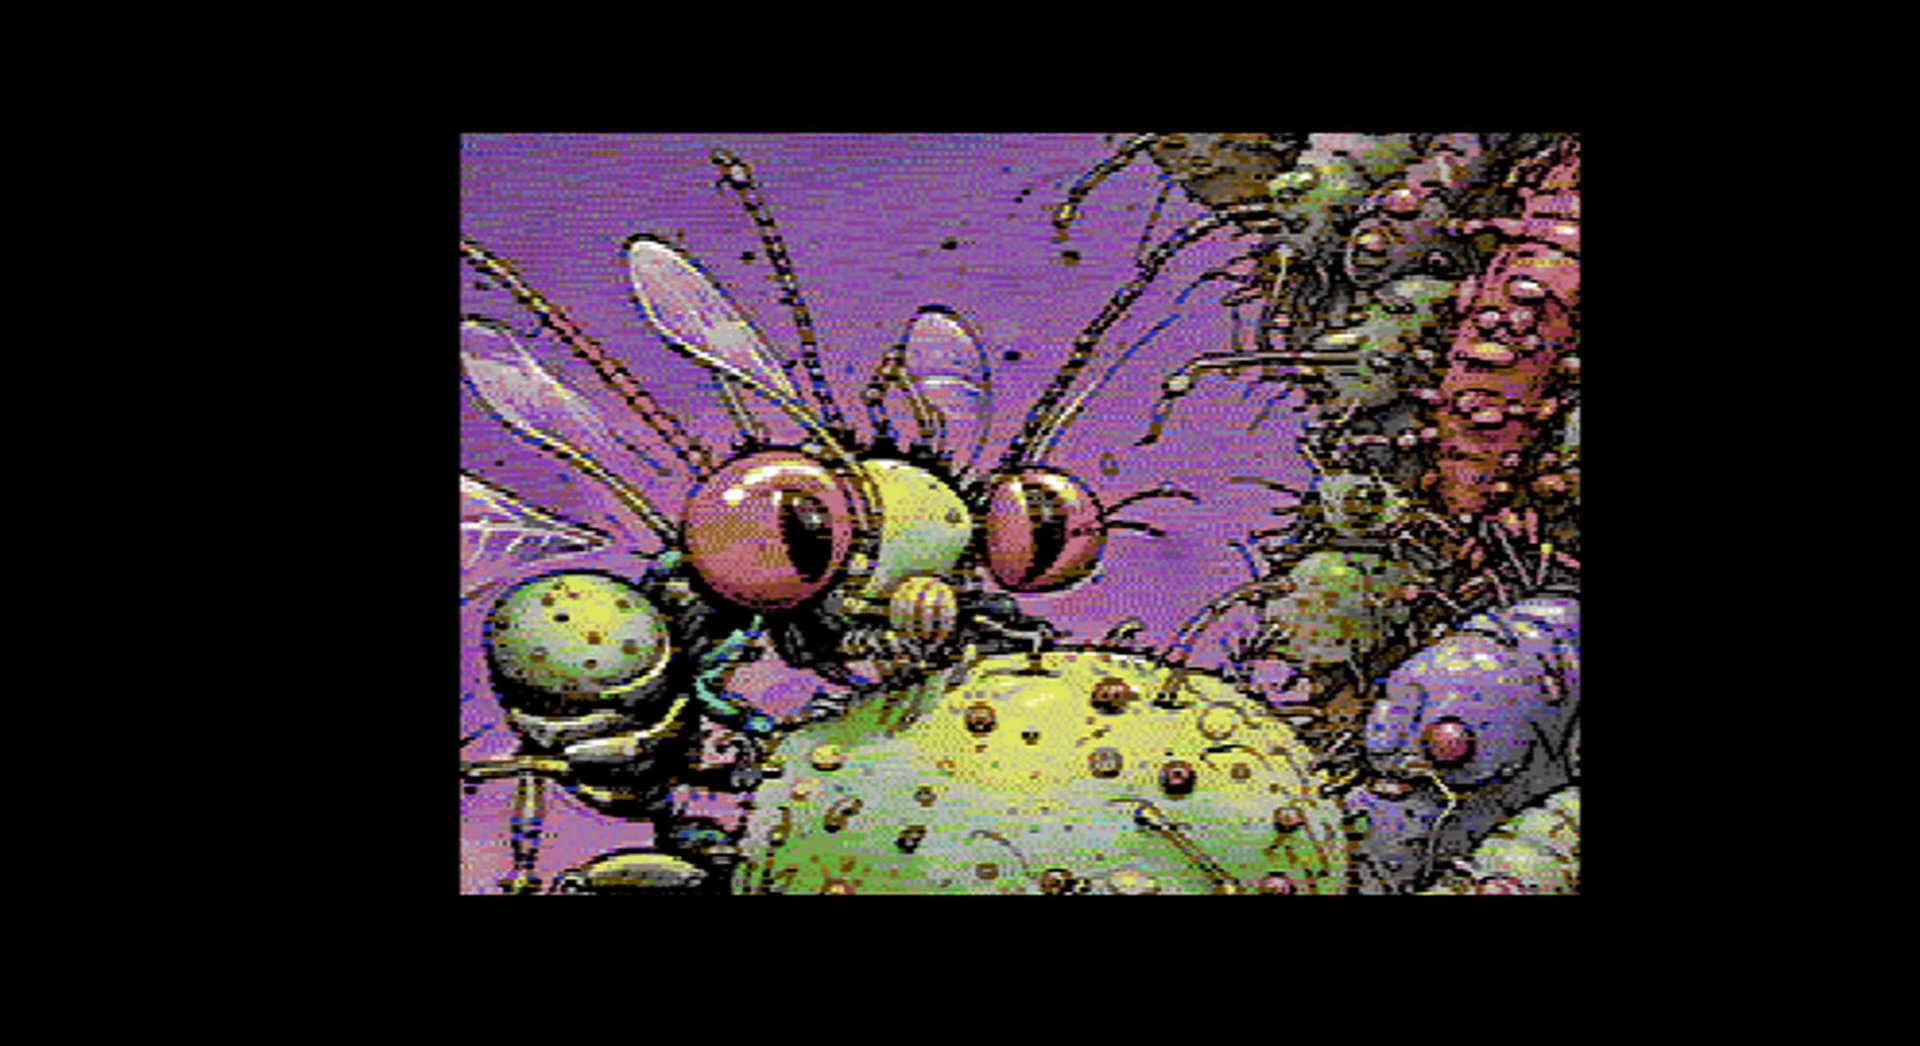
\includegraphics[width=\linewidth]{images/demoscene/demos/dreamtime3.png}
  \end{minipage}
  \caption{Dreamtime - Profik}
  \label{dreamtime}
\end{figure}



\subsection*{L'essor des \textit{demoparties} et la structuration de la communauté}

Si à l'origine l'objectif principal était de réussir le « crackage » d'un jeu, il est rapidement devenu évident que la création d'\textit{intros} de qualité était tout aussi cruciale pour se démarquer au sein de la communauté. C'est aussi vers le milieu des années 80 que la scène a véritablement pris de l'ampleur, se structurant de manière plus formelle. Les groupes de \textit{crackers} ont commencé à se rencontrer physiquement en organisant des rencontres et des rassemblements. Ces \textit{demoparties} étaient l'occasion pour les passionnés de l'informatique et de la \textit{demo} de se rencontrer, de partager leurs créations, et d'échanger des astuces ou des techniques de programmation. 

Les \textit{demos} se distinguent des \textit{cracktros} par leur complexité accrue et leur autonomie vis-à-vis des logiciels originaux. Elles ne se contentaient plus de présenter les capacités de \textit{cracking} des groupes, mais devenaient de véritables œuvres d'art combinant programmation, design et musique pour offrir une expérience immersive.

\subsection*{L'évolution artistique des signatures des \textit{crackers}}
L'évolution des signatures des \textit{crackers} reflète bien la transition de la scène du simple \textit{cracking} vers la création d'\textit{intros} plus élaborées. Initialement, la signature était une manière discrète pour le \textit{cracker} de laisser sa marque sur une copie piratée. Cette signature, souvent composée de trois lettres, rappelait les initiales utilisées dans les jeux d'arcade pour marquer les meilleurs scores. Elle servait à identifier l'auteur du \textit{crack}, tout en affirmant sa réputation au sein de la communauté. Cependant, avec l'émergence de la \textit{demoscene}, cette simple signature a rapidement évolué. Les \textit{crackers} ont commencé à utiliser les \textit{intros} comme un média pour afficher leur pseudonyme de manière plus graphique et artistique. Au lieu de se limiter à une combinaison de trois lettres, ils ont intégré leur pseudonyme dans des \textit{logos} aux animations complexes (voir \ref{logo}).

\begin{figure}[h]
  \begin{minipage}[b]{0.30\linewidth}
    \centering
    
\includegraphics[width=\linewidth]{images/demoscene/demos/logo1.png}
  \end{minipage}
  \hfill
  \begin{minipage}[b]{0.30\linewidth}
    \centering
    
\includegraphics[width=\linewidth]{images/demoscene/demos/logo2.png}
  \end{minipage}
  \hfill
  \begin{minipage}[b]{0.30\linewidth}
    \centering
    
\includegraphics[width=\linewidth]{images/demoscene/demos/logo3.png}
  \end{minipage}
  \caption{\textit{Logos} évolués}
  \label{logo}
\end{figure}


\subsection*{L'impact de l'Amiga sur la diversité des approches dans la \textit{demoscene}}

En parallèle l'Amiga a révolutionné l'informatique personnelle en se positionnant comme un précurseur du multimédia, surpassant ses concurrents de l'époque. Son avance technologique, illustrée par l'Amiga 1000 lancé en 1986 (voir \ref{am1000}), a introduit des innovations majeures comme le son numérique, les graphismes couleur et un système multitâche révolutionnaire pour l'époque. Malgré ces avancées, le coût élevé de l'Amiga a initialement freiné son adoption parmi les \textit{demosceners}, en particulier par rapport au Commodore 64.

\begin{figure}[h]
  \begin{minipage}[b]{0.30\linewidth}
    \centering
    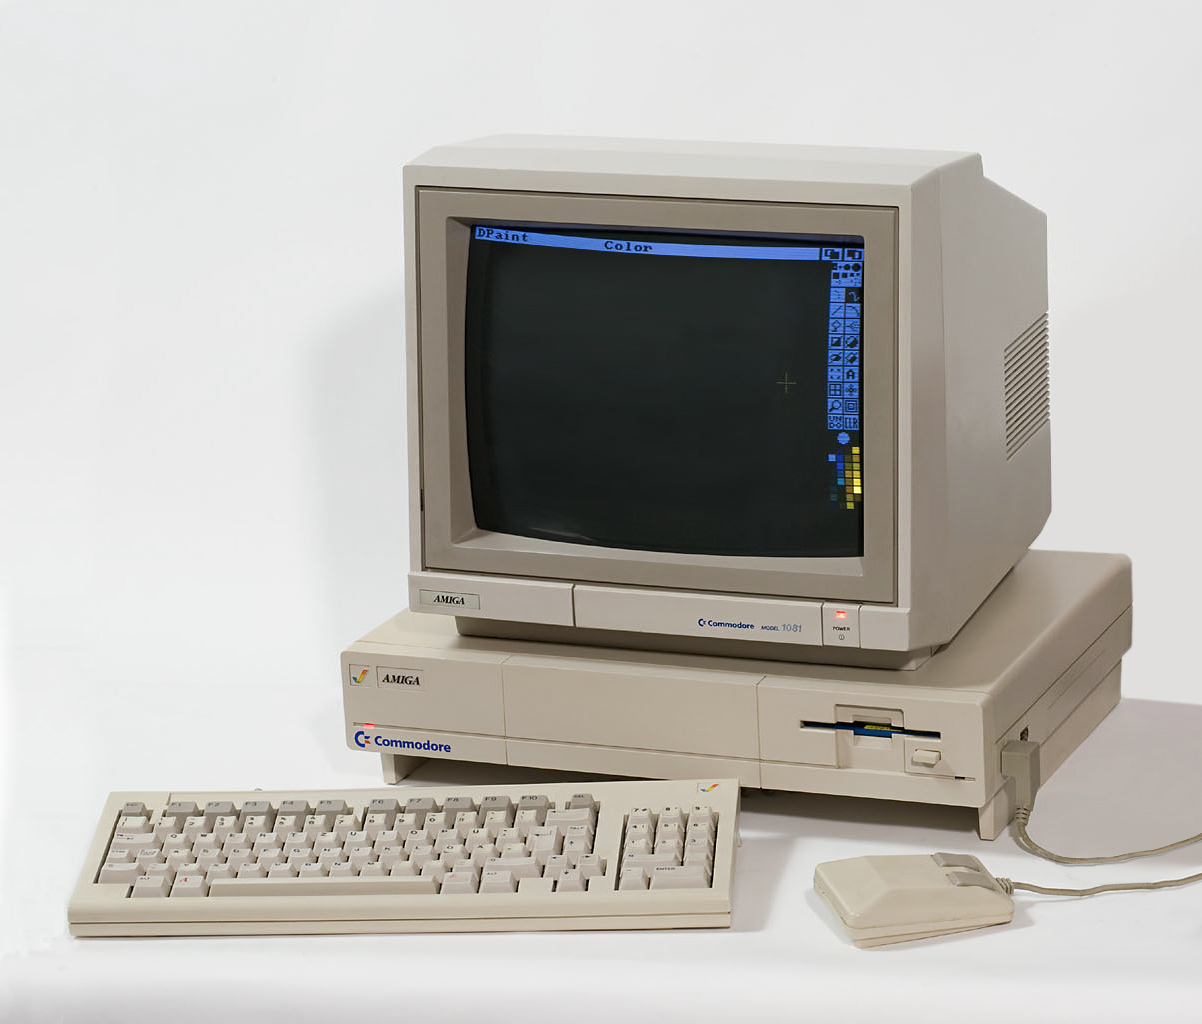
\includegraphics[width=\linewidth]{images/demoscene/amiga1000.png}
    \caption{Amiga 1000 - 1986}
    \label{am1000}
  \end{minipage}
  \hfill
  \begin{minipage}[b]{0.30\linewidth}
    \centering
    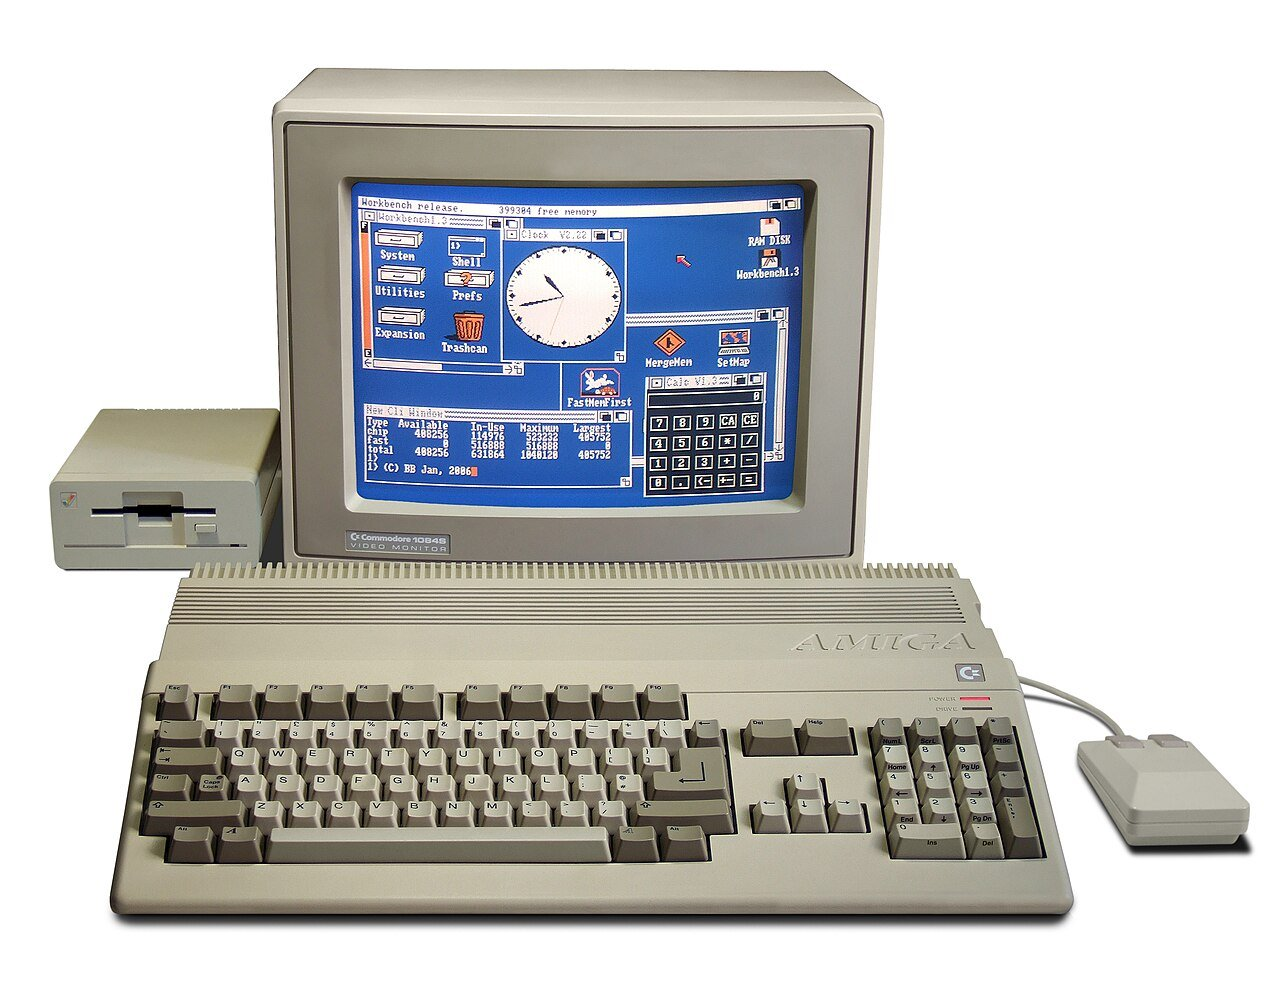
\includegraphics[width=\linewidth]{images/demoscene/amiga500.png}
    \caption{Amiga 500 - 1987}
    \label{am500}
  \end{minipage}
  \hfill
  \begin{minipage}[b]{0.30\linewidth}
    \centering
    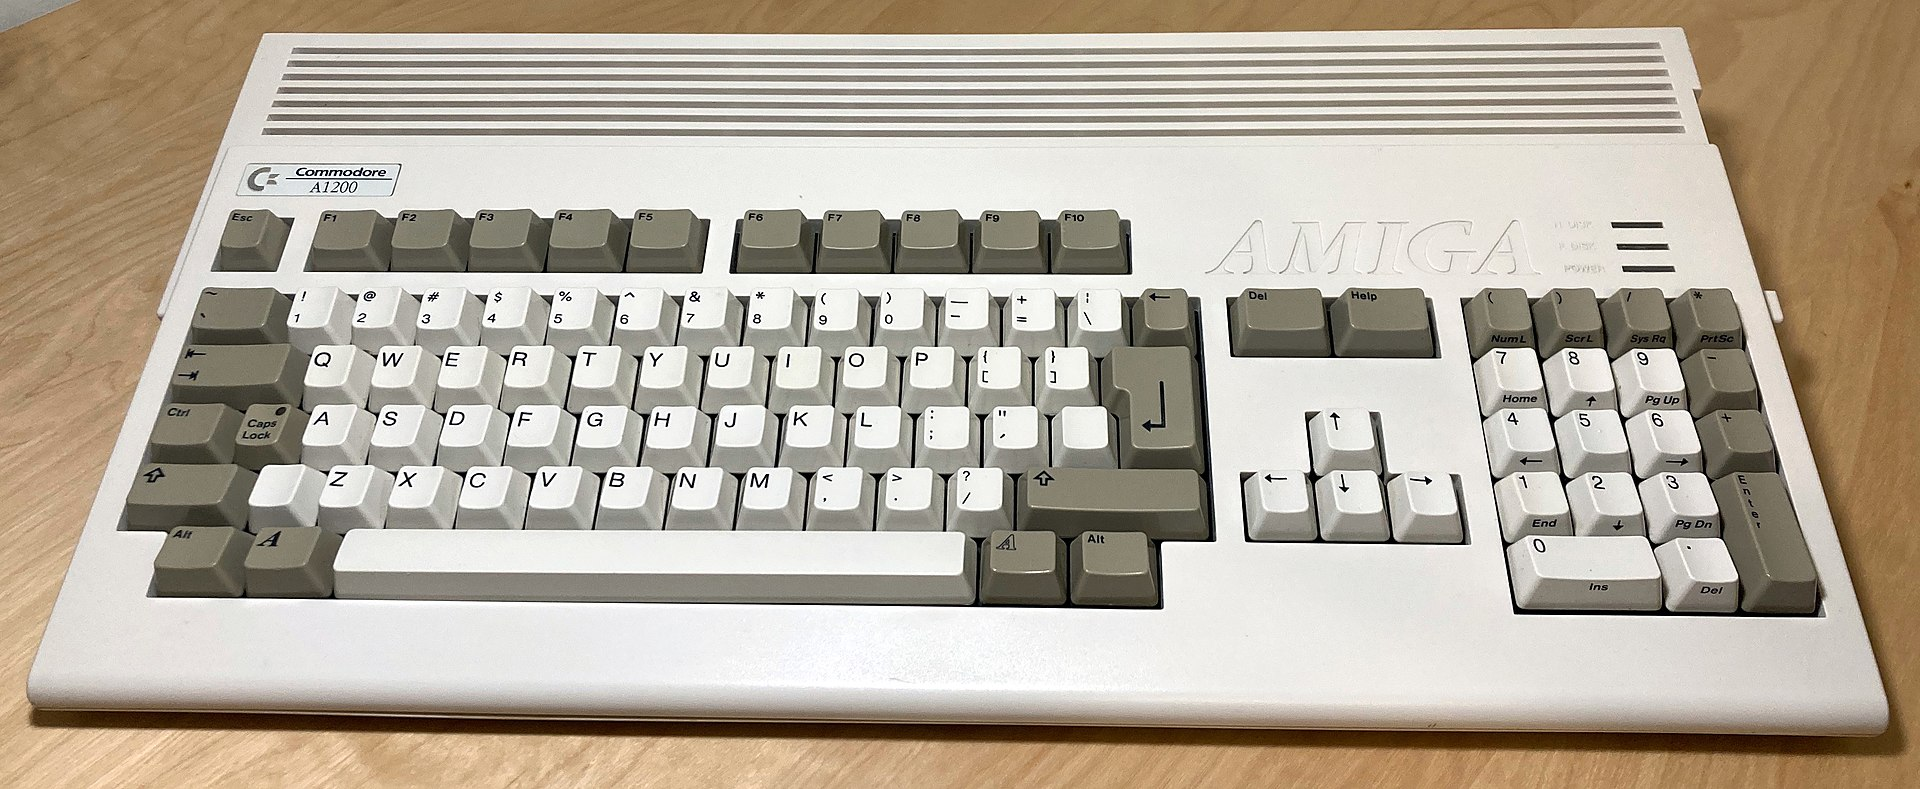
\includegraphics[width=\linewidth]{images/demoscene/amiga1200.png}
    \caption{Amiga 1200 - 1992}
    \label{am1200}
  \end{minipage}
  \label{chaos1}
\end{figure}

% Toutefois, une fois que la communauté a commencé à exploiter pleinement les capacités de l'Amiga, le paysage de la \textit{demoscene} a changé de manière spectaculaire. Des \textit{demos} emblématiques comme la « CHAOS Mega demo » ont vu le jour (voir \ref{chaos2}), illustrant les capacités multimédia avancées de la machine. Initialement centrés sur l'adaptation d'effets graphiques existants, les développeurs ont progressivement exploité le potentiel unique de l'Amiga, produisant des \textit{demos} de plus en plus complexes et impressionnantes.



L'introduction de l'Amiga a été un catalyseur pour la création d'une scène spécifique autour de cette plateforme. Elle a vu l'émergence de groupes dédiés, chacun avec ses spécialités : \textit{crackers} et \textit{demomakers}. Deux courants distincts se sont formés : l'un axé sur les programmes DOS\footnote{Un « programme DOS » ne se réfère pas au système d'exploitation MS-DOS que l'on trouve sur les PC, mais plutôt à un type de \textit{demo} spécifique conçu pour l'Amiga. Ces \textit{demos} étaient généralement exécutées à partir du Workbench, l'environnement graphique de l'Amiga, plutôt que de démarrer directement depuis un disque bootable.} et l'autre sur les \textit{trackloaders}\footnote{Un \textit{trackloader} désigne une technique de chargement de données utilisée pour produire des \textit{demos} plus fluides et interactives.}. 

Les programmes DOS sur Amiga étaient souvent caractérisés par une approche plus structurée et formelle, avec une présentation plus traditionnelle et un enchaînement linéaire des effets. A contrario, plutôt que de charger toutes les données nécessaires pour une \textit{demo} au début de l'exécution, le \textit{trackloader} charge les données progressivement à partir du disque pendant que la \textit{demo} est en cours d'exécution. Cette méthode permet d'offrir une expérience plus fluide et dynamique, car elle réduit les temps de chargement et permet un enchaînement plus naturel des effets et des scènes.



L'essor de l'Amiga a marqué un tournant dans la création musicale au sein de la \textit{demoscene}. Les premiers logiciels utilisés, appelés \textit{trackers}, rappellent les outils du C64 mais offraient la capacité de jouer des sons numérisés. Cette évolution a ouvert la porte à des compositions musicales plus complexes et sophistiquées, enrichissant ainsi la qualité sonore des \textit{demos}.

Aujourd'hui, les créateurs de \textit{demos} ont accès à des logiciels de production musicale plus avancés, les mêmes qui sont utilisés pour produire les morceaux diffusés à la radio ou en \textit{streaming}. Cependant, les contraintes de taille imposées par les \textit{demos} de 4 ou 64 Ko limitent l'utilisation de ces sons numérisés.

\subsection*{La synthèse sonore dans la \textit{demoscene}}

Face à ces limitations, les artistes reviennent souvent aux techniques ancestrales de la \textit{demoscene}. Ils créent des sons en partant de simples formes d'ondes, utilisant des méthodes de synthèse sonore pour générer des mélodies et des rythmes envoûtants. Ces approches minimalistes rappellent les débuts de la musique sur le C64, mais avec l'ingéniosité et l'expérience acquises au fil des années, les artistes parviennent à produire des compositions étonnamment riches et variées, démontrant ainsi que la créativité peut s'épanouir même dans les contraintes les plus strictes.


\begin{figure}[h]
  \begin{minipage}[b]{0.30\linewidth}
    \centering
    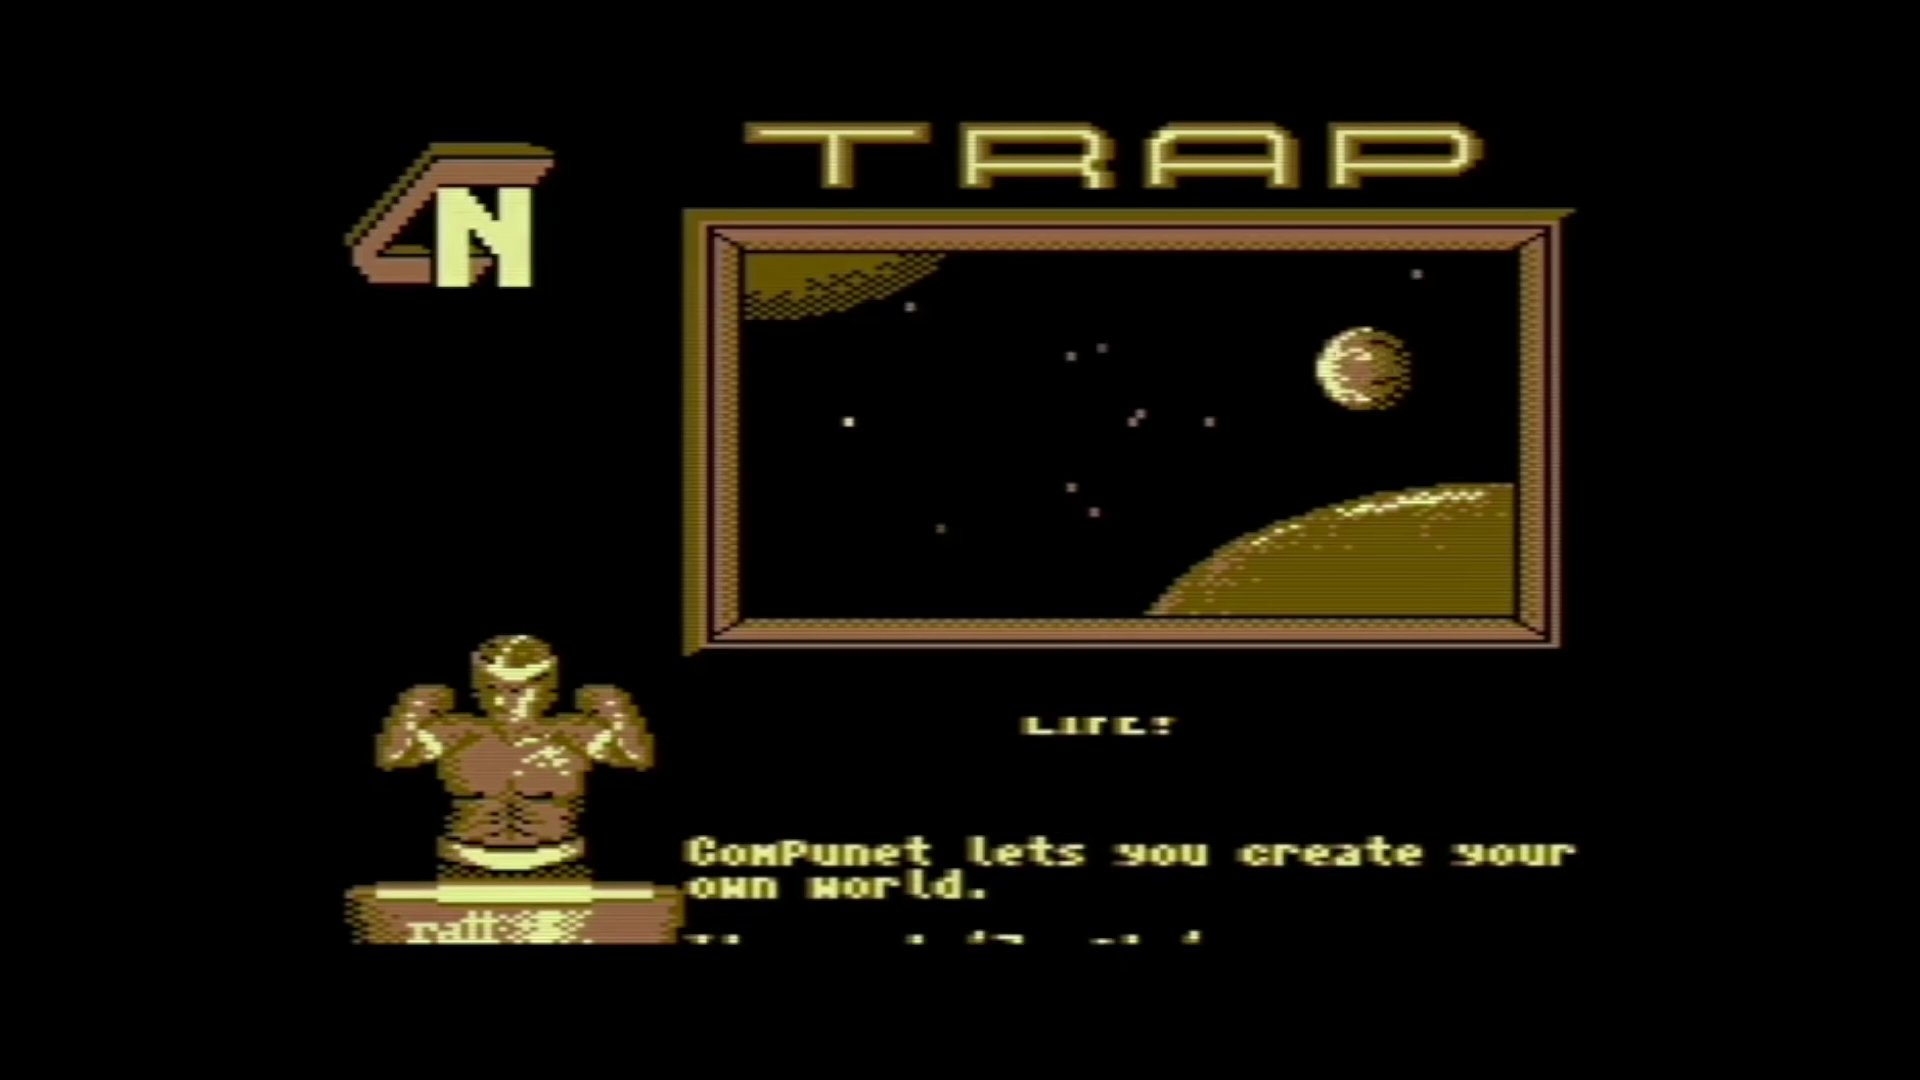
\includegraphics[width=\linewidth]{images/demoscene/demos/drumman1.png}
  \end{minipage}
  \hfill
  \begin{minipage}[b]{0.30\linewidth}
    \centering
    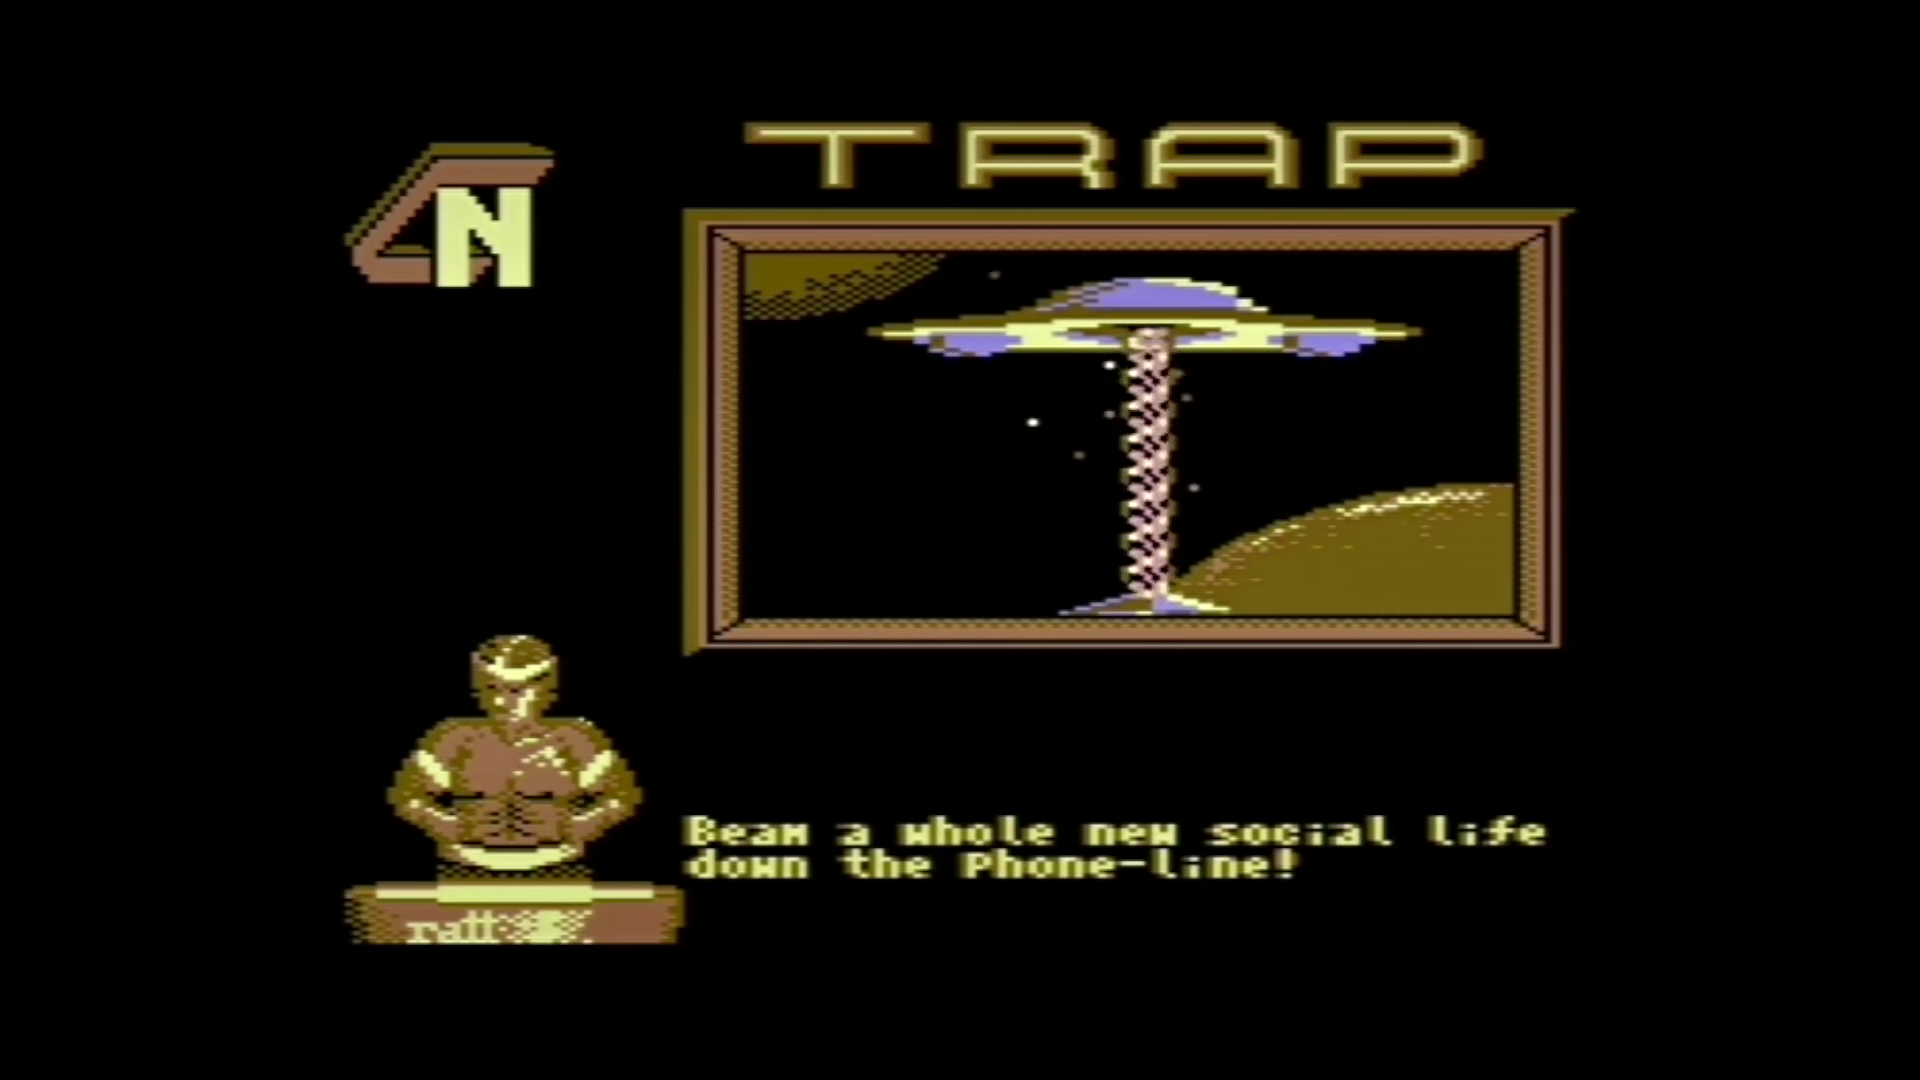
\includegraphics[width=\linewidth]{images/demoscene/demos/drumman2.png}
  \end{minipage}
  \hfill
  \begin{minipage}[b]{0.30\linewidth}
    \centering
    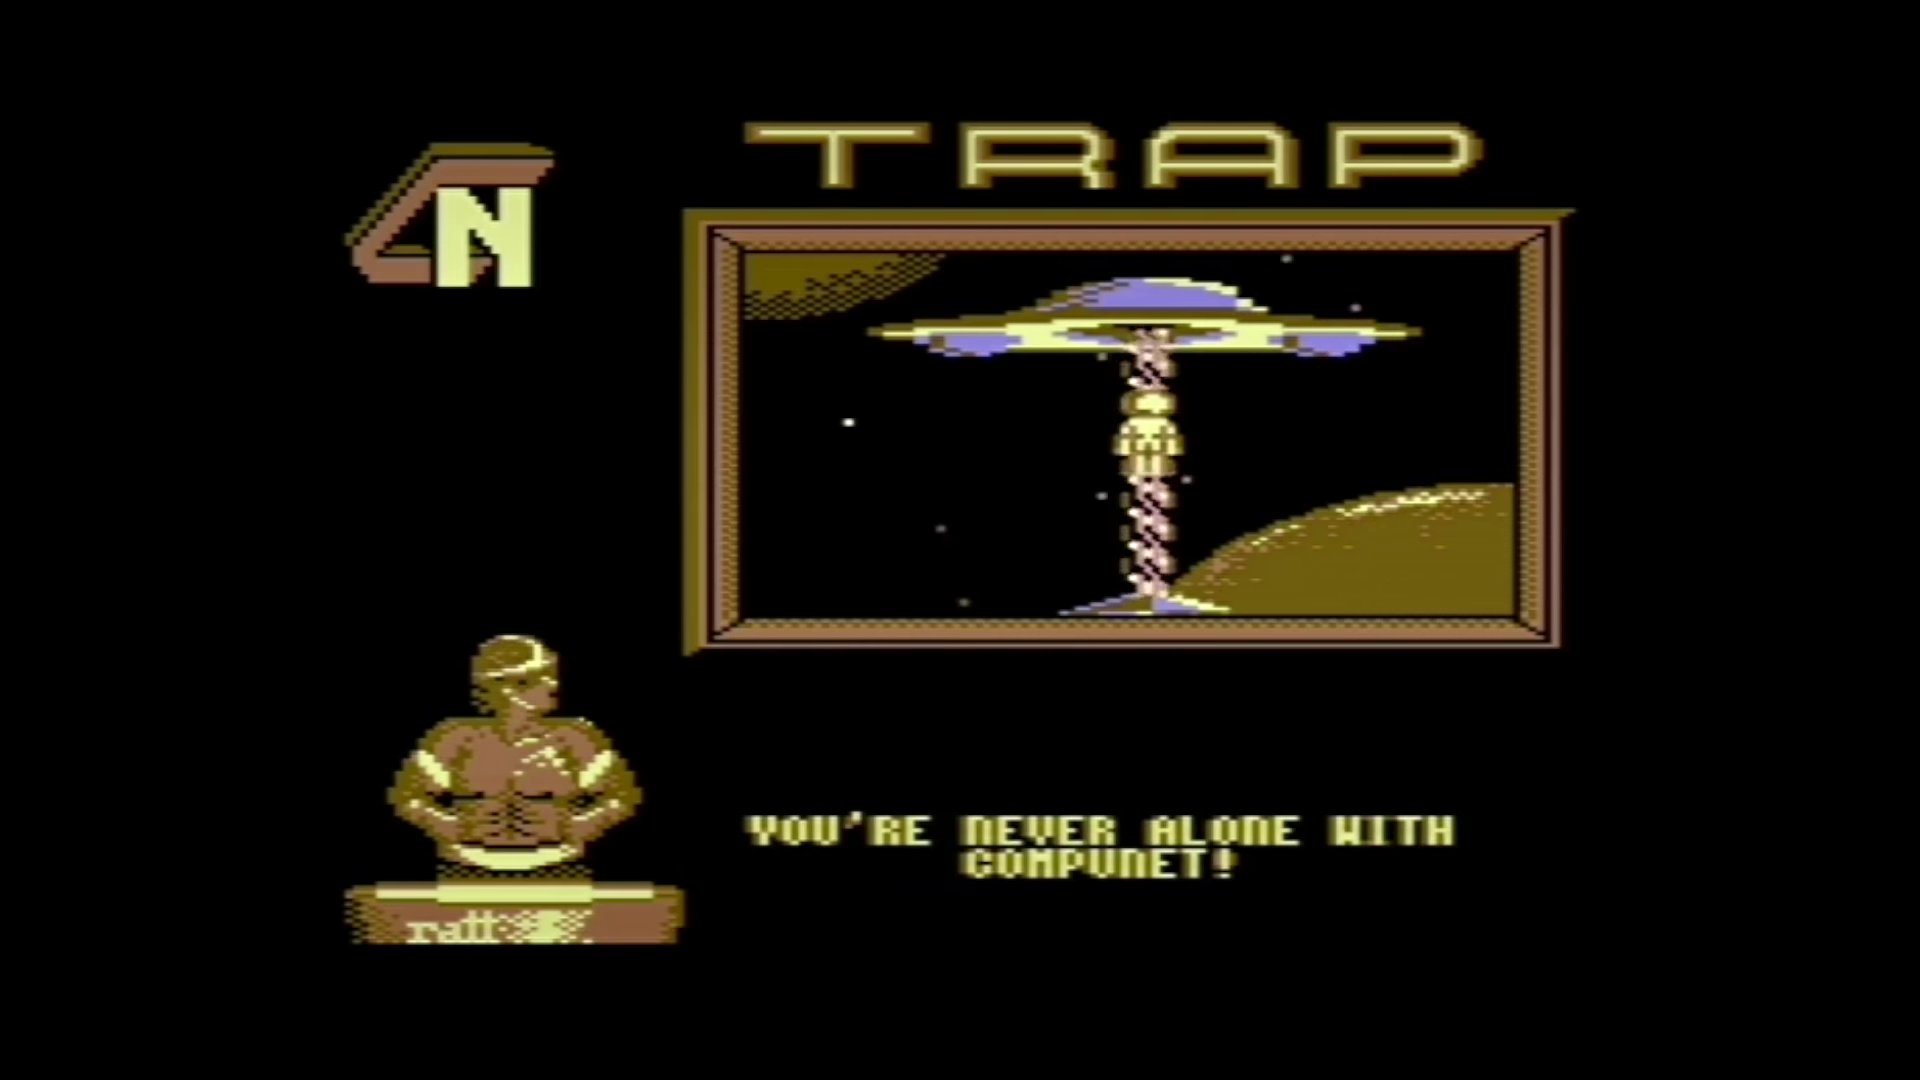
\includegraphics[width=\linewidth]{images/demoscene/demos/drumman3.png}
  \end{minipage}
  \caption{Drum Man Demo}
  \label{drumman}
\end{figure}



\subsection*{Les \textit{diskmags} confèrent à la scène une dimension plus structurée}

Les \textit{demos} Amiga ont élargi leurs horizons en incorporant des diaporamas, des albums musicaux et des \textit{diskmags}, se démarquant clairement par leur qualité supérieure par rapport aux \textit{diskmags} du C64. En plus des échanges directs entre individus, des médias physiques ont commencé à voir le jour pour soutenir et documenter la scène. 

\begin{figure}[h]
  \begin{minipage}[b]{0.45\linewidth}
    \centering
    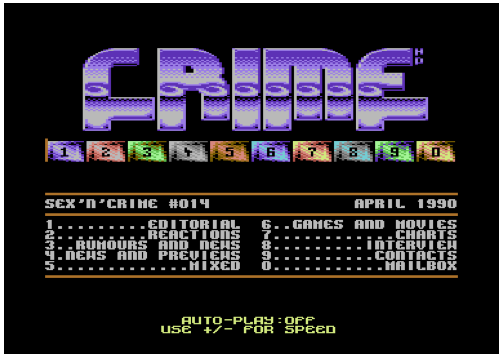
\includegraphics[width=\linewidth, height=1.5in]{images/demoscene/demos/diskmag1.png}
    \caption{Sex And Crime \#14, \textit{diskmag} sur disquette. (Commodore 64, 1990)}
    \label{diskmag1}
  \end{minipage}
  \hspace{0.1\linewidth} % Espace horizontal pour la gouttière
  \begin{minipage}[b]{0.45\linewidth}
    \centering
    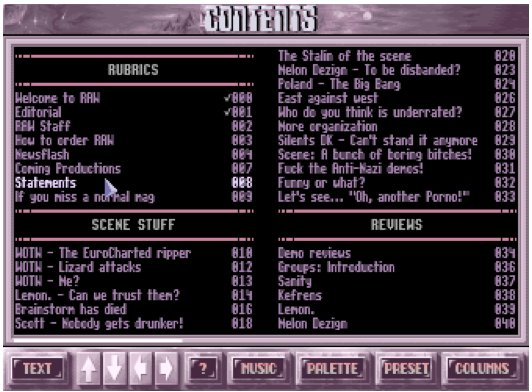
\includegraphics[width=\linewidth, height=1.5in]{images/demoscene/demos/diskmag2.png}
    \caption{R.A.W. \#6, un exemple de l'âge d'or des \textit{diskmags}. (Amiga 500, 1993)}
    \label{diskmag2}
  \end{minipage}
\end{figure}

Des magazines papier et des fanzines numériques ont été créés (les \textit{diskmags}\footnote{Les \textit{diskmags} sont des magazines numériques interactifs destinés à la communauté de la \textit{demoscene}. Ils sont généralement composés de plusieurs sections, y compris des articles, des critiques, des interviews, des classements, et parfois 
même des \textit{demos} ou des \textit{intros} intégrées.}), offrant un espace d'expression aux membres de la communauté et permettant de partager des actualités, des tutoriels, des critiques et des analyses (voir \ref{diskmag1}, \ref{diskmag1} et \ref{diskmagUI2}). 

\begin{figure}[h]
  \begin{minipage}[b]{0.30\linewidth}
    \centering
    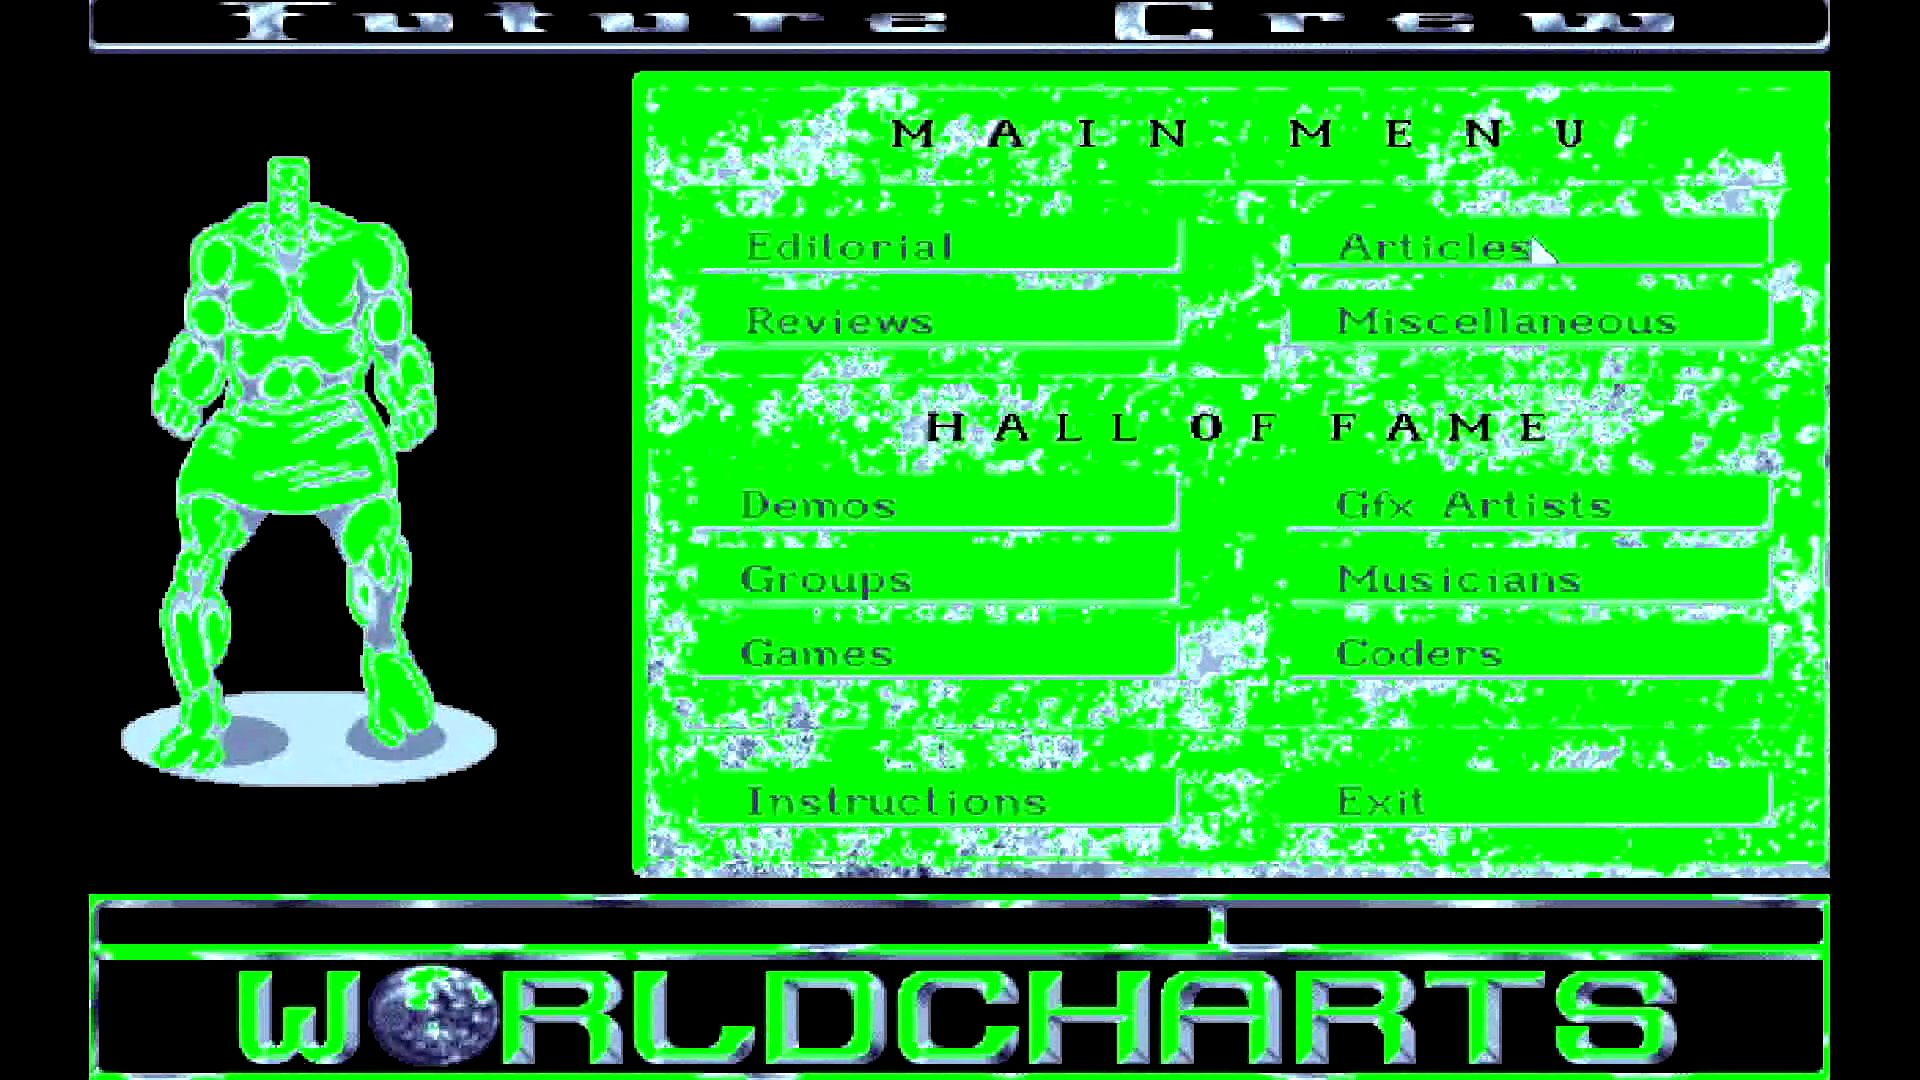
\includegraphics[width=\linewidth]{images/demoscene/demos/diskmag3.png}
  \end{minipage}
  \hfill
  \begin{minipage}[b]{0.30\linewidth}
    \centering
    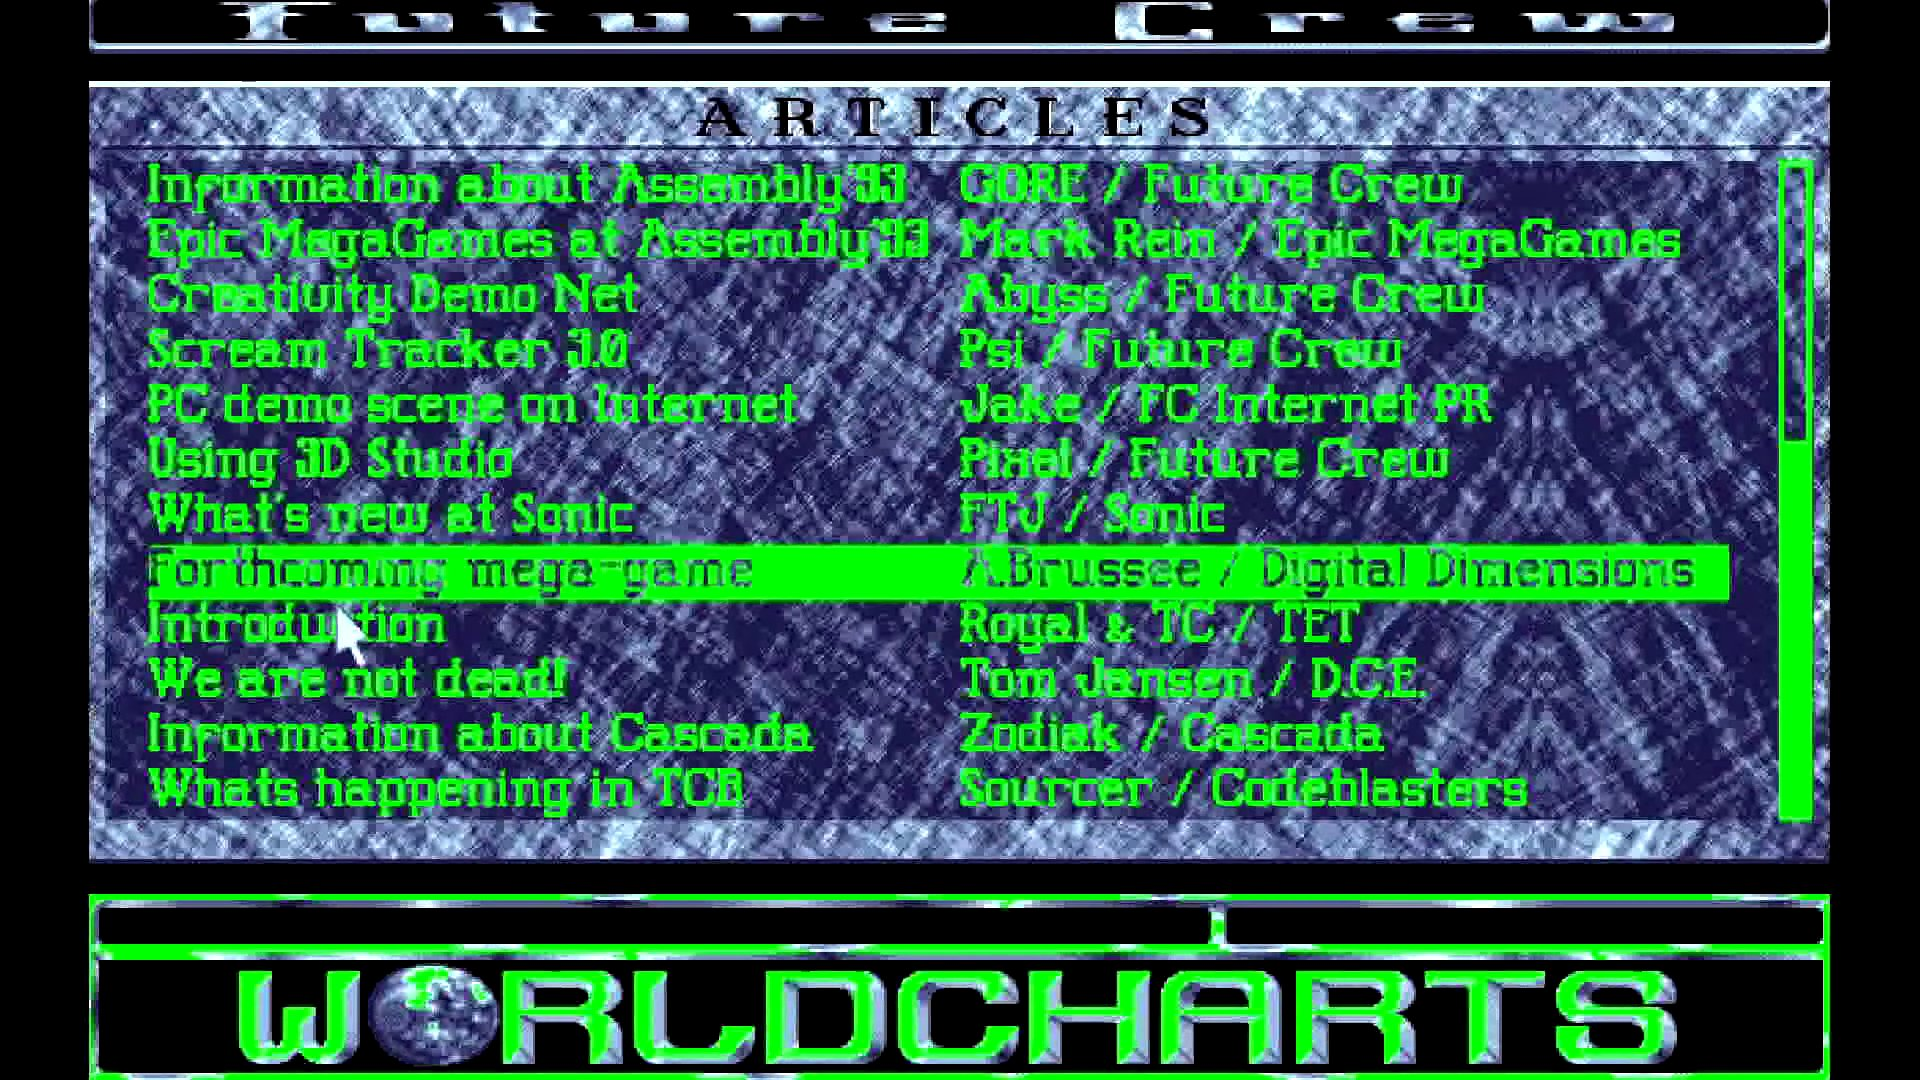
\includegraphics[width=\linewidth]{images/demoscene/demos/diskmag4.png}
  \end{minipage}
  \hfill
  \begin{minipage}[b]{0.30\linewidth}
    \centering
    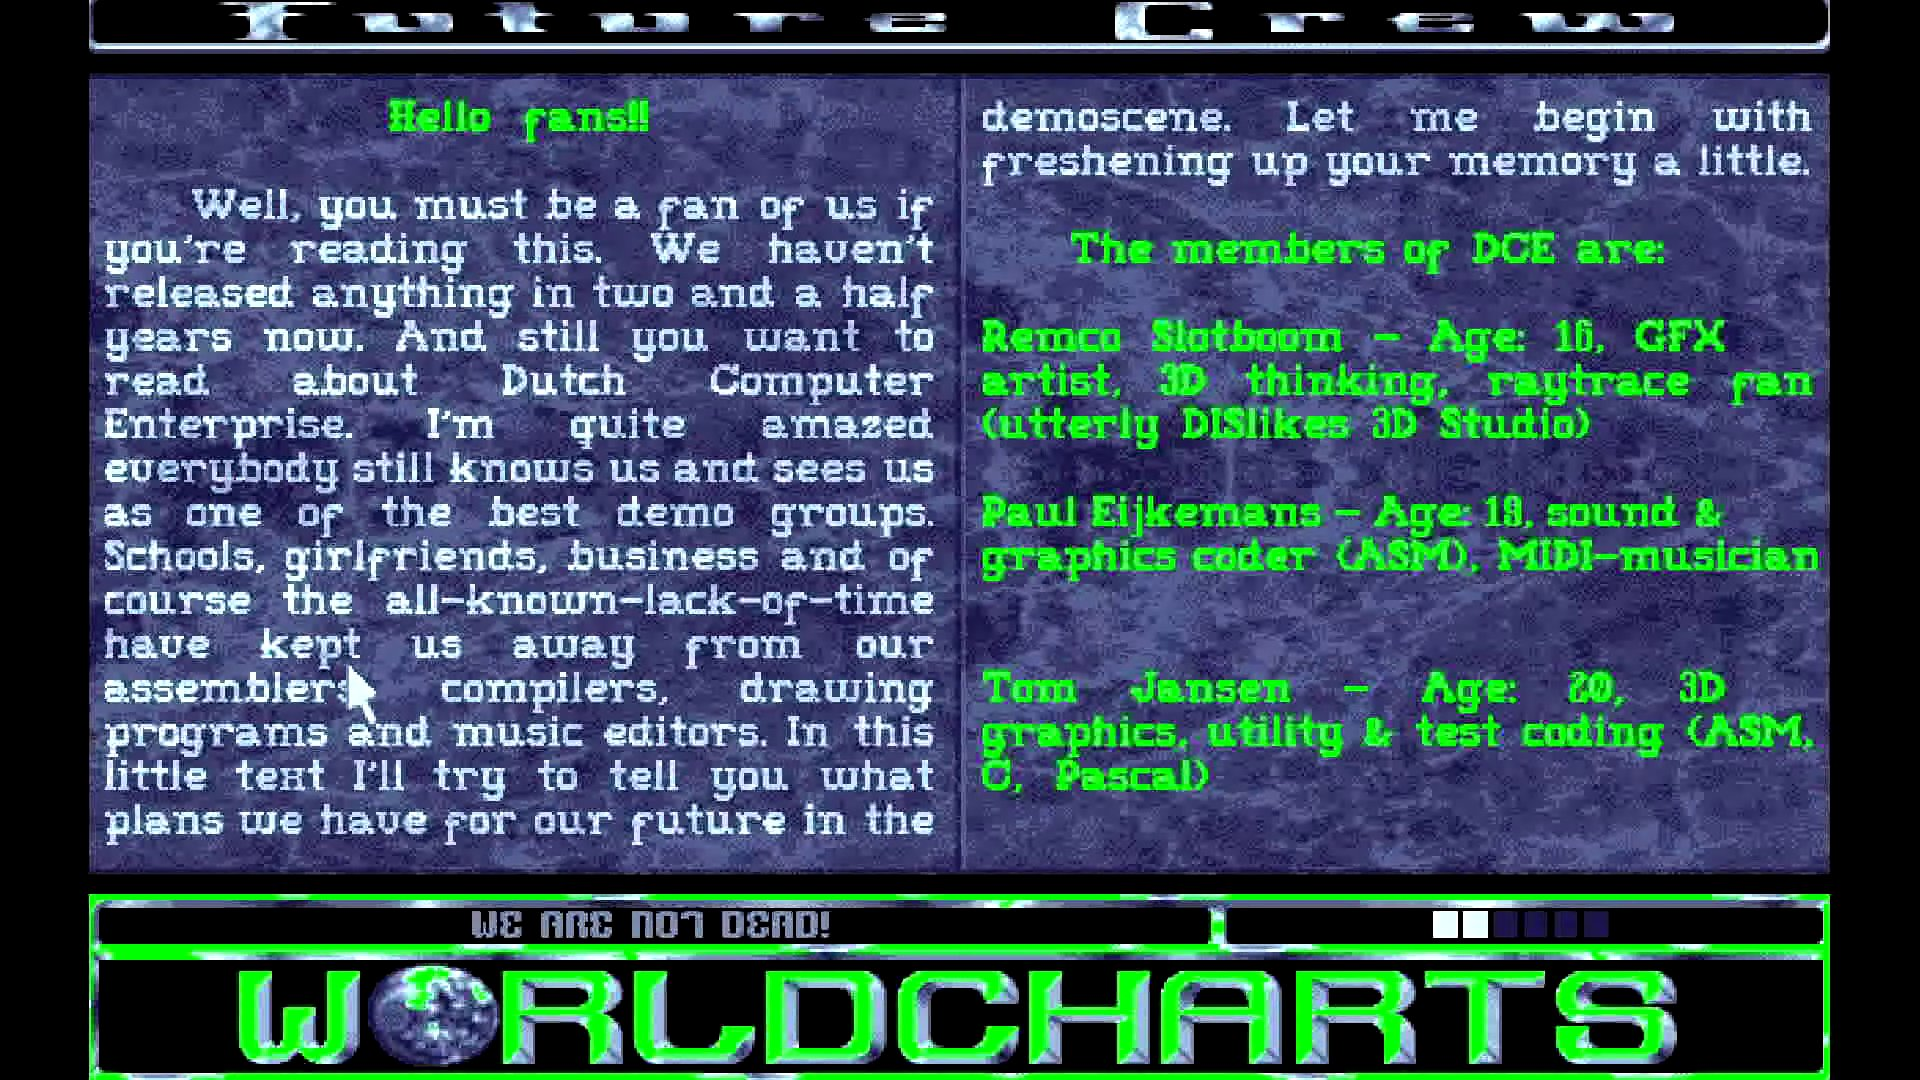
\includegraphics[width=\linewidth]{images/demoscene/demos/diskmag5.png}
  \end{minipage}
  \caption{Interface d'un diskmag}
  \label{diskmagUI2}
\end{figure}


Ces publications ont joué un rôle important dans la diffusion des idées et des valeurs de la \textit{demoscene} et du \textit{hacking}. Des titres comme Sex'n'Crime, Mamba et Fölény sont devenus emblématiques. Ces publications, enrichies de nouvelles, de critiques de \textit{demos}, de classements et d'informations sur les \textit{copyparties}, ont conféré à la scène une dimension plus structurée et sérieuse. 



% Des \textit{demos} emblématiques comme la « CHAOS Mega demo » ont vu le jour (voir \ref{chaos2}), illustrant les capacités multimédia avancées de la machine.

\subsection*{Compétition et prestige dans la \textit{demoscene}}

\begin{figure}[h]
  \begin{minipage}[b]{0.30\linewidth}
    \centering
    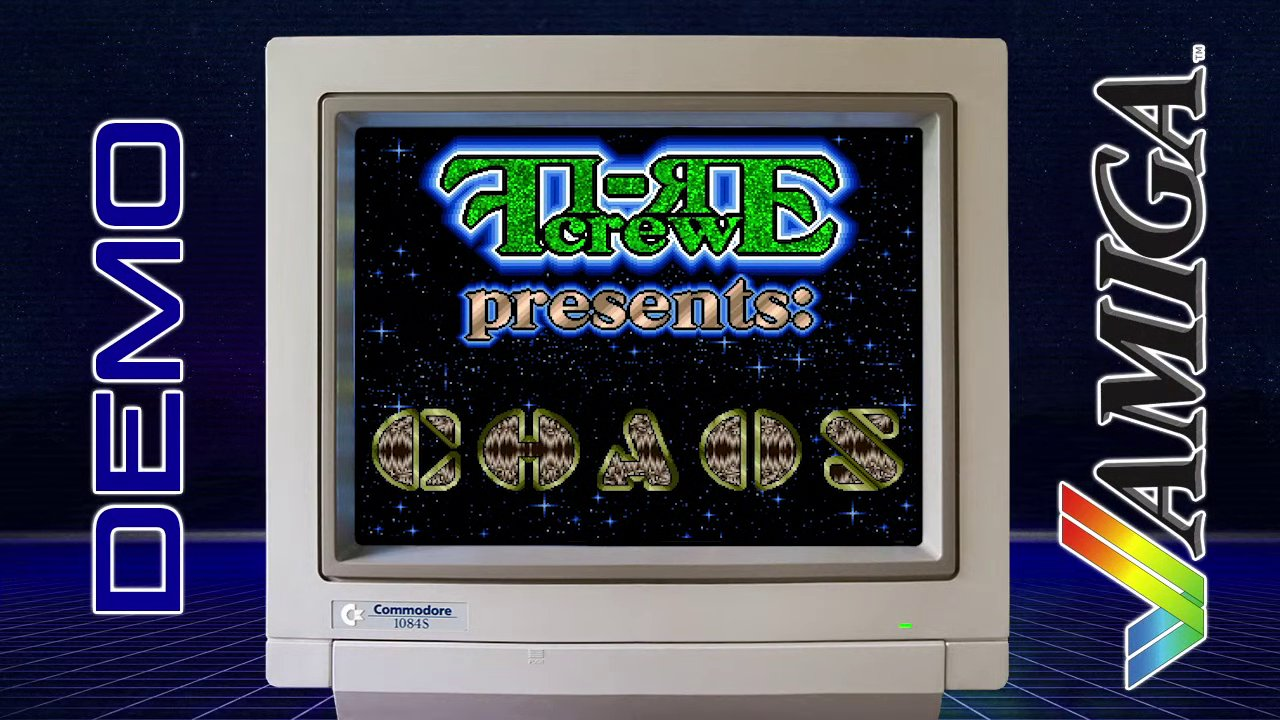
\includegraphics[width=\linewidth]{images/demoscene/demos/chaos1.png}
  \end{minipage}
  \hfill
  \begin{minipage}[b]{0.30\linewidth}
    \centering
    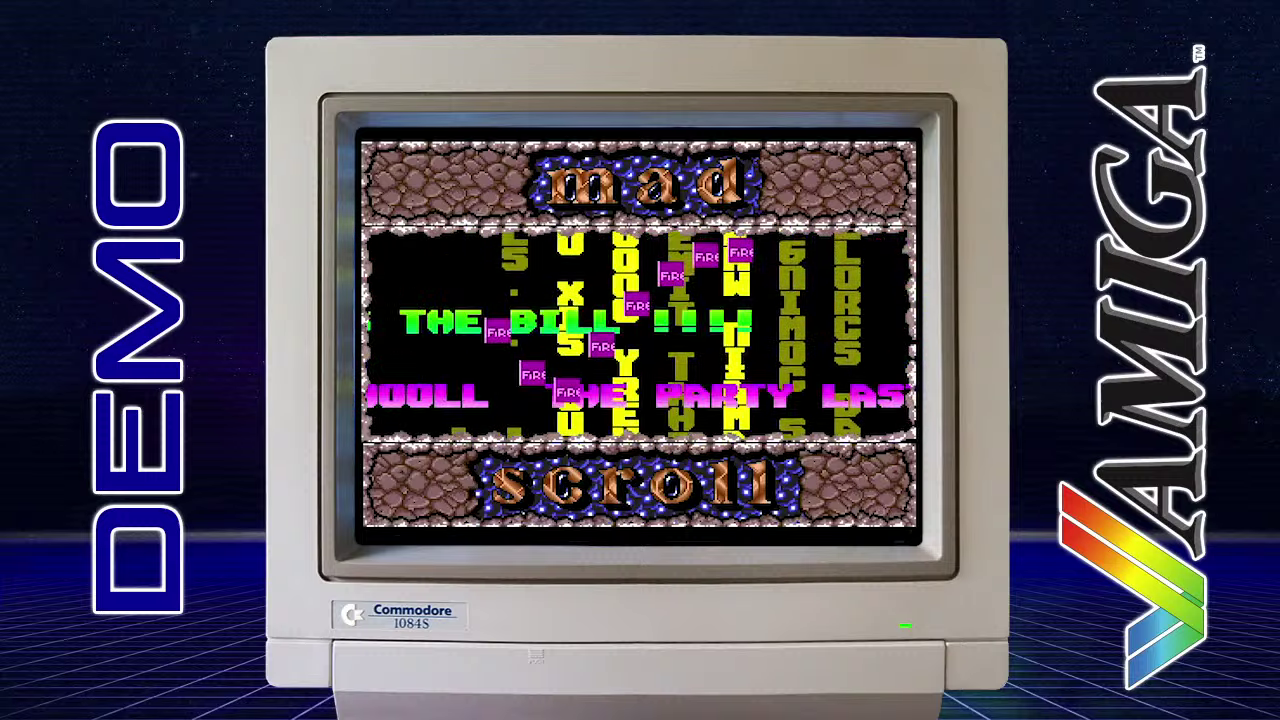
\includegraphics[width=\linewidth]{images/demoscene/demos/chaos2.png}
  \end{minipage}
  \hfill
  \begin{minipage}[b]{0.30\linewidth}
    \centering
    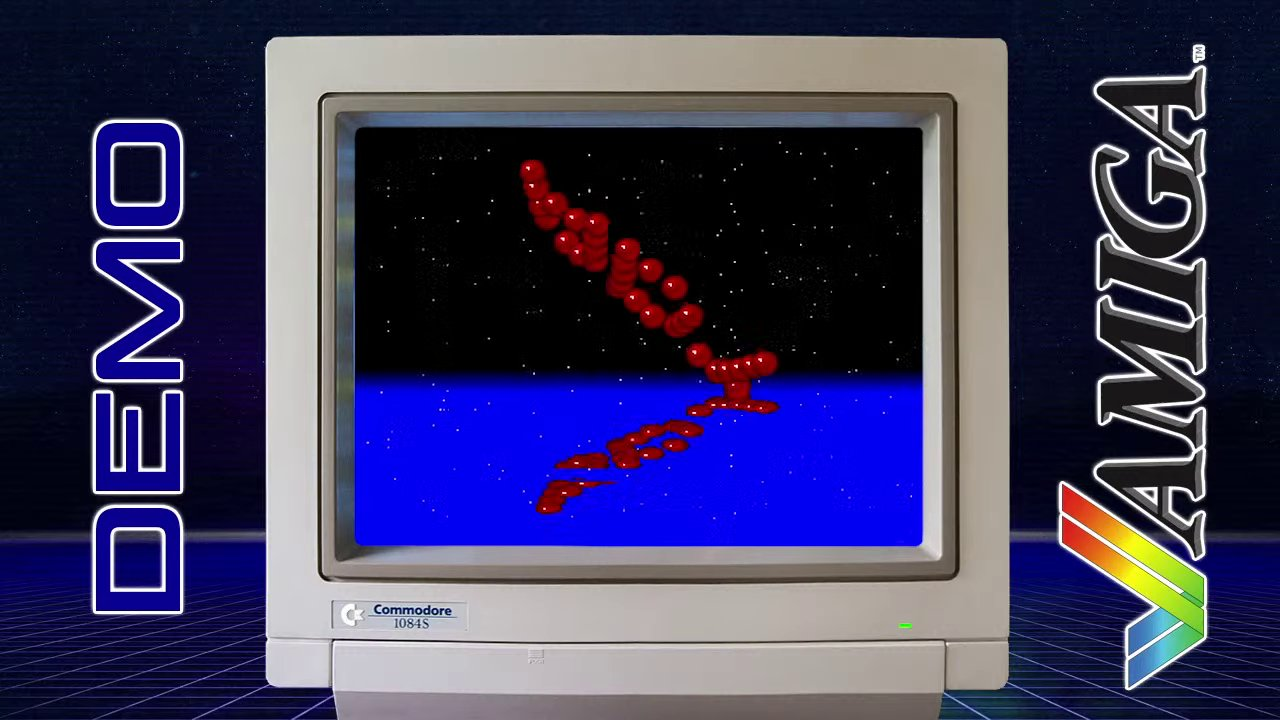
\includegraphics[width=\linewidth]{images/demoscene/demos/chaos3.png}
  \end{minipage}
  \caption{CHAOS Mega demo - Fi-Re Crew}
  \label{chaos2}
\end{figure}

C'est durant cette période qu'un véritable esprit compétitif a pris forme au sein de la communauté des \textit{demosceners}. Une course à l'exploit était engagée : qui serait le premier à pirater un jeu ? Qui concevrait l'\textit{intro} la plus marquante ? L'esprit de compétition a incité les créateurs à repousser les limites techniques de leurs machines. Les effets visuels se sont multipliés et complexifiés: animations de sprites, rotations, rebonds, effets de miroir, et bien d'autres encore. La musique n'était pas en reste, devenant de plus en plus sophistiquée.


Au-delà de la compétition purement technique, l'ego et le prestige ont également pris une place importante dans cet univers. Chaque groupe se devait de présenter un \textit{cracktro} de qualité, non seulement pour montrer leur expertise technique, mais aussi pour asseoir leur réputation au sein de la communauté.

\newpage
\section{Différents types de compétition}

% \todo{déplacer avant la liste des compétitions}
\subsection*{Introduction}
\begin{figure}[h]
  \begin{minipage}[b]{0.30\linewidth}
    \centering
    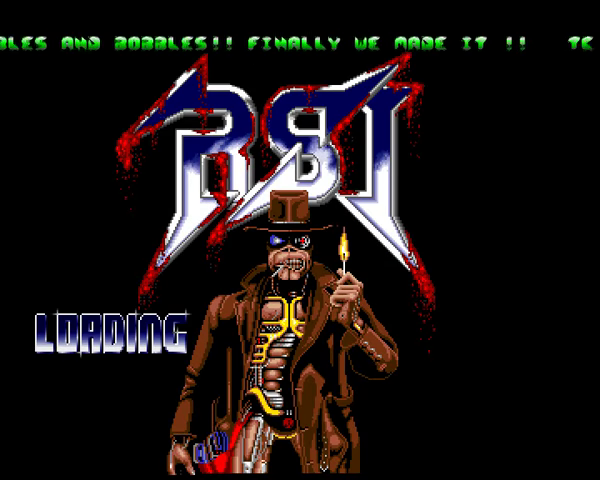
\includegraphics[width=\linewidth]{images/demoscene/demos/mega1.png}
  \end{minipage}
  \hfill
  \begin{minipage}[b]{0.30\linewidth}
    \centering
    
\includegraphics[width=\linewidth]{images/demoscene/demos/mega2.png}
  \end{minipage}
  \hfill
  \begin{minipage}[b]{0.30\linewidth}
    \centering
    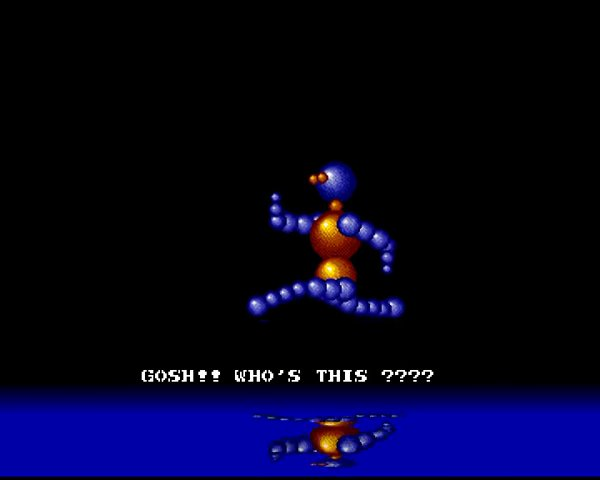
\includegraphics[width=\linewidth]{images/demoscene/demos/mega3.png}
  \end{minipage}
  \caption{Megademo - Red Sector Inc}
  \label{mega}
\end{figure}


La dimension communautaire joue un rôle tout aussi essentiel que le talent individuel dans la dynamique de la \textit{demoscene}, contribuant à nourrir un esprit créatif et collaboratif. L'événement phare de cette communauté est la \textit{demoparty}, une manifestation dédiée à la célébration de la culture informatique. Lors de ces rassemblements, les participants ont l'opportunité de mettre en lumière leurs compétences et créations, d'échanger des connaissances et des idées, et de rencontrer des individus animés par la même passion. Les œuvres produites y sont présentées dans diverses catégories et soumises à l'appréciation du public et des pairs, renforçant ainsi l'esprit de compétition et de camaraderie qui anime la \textit{demoscene}.

Concourir lors d'une \textit{demoparty} représente une expérience unique pour les \textit{demomakers}. C'est l'occasion de voir leur travail projeté sur un grand écran, sublimé par une bande sonore diffusée sur un système son de qualité, devant un auditoire attentif et passionné. Ce moment de partage et de reconnaissance collective est souvent source d'inspiration et de motivation pour les participants.




\begin{figure}[h]
  \begin{minipage}[b]{0.30\linewidth}
    \centering
    
\includegraphics[width=\linewidth]{images/demoscene/demos/prod1.png}
  \end{minipage}
  \hfill
  \begin{minipage}[b]{0.30\linewidth}
    \centering
    \includegraphics[width=\linewidth]{images/demoscene/demos/prod2.png}
  \end{minipage}
  \hfill
  \begin{minipage}[b]{0.30\linewidth}
    \centering
    \includegraphics[width=\linewidth]{images/demoscene/demos/prod3.png}
  \end{minipage}
  \caption{The Product - Farbrausch}
  \label{product}
\end{figure}


Cette course à l'innovation et à la créativité a contribué à faire de la \textit{demoscene} un mouvement dynamique et en constante évolution, où chaque nouvelle réalisation repousse un peu plus les frontières de ce qui est techniquement possible. Ce qui pouvait impressionner une année semblait déjà dépassé l'année suivante.  Cet esprit compétitif a conduit à la création de diverses catégories, chacune présentant ses propres contraintes spécifiques.

\subsection*{\textit{Intros} 4k : l'art de la compacité}

L'introduction de la catégorie 4k a marqué une étape significative dans l'évolution de la \textit{demoscene}. Contrairement aux productions plus volumineuses qui disposent de plusieurs mégaoctets pour exprimer leur vision artistique, les productions 4k se limitent à seulement 4 kilooctets de données. Cette contrainte sévère en taille a poussé les \textit{demosceners} à optimiser les possibilités de compression pour produire des œuvres imposantes malgré leur petite taille.

Malgré les contraintes, les \textit{demomakers} redoublent d'astuces pour y parvenir. Bien que les résultats soient souvent d'une qualité graphique médiocre, il est important de souligner que la taille de ces \textit{intros} est même inférieure à celle d'un document Word vide. Le format 4k a donc donné naissance à des \textit{demos} qui démontrent la puissance et le génie des \textit{demosceners}, en montrant qu'il est possible de réaliser des prouesses artistiques et techniques avec des ressources limitées.

\subsection*{« We Are New » par Fairlight}
Une des \textit{intros} 4k les plus célèbres sur Commodore 64 est « We Are New » par Fairlight (voir \ref{wnew}). Cette \textit{intro} a été saluée pour son ingéniosité technique et son esthétique, tout en tenant dans la contrainte de seulement 4~kilooctets de données.
\begin{figure}[h]
  \begin{minipage}[b]{0.30\linewidth}
    \centering
    \includegraphics[width=\linewidth]{images/demoscene/demos/wnew1.png}
  \end{minipage}
  \hfill
  \begin{minipage}[b]{0.30\linewidth}
    \centering
    \includegraphics[width=\linewidth]{images/demoscene/demos/wnew2.png}
  \end{minipage}
  \hfill
  \begin{minipage}[b]{0.30\linewidth}
    \centering
    \includegraphics[width=\linewidth]{images/demoscene/demos/wnew3.png}
  \end{minipage}
  \caption{« We Are New » - Fairlight}
  \label{wnew}
\end{figure}


\subsection*{L'\textit{Intro} 64k : un équilibre parfait entre créativité et optimisation}
Les \textit{intros} 64k occupent une place particulière dans la \textit{demoscene}, se positionnant entre les \textit{intros} 4k et les \textit{demos} \textit{full size}. Elles offrent une limite de 64~kilooctets de données, soit bien plus que les 4~kilooctets des \textit{intros} 4k, mais nettement moins que les \textit{demos} \textit{full size} qui peuvent s'étendre sur plusieurs mégaoctets.

Ici aussi, le défi des \textit{intros} 64k est de marier créativité artistique et optimisation technique dans un espace de stockage restreint. Ce format permet aux \textit{demosceners} de concevoir des œuvres plus élaborées, avec des graphismes, des effets sonores et des animations de qualité supérieure, tout en restant dans une taille de fichier modeste. L'objectif est là encore d'exploiter au maximum les 64 kilooctets disponibles.

L'\textit{intro} 64k se distingue par son système similaire aux \textit{intros} 4k, mais avec une limite étendue à 65535 octets. Ce format offre aux codeurs une plus grande marge de manœuvre créative, leur permettant de collaborer étroitement avec des graphistes et des musiciens pour créer des \textit{intros} marquantes. C'est pourquoi l'\textit{intro} 64k est l'une des catégories les plus appréciées des \textit{demomakers}, juste derrière la catégorie reine : la \textit{demo full size}.

\subsection*{« fr-08: .the .product » par Farbrausch}

Une des \textit{intros} 64k les plus célèbres et influentes dans la \textit{demoscene} est « fr-08: .the .product » réalisée par Farbrausch en 2000 (voir \ref{farb}). Cette \textit{intro} a marqué un tournant dans la catégorie des \textit{intros} 64k, démontrant une optimisation et une créativité jamais vues auparavant.

« fr-08: .the .product » a été distinguée non seulement pour ses effets visuels, mais aussi pour sa musique et sa synchronisation. Elle a repoussé les limites de ce qui était considéré comme possible dans un fichier de seulement 64~kilooctets, influençant de nombreux \textit{demomakers} et définissant de nouvelles normes pour les \textit{intros} 64k. Cette \textit{intro} est souvent citée comme un exemple de ce que la \textit{demoscene} peut réaliser.

\begin{figure}[h]
  \begin{minipage}[b]{0.30\linewidth}
    \centering
    \includegraphics[width=\linewidth]{images/demoscene/demos/farb1.png}
  \end{minipage}
  \hfill
  \begin{minipage}[b]{0.30\linewidth}
    \centering
    \includegraphics[width=\linewidth]{images/demoscene/demos/farb2.png}
  \end{minipage}
  \hfill
  \begin{minipage}[b]{0.30\linewidth}
    \centering
    \includegraphics[width=\linewidth]{images/demoscene/demos/farb3.png}
  \end{minipage}
  \caption{fr-08: .the .product - Farbrausch}
  \label{farb}
\end{figure}


\subsection*{Au-delà des contraintes : les \textit{demos full size}}


La catégorie \textit{demo full size} par ses productions les plus ambitieuses et les plus abouties , constitue le cœur battant de la \textit{demoscene}. À l'inverse des \textit{intros} 4k et 64k, soumises à des contraintes de taille de fichier plus strictes, les \textit{demos full size} se libèrent de toute limite prédéfinie en termes de mémoire ou de temps d'exécution.

Ce format offre aux \textit{demosceners} un espace de création illimité pour déployer tout leur talent et leur savoir-faire. Les \textit{demos full size} exploitent ainsi pleinement les capacités des machines sur lesquelles elles sont exécutées, que ce soit en termes de graphismes, d'animations, d'effets sonores ou de musique. Elles représentent souvent le résultat d'un travail d'équipe collaboratif, où artistes, codeurs, graphistes et musiciens fusionnent leurs compétences pour donner vie à une vision artistique commune.

Les productions de cette catégorie peuvent durer plusieurs minutes et offrent une expérience riche et immersive aux spectateurs. Elles peuvent raconter une histoire, présenter un univers visuel ou sonore unique, ou encore mettre en avant des techniques de programmation et de design nouvelles. La taille traditionnelle des \textit{demos} est limitée à 4Mo, bien que cette limite soit souvent dépassée, comme l'illustre la \textit{demo} de plus de 12Mo réalisée par Cocoon \& Syndrome pour « Shad » (voir \ref{shad}).

\begin{figure}[h]
  \begin{minipage}[b]{0.30\linewidth}
    \centering
    \includegraphics[width=\linewidth]{images/demoscene/demos/shad1.png}
  \end{minipage}
  \hfill
  \begin{minipage}[b]{0.30\linewidth}
    \centering
    \includegraphics[width=\linewidth]{images/demoscene/demos/shad2.png}
  \end{minipage}
  \hfill
  \begin{minipage}[b]{0.30\linewidth}
    \centering
    \includegraphics[width=\linewidth]{images/demoscene/demos/shad3.png}
  \end{minipage}
  \caption{Shad - Cocoon \& Syndrome}
  \label{shad}
\end{figure}



En somme, la catégorie \textit{demo full size} est le terrain de jeu privilégié des \textit{demosceners} pour exprimer leur créativité sans limites, repoussant constamment les frontières de l'art numérique et de la programmation, tout en offrant une liberté d'expression artistique inégalée.


\subsection*{L'art visuel au cœur de la \textit{demoscene} : la catégorie \textit{gfx}}

\begin{figure}[h]
  \begin{minipage}[b]{0.30\linewidth}
    \centering
    \includegraphics[width=\linewidth]{images/demoscene/demos/deities1.png}
  \end{minipage}
  \hfill
  \begin{minipage}[b]{0.30\linewidth}
    \centering
    \includegraphics[width=\linewidth]{images/demoscene/demos/deities2.png}
  \end{minipage}
  \hfill
  \begin{minipage}[b]{0.30\linewidth}
    \centering
    \includegraphics[width=\linewidth]{images/demoscene/demos/deities3.png}
  \end{minipage}
  \caption{Deities - MFX}
  \label{deities}
\end{figure}


La catégorie \textit{gfx} (\textit{graphics}) dans la \textit{demoscene} se centre sur la création graphique et artistique, mettant en lumière le talent des graphistes qui élaborent des œuvres visuelles pour les \textit{demos}, \textit{intros} et autres productions de la \textit{demoscene}. Pour exceller dans ce domaine, les graphistes doivent posséder une variété de compétences. Ils doivent maîtriser des logiciels de dessin et de retouche d'image, tout en ayant une compréhension approfondie des contraintes techniques propres à la \textit{demoscene}, telles que la gestion des palettes de couleurs et l'optimisation des tailles de fichiers.





Les productions \textit{gfx} peuvent prendre diverses formes, qu'il s'agisse d'images fixes, d'animations ou même de séquences vidéo. Elles sont souvent évaluées sur des critères tels que leur originalité, leur qualité artistique, leur technique et leur intégration harmonieuse dans la production globale. La catégorie \textit{gfx} est une catégorie permettant aux graphistes de la \textit{demoscene} de mettre en avant leur talent, de partager leur passion pour l'art graphique et de contribuer à enrichir les productions communautaires avec des visuels.



Cette catégorie \textit{gfx} est elle-même subdivisée en plusieurs sous-catégories, telles que les 8bits (256 couleurs) et les 32bits. Il est important de noter que l'utilisation de photos scannées est généralement mal vue, voire interdite.

% \missingfigure{exemples GFX}

\subsection*{La musique des \textit{pixels} : la catégorie \textit{mod} de la \textit{demoscene}}

\begin{figure}[h]
  \begin{minipage}[b]{0.30\linewidth}
    \centering
    \includegraphics[width=\linewidth]{images/demoscene/demos/ephi1.png}
  \end{minipage}
  \hfill
  \begin{minipage}[b]{0.30\linewidth}
    \centering
    \includegraphics[width=\linewidth]{images/demoscene/demos/ephi2.png}
  \end{minipage}
  \hfill
  \begin{minipage}[b]{0.30\linewidth}
    \centering
    \includegraphics[width=\linewidth]{images/demoscene/demos/ephi3.png}
  \end{minipage}
  \caption{Ephidrena - Concrete}
  \label{ephi}
\end{figure}


La catégorie \textit{mod} (module) dans la \textit{demoscene} est dédiée à la création de musique et de sons, qui sont essentiels pour enrichir l'expérience audio des \textit{demos} ou des \textit{intros}. Les modules sont des fichiers spéciaux contenant à la fois des données musicales et des instructions pour les instruments, permettant ainsi de reproduire des compositions musicales variées. Ces créations sont le résultat du travail des musiciens et \textit{sound designers} de la \textit{demoscene} qui utilisent des \textit{trackers}\footnote{Le fonctionnement d'un \textit{tracker} est basé sur une interface de suivi de partitions, où chaque piste représente un instrument ou un échantillon. Les utilisateurs peuvent placer des notes, définir des effets et ajuster divers paramètres pour chaque piste à l'aide d'un clavier ou d'une interface graphique.}, des logiciels spécifiques à la \textit{demoscene}, pour composer leurs morceaux.

Les compétences nécessaires pour exceller dans cette catégorie sont nombreuses et incluent une connaissance approfondie des principes de la composition musicale, ainsi qu'une maîtrise des techniques spécifiques à la création de \textit{mods}. Parmi ces techniques, l'utilisation des \textit{trackers} et la manipulation des échantillons sonores sont particulièrement importantes. Les \textit{mods} peuvent varier grandement en style et en genre, allant de la musique électronique à la musique classique, en passant par le \textit{rock}, le \textit{jazz} et bien d'autres. Ils sont évalués sur des critères tels que leur originalité, leur qualité musicale, leur technique et leur intégration dans la production globale.



Autrefois, cette catégorie comprenait des compétitions Modules 4 voies et \textit{multichannels}, mais elle a évolué avec l'arrivée du format MP3, qui a en grande partie remplacé les compétitions traditionnelles. Le concept des modules, initialement développé par les \textit{demomakers} sur Atari et porté sur diverses plateformes comme l'Amiga, le PC ou l'Amstrad, est fondé sur l'enregistrement de petits sons pour composer une partition. Des logiciels comme FastTracker2 ou Scream Tracker sont utilisés pour créer ces partitions en manipulant les sons enregistrés à différentes vitesses pour reproduire les notes musicales (voir \ref{fasttracker00} et \ref{screamtracker00}). Certains musiciens de la \textit{demoscene}, tels que Skaven, Clawz et Necro, sont reconnus comme des références dans cet art.

\begin{figure}[h]
  \begin{minipage}[b]{0.45\linewidth}
    \centering
    \includegraphics[width=\linewidth, height=1.5in]{images/demoscene/fasttracker00.png}
    \caption{FastTracker 2}
    \label{fasttracker00}
  \end{minipage}
  \hspace{0.1\linewidth} % Espace horizontal pour la gouttière
  \begin{minipage}[b]{0.45\linewidth}
    \centering
    \includegraphics[width=\linewidth, height=1.5in]{images/demoscene/screamtracker00.png}
    \caption{Scream Tracker}
    \label{screamtracker00}
  \end{minipage}
\end{figure}


Dans les compétitions, les modules 4 voies permettent de jouer jusqu'à 4 instruments simultanément, tandis que les \textit{multichannels} offrent une plus grande capacité, souvent limitée à 32 ou 64 portées. Cette catégorie \textit{mod} offre ainsi une plateforme aux musiciens et \textit{sound designers} de la \textit{demoscene} pour exprimer leur talent, partager leur passion pour la musique et contribuer à enrichir les productions de la communauté \textit{demoscene} avec des compositions audio.



% \missingfigure{illustration de la catégorie mod}

\subsection*{Au-delà des frontières : la catégorie \textit{wild}}

\begin{figure}[h]
  \begin{minipage}[b]{0.30\linewidth}
    \centering
    \includegraphics[width=\linewidth]{images/demoscene/demos/futur1.png}
  \end{minipage}
  \hfill
  \begin{minipage}[b]{0.30\linewidth}
    \centering
    \includegraphics[width=\linewidth]{images/demoscene/demos/futur2.png}
  \end{minipage}
  \hfill
  \begin{minipage}[b]{0.30\linewidth}
    \centering
    \includegraphics[width=\linewidth]{images/demoscene/demos/futur3.png}
  \end{minipage}
  \caption{Future Crew - Second Reality}
  \label{sreal}
\end{figure}


Au fil du temps, l'évolution de la \textit{demoscene} a engendré l'émergence de formes artistiques nouvelles, difficiles à catégoriser au sein des catégories traditionnelles comme la musique, les images ou les \textit{demos}. De cette évolution est née la catégorie \textit{wild}, qui s'est imposée comme un terrain d'expression artistique non conventionnel.

Les concours \textit{wild} offrent souvent des spectacles en direct où les créateurs montent sur scène pour dévoiler leurs œuvres. Ces présentations peuvent varier d'un microcontrôleur récupéré d'un réfrigérateur à des performances artistiques plus extravagantes. Malgré leur caractère parfois déconcertant, ces productions sont généralement le fruit d'un travail sérieux et méticuleux, combinant effets visuels et compositions musicales.





Aucune machine, aussi insolite soit-elle, n'échappe à l'exploration artistique de la \textit{demoscene}. De la simple calculatrice de poche aux installations monumentales, tout peut être utilisé comme vecteur d'expression artistique, reflétant ainsi la diversité de la communauté.

% \missingfigure{image catégorie wild}




% \paragraph{Avènement du PC}

% L'avènement du PC a introduit une nouvelle dimension dans le paysage des \textit{demos}. Toutefois, la diversité des configurations PC a constitué un défi majeur pour les développeurs. Malgré cela, les \textit{demos} PC ont progressé au fil du temps, mais l'influence de l'Amiga et du C64 demeure prépondérante.
\section{Techniques visuelles dans la \textit{demoscene}}

\begin{figure}[h]
  \begin{minipage}[b]{0.30\linewidth}
    \centering
    \includegraphics[width=\linewidth]{images/demoscene/demos/futur4.png}
  \end{minipage}
  \hfill
  \begin{minipage}[b]{0.30\linewidth}
    \centering
    \includegraphics[width=\linewidth]{images/demoscene/demos/futur5.png}
  \end{minipage}
  \hfill
  \begin{minipage}[b]{0.30\linewidth}
    \centering
    \includegraphics[width=\linewidth]{images/demoscene/demos/futur6.png}
  \end{minipage}
  \caption{Future Crew - Panic}
  \label{panic}
\end{figure}


Nous allons maintenant étudier quelques techniques fréquemment utilisées afin d'appréhender leur impact visuel. Parmi les méthodes adoptées par les \textit{demosceners} pour leurs créations, nous avons précédemment mentionné l'usage de la programmation en assembleur par les \textit{crackers} pour optimiser à la fois les performances et la taille des \textit{demos}. De plus, sur le Commodore 64, des fonctionnalités \textit{hardware} souvent méconnues ont été découvertes par les programmeurs astucieux de la \textit{demoscene}. Parmi ces trouvailles, on peut citer la capacité à éliminer la bordure de l'écran grâce aux \textit{raster interrupts}, ou encore l'utilisation d'un quatrième canal pour le son.

\subsection*{Synchronisation visuelle: les \textit{raster interrupts}}

Les \textit{raster interrupts} sont une technique utilisée dans la \textit{demoscene}, notamment sur le Commodore 64, pour synchroniser des effets visuels avec le balayage de l'écran (\textit{raster}). Le Commodore 64, comme de nombreux autres ordinateurs de cette époque, utilise un balayage \textit{raster} pour afficher les images à l'écran, c'est-à-dire qu'il dessine l'écran ligne par ligne, de haut en bas. Un \textit{raster interrupt} intervient lorsqu'un programme interrompt le processus normal de balayage \textit{raster} pour exécuter un code spécifique.

Dans la \textit{demoscene}, les \textit{raster interrupts} sont souvent utilisés pour créer des effets graphiques avancés, comme des \textit{rasterbars}, des effets de \textit{scrolling} et d'autres animations complexes comme le \textit{waving}.

\subsection*{Dépasser les limites de la palette}
Bien que le Commodore 64 puisse afficher seulement 16 couleurs dont seulement cinq nuances de gris, y compris le noir et le blanc, certaines \textit{demos} parvenaient à afficher plus de couleurs que cette palette de base. Une méthode pour y parvenir est d'alterner rapidement entre deux écrans légèrement différents pour mélanger les couleurs, exploitant la persistance rétinienne\footnote{La persistance rétinienne fait référence à la capacité de l'œil humain à percevoir une image pendant un court laps de temps après que l'image originale ait disparu. Cette caractéristique est exploitée dans la création de \textit{demos} pour produire des effets visuels fluides et dynamiques, en utilisant des techniques telles que le changement rapide d'images ou la manipulation de la luminosité et des couleurs.}. Cette technique est exposée dans « Dream Time » du groupe Profik, où deux buffers sont alternés 60 fois par seconde pour créer l'illusion de couleurs supplémentaires.

\subsection*{Les variations avancées du \textit{scroll}}
Un \textit{scroll} fait référence à une technique où le texte ou les graphiques défilent horizontalement ou verticalement à l'écran. Cette technique était largement utilisée pour afficher des crédits, des messages ou des graphismes artistiques dans les \textit{demos} et les \textit{intros}.
Initialement simples textes défilants, ils ont évolué vers des versions DYPP (\textit{Different	Y Pixel	Position}) ondulantes, des \textit{stretch-scrollers} irréguliers, des \textit{scrollers} inspirés de Star Wars, ou encore des \textit{scrollers} en 3D virtuelle autour d'une sphère.

\subsection*{Vagues et ondulations à l'écran: le \textit{waving}}
Le \textit{waving} désigne un effet graphique simulant des vagues ou des ondulations sur l'écran. Cet effet est souvent obtenu en manipulant les \textit{pixels} ou en modifiant les lignes de balayage de manière à créer une illusion de mouvement fluide et ondulant.

\subsection*{Maîtriser les lignes de balayage: le \textit{rasterbar}}
Un \textit{rasterbar} fait référence à un effet visuel créé en manipulant les lignes de balayage (\textit{rasters}) de l'écran. L'effet est généralement réalisé en changeant dynamiquement la couleur ou la luminosité des lignes de balayage pour créer des motifs ou des animations. Ces effets exploitent les caractéristiques techniques des anciens ordinateurs, comme le Commodore 64, qui permettaient un contrôle précis des lignes de balayage.




\subsection*{Simuler le mouvement: le \textit{bouncing}}
\textit{Bouncing} fait référence à un effet visuel où un objet ou du texte semble rebondir de haut en bas ou de gauche à droite à l'écran. Cet effet est souvent utilisé pour ajouter du dynamisme et de l'animation à une \textit{demo} ou à une \textit{intro}, donnant ainsi une sensation de mouvement et d'interaction.

\subsection*{Le \textit{logo} dans la \textit{demoscene} comme signature artistique}
Un \textit{logo} désigne généralement un élément graphique représentant le nom ou l'identité visuelle d'un groupe de \textit{demosceners}. Ce \textit{logo} est souvent intégré dans les \textit{intros}, les \textit{demos} ou les \textit{cracktros} pour identifier le groupe ou le collectif derrière la production. Il est conçu pour être distinctif et mémorisable, reflétant souvent le style et l'esthétique du groupe.

\begin{figure}[h]
  \begin{minipage}[b]{0.30\linewidth}
    \centering
    \includegraphics[width=\linewidth]{images/demoscene/demos/lemon1.png}
  \end{minipage}
  \hfill
  \begin{minipage}[b]{0.30\linewidth}
    \centering
    \includegraphics[width=\linewidth]{images/demoscene/demos/lemon2.png}
  \end{minipage}
  \hfill
  \begin{minipage}[b]{0.30\linewidth}
    \centering
    \includegraphics[width=\linewidth]{images/demoscene/demos/lemon3.png}
  \end{minipage}
  \caption{Lemonade - Fairlight}
  \label{lemon}
\end{figure}




% Aspect social de la \textit{demoscene}
\chapter{La \textit{demoscene} aujourd'hui}

\section{Fascination pour les machines emblématiques}

La \textit{demoscene} d'aujourd'hui est marquée par l'usage persistant d'ordinateurs obsolètes tels que le Commodore 64, le Plus 4, le ZX Spectrum et l'Amiga. Ces machines, bien que technologiquement dépassées et dotées de limitations parfois drastiques datant de plusieurs décennies, continuent d'inspirer et de servir de supports à des réalisations.

Cette persistance reflète la popularité indéniable de ces machines emblématiques. Le Commodore 64, par exemple, conserve son titre de champion en termes de créativité au sein de la \textit{demoscene}, avec un impressionnant catalogue de plus de 18 000 productions recensées. Ce chiffre surpasse même celui des créations pour PC, qui s'élève à environ 14 000, mettant en évidence la fascination continue pour ces anciennes plateformes.




Cette inclination pour les machines d'antan ne se résume pas à de la nostalgie. Elle témoigne d'une volonté de repousser les limites, de défier les contraintes techniques et de valoriser l'ingéniosité nécessaire pour créer des \textit{demos} sur des plateformes aux capacités limitées. De plus, l'utilisation de ces machines historiques dans la création contemporaine renforce le lien entre les générations de \textit{demomakers} et perpétue l'héritage culturel de la \textit{demoscene}.

\section{Vers une automatisation de la création artistique}

Aujourd'hui, deux approches dominantes structurent la création d'\textit{intros} ou de \textit{demos} sur PC. La première, plus traditionnelle, implique une programmation intégrale de chaque élément de la \textit{demo} à partir de zéro. En revanche, la seconde repose sur l'utilisation d'outils de création de \textit{demos} spécialement élaborés par les programmeurs au sein du groupe.

Dans le passé, la réalisation d'objets 3D exigeait un processus manuel méticuleux. Imaginons la conception de la lettre « D » en trois dimensions : elle débutait par un croquis détaillé sur papier millimétré, suivi de l'identification minutieuse de chaque point du dessin à l'aide d'une grille. Ces coordonnées étaient ensuite introduites dans un programme pour générer le code source nécessaire à la modélisation de l'objet.

Cependant, cette méthode laborieuse comportait des désavantages manifestes, notamment en termes de répétitivité et de complexité. Ainsi, la conception de programmes spécialisés automatisant la génération du code source est rapidement devenue une alternative attrayante. Cette automatisation présente des avantages considérables : elle optimise le temps de création, réduit les erreurs humaines et améliore l'efficacité globale du processus de modélisation 3D (voir \ref{devtool00}).

\begin{figure}[h]
  \begin{minipage}[b]{0.30\linewidth}
    \centering
    \includegraphics[width=\linewidth]{images/demoscene/demos/devtool1.png}
  \end{minipage}
  \hfill
  \begin{minipage}[b]{0.30\linewidth}
    \centering
    \includegraphics[width=\linewidth]{images/demoscene/demos/devtool2.png}
  \end{minipage}
  \hfill
  \begin{minipage}[b]{0.30\linewidth}
    \centering
    \includegraphics[width=\linewidth]{images/demoscene/demos/devtool3.png}
  \end{minipage}
   \caption{Interface d'un outil sur mesure pour le développement de \textit{demos}}
  \label{devtool00}
\end{figure}


Ces outils, développés par les \textit{demosceners} eux-mêmes, se distinguent des solutions commerciales comme Photoshop, 3D Studio ou Premiere. Ils fusionnent ces fonctionnalités en offrant une gamme étendue de fonctionnalités, de la génération de textures procédurales à l'édition de scènes animées, le tout intégré dans une interface unifiée. De plus, ils permettent un visionnage immédiat de la \textit{demo} par un simple appui sur la barre d'espace, facilitant ainsi une   de création fluide et intuitive.

Le développement de ces outils sur mesure par les \textit{demosceners} s'explique par leur orientation vers la création d'\textit{intros} 64 Ko, imposant des contraintes strictes de taille de fichier. Ces solutions spécialisées répondent donc précisément à leurs exigences en matière de taille et de fonctionnalités.



Dans leur démarche créative, les \textit{demosceners} privilégient l'utilisation de données brutes plutôt que de gros fichiers préexistants. Ils se basent sur des paramètres et algorithmes pour générer les éléments visuels et sonores nécessaires à la \textit{demo}, permettant ainsi de produire des œuvres tout en conservant des tailles de fichier minimales. Cette approche algorithmique leur permet d'obtenir des rendus dans des tailles de fichier réduites, sans dépendre de fichiers volumineux.

Cependant, il convient de souligner que tous les \textit{demosceners} ne privilégient pas nécessairement la création d'outils sur mesure. Certains préférant une approche plus traditionnelle, débutent chaque projet de manière autonome et intègrent progressivement des effets et des fonctionnalités pour parvenir au résultat final, sans le support d'un outil de création dédié.

\begin{figure}[h]
  \begin{minipage}[b]{0.30\linewidth}
    \centering
    \includegraphics[width=\linewidth]{images/demoscene/demos/start1.png}
  \end{minipage}
  \hfill
  \begin{minipage}[b]{0.30\linewidth}
    \centering
    \includegraphics[width=\linewidth]{images/demoscene/demos/start2.png}
  \end{minipage}
  \hfill
  \begin{minipage}[b]{0.30\linewidth}
    \centering
    \includegraphics[width=\linewidth]{images/demoscene/demos/start3.png}
  \end{minipage}
  \caption{The Black Lotus - Starstruck}
  \label{lotus}
\end{figure}

\section{Apprécier la profondeur technique des \textit{demos}}
\begin{figure}[h]
  \begin{minipage}[b]{0.30\linewidth}
    \centering
    \includegraphics[width=\linewidth]{images/demoscene/demos/kresto1.png}
  \end{minipage}
  \hfill
  \begin{minipage}[b]{0.30\linewidth}
    \centering
    \includegraphics[width=\linewidth]{images/demoscene/demos/kresto2.png}
  \end{minipage}
  \hfill
  \begin{minipage}[b]{0.30\linewidth}
    \centering
    \includegraphics[width=\linewidth]{images/demoscene/demos/kresto3.png}
  \end{minipage}
  \caption{Krestology - Crest}
  \label{crest}
\end{figure}

Pour pleinement apprécier une \textit{demo}, il est nécessaire pour le public d'avoir une connaissance des limitations techniques ainsi que des capacités intrinsèques de l'ordinateur concerné. Cette compréhension permet non seulement d'évaluer l'exploit technique réalisé par les \textit{demomakers}, mais également d'appréhender la subtilité et l'ingéniosité de leur création.

Les personnes non familières avec les contraintes techniques peuvent ne pas être impressionnées par des réalisations en apparence simples, comme un cube en rotation. Toutefois, il est important de souligner que des fonctionnalités aussi basiques peuvent représenter des prouesses considérables sur une plateforme donnée, surpassant souvent les attentes initiales des concepteurs du système.

Pour qu'une \textit{demo} soit véritablement mémorable et appréciée, elle doit être ancrée dans un concept artistique solide. Cette combinaison d'excellence technique et de créativité conceptuelle est ce qui distingue les \textit{demos} les plus marquantes.

\section{L'esprit d'équipe et la synergie créative}
La collaboration est au cœur de la \textit{demoscene} moderne. Les \textit{demomakers} travaillent souvent en équipe, combinant leurs talents et leurs compétences. Cette collaboration permet non seulement de partager des connaissances et des idées, mais aussi de repousser les limites de ce qui est techniquement et artistiquement possible.

La communauté \textit{demoscene} reste un élément essentiel de cette culture. Les festivals de \textit{demos}, les compétitions et les rencontres entre \textit{demomakers} continuent d'être des moments forts de la vie de la \textit{demoscene}, permettant aux artistes de partager leurs œuvres, d'échanger des \textit{feedbacks} et de célébrer ensemble leur passion commune.

Les \textit{demos} sont généralement le fruit du travail d'une équipe, avec un membre dédié aux graphismes, un autre à la musique, et plusieurs autres à la programmation, suivant ainsi un schéma similaire à celui de la création de jeux vidéo ou de la réalisation de films.

Pour ces créateurs, la véritable récompense réside dans la reconnaissance et l'appréciation de leurs pairs au sein de la communauté \textit{demo}. Bien que leurs œuvres puissent atteindre un niveau d'excellence reconnu à l'échelle internationale, l'aspiration principale de ces artistes n'est pas tant d'atteindre un public étendu ou de rechercher la célébrité, mais plutôt de créer des œuvres qui résonnent profondément avec ceux qui comprennent et apprécient véritablement la culture unique de la \textit{demoscene}. C'est cette connexion spéciale avec une communauté dédiée qui donne une signification et une valeur inestimables à leur travail.



\begin{figure}[h]
  \begin{minipage}[b]{0.30\linewidth}
    \centering
    \includegraphics[width=\linewidth]{images/demoscene/demos/dck00.png}
  \end{minipage}
  \hfill
  \begin{minipage}[b]{0.30\linewidth}
    \centering
    \includegraphics[width=\linewidth]{images/demoscene/demos/dck01.png}
  \end{minipage}
  \hfill
  \begin{minipage}[b]{0.30\linewidth}
    \centering
    \includegraphics[width=\linewidth]{images/demoscene/demos/dck02.png}
  \end{minipage}
  \caption{Demo Construction Kit - D.C.K.}
  \label{dck}
\end{figure}


\section{L'art de l'improvisation numérique : le \textit{livecoding}}

Après avoir exploré les racines profondes de la \textit{demoscene}, nous nous tournons désormais vers une discipline plus contemporaine : le \textit{livecoding}\footnote{Le \textit{livecoding} est une pratique qui consiste à improviser de la musique ou des visuels par l'utilisation d'un langage de programmation.}. Mon mémoire se veut centré sur la pratique du \textit{livecoding}, avec une attention particulière portée à la programmation en direct de \textit{fragment shaders}. Pour une introduction rapide, un \textit{shader} est un programme destiné à être exécuté sur le GPU, déterminant la manière dont une image est affichée à l'écran. Des détails plus approfondis seront abordés dans un chapitre ultérieur.

% \todo{enlever les répétitions, reformuler}
\subsection*{Le \textit{shader showdown} : l'art du \textit{livecoding}}

L'épicentre de cette pratique est le \textit{shader showdown}, une compétition phare dans le cadre des \textit{demoparties}. Durant ces événements, les programmeurs de \textit{shaders} s'affrontent sur scène, accompagnés de DJs, pour coder en temps réel devant un public nombreux. Cette compétition emblématique a vu le jour lors de la WeCan en 2013, une \textit{demoparty} polonaise. Depuis, de nombreuses \textit{demoparties} ont intégré le \textit{shader showdown} à leur programmation. Notamment, la Revision\footnote{La Revision est une \textit{demoparty} annuelle qui se tient traditionnellement à Pâques depuis 2011, à Saarbrücken, la principale ville de la Sarre, dans le sud-ouest de l'Allemagne.} se distingue comme la plus grande \textit{demoparty} au niveau mondial.

\subsection*{Le \textit{shader showdown} : la compétition du \textit{livecoding}}
Un \textit{shader showdown}, c’est un tournoi où les participants ont 25 minutes pour coder \textit{from scratch} un \textit{shader}, et tout cela en direct. Le code et sa représentation visuelle s’affichent sur des écrans géants pendant qu’un DJ s’occupe de la musique. Le public vote à la fin pour son \textit{shader} préféré. Le thème peut-être imposé pour rajouter de la complexité, mais parfois les participants sont complètement libres de leurs créations.

Une participation à un \textit{shader showdown} demande des connaissances et de l’entraînement. De la même manière qu’un peintre doit connaître des techniques, maîtriser ses couleurs, les propriétés des différents types de peinture qu’il emploie, et surtout s’entraîner pour devenir un maître de la peinture à l’huile, il faut de l’entraînement et creuser l’aspect technique, mathématique, pour progresser en \textit{shader coding} et faire cela en \textit{live} devant un public, que ce soit dans le cadre d’un \textit{showdown} ou d’un \textit{VJing}\footnote{Le \textit{VJing} est une forme d'art visuel en direct qui implique la manipulation et la projection en temps réel d'images visuelles pour accompagner la musique lors de performances en direct, telles que des concerts ou des événements artistiques.}.


% \url{https://www.youtube.com/@revisionparty/videos}

\subsection*{Le défi du \textit{livecoding} : créativité et technique sur scène}

La compétition ressemble à la création d'une démo 4k en direct sur scène, accompagnée d'une bande son mixée par un DJ. Il est étonnant de constater qu'un effet visuellement frappant peut être obtenu avec seulement 5 lignes de code dans un \textit{shader}, et c'est sans doute cette possibilité qui a été perçue par les \textit{demosceners} lors de la mise en place du premier \textit{showdown}.

Cette pratique est extrêmement exigeante, nécessitant une solide mémoire, des compétences techniques avancées, une capacité à gérer la pression, et surtout, une créativité spontanée. La communauté des \textit{demosceners} reconnaît et valorise ces compétences, en témoigne leur engouement pour cette compétition.



Les participants nourrissent une véritable passion pour l'expérience scénique, captant le rythme de la musique dans une ambiance électrisante. Une appréhension naturelle précède toujours leur montée sur scène. Néanmoins, une fois les premières marches menant vers la scène franchies, ils ressentent un apaisement, percevant la phase la plus stressante comme étant derrière eux. Ils peuvent alors pleinement profiter de cet instant, se montrer tels qu'ils sont sur scène et capter l'adhésion du public, que ce soit pour leur art ou leur personnalité, s'immergeant ainsi totalement dans le présent.

En règle générale, les \textit{livecoders} s'entraînent intensivement chez eux sur leurs \textit{shaders}, les mémorisant parfois, tout en incorporant des éléments flexibles pour un environnement de base adaptable. Cette méthode leur permet d'improviser lors des compétitions, ajoutant ainsi une dimension imprévisible à la fois pour eux et pour le public.


\subsection*{La collaboration et le partage au cœur du \textit{livecoding}}

L'apprentissage du \textit{livecoding} s'appuie principalement sur la transmission orale et le partage de connaissances au sein de la communauté \textit{open source}. Des personnalités comme Inigo Quilez\footnote{Inigo Quilez est une figure emblématique du graphisme généré par ordinateur et du \textit{livecoding}.} ainsi que des collectifs artistiques comme le Cookie Collective jouent un rôle prépondérant en partageant généreusement leurs connaissances. Cette culture de partage et de collaboration en \textit{open source} au sein de la communauté d'art numérique en temps réel est essentielle pour favoriser son expansion et toucher un public plus large.

\subsection*{\textit{Livecoding} : le retour aux sources}
En général, ce n'est pas tant la \textit{demoscene} en elle-même qui constitue le moyen d'expression privilégié des \textit{livecoders}, mais plutôt le \textit{shader coding}. C'est au sein de la \textit{demoscene} qu'ils ont été initiés à cette discipline et qu'ils en ont découvert l'existence. Au sein du \textit{livecoding}, deux aspects distincts retiennent l'attention des \textit{demosceners}.

Premièrement, l'exploration du code bas niveau pour en comprendre les nuances. Cette démarche renforce leur expertise technique, à la fois dans la conception artistique et dans leurs activités professionnelles. Deuxièmement, la programmation sur des plateformes anciennes leur offre l'opportunité de renouer avec des objets de leur enfance, tout en adoptant une perspective adulte. La \textit{demoscene} modifie leur perception de leurs compétences, les incitant à voir chaque machine comme une aire de jeu potentielle.

\subsection*{Le défi du \textit{code golfing}}

Au sein même de la discipline de \textit{livecoding}, une pratique spécifique se démarque : le \textit{code golfing}\footnote{Le \textit{code golfing} est un défi de programmation visant à réaliser un programme fonctionnel avec un minimum de caractères.}. L'objectif est de concevoir un shader en utilisant le moins de caractères possible, avec le défi supplémentaire de le rendre compatible avec la limite de caractères d'un \textit{tweet}.

Le terme \textit{golfing} est inspiré de la quête d'efficacité et de concision, similaire à l'objectif d'un golfeur de terminer un parcours avec le moins de coups. Dans le domaine des \textit{shaders}, cela se traduit par la création d'un \textit{fragment shader}, qui atteint une qualité visuelle avec le minimum de caractères de code. Cette pratique sollicite la concision, la créativité et la maîtrise du langage de programmation du développeur.

\subsection*{Outils clés pour le développement de \textit{shaders}}
Dans le vaste éventail d'outils disponibles pour l'exploration et le développement des \textit{shaders}, quatre plateformes se distinguent particulièrement : Shadertoy, Bonzomatic, KodeLife et ShaderEditor.

% \todo{reformuler et enlever répétitions}

% \subsubsection{Shadertoy}


% Shadertoy se positionne comme une référence dans le domaine, offrant une plateforme en ligne dédiée spécifiquement au développement de \textit{shaders}. Elle permet aux développeurs de créer, tester et partager leurs \textit{shaders} directement dans le navigateur, offrant ainsi une accessibilité et une facilité d'utilisation qui en font un outil incontournable pour de nombreux créateurs.

\subsubsection*{Shadertoy : plateforme de création et communauté de \textit{shaders}}

Le site le plus populaire dédié à la création de \textit{shaders} est Shadertoy, créé par Inigo Quilez. Il permet de créer des \textit{shaders} en ligne, et son aspect communautaire donne la possibilité de consulter le code d'autres utilisateurs, et donc d'apprendre de nouvelles façons de coder (voir \ref{shadertoy000}). Shadertoy s'appuie sur l'API WebGL pour effectuer un rendu graphique dans le navigateur à l'aide du GPU. Dans Shadertoy, on ne peut écrire que dans le fragment shader, le vertex shader ne nous est pas accessible. On démarre avec un \textit{plane} qui représente la surface de l'écran comme seule géométrie de départ. Ainsi si l'on veut représenter des scènes 3D, on doit s'appuyer sur l'algorithme de \textit{ray marching} et les SDFs pour représenter les formes. À noter qu'un simple copier-coller ne suffira pas si l'on veut exporter notre shader vers un logiciel tiers (Unreal, TouchDesigner, Blender...). En effet il existe différents langages de \textit{shaders} (GLSL, HLSL, Cg, Metal...), qui malgré leurs grandes similarités syntaxiques diffèrent sur quelques détails. Dès que l'on a saisi les subtilités de chaque langage, il devient très facile de traduire ces codes «~à la main~». En général il s'agira de traduire les types, de rajouter des points (« \lstinline{.} ») aux flottants etc. Shadertoy reste donc un excellent moyen pour prototyper des \textit{shaders} en vue de les utiliser dans d'autres logiciels ensuite, mais surtout il permet de partager ses créations avec une communauté qui n'hésite pas à laisser des commentaires pertinents pour corriger notre code.

\begin{figure}[h]
  \begin{minipage}[b]{0.45\linewidth}
    \centering
    \includegraphics[width=\linewidth]{images/demoscene/shadertoy01.PNG}
  \end{minipage}
  \hfill
  \begin{minipage}[b]{0.45\linewidth}
    \centering
    \includegraphics[width=\linewidth]{images/demoscene/shadertoy00.PNG}
  \end{minipage}
  \caption{Shadertoy}
  \label{shadertoy000}
\end{figure}



\subsubsection*{Bonzomatic}

Bonzomatic se distingue comme un logiciel \textit{open source} accessible sur \href{https://github.com/Gargaj/Bonzomatic}{GitHub}. Conçu principalement par Gargaj, il se caractérise par une approche qui privilégie le développement hors ligne tout en offrant une flexibilité remarquable. Sa philosophie \textit{open source} favorise l'implication de la communauté dans son développement, ce qui lui confère une dynamique constante et une capacité d'évolution continue.

\begin{figure}[h]
  \begin{minipage}[b]{0.45\linewidth}
    \centering
    \includegraphics[width=\linewidth]{images/livecoding/outilsshad00.jpeg}
    \label{outilsshad00}
  \end{minipage}
  \hfill
  \begin{minipage}[b]{0.45\linewidth}
    \centering
    \includegraphics[width=\linewidth]{images/livecoding/outilsshad01.png}
    \label{outilsshad01}
  \end{minipage}
  \caption{Bonzomatic}
\end{figure}

Sa particularité réside dans ses règles strictes appliquées lors des compétitions. En effet, Bonzomatic impose des contraintes spécifiques, telles que l'interdiction d'accéder à Internet et l'impossibilité d'importer des textures. Ces limitations visent à mettre les compétiteurs sur un pied d'égalité, en les incitant à exploiter au maximum leurs compétences et leur créativité sans recourir à des ressources externes.



\subsubsection*{KodeLife}

KodeLife s'impose comme l'outil idéal lorsqu'il s'agit d'intégrer des contrôleurs pour des performances \textit{live} ou des événements interactifs. Sa fonctionnalité permettant de gérer les entrées en temps réel facilite la liaison entre le \textit{shader} et les dispositifs de contrôle. Cette capacité dynamique ouvre la porte à une créativité accrue, permettant aux développeurs de concevoir des expériences immersives et interactives de manière plus intuitive. Sa facilité d'utilisation pour l'intégration du MIDI en a fait un choix privilégié pour mes expérimentations (voir \ref{outilsshadK}).

\begin{figure}[h]
  \begin{minipage}[b]{0.45\linewidth}
    \centering
    \includegraphics[width=\linewidth]{images/livecoding/outilsshad02.png}
    \label{outilsshad02}
  \end{minipage}
  \hfill
  \begin{minipage}[b]{0.45\linewidth}
    \centering
    \includegraphics[width=\linewidth]{images/livecoding/outilsshad03.png}
    \label{outilsshad03}
  \end{minipage}
  \caption{KodeLife}
  \label{outilsshadK}
\end{figure}


\subsubsection*{ShaderEditor}

Enfin, pour les moments où l'inspiration surgit en déplacement, comme lors d'un voyage en train, ShaderEditor sur tablette Android devient un allié précieux. Cette application permet de coder des \textit{shaders} de manière intuitive et efficace sur des appareils mobiles, offrant ainsi une flexibilité qui s'adapte au mode de vie nomade de nombreux développeurs et artistes. Sa capacité à coder efficacement des \textit{shaders} sur le pouce permet de capturer rapidement les idées créatives, quel que soit l'endroit ou le moment où l'inspiration surgit (voir \ref{outilsshadSE}).

\begin{figure}[h]
  \begin{minipage}[b]{0.45\linewidth}
    \centering
    \includegraphics[height=5cm]{images/livecoding/outilsshad04.png}
    \label{outilsshad04}
  \end{minipage}
  \hfill
  \begin{minipage}[b]{0.45\linewidth}
    \centering
    \includegraphics[height=5cm]{images/livecoding/outilsshad05.png}
    \label{outilsshad05}
  \end{minipage}  
  \caption{ShaderEditor}
  
    \label{outilsshadSE}
\end{figure}


\subsubsection*{Desmos / Graphtoy}

Je souhaitais également explorer une catégorie d'outils indispensable : les outils de visualisation graphique des fonctions mathématiques. Dans le cadre du développement de \textit{shaders}, ces sites sont essentiels pour expérimenter avec des équations et des fonctions mathématiques, en vue de créer des effets visuels complexes. En effet, lors de la conception d'un shader, le développeur est constamment engagé dans le processus de «~mappage~» de valeurs d'un intervalle vers un autre, et dans l'affinement de l'évolution de ces valeurs. Des plateformes telles que Desmos et Graphtoy offrent également une meilleure compréhension des transformations géométriques comme les translations, les rotations et les mises à l'échelle (voir \ref{desmos00} et \ref{graphtoy00}).

\begin{figure}[h]
  \begin{minipage}[b]{0.45\linewidth}
    \centering
    \includegraphics[width=\linewidth]{images/demoscene/desmos00.PNG}
    \label{desmos00}
    \caption{Desmos}
  \end{minipage}
  \hfill
  \begin{minipage}[b]{0.45\linewidth}
    \centering
    \includegraphics[width=\linewidth]{images/demoscene/graphtoy00.PNG}
    \label{graphtoy00}
    \caption{Graphtoy}
  \end{minipage}  
\end{figure}




% **PIPELINE**
\chapter{Le \textit{pipeline} graphique}

\section{Introduction}
Avant de nous lancer dans l'étude de la programmation de \textit{fragment shaders}, il me semblait primordial de revenir rapidement sur le \textit{pipeline} de la carte graphique et ses différentes étapes afin d'avoir une meilleure compréhension de ce processus qui permet d'afficher une scène 3D sur un écran 2D.

\subsection*{Différences entre le GPU et le CPU}
Les différences fondamentales entre le CPU et le GPU résident principalement dans leurs architectures, leurs conceptions et leurs fonctions principales. Le CPU est conçu pour exécuter des tâches de manière séquentielle. Le \textit{strip} \ref{cpu00} illustre le processus de dessin d'une image \textit{pixel} par \textit{pixel} de manière séquentielle et lente. 

\begin{figure}[h]
  \begin{minipage}[b]{0.30\linewidth}
    \centering
    \includegraphics[width=\linewidth]{images/pipeline/gpu00.png}
  \end{minipage}
  \hfill
  \begin{minipage}[b]{0.30\linewidth}
    \centering
    \includegraphics[width=\linewidth]{images/pipeline/gpu01.png}
  \end{minipage}
  \hfill
  \begin{minipage}[b]{0.30\linewidth}
    \centering
    \includegraphics[width=\linewidth]{images/pipeline/gpu02.png}
  \end{minipage}
  \caption{Le CPU: intelligent mais lent}
  \label{cpu00}
\end{figure}

En revanche, le GPU est conçu avec un grand nombre de cœurs plus simples (parfois des milliers) qui peuvent travailler simultanément sur des tâches parallèles, offrant une capacité de traitement massivement parallèle pour les opérations graphiques. Le \textit{strip} \ref{gpuill} illustre bien cette caractéristique : le GPU est représenté par une grille de tuyaux qui envoient directement leurs informations sur chaque \textit{pixel} pour dessiner la Joconde en un instant. Ces \textit{strips} sont tirés d'une vidéo d'une \href{https://www.youtube.com/watch?app=desktop&v=WmW6SD-EHVY}{conférence humoristique de NVIDIA datant de 2008}.

\begin{figure}[h]
  \begin{minipage}[b]{0.30\linewidth}
    \centering
    \includegraphics[width=\linewidth]{images/pipeline/gpu03.png}
  \end{minipage}
  \hfill
  \begin{minipage}[b]{0.30\linewidth}
    \centering
    \includegraphics[width=\linewidth]{images/pipeline/gpu04.png}
  \end{minipage}
  \hfill
  \begin{minipage}[b]{0.30\linewidth}
    \centering
    \includegraphics[width=\linewidth]{images/pipeline/gpu05.png}
  \end{minipage}
  \caption{Le GPU: rapide mais idiot}
  \label{gpuill}
\end{figure}


\subsection*{Comprendre le GPU}

D'ailleurs, lorsque l'on parle du \textit{pipeline} de la carte graphique c'est un abus de langage, on devrait plutôt parler de \textit{pipeline} du GPU (\textit{Graphical Processor Unit}). Schématiquement, une carte graphique se compose d'un processeur dédié, le GPU, et d'une mémoire vive spécifique (voir \ref{gpuproc}).

\begin{figure}[h]
  \begin{minipage}[b]{0.45\linewidth}
    \centering
    \includegraphics[width=0.75\linewidth]{images//shaders/gpu00.png}
    \label{gpu00}
  \end{minipage}
  \hspace{0.1\linewidth} % Espace horizontal pour la gouttière
  \begin{minipage}[b]{0.45\linewidth}
    \centering
    \includegraphics[width=0.75\linewidth]{images/pipeline/cg01.jpg}
    \label{gpu01}
  \end{minipage}
  \caption{Le GPU désigne le processeur dédié au traitement des données graphiques.}
  \label{gpuproc}
\end{figure}

Le rôle principal d'un GPU est de créer des images à partir de données qui décrivent la scène. En général, ces données en entrée sont une collection de triangles, car les triangles sont la forme géométrique atomique pour décrire un objet 3D: avec des triangles, nous pouvons représenter n'importe quel objet en trois dimensions. Avant de pouvoir être exploitées par le GPU, ces données représentant la scène (une collection de coordonnées de sommets\footnote{Un sommet (\textit{vertex} en anglais) est un point dans l'espace tridimensionnel. Les sommets sont des entités fondamentales utilisées pour définir la géométrie des objets dans une scène 3D. } représentant les triangles dans l'espace 3D) doivent être chargées dans la mémoire vive du GPU. Il faut donc que ces données soient décrites côté CPU avant de les envoyer au \textit{pipeline} de rendu (voir \ref{pipeline01} et \ref{gpu01comm}).

\begin{figure}[h]
  \begin{minipage}[b]{0.45\linewidth}
    \centering
    \includegraphics[width=0.75\linewidth]{images//shaders/pipeline01.jpg}
    \caption{Le pipeline graphique}
    \label{pipeline01}
  \end{minipage}
  \hspace{0.1\linewidth} % Espace horizontal pour la gouttière
  \begin{minipage}[b]{0.45\linewidth}
    \centering
    \includegraphics[width=0.75\linewidth]{images//shaders/pipeline02.jpg}
    \caption{Communication CPU-GPU}
    \label{gpu01comm}
  \end{minipage}
\end{figure}






\subsection*{Le parallélisme dans le GPU}   
Il faut voir la carte graphique comme une machine capable de parallélisme, c'est à dire qu'elle effectuera ses calculs sur chacun des sommets puis sur chacun des \textit{pixels} en parallèle. Le même \textit{vertex shader} s'exécutera une fois pour chaque \textit{vertex} et le même \textit{fragment shader} s'exécutera une fois pour chaque \textit{pixel} comme si la carte graphique possédait des tuyaux dédiés pour chaque \textit{pixel}. En d'autres termes, si l'écran a une résolution de $1920\times1080$, le \textit{fragment shader} devra être exécuté $2.073.600$ fois par image calculée. Les GPU peuvent gérer cela parce qu'ils colorient de nombreux \textit{pixels} en parallèle (c'est-à-dire en même temps) grâce à des \textit{threads}\footnote{Un \textit{thread} fait référence à une unité de traitement ou à une séquence d'instructions exécutées par le processeur graphique. Les GPU modernes sont équipés de multiples processeurs de flux, chacun capable de gérer plusieurs \textit{threads} simultanément.} dédiés aux calculs de chaque fragment. En particulier pour le \textit{fragment shader}, le programme ne peut agir que sur un seul \textit{pixel} à la fois et ne peut pas accéder aux valeurs des \textit{pixels} voisins. En cela on dit souvent que le \textit{shader} est aveugle. Il est aussi incapable de se souvenir du résultat du calcul de l'image précédente, en cela on parle d'amnésie du \textit{shader}.


\subsection*{Optimisation matérielle}
Un autre avantage du GPU est qu'il possède une accélération matérielle conçue pour optimiser certaines fonctions mathématiques utilisées couramment lors de l'écriture des \textit{shaders}, comme les opérations sur les matrices ou les calculs trigonométriques. 
% \todo{ajouter des petits exemples pour la forme, sin par exemple}





\section{Étapes du \textit{pipeline} graphique : du \textit{vertex} au \textit{fragment shader}}

Le \textit{pipeline} de traitement graphique assure la conversion des attributs des sommets en une image tridimensionnelle qui est ensuite affichée à l'écran. Les attributs habituels comprennent la coordonnée 3D de chaque sommet, sa coordonnée de texture et sa couleur. Cependant, il est possible d'ajouter n'importe quel attribut car la carte graphique interprétera ces données comme de la « data » pure. Les différentes étapes de ce \textit{pipeline}, dans leur séquence chronologique, comprennent le \textit{vertex shader}, le \textit{geometry shader}, la rastérisation (\textit{rasterization} en anglais) et le \textit{fragment shader}. Dans cette section, nous nous concentrerons sur une analyse détaillée du \textit{vertex shader}, du \textit{geometry shader} et de la rastérisation. Quant au \textit{fragment shader}, qui constitue la pierre angulaire du \textit{livecoding}, il sera décortiqué dans le prochain chapitre.


\subsection*{Le \textit{vertex shader}}

\subsubsection*{Le \textit{vertex shader} en code}
Voici un exemple très basique d'un \textit{vertex shader}. On peut remarquer que les données de la scène sont réceptionnées dans les variables \lstinline{pos} (3 coordonnées en $X$, en $Y$ et en $Z$) et \lstinline{col} (3 valeurs pour le rouge, le vert et le bleu et 1 valeur pour l'opacité). On a donc accès à la position et à la couleur de chaque \textit{vertex}.

\begin{minipage}{\linewidth}
\begin{lstlisting}[language=GLSL, caption=\textit{Vertex shader} en GLSL]
attribute vec3 pos;
attribute vec4 col;
void main()
{
  gl_Position = vec4(pos,1);
}
\end{lstlisting}
\end{minipage}

La variable \lstinline{gl_Position} est une variable de sortie, donc le programme se contente de récupérer la position de chaque \textit{vertex} et de l'envoyer à la prochaine étape du \textit{pipeline} (la rastérisation) sans leur appliquer de transformation. On remarque cependant l'ajout d'une quatrième composante avec la valeur $1$. Ce $1$ indique que nous utilisons des coordonnées homogènes\footnote{Les coordonnées homogènes sont un concept clé en géométrie et en informatique graphique, offrant une représentation unifiée des points et des vecteurs ainsi que des avantages significatifs pour les opérations géométriques et les transformations.}. En simplifiant on peut retenir que lorsque cette quatrième composante est à $1$ cela signifie que l'on désigne une position, et lorsqu'elle est à $0$ que l'on désigne une direction.

\subsection*{Comprendre les transformations matricielles}

Le rôle fondamental du \textit{vertex shader} est de transformer les coordonnées de chaque sommet dans différents espaces, comme nous l'explorerons plus en détail dans la section suivante. Heureusement, les matrices de transformation permettent d'appliquer facilement des opérations telles que la translation, la rotation et la mise à l'échelle sur des objets en 3D. Il est à noter qu'une quatrième composante, notée $w$, est utilisée pour décrire les coordonnées des sommets. Cette composante facilite la représentation des transformations projectives et simplifie les calculs mathématiques nécessaires au rendu 3D.

\subsubsection*{La matrice identité}
La matrice identité\footnote{La matrice identité est une matrice carrée dans laquelle tous les éléments de la diagonale principale sont égaux à $1$, tandis que tous les autres éléments sont égaux à $0$.} est couramment utilisée comme point de départ pour les transformations. En effet, elle permet de s'assurer du contenu de la mémoire avant d'effectuer les transformations matricielles. Elle agit comme un élément neutre pour la multiplication matricielle, comme le $0$ pour l'addition ou le $1$ pour la multiplication. Elle est souvent modifiée en ajoutant des opérations de translation, de rotation ou de mise à l'échelle pour produire des transformations plus complexes.
\[
\begin{bmatrix}
1 & 0 & 0 & 0\\
0 & 1 & 0 & 0\\
0 & 0 & 1 & 0\\
0 & 0 & 0 & 1
\end{bmatrix}
\cdot
\begin{bmatrix}
1\\
2\\
3\\
4
\end{bmatrix}
=
\begin{bmatrix}
1\\
2\\
3\\
4
\end{bmatrix}
\]

\subsubsection*{La matrice de mise à l'échelle}

Si nous remplaçons les $1$ de la matrice d'identité par des $3$, cela signifie que chaque élément du vecteur serait multiplié par $3$ lors de la multiplication matricielle. En conséquence, le vecteur serait uniformément augmenté de $3$ dans toutes les directions. En représentant les facteurs d'échelle par $(S1, S2, S3)$, nous pouvons définir une matrice d'échelle pour n'importe quel vecteur $(x, y, z)$ comme suit :
\[
\begin{bmatrix}
S1 & 0 & 0 & 0\\
0 & S2 & 0 & 0\\
0 & 0 & S3 & 0\\
0 & 0 & 0 & 1
\end{bmatrix}
\cdot
\begin{bmatrix}
x\\
y\\
z\\
1
\end{bmatrix}
=
\begin{bmatrix}
x \cdot S1\\
y \cdot S2\\
z \cdot S3\\
1
\end{bmatrix}
\]


\subsubsection*{La matrice de translation}

La translation déplace un objet d'une certaine distance le long des axes $X$, $Y$ et $Z$. Pour représenter une translation dans une matrice de transformation, on utilise une matrice identité de taille $4\times4$, mais avec des valeurs spécifiques dans la dernière colonne (les trois premières valeurs de la dernière colonne représentent les translations le long des axes $X$, $Y$ et $Z$ respectivement). Par exemple, pour une translation de $tx$, $ty$, $tz$, la matrice de transformation ressemblerait à cela :

\[
\begin{bmatrix}
1 & 0 & 0 & T_x\\
0 & 1 & 0 & T_y\\
0 & 0 & 1 & T_z\\
0 & 0 & 0 & 1
\end{bmatrix}
\cdot
\begin{bmatrix}
x\\
y\\
z\\
1
\end{bmatrix}
=
\begin{bmatrix}
x + T_x\\
y + T_y\\
z + T_z\\
1
\end{bmatrix}
\]

\subsubsection*{La matrice de rotation autour de l'axe X}
La rotation fait tourner un objet autour des axes $X$, $Y$ et $Z$. Les rotations peuvent être définies en radians ou en degrés. Pour chaque axe de rotation, il existe une matrice de rotation correspondante. Par exemple, pour une rotation autour de l'axe $X$ par un angle $\theta$, la matrice de rotation serait :
\[
\begin{bmatrix}
1 & 0 & 0 & 0\\
0 & \cos{\theta} & -\sin{\theta} & 0\\
0 & \sin{\theta} & \cos{\theta} & 0\\
0 & 0 & 0 & 1
\end{bmatrix}
\cdot
\begin{bmatrix}
x\\
y\\
z\\
1
\end{bmatrix}
=
\begin{bmatrix}
x\\
\cos{\theta} \cdot y - \sin{\theta} \cdot z\\
\sin{\theta} \cdot y + \sin{\theta} \cdot z\\\\
1
\end{bmatrix}
\]

\subsubsection*{La matrice de rotation autour de l'axe Y}
Pour la matrice de rotation autour de l'axe $Y$, on observe que cette matrice est semblable à celle de la rotation autour de l'axe $X$, à la différence près que des zéros ont été insérés dans la deuxième ligne et la deuxième colonne, à l'exception de la diagonale où un $1$ est conservé pour maintenir la position inchangée.

\[
\begin{bmatrix}
\cos{\theta} & 0 & \sin{\theta} & 0\\
0 & 1 & 0 & 0\\
-\sin{\theta} & 0 & \cos{\theta} & 0\\
0 & 0 & 0 & 1
\end{bmatrix}
\cdot
\begin{bmatrix}
x\\
y\\
z\\
1
\end{bmatrix}
=
\begin{bmatrix}

\cos{\theta} \cdot x + \sin{\theta} \cdot z\\
y\\
-\sin{\theta} \cdot x + \cos{\theta} \cdot z\\
1
\end{bmatrix}
\]

\subsubsection*{La matrice de rotation autour de l'axe Z}
Le même phénomène se produit pour la rotation autour de l'axe $Z$ mais avec la troisième ligne et la troisième colonne.

\[
\begin{bmatrix}
\cos{\theta} & -\sin{\theta} & 0 & 0\\
\sin{\theta} &  \cos{\theta} & 0 & 0\\
0 & 0 & 1 & 0\\
0 & 0 & 0 & 1
\end{bmatrix}
\cdot
\begin{bmatrix}
x\\
y\\
z\\
1
\end{bmatrix}
=
\begin{bmatrix}
\cos{\theta} \cdot x - \sin{\theta} \cdot y\\
\sin{\theta} \cdot x + \cos{\theta} \cdot y\\
z\\
1
\end{bmatrix}
\]

\subsection*{Comprendre les systèmes de coordonnées en 3D}

Il était utile d'aborder le fonctionnement des matrices de transformation, car le \textit{vertex shader} a pour objectif de convertir efficacement une représentation spatiale en une autre. Le rôle principal du \textit{vertex shader} est de transformer les coordonnées 3D de notre objet en coordonnées 3D normalisées\footnote{Les coordonnées 3D normalisées (NDC), abréviation de \textit{Normalized Device Coordinates} en anglais, sont un système de coordonnées tridimensionnelles utilisé dans les graphiques 3D. Dans ce système, les coordonnées sont normalisées par rapport à la taille de l'espace de visualisation, de sorte que les coordonnées $X$, $Y$ et $Z$ varient toutes entre $-1$ et $1$.} qui s'afficheront à l'écran. Ces coordonnées doivent se situer dans l'intervalle $[-1, 1]$, car les sommets avec des coordonnées en dehors de cette plage ne seront pas visibles à l'écran. Le problème dans le code précédent est que nous nous contentons de passer les coordonnées 3D des sommets sans appliquer de transformation. La transformation des coordonnées en NDC se fait étape par étape, en passant par cinq systèmes de coordonnées différents :

\begin{samepage}
\begin{enumerate}
    \item Coordonnées du modèle (\textit{Model Space})
    \item Coordonnées du monde (\textit{World Space})
    \item Coordonnées de la vue (\textit{View Space} ou \textit{Eye Space})
    \item Coordonnées de projection (\textit{Clip Space})
    \item Coordonnées normalisées de l'écran (NDC)
\end{enumerate}
\end{samepage}

Le \textit{vertex shader} est responsable de la transformation des coordonnées du modèle en coordonnées normalisées de l'écran, en appliquant une série de transformations matricielles appropriées à chaque sommet de l'objet (voir \ref{syscoord00}). Effectivement, chaque étape de transformation des coordonnées vers les coordonnées normalisées de l'écran s'appuie sur des matrices de transformation, parmi lesquelles figurent les matrices de modèle, de vue et de projection. 

\begin{figure}[h]
    \centering
    \includegraphics[width=0.75\linewidth]{images//shaders/syscoord00.png}
    \caption{Transformation des coordonnées dans le \textit{vertex shader}}
    \label{syscoord00}
\end{figure}

Initialement, nous disposons des coordonnées locales de notre objet par rapport à son origine locale. L'espace local représente les coordonnées locales de l'objet, c'est-à-dire l'endroit où il est créé ou modélisé. Par exemple, si nous créons un cube dans un logiciel de modélisation comme Blender, ce cube sera généralement centré autour de l'origine de l'espace local. 

Dans l'espace local, les coordonnées de chaque sommet sont définies par rapport au centre de l'objet. Cependant, pour rendre cet objet dans une scène 3D, nous devons le placer et l'orienter par rapport à la scène globale. C'est là que la matrice de modèle entre en jeu : elle permet de transformer les coordonnées locales de l'objet en coordonnées du monde, en appliquant des transformations telles que la translation, la rotation et la mise à l'échelle. Une fois que les coordonnées sont dans l'espace du monde, elles sont transformées dans l'espace de vue (ou espace œil) à l'aide de la matrice de vue. 

Dans cet espace, la caméra est positionnée à l'origine et les objets sont positionnés et orientés par rapport à la caméra. Cette transformation permet de simuler le déplacement et l'orientation de la caméra dans la scène. 

Ensuite, les coordonnées de vue sont transformées dans l'espace de projection à l'aide de la matrice de projection. Dans cet espace, les coordonnées sont projetées dans un espace 3D canonique, où les coordonnées $X$, $Y$ et $Z$ sont normalisées et se trouvent dans la plage $[-1, 1]$. Cette étape permet de déterminer quels objets sont visibles à l'écran et on peut utiliser soit la projection en perspective, soit la projection orthographique. Enfin, les coordonnées de projection sont transformées en coordonnées normalisées de l'écran (NDC) en divisant les coordonnées par leur composante $w$ (homogène). Cela place les coordonnées dans une plage standardisée de $[-1, 1]$, ce qui permet de déterminer quels sommets et quelles parties de la scène seront rendus à l'écran. Le volume qui détermine si un sommet sera affiché ou non s'appelle le \textit{frustum}\footnote{En informatique graphique, le \textit{frustum} est une approximation de la zone de l'espace tridimensionnel qui est visible à travers une caméra ou une fenêtre de visualisation. Il est utilisé pour décider quels éléments doivent être rendus dans une scène 3D.}.




Nous venons de mentionner qu'il existe deux types principaux de matrices de projection : la matrice de projection orthographique et la matrice de projection en perspective. Contrairement à la projection perspective , où les objets plus éloignés sont réduits en taille, la projection orthographique conserve la taille relative des objets, indépendamment de leur distance par rapport à la caméra. Cela signifie que les objets éloignés apparaissent de la même taille que les objets proches. La projection orthographique, quant à elle, est souvent utilisée dans les rendus 2D et dans certaines applications architecturales ou d'ingénierie où l'on souhaite éviter les déformations des objets dues à la perspective. Elle offre une représentation plus fidèle des dimensions et des proportions des objets, ce qui peut être préférable dans certains cas d'utilisation. Une application comme Blender, qui est utilisée pour la modélisation 3D, utilise parfois la projection orthographique pour la modélisation car elle représente plus précisément les dimensions de chaque objet (voir \ref{syscoord5}).

\begin{figure}[h]
    \centering
    \includegraphics[width=0.75\linewidth]{images//shaders/syscoord5.png}
    \caption{Les deux types de projection dans Blender}
    \label{syscoord5}
\end{figure}


Dans le processeur central (CPU), après avoir défini une matrice de transformation pour chacune des étapes susmentionnées (modèle, vue et projection), on transforme les coordonnées de chaque sommet en coordonnées de l'espace NDC comme suit:

\begin{minipage}{\linewidth}
\begin{lstlisting}[language=GLSL, caption=\textit{Vertex shader} en GLSL]
attribute vec3 pos;
attribute vec4 col;
void main()
{
  gl_Position = m_proj * m_view * m_model * pos;
}
\end{lstlisting}
\end{minipage}

\subsection*{Le \textit{geometry shader}}

Le \textit{geometry shader} (ou nuanceur de géométrie en français) est aussi une étape programmable mais optionnelle qui se situe entre le \textit{vertex shader} et le \textit{fragment shader}. Le \textit{geometry shader} prend en entrée un ensemble de sommets qui forment une primitive unique, par exemple un point ou un triangle. Le \textit{geometry shader} peut ensuite transformer ces sommets comme il l'entend avant de les envoyer à l'étape suivante du \textit{pipeline}. Ce qui rend le \textit{geometry shader} intéressant, c'est qu'il est capable de convertir la primitive d'origine (ensemble de sommets) en des primitives complètement différentes, en générant éventuellement plus de sommets qu'il n'y en avait au départ.

Il peut par exemple subdiviser un \textit{quad}\footnote{En modélisation 3D, un \textit{quad}, abréviation de « quadrilatère », fait référence à un polygone composé de quatre sommets reliés par des arêtes.} pour créer de nouveaux triangles et ainsi donner plus de détails à la modélisation. On peut aussi s'en servir pour créer des formes complexes à partir de formes très simples. Par exemple, on peut créer un cheveu à partir d'un segment constitué de seulement deux sommets. En général, on l'utilise pour des effets visuels en temps réel tels que la déformation de la géométrie, la génération de particules, l'effet de feuillage pour les arbres, les vagues dans l'eau, etc.

\begin{figure}[h]
  \begin{minipage}[b]{0.45\linewidth}
    \centering
    \includegraphics[width=\linewidth]{images/shaders/geometry_shader_00.png}
    \caption{\textit{Geometry shader} - Création d'un segment}
    \label{geo00}
  \end{minipage}
  \hspace{0.1\linewidth} % Espace horizontal pour la gouttière
  \begin{minipage}[b]{0.45\linewidth}
    \centering
    \includegraphics[width=\linewidth]{geometry_shader_01.png}
    \caption{\textit{Geometry shader} - Création d'une maison}
    \label{geo01}
  \end{minipage}
\end{figure}


Comme illustré plus haut (voir \ref{geo00}), le \textit{geometry shader} prend une primitive de point comme entrée et crée une primitive de ligne horizontale avec le point d'entrée en son centre. Au départ nous avions seulement quatre points provenant du CPU, et le \textit{geometry shader} à créé de nouveaux points pour chacun et empaqueté le tout dans une nouvelle primitive \lstinline{LINE} avant de l'envoyer aux étapes suivantes du \textit{pipeline}. Bien qu'il s'agisse d'un exemple relativement simple, il montre comment nous pouvons utiliser les \textit{geometry shaders} pour générer dynamiquement de nouvelles formes à la volée. Rien ne nous empêche de complexifier la tâche du \textit{geometry shader}. Dans le code suivant, à partir d'un seul point nous dessinons une maison en créant cinq nouveaux sommets (voir \ref{geo01}):

\begin{minipage}{\linewidth}
\begin{lstlisting}[language=GLSL, caption=\textit{Geometry shader} en GLSL - Maison à partir d'un seul \textit{vertex}]
#version 330 core
layout (points) in;
layout (triangle_strip, max_vertices = 5) out;

void build_house(vec4 position)
{    
    gl_Position = position + vec4(-0.2, -0.2, 0.0, 0.0);    // 1:bottom-left
    EmitVertex();   
    gl_Position = position + vec4( 0.2, -0.2, 0.0, 0.0);    // 2:bottom-right
    EmitVertex();
    gl_Position = position + vec4(-0.2,  0.2, 0.0, 0.0);    // 3:top-left
    EmitVertex();
    gl_Position = position + vec4( 0.2,  0.2, 0.0, 0.0);    // 4:top-right
    EmitVertex();
    gl_Position = position + vec4( 0.0,  0.4, 0.0, 0.0);    // 5:top
    EmitVertex();
    EndPrimitive();
}

void main() {    
    build_house(gl_in[0].gl_Position);
}  
\end{lstlisting}
\end{minipage}



\subsection*{Le \textit{rasterizer}}
La rastérisation est une étape cruciale du \textit{pipeline} graphique dans le processus de rendu en 3D. C'est l'étape qui consiste à convertir toutes les données 3D en une image matricielle en deux dimensions afin de pouvoir les afficher à l'écran (voir \ref{rasterizer}). Pour résumer, la rastérisation prend entrée la liste des triangles de l'étape précédente (espace 3D) et les convertit en \textit{pixels} (ou plus exactement des fragments) correspondant à chacun des triangles (espace 2D). C'est aussi lors de cette étape qu'une interpolation des attributs des sommets (tels que les couleurs, les coordonnées de texture, etc.) est effectuée sur les \textit{pixels} résultants. Le développeur n'a aucun contrôle sur cette étape, c'est un élément \textit{hardware} de la carte graphique qui est dédié à ces calculs : le \textit{rasterizer}.


\begin{figure}[h]
  \begin{minipage}[b]{0.45\linewidth}
    \centering
    \includegraphics[width=\linewidth]{images/shaders/raster00.png}
  \end{minipage}
  \hspace{0.1\linewidth} % Espace horizontal pour la gouttière
  \begin{minipage}[b]{0.45\linewidth}
    \centering
    \includegraphics[width=\linewidth]{images/shaders/rasterizer.png}
  \end{minipage}
  \caption{Rastérisation}
  \label{rasterizer}
\end{figure}

\subsubsection*{Interpolation des attributs lors de la rastérisation}

Même si la couleur a été définie pour chaque \textit{vertex}, lorsque l'on se trouve à l'intérieur du \textit{fragment shader} c'est une valeur interpolée que l'on reçoit. Depuis le CPU, on associe des attributs aux \textit{vertices}: pour l'ordinateur il s'agit simplement de data. À un seul \textit{vertex}, en général on lui associe une position, une couleur, et une coordonnée d'uv. Ces données sont ensuite envoyées au GPU qui se chargera d'interpoler les valeurs via le \textit{rasterizer}. Ainsi, si l'on décrit un triangle dans le CPU, avec du rouge du vert du bleu associé à chacun de ses \textit{vertex}, le GPU affichera un triangle aux couleurs interpolées. Tous les \textit{pixels} situés à l'intérieur de ce triangle posséderont une couleur qui sera la combinaison des trois couleurs de chaque sommet, la quantité variant selon la distance par rapport à ces sommets.

\begin{figure}[h]
  \begin{minipage}[b]{0.40\linewidth}
    \centering
    \includegraphics[width=\linewidth]{images/shaders/interpolation00.png}
    \label{interpolation00}
  \end{minipage}
  \hspace{0.1\linewidth} % Espace horizontal pour la gouttière
  \begin{minipage}[b]{0.40\linewidth}
    \centering
    \includegraphics[width=\linewidth]{images/shaders/interpolation01.JPG}
    \label{interpolation01}
  \end{minipage}
  \caption{Interpolation des couleurs}
\end{figure}


\section{Conclusion}

Dans ce chapitre, nous avons plongé dans le cœur même du processus de rendu graphique en explorant le \textit{pipeline} graphique. Nous avons commencé par une revue du \textit{pipeline} de la carte graphique, de la compréhension du GPU à son architecture optimisée. Ensuite, nous avons parcouru les étapes essentielles du \textit{pipeline} graphique, en nous concentrant particulièrement sur le \textit{vertex shader} et le \textit{geometry shader}. Le \textit{vertex shader} joue un rôle indispensable en transformant les coordonnées des sommets dans différents espaces, tandis que le \textit{geometry shader} offre une flexibilité supplémentaire en permettant la création dynamique de géométrie. Enfin, nous avons examiné l'étape de rastérisation, où les primitives 3D sont converties en fragments 2D prêts à être affichés à l'écran. En combinant ces différentes étapes, le \textit{pipeline} graphique accomplit la tâche complexe de convertir des données 3D en une image 2D qui s'affiche sur nos écrans.

Nous allons consacrer le prochain chapitre à une étape fondamentale du \textit{pipeline} que nous n'avons volontairement pas traitée dans cette section : le \textit{fragment shader}. Cette étape revêt une importance capitale dans la pratique du \textit{livecoding}. Nous examinerons en détail les techniques essentielles à maîtriser pour une performance scénique réussie.



% \todo{à déplacer}
% \section{Fragment shader}

% Ensuite pour chacun des \textit{pixels}, on effectue une série d'opérations dans le fragment shader qui permet de calculer la couleur finale du \textit{pixel} qui apparaîtra au rendu.

% Le fragment shader est aussi utilisé pour des opérations plus complexes comme le calcul de l'éclairage et des ombres, le rendu d'une matière translucide ou encore pour le calcul de passes de post-processing comme le flou ou les aberrations chromatiques.

% \subsection{Fragment shader en code}
% On récupère la couleur de chaque vertex grâce à la variable \lstinlineplain{vcolor} définie précédemment dans le vertex shader et c'est elle qu'on utilisera pour colorier nos \textit{pixels}. 

% \lstinlineplain{gl_FragColor} est une variable de sortie définie dans OpenGL qui décrit la couleur finale de chaque \textit{pixel}. 

% \begin{lstlisting}[language=GLSL, caption=Fragment shader en GLSL - coloration]
% precision mediump float;
% varying vec4 vcolor;

% \todo{a déplacer}
% \subsection{API OpenGL}
% Pour faire communiquer le CPU avec le GPU on utilise une API graphique, une des plus connues étant OpenGL (d'autres solutions existent comme Vulkan , WebGL ou DirectX). Depuis le code CPU et grâce à l'API graphique, le développeur a maintenant accès à une liste de fonctions qui lui permettent de communiquer avec le GPU.

% \paragraph{variables uniformes}
% Le développeur a un contrôle total sur le vertex shader et le fragment shader, mais il peut aussi envoyer des données provenant du CPU via les variables uniformes, « uniformes » donnant l'idée que ces variables sont accessibles de manière globale depuis n'importe quelle étape du \textit{pipeline}.

% **SHADERS**
% attention, contient 2 chapitres! factoriser le deuxième
\chapter{La pratique du \textit{livecoding}: techniques fondamentales}
\setlength{\epigraphwidth}{0.4\linewidth} % Ajustez la largeur selon vos besoins
\epigraph{Le \textit{shader}, c’est un programme, un morceau de code qui décrit généralement une matière. Au-delà du rendu d’un simple «~matériau~», c’est même une étape qui va permettre de représenter de la 3D sur nos écrans 2D.}{\textit{Flopine}}

% \todo{ définition générale du \textit{fragment shader}}

\section{Introduction}

Bien qu'à ATI beaucoup d'entre nous soyons habitués à manipuler les \textit{fragment shaders} avec les \textit{nodes}\footnote{Un \textit{node} (nœud en français) fait référence à un élément de base dans un système nodal ou graphique utilisé pour créer des matériaux, des effets visuels ou des animations. Chaque \textit{node} représente généralement une opération spécifique ou une partie du processus de rendu. }, ceux-ci sont en réalité des programmes écrits pour s'exécuter sur la carte graphique. Les \textit{fragment shaders}, également connus sous le nom de \textit{pixel shaders}, sont responsables de la production d'une couleur unique pour chaque fragment\footnote{Un \textit{pixel} est le plus petit élément visible à l'écran, tandis qu'un fragment est une partie de ce \textit{pixel} contenant des informations détaillées comme la couleur, traitées par le \textit{fragment shader} pour déterminer la couleur finale du \textit{pixel}.} rendu. Dans la plupart des cas, un fragment correspond à un \textit{pixel} affiché à l'écran. La couleur du \textit{pixel} est stockée dans des canaux séparés. Si on considère le codage de couleurs RGBA, un premier canal représentera le rouge, et les trois autres canaux décriront respectivement le vert, le bleu et l'opacité. Chaque canal est représenté par des valeurs variant de $0.0$ à $1.0$. Par exemple,  $(0.0, 0.0, 0.0, 1.0)$ représentera le noir opaque, $(1.0, 1.0, 1.0, 1.0)$ représentera le blanc opaque et $(1.0, 0.0, 0.0, 0.5)$ représentera le rouge pur avec $50\%$ d'opacité.

Pour récapituler, un \textit{fragment shader} est un programme contenant une seule fonction. Cette fonction reçoit les coordonnées uv d'un \textit{quad} représentant l'intégralité de l'écran en tant que paramètre d'entrée. Elle calcule ensuite la couleur de rendu pour chaque \textit{pixel}.

Dans la pratique du \textit{livecoding}, il est essentiel de pouvoir coder « de mémoire », car en compétition, selon les règles en vigueur, il peut être interdit de consulter Internet en cas d'oubli, tout comme l'utilisation de textures peut être proscrite.

Dans cette section, nous nous efforcerons de décrire les principales techniques de développement en \textit{live} d'un \textit{shader} tout en abordant les concepts mathématiques sous-jacents. Ces principes mathématiques sont indispensables pour comprendre la logique à laquelle obéissent nos \textit{shaders}. Sans cela, nous perdrons une liberté créative ainsi que la capacité de débogage. Il n'est pas rare de se retrouver sur scène devant un écran totalement noir sans parvenir à trouver la source de l'anomalie. De plus, contrairement au développement sur CPU, les fonctions d'affichage telles que \lstinline{print()} en langage C ne sont pas disponibles lors de la programmation pour la carte graphique.

\subsection*{Transition entre les langages : facilité et subtilités}

Il existe plusieurs langages pour écrire un \textit{shader} : GLSL, HLSL, Cg ou encore MSL. Le choix du langage dépend de facteurs tels que la performance recherchée, la compatibilité avec la plate-forme ou les logiciels choisis pour le projet.



Cependant, le point commun entre tous ces langages est qu'ils possèdent une syntaxe héritée du langage C. On y retrouve le concept de types, de déclarations de fonctions, de structures, etc. Une fois que l'on maîtrise la syntaxe de l'un de ces langages, il est très aisé de passer d'un langage à un autre ; il suffit simplement de s'adapter à quelques subtilités. Par exemple, le type qui décrit les vecteurs à trois dimensions peut être \lstinline{vec3} dans un langage et \lstinline{vec3f} dans un autre. De même, les nombres flottants (\lstinline{float}) peuvent nécessiter un point (\lstinline{.}) ou la lettre \lstinline{f} en suffixe (\lstinline{float x = 1.0f}).

\newpage
\section{L'espace uv}

L'espace uv est un concept fondamental pour comprendre les \textit{shaders}, et tous les artistes en sont déjà au moins familiers, sans avoir nécessairement besoin de comprendre les mathématiques qui se cachent derrière, notamment lorsqu'ils appliquent des textures à la surface de leurs modèles 3D.

Les textures apparaissent généralement en deux dimensions (bien qu'il existe également des textures 1D et 3D) et sont décrites par une image. Elles peuvent aussi bien concerner l'aspect visuel de «~l'apparence~» de l'objet avec la \textit{diffuse map}\footnote{La \textit{diffuse map} est une texture utilisée dans le rendu 3D pour représenter la couleur de base ou la couleur réfléchie par un objet.} que l'illusion de relief avec la \textit{normal map}\footnote{Une \textit{normal map} est une texture utilisée dans les graphiques 3D pour simuler des détails géométriques fins et complexes sur une surface sans avoir à augmenter la géométrie réelle de l'objet.}. Le terme anglais \textit{map} correspond au terme français cartographie. Cette terminologie provient probablement de l'analogie avec la cartographie géographique, où des informations sont représentées sur une carte en deux dimensions pour refléter des éléments de la réalité en trois dimensions.

Les textures existent dans un espace en deux dimensions, et à chaque sommet, on associe une coordonnée uv comprise entre $0$ et $1$, qui désigne un \textit{texel}\footnote{Dans le contexte des textures, on emploie plutôt le terme \textit{texel} que \textit{pixel}.} de la texture. Tout comme n'importe quel attribut associé à un sommet, ces valeurs de coordonnée de texture seront interpolées lors de la rastérisation.



\begin{figure}[h]
  \begin{minipage}[b]{0.45\linewidth}
    \centering
    \includegraphics[width=\linewidth]{images/shaders/maya_text00.png}
    \caption{Application d'une texture dans Maya}
    \label{maya_text00}
  \end{minipage}
  \hspace{0.1\linewidth} % Espace horizontal pour la gouttière
  \begin{minipage}[b]{0.45\linewidth}
    \centering
    \includegraphics[width=\linewidth]{images/shaders/maya_text01.png}
    \caption{Texture sur un \textit{mesh} dans Maya}
    \label{maya_text01}
  \end{minipage}
\end{figure}

Dans le contexte du  \textit{livecoding}, nous ne disposons pas d'un modèle 3D complet, mais seulement de deux triangles formant un plan qui remplit tout l'écran. Les données d'entrée du \textit{shader} nous fournissent par défaut la résolution du \textit{viewport} (\lstinline{iResolution}) ainsi que les coordonnées de chaque \textit{pixel} (\lstinline{fragCoord}). En divisant ces coordonnées par la résolution, nous obtenons une valeur normalisée, comprise entre $0$ et $1$, correspondant à nos coordonnées de texture.

\begin{minipage}{\linewidth}
\begin{lstlisting}[language=GLSL, caption=uv avec l'origine en bas à gauche,captionpos=b,frame=single]
void mainImage( out vec4 fragColor, in vec2 fragCoord )
{
    vec2 uv = fragCoord / iResolution.xy;
    fragColor = vec4(uv,0.,1.0);
}
\end{lstlisting}
\end{minipage}

Dans l'image \ref{meduse_00}, nous avons une représentation visuelle de l'espace uv. Les coordonnées horizontales sont codées dans la couleur rouge tandis que les coordonnées verticales sont codées dans la couleur verte. L'origine du repère étant située en bas à gauche, nous observons du noir. Le point en bas à droite est d'un rouge pur car sa coordonnée en $X$ vaut $1$ et sa coordonnée en $Y$ vaut $0$. À l'inverse, la couleur en haut à gauche du canvas est d'un vert pur. En haut à droite, nous obtenons un jaune pur car les coordonnées $X$ et $Y$ valent toutes les deux $1$. Tous les \textit{pixels} intermédiaires possèdent une couleur interpolée dépendante de leur distance par rapport à chacun des quatre coins. Cela est effectué automatiquement lors de l'étape de rastérisation.

\begin{figure}[h]
  \begin{minipage}[b]{0.45\linewidth}
    \centering
    \includegraphics[width=\linewidth]{images/meduse/meduse_00.JPG}
    \caption{uv avec l'origine en bas à gauche}
    \label{meduse_00}
  \end{minipage}
  \hspace{0.1\linewidth} % Espace horizontal pour la gouttière
  \begin{minipage}[b]{0.45\linewidth}
    \centering
    \includegraphics[width=\linewidth]{images/meduse/meduse_01.JPG}
    \caption{Repère centré et orthonormé}
    \label{meduse_01}
  \end{minipage}
\end{figure}







Pour une meilleure visualisation, nous pouvons observer séparément les coordonnées en abscisse (voir \ref{meduse_uv_00}) et en ordonnée (voir \ref{meduse_uv_01}).

\begin{figure}[h]
  \begin{minipage}[b]{0.45\linewidth}
    \centering
    \includegraphics[width=\linewidth]{images/meduse/meduse_uv_00.JPG}
    \caption{uv en x}
    \label{meduse_uv_00}
  \end{minipage}
  \hspace{0.1\linewidth} % Espace horizontal pour la gouttière
  \begin{minipage}[b]{0.45\linewidth}
    \centering
    \includegraphics[width=\linewidth]{images/meduse/meduse_uv_01.JPG}
    \caption{uv en y}
    \label{meduse_uv_01}
  \end{minipage}
\end{figure}


Cet espace uv, ou coordonnées uv, désigne l'espace dans lequel nos \textit{shaders} vont dessiner. Cette notion est cruciale car nous n'appliquons pas les transformations à la forme dessinée elle-même, mais plutôt à l'espace dans lequel cette forme est dessinée (voir \ref{animcarre}).



\begin{figure}[h]
  \begin{minipage}[b]{0.30\linewidth}
    \centering
    \includegraphics[width=\linewidth]{images/shaders/animcarre00.PNG}
  \end{minipage}
  \hfill
  \begin{minipage}[b]{0.30\linewidth}
    \centering
    \includegraphics[width=\linewidth]{images/shaders/animcarre01.PNG}
  \end{minipage}
  \hfill
  \begin{minipage}[b]{0.30\linewidth}
    \centering
    \includegraphics[width=\linewidth]{images/shaders/animcarre02.PNG}
  \end{minipage}
  \caption{Ce n'est pas le rectangle qui est animé mais bien l'espace uv}
  \label{animcarre}
\end{figure}


Il est souvent préférable d'utiliser un espace centré et orthonormé\footnote{Un espace orthonormé fait référence à un système de coordonnées dans lequel les axes sont perpendiculaires (orthogonaux) les uns aux autres et ont une longueur unitaire (normée). Cet espace est souvent utilisé pour représenter des positions, des directions ou des transformations dans un rendu 3D.} pour faciliter le dessin. Ainsi, le code d'un \textit{shader} commencera souvent de la même manière :

\begin{minipage}{\linewidth}
\begin{lstlisting}[language=GLSL, caption=Repère centré et orthonormé,captionpos=b,frame=single]
void mainImage( out vec4 fragColor, in vec2 fragCoord )
{
  vec2 uv = (fragCoord-.5*iResolution.xy)/iResolution.xx; //  permet de centrer nos coordonnees
}
\end{lstlisting}
\end{minipage}

L'espace résultant (voir \ref{meduse_01}) trouve son origine au centre, et les coordonnées varient entre $-0.5$ et $+0.5$. Comme précédemment, la couleur noire représente des valeurs négatives ou nulles. Le vert indique des valeurs négatives en X et positives en Y, le rouge indique des valeurs positives en X et négatives en Y, et enfin le jaune indique des valeurs positives sur les deux axes. Avec une pratique régulière, ces associations de couleurs deviennent presque instinctives, et l'association entre les couleurs et les axes ne demande plus d'efforts de réflexion.

\newpage
\section{Les fonctions de distance signée}

Le deuxième concept essentiel à assimiler est le principe mathématique d'une fonction de distance signée. Cette fonction est souvent désignée par l'appellation anglaise \textit{signed distance function}, abrégée en SDF, que l'on retrouve couramment sur Internet et dans la littérature. Ce sont elles qui vont nous permettre de décrire les objets de notre scène mais aussi de les déformer, de les répéter, etc.

\subsection*{Définition}

Schématiquement, une SDF est une fonction qui calcule une valeur représentant la distance d'un point par rapport à une surface donnée. Le signe de la valeur retournée nous indique si le point est situé à l'intérieur ou à l'extérieur de la surface. Ce qui suit est une explication équivalente, mais formulée en termes mathématiques.

Soit $S$ la surface de référence, et $p$ un point dans l'espace. La fonction de distance signée $d(p,S)$ évalue la distance du point 
$p$ à la surface $S$, avec les propriétés suivantes :

\begin{itemize}
    \item Si le point $p$ est à l'extérieur de la surface $S$, la distance est positive ($>0$).
    \item Si le point $p$ est à l'intérieur de la surface $S$, la distance est négative ($<0$).
    \item Si le point $p$ est sur la surface S, la distance est nulle ($=0$).
\end{itemize}

Notons que dans un souci de simplification visuelle, nous nous focaliserons sur les SDF en deux dimensions. Cependant, il est important de noter que les mêmes principes s'appliquent également dans un espace tridimensionnel. Dans les images ci-dessous (voir \ref{sdf_00}, \ref{sdf_01}, \ref{sdf_02} et \ref{sdf_03}), nous visualisons quatre SDF, chacune représentant une forme différente (un cercle, une étoile, un cœur et une vague sinusoïdale). Ces fonctions, créées par Inigo Quilez, sont largement utilisées dans la création de \textit{shaders}. De nombreuses formes ont été codées et, comme nous le verrons un peu plus tard, il est très facile de les combiner entre elles.

\begin{figure}[h]
  \begin{minipage}[b]{0.45\linewidth}
    \centering
    \includegraphics[width=\linewidth]{images/sdf/sdf_00.jpg}
    \caption{SDF d'un cercle}
    \label{sdf_00}
  \end{minipage}
  \hspace{0.1\linewidth} % Espace horizontal pour la gouttière
  \begin{minipage}[b]{0.45\linewidth}
    \centering
    \includegraphics[width=\linewidth]{images/sdf/sdf_01.jpg}
    \caption{SDF d'une étoile}
    \label{sdf_01}
  \end{minipage}
\end{figure}

\begin{figure}[h]
  \begin{minipage}[b]{0.45\linewidth}
    \centering
    \includegraphics[width=\linewidth]{images/sdf/sdf_02.jpg}
    \caption{SDF d'un cœur}
    \label{sdf_02}
  \end{minipage}
  \hspace{0.1\linewidth} % Espace horizontal pour la gouttière
  \begin{minipage}[b]{0.45\linewidth}
    \centering
    \includegraphics[width=\linewidth]{images/sdf/sdf_03.jpg}
    \caption{SDF d'une vague sinusoïdale}
    \label{sdf_03}
  \end{minipage}
\end{figure}

Sur les images, la couleur orangée représente l'espace qui se trouve à l'extérieur de la forme, tandis que la couleur bleutée représente l'espace à l'intérieur de la forme. Dans les deux cas, plus l'on se rapproche de la surface de la forme, plus la couleur s'assombrit. Ceci est logique puisque plus l'on se rapproche de la surface, plus la valeur de la distance tend vers zéro. Le contour blanc est là pour indiquer que l'on se trouve exactement sur la surface de la forme. Les ondulations que l'on observe autour de la forme symbolisent la distance proprement dite. Une analogie que j'aime employer est celle avec le sonar \footnote{Un sonar, contraction de \textit{SOund Navigation And Ranging} en anglais, est un dispositif utilisé pour détecter et localiser des objets sous-marins en émettant des impulsions sonores dans l'eau et en écoutant les échos réfléchis par ces objets.} utilisé par les sous-marins pour détecter des objets sous l'eau. Grâce à cette fonction de distance, l'utilisateur peut contrôler à la fois la taille de la forme et l'épaisseur de son contour.

% \todo{image à placer pour le scale}
% \begin{figure}[h]
%     \begin{center}
%     \includegraphics[width=10cm]{images/meduse/meduse_03}
%     \end{center}
%     \caption{méduse - déformation scale}
% \end{figure}

\subsection*{Opérations booléennes avec les SDF}


Nous venons de voir comment dessiner des formes 2D primitives telles que des cercles, des étoiles et des carrés, mais nous pouvons utiliser les opérations SDF 2D pour créer des formes plus complexes en combinant des formes primitives.

Les SDF possèdent une propriété mathématique très intéressante : il est très commode d'utiliser des opérations booléennes pour combiner les formes entre elles. Les trois opérateurs booléens sont l'union, l'intersection et la soustraction. L'union permet d'assembler deux objets, l'intersection est le résultat de la partie commune entre les deux objets, et la soustraction est le résultat du premier objet auquel on enlève le second objet. Les illustrations qui suivent considèrent deux objets: un carré et un cercle. En code, ces opérations booléennes sont triviales à traduire. 

\paragraph*{L'union}

Pour l'union, on utilise la fonction \lstinline{min()} avec les deux SDF en tant qu'arguments (voir \ref{sdf_op_00}).

\begin{minipage}{\linewidth}
\begin{lstlisting}[language=GLSL, caption=Union,captionpos=b,frame=single]
void mainImage( out vec4 fragColor, in vec2 fragCoord )
{
  float d1 = sdCircle(uv, 0.1, vec2(0., 0.)); // le cercle
  float d2 = sdSquare(uv, 0.1, vec2(0.1, 0)); // le carre
  float res; // result
  res = min(d1, d2); // union
}
\end{lstlisting}
\end{minipage}

\begin{figure}[h]
  \begin{minipage}[b]{0.45\linewidth}
    \centering
    \includegraphics[width=\linewidth]{images/sdf/sdf_op_00.JPG}
    \caption{Union}
    \label{sdf_op_00}
  \end{minipage}
  \hspace{0.1\linewidth} % Espace horizontal pour la gouttière
  \begin{minipage}[b]{0.45\linewidth}
    \centering
    \includegraphics[width=\linewidth]{images/sdf/sdf_op_01.JPG}
    \caption{Intersection}
    \label{sdf_op_01}
  \end{minipage}
\end{figure}

\paragraph*{L'intersection}

Pour l'intersection on utilise \lstinline{max()} (voir \ref{sdf_op_01}).

\begin{minipage}{\linewidth}
\begin{lstlisting}[language=GLSL,caption=Intersection,captionpos=b,frame=single]
void mainImage( out vec4 fragColor, in vec2 fragCoord )
{
  res = max(d1, d2); // intersection
}
\end{lstlisting}
\end{minipage}

\paragraph*{La soustraction}

Pour la soustraction, on utilise toujours la fonction \lstinline{max()}, mais avec l'inverse de la seconde forme comme deuxième argument (qu'on décrit avec l'opérateur \lstinline{-}). En effet, la soustraction est une intersection entre la première forme et la « non » seconde forme (voir \ref{sdf_op_02}).

\begin{minipage}{\linewidth}
\begin{lstlisting}[language=GLSL, caption=Soustraction,captionpos=b,frame=single]
void mainImage( out vec4 fragColor, in vec2 fragCoord )
{
  (...)
  res = max(d1, -d2); // soustraction
}
\end{lstlisting}
\end{minipage}

\paragraph*{Le «~ou exclusif~»}

Pour l'opérateur \lstinline{XOR} on utilise une combinaison de \lstinline{min()} et \lstinline{max()} (voir \ref{sdf_op_03}).

\begin{minipage}{\linewidth}
\begin{lstlisting}[language=GLSL, caption=XOR,captionpos=b,frame=single]
void mainImage( out vec4 fragColor, in vec2 fragCoord )
{
  (...)
  res = max(min(d1, d2), -max(d1, d2)); // xor
}
\end{lstlisting}
\end{minipage}



\begin{figure}[h]
  \begin{minipage}[b]{0.45\linewidth}
    \centering
    \includegraphics[width=\linewidth]{images/sdf/sdf_op_02.JPG}
    \caption{Soustraction}
    \label{sdf_op_02}
  \end{minipage}
  \hspace{0.1\linewidth} % Espace horizontal pour la gouttière
  \begin{minipage}[b]{0.45\linewidth}
    \centering
    \includegraphics[width=\linewidth]{images/sdf/sdf_op_03.JPG}
    \caption{XOR}
    \label{sdf_op_03}
  \end{minipage}
\end{figure}

Tous ces opérateurs booléens ont été réécrits par Inigo Quilez pour prendre en compte un paramètre de lissage\footnote{Le lissage ou \textit{smoothness} en infographie se réfère généralement à la qualité visuelle d'une surface qui semble lisse ou régulière. Cela peut être attribué à plusieurs facteurs, notamment la quantité de détails visibles sur la surface, la régularité de ses courbes et la manière dont elle réagit à l'éclairage.} (voir \ref{sdf_op_04} et \ref{sdf_op_05}).

\begin{minipage}{\linewidth}
\begin{lstlisting}[language=GLSL, caption=Smoothness,captionpos=b,frame=single]
void mainImage( out vec4 fragColor, in vec2 fragCoord )
{
    // smooth min
    float smin(float a, float b, float k) {
      float h = clamp(0.5+0.5*(b-a)/k, 0.0, 1.0);
      return mix(b, a, h) - k*h*(1.0-h);
    }

    // smooth max
    float smax(float a, float b, float k) {
      return -smin(-a, -b, k);
    }
}
\end{lstlisting}
\end{minipage}

\begin{figure}[h]
  \begin{minipage}[b]{0.45\linewidth}
    \centering
    \includegraphics[width=\linewidth]{images/sdf/sdf_op_04.JPG}
    \caption{Union smooth}
    \label{sdf_op_04}
  \end{minipage}
  \hspace{0.1\linewidth} % Espace horizontal pour la gouttière
  \begin{minipage}[b]{0.45\linewidth}
    \centering
    \includegraphics[width=\linewidth]{images/sdf/sdf_op_05.JPG}
    \caption{Intersection smooth}
    \label{sdf_op_05}
  \end{minipage}
\end{figure}


Inigo Quilez a également développé des fonctions pour agir directement sur l'espace uv, permettant de dessiner rapidement tout en améliorant les performances. Par exemple, si l'on souhaite créer une scène symétrique, il peut être utile d'utiliser la fonction \lstinline{opSymX()}. Cette fonction crée une forme 2D dupliquée le long de l'axe $X$ à l'aide du SDF utilisé (voir \ref{sdf_op_06}). De même, si nous voulons dessiner un nombre infini d'objets 2D sur un ou plusieurs axes, la fonction \lstinline{opRep()} est parfaitement adaptée (voir \ref{sdf_op_07}).

\begin{figure}[h]
  \begin{minipage}[b]{0.45\linewidth}
    \centering
    \includegraphics[width=\linewidth]{images/sdf/sdf_op_06.JPG}
    \caption{Symétrie de l'espace}
    \label{sdf_op_06}
  \end{minipage}
  \hspace{0.1\linewidth} % Espace horizontal pour la gouttière
  \begin{minipage}[b]{0.45\linewidth}
    \centering
    \includegraphics[width=\linewidth]{images/sdf/sdf_op_07.JPG}
    \caption{Répétition de l'espace}
    \label{sdf_op_07}
  \end{minipage}
\end{figure}

Pour des raisons de lisibilité, nous avons traité la notion des SDF dans un espace bidimensionnel. Bien évidemment, tous ces concepts fonctionnent de la même manière dans un espace tridimensionnel. Il existe des fonctions pour décrire des formes 3D primitives comme des cubes ou des sphères, mais aussi des formes plus complexes comme des pyramides ou des tores. Les opérations booléennes demeurent inchangées (voir \ref{union}, \ref{intersection}, \ref{soustraction}), et en les combinant, nous pouvons obtenir facilement des formes évoluées (voir \ref{sdf00} et \ref{shaderat01}).

\begin{figure}[h]
  \begin{minipage}[b]{0.3\linewidth}
    \centering
    \includegraphics[width=.9\linewidth]{images//sdf/union.png}
    \caption{Union 3D}
    \label{union}
  \end{minipage}
  \hspace{0.075\linewidth} % Espace horizontal pour la gouttière
  \begin{minipage}[b]{0.3\linewidth}
    \centering
    \includegraphics[width=.9\linewidth]{images//sdf/intersection.png}
    \caption{Intersection 3D}
    \label{intersection}
  \end{minipage}
  \hspace{0.075\linewidth} % Espace horizontal pour la gouttière
  \begin{minipage}[b]{0.3\linewidth}
    \centering
    \includegraphics[width=.9\linewidth]{images//sdf/soustraction.png}
    \caption{Soustraction 3D}
    \label{soustraction}
  \end{minipage}
\end{figure}








\begin{figure}[h]
  \begin{minipage}[b]{0.45\linewidth}
    \centering
    \includegraphics[height=.5\linewidth]{images/sdf/sdf00.png}
    \caption{Modélisation booléenne tridimensionnelle}
    \label{sdf00}
  \end{minipage}
  \hspace{0.1\linewidth} % Espace horizontal pour la gouttière
  \begin{minipage}[b]{0.45\linewidth}
    \centering
    \includegraphics[width=\linewidth]{images/shaders/shaderatelier_01.jpg}
    \caption{Deux sphères moins un cylindre}
    \label{shaderat01}
  \end{minipage}
\end{figure}


\newpage
\section{Exploration de la construction d'une SDF}

Après avoir expliqué en détail ce qu'est une SDF et comment elle est utilisée dans le domaine du \textit{creative coding}, il me paraissait pertinent d'approfondir la compréhension en examinant la fabrication mathématique de ces fonctions. Bien que de nombreux créateurs de \textit{shaders} se contentent souvent d'adopter une SDF préexistante développée par des figures reconnues comme Inigo Quilez, il est regrettable de constater que cela se fait souvent au détriment d'une réelle compréhension de la démonstration mathématique. Pourtant, cette démarche ouvre la voie à une appropriation intelligente des formes existantes et, surtout, à la création de SDF personnalisées. 

Nous étudierons deux exemples illustrant la construction mathématique d'une SDF. Le premier exemple consistera en une exploration de l'espace bidimensionnel à travers la représentation d'un simple carré. Dans le second exemple, nous nous pencherons sur la création d'un tore (\textit{torus} en anglais), en partant cette fois-ci d'un espace tridimensionnel. En comprenant la logique et les principes mathématiques derrière la création de ces SDF, nous serons en mesure non seulement d'adapter efficacement les formes déjà existantes, mais également de développer nos propres fonctions SDF, ouvrant ainsi de nouvelles possibilités créatives.

\subsection*{SDF d'un carré}

Nous commençons par examiner un carré en 2D centré à l'origine. Pour simplifier le calcul et tirer parti de la symétrie, nous nous concentrons initialement sur un seul quadrant\footnote{Un quadrant est une subdivision de l'espace en quatre parties égales, souvent désignées comme le premier, deuxième, troisième et quatrième quadrant, en fonction de leur position par rapport aux axes.} de la forme. Calculer la distance d'un point situé en dessous du troisième quadrant, équivaut à calculer la distance du point symétrique par rapport à l'origine, qui se trouverait au-dessus du troisième quadrant (voir \ref{box00}). Nous définissons $R_x$ et $R_y$ comme étant respectivement la largeur et la hauteur du premier quadrant.

En se référant au premier quadrant, nous pouvons distinguer les différents cas qui se présentent. En généralisant la solution à l'aide de la fonction \lstinline{abs()}, nous prenons en compte la symétrie. L'espace peut être divisé en trois parties distinctes : une partie juste au-dessus du quadrant, une partie juste à droite du quadrant et une troisième partie « en haut à droite » du quadrant (voir \ref{box01}).

\begin{figure}[h]
  \begin{minipage}[b]{0.30\linewidth}
    \centering
    \includegraphics[width=\linewidth, height=1.5in]{images//shaders/box00.png}
    \caption{Symétrie des quadrants}
    \label{box00}
  \end{minipage}
  \hspace{0.02\linewidth} % Espace horizontal pour la gouttière
  \begin{minipage}[b]{0.30\linewidth}
    \centering
    \includegraphics[width=\linewidth, height=1.5in]{images//shaders/box01.png}
    \caption{Trois zones à analyser pour la distance}
    \label{box01}
  \end{minipage}
  \hspace{0.02\linewidth} % Espace horizontal pour la gouttière
  \begin{minipage}[b]{0.30\linewidth}
    \centering
    \includegraphics[width=\linewidth, height=1.5in]{images//shaders/box02.png}
    \caption{Distance du point P dans la troisième zone}
    \label{box02}
  \end{minipage}
\end{figure}

Dans la première zone, le calcul est relativement simple : il s'agit de la distance de la composante $x$ du point par rapport au côté droit du carré, ce qui se traduit par $d = P_x - R_x$. Pour la deuxième zone, la logique est similaire, mais appliquée verticalement, conduisant à $d = P_y - R_y$. Cependant, pour la troisième zone, nous devons faire appel au théorème de Pythagore\footnote{Le théorème de Pythagore énonce que dans un triangle rectangle, le carré de la longueur de l'hypoténuse (le côté opposé à l'angle droit) est égal à la somme des carrés des longueurs des deux autres côtés.} pour calculer la distance entre le point et le coin supérieur droit du quadrant (voir \ref{box02}). Ainsi, nous obtenons:

\begin{align*} 
d = \sqrt{(P_x-R_x)^2 + (P_y-R_y)^2}
\end{align*}

Notre objectif est de combiner ces trois expressions mathématiques pour exprimer la distance $d$ en une seule. Nous remarquons que les deux premières expressions apparaissent dans la troisième. En gardant uniquement la troisième expression, nous aimerions que la composante $y$ s'annule si nous sommes dans la première zone, et que la composante $x$ s'annule si nous sommes dans la deuxième zone. Nous remarquons que dans chaque cas, la composante que nous aimerions annuler est négative. En utilisant la fonction \lstinline{max()}, nous pouvons distinguer chaque cas. Finalement, nous concluons que:

\begin{align*} 
d = \sqrt{max(P_x-R_x,0)^2 + max(P_y-R_y,0)^2}
\end{align*}
Avec la notation vectorielle, nous pouvons simplifier l'écriture en écrivant: 
\begin{align*} 
d = length(max(abs(P)-R, 0))
\end{align*}

\noindent
Une traduction en code GLSL donnerait alors:

\begin{minipage}{\linewidth}
\begin{lstlisting}[language=GLSL, caption=SDF d'un carré,captionpos=b,frame=single]
// p: position du point, s: size du carre
float box(vec2 p, vec2 s)
{
    float d;
    p = abs(p);
    vec2 m = max(p-s, vec2(0.));
    return length(m);
}
\end{lstlisting}
\end{minipage}


\subsection*{SDF d'un tore}

Pour le tore (\textit{torus} en anglais), nous aborderons les détails mathématiques de manière concise, mais la méthode de raisonnement reste la même que celle exposée précédemment. Si nous imaginons le tore positionné à l'origine, nous pouvons le décrire à l'aide de deux cercles ou de deux rayons d'un cercle. Tout d'abord, il y a le cercle plus grand situé dans le plan $XZ$ (le plan horizontal), puis il y a un cercle plus petit qui tourne autour de ce premier cercle (voir \ref{tore01}).

\begin{figure}[h]
    \centering
    \includegraphics[width=0.5\linewidth]{images//sdf/tore01.png}
    \caption{Représentation d'un tore dans l'espace}
    \label{tore01}
\end{figure}

Lorsque nous cherchons à déterminer la distance qui sépare un point $P$ situé au-dessus du plan $XZ$ à la surface de ce tore, nous devons d'abord calculer la distance $d$ résultant des composantes $x$ et $y$ du vecteur $\vec{PC}$ (cela revient à calculer la norme du vecteur $\vec{PC}$). L'image projetée de $P$ sur le plan $XZ$ nous fournit la valeur de $x$. Nous pouvons l'obtenir en soustrayant le rayon du cercle plus grand de la distance totale de $P$ à l'origine. La valeur $y$ correspond simplement à la position verticale de $P$.


\begin{minipage}{\linewidth}
\begin{lstlisting}[language=GLSL, caption=SDF d'un tore,captionpos=b,frame=single]
// p: position du point, r: rayon du grand et du petit cercle
float torus(vec3 p, vec2 r)
{
    float x = length(p.xz)-r.x;
    return length(vec2(x,p.y)-r.y;
}
\end{lstlisting}
\end{minipage}

Avec ces valeurs de $x$ et $y$, nous pouvons former un vecteur. Sa longueur correspond à la distance $d$. En soustrayant le rayon du cercle plus petit de cette longueur, nous obtenons la distance finale à la surface du tore. En combinant cette fonction de distance signée avec la méthode permettant de passer aux coordonnées polaires (que nous verrons par la suite), nous pouvons obtenir des représentations intéressantes où les repères uv tournent autour de la forme sur les deux axes (voir \ref{tore03} et \ref{tore05}).

\begin{figure}[h]
  \begin{minipage}[b]{0.45\linewidth}
    \centering
    \includegraphics[width=\linewidth, height=1.5in]{images//sdf/tore03.png}
    \caption{uv autour de l'axe $Y$}
    \label{tore03}
  \end{minipage}
  \hspace{0.1\linewidth} % Espace horizontal pour la gouttière
  \begin{minipage}[b]{0.45\linewidth}
    \centering
    \includegraphics[width=\linewidth, height=1.5in]{images//sdf/tore05.png}
    \caption{uv autour de l'axe $X$}
    \label{tore05}
  \end{minipage}
\end{figure}

\newpage
\section{Le fonctionnement du \textit{ray marching}}
Au début de mon apprentissage des \textit{shaders}, je parvenais à décortiquer le fonctionnement de certains \textit{shaders} 2D mais je me sentais incapable de comprendre la « magie » qui se cachait derrière les \textit{shaders} 3D. Or une grande proportion des \textit{shaders} 3D visibles sur Shadertoy sont basés sur l'algorithme du \textit{ \textit{ray marching}}. Il est donc indispensable de décomposer la logique qui se cache derrière avant d'aborder les techniques plus avancées qui en découlent.

Bien que d'autres algorithmes plus chers en calculs comme le \textit{ray tracing} ou le \textit{path tracing} permettent de représenter une scène 3D sur un écran 2D nous nous intéresserons surtout ici au \textit{ray marching} qui est très populaire dans le monde de la \textit{demoscene}. Le  \textit{ray marching} est utilisé pour dessiner des scènes 3D sur un écran 2D à l'aide de rayons.

Dans notre monde réel, les sources de lumière telles que le soleil projettent des rayons lumineux sous forme de photons dans des millions de directions différentes. Lorsqu'un photon touche un objet, l'énergie est absorbée par le réseau cristallin d'atomes de l'objet et un autre photon est libéré. En fonction de la structure cristalline du réseau atomique du matériau, les photons peuvent être émis dans une direction aléatoire (réflection diffuse) ou sous le même angle avec lequel ils ont pénétré le matériau (réflection spéculaire ou miroir).

Avec un ordinateur, si nous essayons de modéliser une scène en 3D en simulant les rayons d'une source de lumière et en dessinant les objets visibles depuis le point de vue de la caméra, nous gaspillons des ressources informatiques. En effet, cette simulation « vers l'avant » fait en sorte qu'un grand nombre de ces rayons n'atteignent jamais la caméra. Le \textit{ray marching} est une simulation « à l'envers » où les rayons sont tirés à partir d'une caméra. Nous travaillons donc à l'envers ! Notre caméra émet des rayons dans des directions différentes (un rayon par \textit{pixel}). Il faut donc s'imaginer le \textit{ray marching} comme une multitude de rayons émanant de notre œil (le point de vue du spectateur), chaque rayon étant dirigé vers un \textit{pixel} spécifique de l'écran (voir \ref{raymarching00}).

C'est alors que la boucle de  \textit{ray marching} se met en route. Au départ notre point se situe au niveau de la caméra. Notre scène étant décrite grâce aux fonctions de distance signée\footnote{Les fonctions de distance signée sont utilisées en infographie et en traitement d'image pour mesurer la distance entre un point et une surface.} expliquées précédemment, nous sommes à même de calculer la distance qui nous sépare de l'objet le plus proche. Cette distance est représentée par les cercles verts dans la figure ci-dessous (voir \ref{raymarching01}).

\begin{figure}[h]
  \begin{minipage}[b]{0.45\linewidth}
    \centering
    \includegraphics[width=\linewidth]{images//raymarching/raymarching00.png}
    \caption{\textit{Ray marching} en perspective}
    \label{raymarching00}
  \end{minipage}
  \hspace{0.1\linewidth} % Espace horizontal pour la gouttière
  \begin{minipage}[b]{0.45\linewidth}
    \centering
    \includegraphics[width=\linewidth]{images//raymarching/raymarching01.png}
    \caption{\textit{Ray marching} en vue de côté}
    \label{raymarching01}
  \end{minipage}
\end{figure}

Si cette valeur est très petite on considère que l'on a touché l'objet et on peut sortir de la boucle. On peut le signaler en changeant la couleur du \textit{pixel}. Par contre, si la distance est élevée cela signifie que nous ne sommes pas à la surface d'un objet, c'est alors que l'on fait avancer le point selon un vecteur normalisé\footnote{La normalisation d'un vecteur est le processus de mise à l'échelle d'un vecteur pour qu'il ait une longueur de $1$, tout en préservant sa direction.} représentant la direction du rayon car l'on est certain de ne pas rencontrer d'objet. On continue le processus soit jusqu'à rencontrer un objet soit jusqu'à dépasser une distance définie par le développeur: si au bout de $128$ boucles de  \textit{ray marching} le rayon n'a touché aucun objet on considère qu'il touche le « ciel » et on rend une couleur d'arrière-plan.



Voici à quoi ressemble la fonction de \textit{ray marching} dans un contexte GLSL, avec une simple sphère comme seul objet de notre scène.

\begin{minipage}{\linewidth}
\begin{lstlisting}[language=GLSL, caption=Ray marching,captionpos=b,frame=single]
float sdSphere(vec3 p, float r )
{
  return length(p) - r;
}

float rayMarch(vec3 ro, vec3 rd, float start, float end) {
  float depth = start;

  for (int i = 0; i < 255; i++) {
    vec3 p = ro + depth * rd;
    float d = sdSphere(p, 1.);
    depth += d;
    if (d < 0.001 || depth > end) break;
  }

  return depth;
}

void mainImage( out vec4 fragColor, in vec2 fragCoord )
{
  vec2 uv = (fragCoord-.5*iResolution.xy)/iResolution.y;

  vec3 col = vec3(0);
  vec3 ro = vec3(0, 0, 5); // ray origin that represents camera position
  vec3 rd = normalize(vec3(uv, -1)); // ray direction

  float d = rayMarch(ro, rd, 0., 100.); // distance to sphere

  if (d > 100.0) {
    col = vec3(0.6); // ray didn't hit anything
  } else {
    col = vec3(0, 0, 1); // ray hit something
  }

  // Output to screen
  fragColor = vec4(col, 1.0);
}
\end{lstlisting}
\end{minipage}

\newpage
\section{Repère «~main gauche~» \textit{VS.} repère «~main droite~»}

Avant d'aborder les normales, je vais brièvement discuter des différents systèmes de coordonnées utilisés pour se repérer dans l'espace. 

Dans les logiciels de modélisation 3D ou les moteurs de jeu, on entend souvent parler des termes de «~main gauche~» et «~main droite~». La «~main gauche~» fait référence à un système de coordonnées où l'axe des $X$ pointe vers la droite, l'axe des $Y$ pointe vers le haut, et l'axe des $Z$ pointe «~vers l'intérieur de l'écran~». C'est le système utilisé dans Unity. La «~main droite~» est un système de coordonnées où l'axe des $X$ pointe vers la droite, l'axe des $Y$ pointe vers le haut, et l'axe des $Z$ pointe «~vers l'extérieur de l'écran~», c'est-à-dire «~vers nous~». C'est le système utilisé dans Blender. Il existe également une différenciation en ce qui concerne la représentation de l'axe vertical par $Y$ ou $Z$. Comme le montre l'image ci-dessous (voir \ref{lr_handed}), il existe au total quatre configurations possibles. 

Ce qui est amusant de noter, c'est qu'Unreal se retrouve seul dans sa catégorie. Je n'ai pas pu le vérifier, mais la légende raconte que cela est dû au fait que l'ingénieur en charge de la mise en place du système de coordonnées pour Unreal était totalement étranger au monde de la 3D, et a donc choisi ce système de coordonnées au hasard, sans se référer à ce qui existait déjà.

\begin{figure}[h]
    \begin{center}
    \includegraphics[width=10cm]{images/shaders/lr_handed.png}
    \end{center}
    \caption{Systèmes «~main gauche~» / «~main droite~» dans les logiciels 3D}
    \label{lr_handed}
\end{figure}


% NORMALE


\newpage
\section{Calcul de la normale}
Maintenant que nous avons mis en place l'algorithme de \textit{ray marching} qui nous permet de savoir si on a touché ou non un objet, nous devons nous intéresser à la normale à la surface en ce point. Tous les calculs d'éclairage que nous verrons par la suite se baseront sur cette normale.

\subsection*{Dans le \textit{geometry shader}}

Si nous étions dans le contexte d'un \textit{pipeline} graphique « standard » avec une modélisation en entrée, le calcul de normales s'effectuerait aisément dans le \textit{geometry shader}. Comme le \textit{geometry shader} reçoit en entrée des primitives sous forme de triangles (des paquets de trois sommets), il est très facile d'obtenir la normale avec le produit vectoriel entre deux côtés adjacents du triangle (voir \ref{norm00}).

Supposons un triangle $ABC$, on peut déterminer les vecteurs adjacents $\vec{AB}$ et $\vec{AC}$ en faisant la différence entre la position des deux sommets de chaque vecteur.

\begin{align*} 
\vec{AB} = B - A \\
\vec{AC} = C - A
\end{align*}


\begin{figure}[h]
  \begin{minipage}[b]{0.45\linewidth}
    \centering
    \includegraphics[width=\linewidth]{images/shaders/norm00.png}
    \caption{Calcul de la normale d'un triangle}
    \label{norm00}
  \end{minipage}
  \hspace{0.1\linewidth} % Espace horizontal pour la gouttière
  \begin{minipage}[b]{0.45\linewidth}
    \centering
    \includegraphics[width=\linewidth]{images/shaders/norm01.png}
    \caption{Le \textit{geometry shader} dans le \textit{pipeline}}
    \label{norm01}
  \end{minipage}
\end{figure}

Si maintenant on effectue le produit vectoriel\footnote{Le produit vectoriel de deux vecteurs dans l'espace tridimensionnel donne un vecteur perpendiculaire au plan formé par ces deux vecteurs.} entre ces deux vecteurs nous obtenons la normale au triangle (voir \ref{crossprod00}).

\begin{align*} 
\vec{N} = \vec{AB} \times \vec{AC}
\end{align*}

\begin{figure}[h]
  \begin{minipage}[b]{0.45\linewidth}
    \centering
    \includegraphics[width=\linewidth]{images//shaders/crossprod00.png}
    \caption{Calcul de la normale d'une surface avec le produit vectoriel}
    \label{crossprod00}
  \end{minipage}
  \hspace{0.1\linewidth} % Espace horizontal pour la gouttière
  \begin{minipage}[b]{0.45\linewidth}
    \centering
    \includegraphics[width=\linewidth]{images//shaders/crossprod01.png}
    \caption{Calcul de la normale d'un plan à partir de deux axes}
    \label{crossprod01}
  \end{minipage}
\end{figure}


Ensuite, comme d'habitude on normalise le vecteur en divisant chaque composante par la norme\footnote{La norme d'un vecteur, également appelée magnitude ou longueur d'un vecteur, est une mesure de sa taille dans l'espace.} du vecteur car seule sa direction nous intéresse. On obtient une normale unitaire.

\begin{align*} 
\vec{N}_{unitaire} = \frac{\vec{N}}{\|N\|}
\end{align*}

\begin{figure}[h]
    \begin{center}
    \includegraphics[width=10cm]{images/shaders/norm02.png}
    \end{center}
    \caption{Création de sommets à partir d'une sphère dans le \textit{node} \textit{geometry shader} de TouchDesigner}
    \label{norm02}
\end{figure}

\newpage
\subsection*{Dans le \textit{fragment shader}}

Cependant dans un contexte de  \textit{livecoding} cette méthode ne peut pas fonctionner puisque nous n'avons pas de \textit{mesh} en entrée, la scène étant décrite non pas par une collection de triangles mais par des SDF.

Pour calculer la normale à la surface nous devons utiliser le gradient\footnote{
Le gradient d'une surface est un concept mathématique qui décrit la variation de la fonction de cette surface dans l'espace.} pour chaque point de la surface. Ce calcul s'effectue pendant le  \textit{ray marching} au moment où le rayon atteint l'objet. Ce concept de gradient me semblait assez flou lors de mes débuts, mais finalement si l'on se réfère au monde en deux dimensions tout devient plus limpide. Trouver le gradient en un point équivaut à trouver la pente d'une courbe 2D comme nous savons le faire avec les dérivées (voir \ref{grad01}).




Dans un graphe à deux dimensions, si voulons calculer la pente d'un point situé sur une courbe, il nous suffit de calculer la pente de la droite passant par deux points situés de part et d'autre du point originel à une distance infiniment petite. Si on ramène cela à un espace en trois dimensions, ce n'est plus la pente d'une courbe que l'on cherche à évaluer mais la « pente » d'une surface.

Ainsi pour calculer la normale nous avons besoin de deux points: un point à l'extérieur du volume de la forme et un autre à l'intérieur, les deux devant se situer à une distance infinitésimale de la surface. Cette grandeur infinitésimale est souvent notée $\epsilon$ (\textit{epsilon}) en mathématiques. En GLSL, nous allons donc créer une fonction appelée \lstinline{calcNormal()} qui prend en paramètre un point de contact avec la surface obtenu par la fonction \lstinline{rayMarch()}. Pour chaque composante (ou pour chaque axe) on calcule la différence entre deux points situés très proches de la surface (un à l'intérieur et un autre à l'extérieur). Et comme le résultat attendu est une direction on le normalise.

\begin{minipage}{\linewidth}
\begin{lstlisting}[language=GLSL, caption=Calcul de la normale,captionpos=b,frame=single]
vec3 calcNormal(vec3 p) {
  float e = 0.0005; // epsilon
  float r = 1.; // rayon de la sphere
  return normalize(vec3(
    sdSphere(vec3(p.x + e, p.y, p.z), r) - sdSphere(vec3(p.x - e, p.y, p.z), r),
    sdSphere(vec3(p.x, p.y + e, p.z), r) - sdSphere(vec3(p.x, p.y - e, p.z), r),
    sdSphere(vec3(p.x, p.y, p.z + e), r) - sdSphere(vec3(p.x, p.y, p.z - e), r)
  ));
}
\end{lstlisting}
\end{minipage}

Il est important de comprendre que la fonction \lstinline{calcNormal()} renvoie une direction de rayon qui représente la direction vers laquelle un point de la sphère est orienté. C'est grâce à ce vecteur que nous pourrons implémenter les fonctions qui se chargeront du calcul de la lumière (voir \ref{meduse_02}).

\begin{figure}[h]
  \begin{minipage}[b]{0.45\linewidth}
    \centering
    \includegraphics[width=\linewidth]{images/shaders/shaderatelier_08.jpg}
    \caption{Affichage des normales en \textit{ray marching}}
    \label{meduse_02}
  \end{minipage}
  \hspace{0.1\linewidth} % Espace horizontal pour la gouttière
  \begin{minipage}[b]{0.45\linewidth}
    \centering
    \includegraphics[width=\linewidth]{images/shaders/grad01.png}
    \caption{Gradient en 2D}
    \label{grad01}
  \end{minipage}
\end{figure}



% **Calcul de la lumière**
\newpage
\section{Modèles d'éclairage}

Maintenant que nous avons accès à la normale pour chaque point de la surface de nos objets nous pouvons commencer à réfléchir à leur rendu. En d'autres termes c'est bien le \textit{fragment shader} qui sera responsable du calcul de la lumière.

Pour simuler l'éclairage (le \textit{lighting} en anglais) du monde réel sur nos ordinateurs on se base sur des modèles qui sont une approximation de la physique de la lumière telle que nous la connaissons. L'un de ces modèles est appelé le modèle d'éclairage Phong et ses principales composantes sont au nombre de trois: l'éclairage ambiant, l'éclairage diffus et l'éclairage spéculaire (voir \ref{phong00}).

\begin{figure}[h]
    \centering
    \includegraphics[width=0.9\linewidth]{images//shaders/phong00.png}
    \caption{Modèle d'éclairage Phong}
    \label{phong00}
\end{figure}

\section{Les trois composantes du modèle de Phong}
L'éclairage ambiant est celui que l'on observe dans un lieu sombre. Si notre environnement est obscur nous parvenons tout de même à distinguer des formes dans le noir car il existe quelque part une faible source lumineuse qui éclaire (la lune par exemple).

L'éclairage diffus quant à lui simule l'impact directionnel d'une source lumineuse sur un objet. C'est celle que l'on observe le plus dans la vie de tous les jours (un mur éclairé par exemple). Ce que l'on remarque avec cette composante, c'est que plus une partie d'un objet est orientée vers la source de lumière, plus elle devient lumineuse. Pour s'en convaincre, on peut jouer avec l'inclinaison d'une lampe torche dirigée vers un mur.

Enfin, l'éclairage spéculaire simule le point lumineux d'une lumière qui apparaît sur les objets brillants. Un exemple caractéristique est celui de la tâche brillante qui apparaît sur la carrosserie des voitures en plein soleil.

Tout l'art de l'éclairage consiste à simuler ces trois composantes pour créer des scènes intéressantes.

\subsection*{Les trois composantes du modèle de Phong en code}

\subsubsection*{Lumière ambiante}
Pour appliquer la composante de lumière ambiante en GLSL il nous suffit de rajouter une constante d'éclairage qui donnera toujours une couleur à l'objet (voir \ref{ambiant00}). Nous prenons la couleur de la lumière, nous la multiplions avec un petit facteur ambiant constant, puis nous la multiplions avec la couleur de l'objet et enfin nous l'utilisons comme couleur du fragment dans le \textit{shader} de l'objet. Nous n'avons pas besoin de modéliser la source lumineuse car l'ajout de l'éclairage ambiant en code est entièrement artificiel.

\begin{minipage}{\linewidth}
\begin{lstlisting}[language=GLSL, caption=Lumière ambiante,captionpos=b,frame=single]
float ambientStrength = 0.1;
vec3 ambient = ambientStrength * lightColor;
vec3 result = ambient * objectColor;
FragColor = vec4(result, 1.0);
\end{lstlisting}
\end{minipage}

\subsubsection*{Lumière diffuse}

Pour l'éclairage diffus, nous aurons besoin d'outils mathématiques mais aussi d'une représentation de la lumière. Cette dernière peut être définie par une position dans l'espace 3D. Dans la section consacrée au calcul de normales nous symbolisions la direction par un vecteur avec trois composantes mais rien ne nous empêche d'utiliser cette même structure pour traduire la position de la source lumineuse.

\begin{minipage}{\linewidth}
\begin{lstlisting}[language=GLSL, caption=Position de la lumière avec un 
\lstinline{vec3}
,captionpos=b,frame=single]
vec3 lightPosition = vec3(2, 2, 4);
\end{lstlisting}
\end{minipage}

Ici on considère une source de lumière positionnelle comme une ampoule, c'est à dire que chaque point de la surface de nos objets recevra un rayon lumineux différent (tous les rayons ont une direction différente selon le point de la surface, voir \ref{diffuse00}).

\begin{figure}[h]
  \begin{minipage}[b]{0.45\linewidth}
    \centering
    \includegraphics[width=\linewidth]{images/shaders/diffuse00.png}
    \caption{Chaque point de la surface de nos objets reçoit un rayon lumineux différent}
    \label{diffuse00}
  \end{minipage}
  \hspace{0.1\linewidth} % Espace horizontal pour la gouttière
  \begin{minipage}[b]{0.45\linewidth}
    \centering
    \includegraphics[width=\linewidth]{images/shaders/ambiant00.png}
    \caption{Représentation de la lumière ambiante}
    \label{ambiant00}
  \end{minipage}
\end{figure}

Pour représenter cette direction du rayon lumineux qui diffère pour chaque point de la surface de l'objet nous devons calculer le vecteur représentant la direction du rayon lumineux. Le calcul est assez simple, la direction du rayon lumineux sera la différence entre la position de la lumière et le point que nous obtenons en retour de la boucle de  \textit{ray marching}. Il ne faut pas oublier de normaliser le résultat car seule la direction nous importe.

\begin{minipage}{\linewidth}
\begin{lstlisting}[language=GLSL, caption=Direction de la lumière,captionpos=b,frame=single]
vec3 lightDirection = normalize(lightPosition - p);
\end{lstlisting}
\end{minipage}

Pour connaître la quantité de lumière qui frappe la surface de notre objet, nous devons utiliser le produit scalaire\footnote{En informatique graphique, le produit scalaire est une opération mathématique fondamentale utilisée pour mesurer la similitude directionnelle entre deux vecteurs.} entre le rayon lumineux et la normale. Le produit scalaire se révèle souvent très pratique car il permet de connaître le degré de colinéarité\footnote{Deux vecteurs sont dits colinéaires s'ils sont parallèles ou anti-parallèles, c'est-à-dire qu'ils ont la même direction ou des directions opposées.} de deux vecteurs. Si les deux vecteurs ont la même direction, le résultat du produit scalaire sera $1$. S'ils ont des directions opposées il renverra $-1$. S'ils sont orthogonaux\footnote{Deux vecteurs sont dits orthogonaux s'ils sont perpendiculaires l'un à l'autre.} le résultat sera nul. Enfin, dans tous les autres cas le produit scalaire retournera une valeur comprise entre $-1$ et $1$ qui correspondra au degré de colinéarité des deux vecteurs.

Le produit scalaire renvoie donc un scalaire que nous pouvons utiliser pour calculer l'impact de la lumière sur la couleur du fragment, ce qui donne des fragments éclairés différemment en fonction de leur orientation par rapport à la lumière.

En GLSL, nous utilisons la fonction \lstinline{dot()} pour calculer cette valeur.

\begin{minipage}{\linewidth}
\begin{lstlisting}[language=GLSL, caption=Quantité de lumière diffuse,captionpos=b,frame=single]
float dif = dot(normal, lightDirection); // dif = diffuse reflection
\end{lstlisting}
\end{minipage}

Lorsque nous effectuons le produit scalaire entre les vecteurs de la normale et de la direction de la lumière, il se peut que nous obtenions une valeur négative car \lstinline{dot()} renvoie des valeurs entre $-1$ et $+1$. Pour maintenir la valeur entre $0$ et $1$ afin d'obtenir une plage de valeurs plus correcte, nous pouvons utiliser la fonction \lstinline{clamp()}.

\begin{minipage}{\linewidth}
\begin{lstlisting}[language=GLSL, caption=\lstinline{clamp()} sur diffuse,captionpos=b,frame=single]
float dif = clamp(dot(normal, lightDirection), 0., 1.);
\end{lstlisting}
\end{minipage}

Maintenant si on veut rajouter un peu de couleur à notre objet il suffit de multiplier la valeur de la réflection diffuse par un vecteur de couleur qui simulera la couleur du matériau:

\begin{minipage}{\linewidth}
\begin{lstlisting}[language=GLSL, caption=Couleur diffuse,captionpos=b,frame=single]
col = vec3(dif) * vec3(1, 0.58, 0.29);
\end{lstlisting}
\end{minipage}


\subsubsection*{Lumière spéculaire}

La dernière composante de lumière à implémenter est l'éclairage spéculaire. Dans la réalité, les matériaux tels que les métaux et les surfaces polies présentent une réflexion spéculaire qui semble plus brillante en fonction de l'angle de la caméra ou de l'endroit où le spectateur fait face à l'objet. Comme l'éclairage diffus, l'éclairage spéculaire est basé sur le vecteur de direction de la lumière et les vecteurs de normales de l'objet, mais cette fois il est également basé sur la direction de la vue, c'est-à-dire la direction à partir de laquelle l'observateur regarde le fragment.

Comme l'éclairage spéculaire est basé sur les propriétés réfléchissantes des surfaces, si nous considérons la surface de l'objet comme un miroir, l'éclairage spéculaire est le plus fort là où nous voyons la lumière se refléter sur la surface (voir \ref{specular00}). Sur le schéma, plus l'angle formé par le vecteur $\vec{R}$ et le vecteur de vue (en gris) est petit plus l'impact de la lumière spéculaire sera important. 

% \begin{figure}[h]
%     \centering
%     \includegraphics[width=0.5\linewidth]{images//shaders/specular00.png}
%     \caption{Éclairage spéculaire}
%     \label{specular00}
% \end{figure}

\begin{figure}[h]
  \begin{minipage}[b]{0.45\linewidth}
    \centering
    \includegraphics[width=\linewidth]{images/shaders/specular00.png}
    \caption{Éclairage spéculaire vu de côté}
    \label{specular00}
  \end{minipage}
  \hspace{0.1\linewidth} % Espace horizontal pour la gouttière
  \begin{minipage}[b]{0.45\linewidth}
    \centering
    \includegraphics[width=\linewidth]{images/shaders/specular01.png}
    \caption{Éclairage spéculaire}
    \label{specular01}
  \end{minipage}
\end{figure}

Nous avons vu précédemment comment mesurer un angle entre deux vecteurs avec la fonction \lstinline{dot()}. Avec la fonction intégrée\footnote{Une fonction \textit{built-in} (ou fonction intégrée) est une fonction préexistante dans un langage de programmation ou dans un environnement de développement logiciel.} \lstinline{reflect()} nous pouvons calculer la direction du rayon réfléchi à partir du rayon incident. Cette fonction prend deux paramètres : le vecteur de direction du rayon incident et le vecteur normal.

Nous avons déjà calculé le vecteur de direction de la lumière pour le calcul de la lumière diffuse. La seule variable supplémentaire dont nous avons besoin pour calculer l'éclairage spéculaire est le vecteur de vue. Mais celui-ci est assez simple à calculer, c'est le vecteur qui part du point d'origine de notre \textit{ray marching} et qui se dirige vers le point de notre surface.

Dans le code GLSL, la valeur $k\_s$ est la constante de réflexion spéculaire qui influera sur l'étalement de la tâche brillante, la valeur $i\_s$ représente la couleur de la spéculaire, ici un blanc pur.

\begin{minipage}{\linewidth}
\begin{lstlisting}[language=GLSL, caption=Spéculaire,captionpos=b,frame=single]
mat3 camera(vec3 cameraPos, vec3 lookAtPoint) {
  // specular
  float k_s = 0.6;
  float dotRV = clamp(dot(reflect(lightDir, normal), -rd), 0., 1.);
  vec3 i_s = vec3(1, 1, 1);
  float alpha = 10.;
  vec3 specular = k_s * pow(dotRV, alpha) * i_s;
}
\end{lstlisting}
\end{minipage}

En conclusion, la spéculaire peut réellement améliorer l'aspect de notre scène en ajoutant un peu d'éclat ou de brillance à nos objets.

\subsection*{Code complet de l'éclairage de Phong}

\begin{minipage}{\linewidth}
\begin{lstlisting}[language=GLSL, caption=Code complet,captionpos=b,frame=single]
const int MAX_MARCHING_STEPS = 255;
const float MIN_DIST = 0.0;
const float MAX_DIST = 100.0;
const float PRECISION = 0.001;

float sdSphere(vec3 p, float r )
{
  vec3 offset = vec3(0, 0, -2);
  return length(p - offset) - r;
}

float rayMarch(vec3 ro, vec3 rd, float start, float end) {
  float depth = start;
  for (int i = 0; i < MAX_MARCHING_STEPS; i++) {
    vec3 p = ro + depth * rd;
    float d = sdSphere(p, 1.);
    depth += d;
    if (d < PRECISION || depth > end) break;
  }
  return depth;
}

vec3 calcNormal(vec3 p) {
    vec2 e = vec2(1.0, -1.0) * 0.0005; // epsilon
    float r = 1.; // rayon de la sphere
    return normalize(
      e.xyy * sdSphere(p + e.xyy, r) +
      e.yyx * sdSphere(p + e.yyx, r) +
      e.yxy * sdSphere(p + e.yxy, r) +
      e.xxx * sdSphere(p + e.xxx, r));
}

void mainImage( out vec4 fragColor, in vec2 fragCoord )
{
  vec2 uv = (fragCoord-.5*iResolution.xy)/iResolution.y;
  vec3 backgroundColor = vec3(0.835, 1, 1);
  vec3 col = vec3(0);
  vec3 ro = vec3(0, 0, 3); // ray origin qui represente la position de la camera
  vec3 rd = normalize(vec3(uv, -1)); // ray direction
  float d = rayMarch(ro, rd, MIN_DIST, MAX_DIST); // distance par rapport a la sphere
  if (d > MAX_DIST) {
  col = backgroundColor; // le rayon n a rien touche
  } else {
    vec3 p = ro + rd * d; // le rayon a touche la sphere au point p
    vec3 normal = calcNormal(p);
    vec3 lightPosition = vec3(2, 2, 7);
    vec3 lightDirection = normalize(lightPosition - p);
    // calculer la diffuse grace au produit scalaire
    // entre la normale et la direction de la lumiere.
    float dif = clamp(dot(normal, lightDirection), 0.3, 1.);
    // ajouter la couleur orange
    // et une couleur pour le background
    col = dif * vec3(1, 0.58, 0.29) + backgroundColor * .2;
  }
  // sortie vers l ecran
  fragColor = vec4(col, 1.0);
}

\end{lstlisting}
\end{minipage}


% discriminer les objets
\newpage
\section{Discriminer les objets}
Une stratégie particulièrement efficace en \textit{livecoding} consiste à pouvoir différencier les objets afin de leur appliquer des matériaux distincts. Pour ce faire, il est nécessaire de refactoriser le code, notamment les fonctions décrivant les objets à l'aide des SDF, de manière à ce qu'elles retournent un identifiant en plus de la distance.

\begin{minipage}{\linewidth}
\begin{lstlisting}[language=GLSL, caption=SDF avec id,captionpos=b,frame=single]
vec2 float _cube(vec3 p, vec3 s) // s pour size en X,Y,Z
{
    vec3 l = abs(p)-s;
    return max(l.x,max(l.y,l.z)); // combinaisons d intersection des 3 axes
}
\end{lstlisting}
\end{minipage}

L'autre fonction à redéfinir est la fonctions \lstinline{min()} qui nous permettait de combiner nos formes. Désormais, comme elle reçoit en paramètre un \lstinline{vec2} contenant la distance et l'identifiant, elle doit comparer les distances avant de retourner le \lstinline{vec2}.

\begin{minipage}{\linewidth}
\begin{lstlisting}[language=GLSL, caption=Nouvelle fonction \lstinline{min()},captionpos=b,frame=single] 
vec2 _min(vec2 a, vec2 b)
{
    if(a.x < b.x) return a;
    return b;
}
\end{lstlisting}
\end{minipage}

D'autres parties du code doivent être refactorisées en conséquence, tel que le calcul de la normale qui dépendait de la fonction de calcul de distance qui est maintenant modifiée. Le calcul de la normale devient alors:

\begin{minipage}{\linewidth}
\begin{lstlisting}[language=GLSL, caption=Nouvelle fonction \lstinline{getNorm()},captionpos=b,frame=single] 
vec3 getNorm(vec3 p)
{
    vec2 eps = vec2(.01,0.);
    // on rajoute .x pour recuperer la composante qui decrit la distance
    return normalize(
        vec3(map(p-eps.xyy).x,map(p-eps.yxy).x,map(p-eps.yyx).x)
    -vec3(map(p+eps.xyy).x,map(p+eps.yxy).x,map(p+eps.yyx).x)
    );
}
\end{lstlisting}
\end{minipage}

Ensuite, lors du rendu, il est possible d'assigner des couleurs à chaque objet en examinant l'identifiant de l'objet le plus proche renvoyé par l'algorithme de  \textit{ray marching}. Lorsqu'il est établi qu'un objet a été touché par le rayon, il est possible de déterminer lequel en effectuant un test sur son identifiant.

\begin{minipage}{\linewidth}
\begin{lstlisting}[language=GLSL, caption=Discriminer les objets avec l'id dans le  \textit{ray marching},captionpos=b,frame=single] 
for(float i=0.; i<128.;i++)
    {
        // cartographie la scene, le vec2 contient la distance et l'id des objets de la scene
        vec2 res = map(p); 
        // on compare la distance
        if(res.x < .01)
        {            
            // on discrimine les objets
            if (res.y > 2.) (...);
            if (res.y > 1.) (...);
            if (res.y > 0.) (...);
            break;
        }
        p+= rd*res.x;  
    }
\end{lstlisting}
\end{minipage}

\subsection*{Problème valeurs fractionnaires}
On peut remarquer un détail dans le code : les identifiants des objets sont représentés par des valeurs fractionnaires (\lstinline{float}), c'est-à-dire des nombres à virgule dans le langage courant. Ensuite, nous vérifions l'identifiant dans la fonction de rendu en examinant si cette valeur fractionnaire est supérieure à un nombre entier.

Une alternative aurait été d'utiliser des nombres entiers pour identifier les objets, puis d'utiliser l'opérateur d'égalité \lstinline{==} pour déterminer quel objet est touché par le rayon. Cependant, cette méthode, bien que plus naturelle et intuitive, ne fonctionne pas de manière fiable avec tous les compilateurs. En effet, le comportement de l'opérateur \lstinline{==} peut varier selon les architectures, ce qui peut entraîner des situations difficiles à déboguer.

La méthode la plus sûre reste l'utilisation de valeurs fractionnaires et d'une vérification avec l'opérateur «~supérieur à~» (\lstinline{>}) car cela garantit un rendu correct de la scène. 

\section{D'autres manières de discriminer les objets}

Cette méthode de discrimination des objets est extrêmement utile en \textit{livecoding}, car elle est intuitive et rapide à mettre en œuvre. Bien qu'il existe d'autres approches, elles sont souvent plus complexes à implémenter, et donc peu adaptées à la scène.

Parmi ces techniques, de nombreuses utilisent les structures inspirées du langage C++ (\lstinline{struct}), qui sont un autre moyen pour organiser le code en GLSL. Les structures peuvent être imaginées comme une combinaison de variables pour représenter des concepts. Par exemple, on peut définir une structure spécifique pour représenter le concept de surface dans le monde physique :

\begin{minipage}{\linewidth}
\begin{lstlisting}[language=GLSL, caption=Utilisation d'une structure,captionpos=b,frame=single] 
struct Surface {
  float signedDistance;
  vec3 color;
};
\end{lstlisting}
\end{minipage}

À la relecture du code, on comprend clairement que la surface possède deux propriétés: sa distance par rapport à la caméra et une couleur associée à son matériau. Toute l'astuce ensuite consiste à réadapter son code (cohérence des valeurs de retour, refactorisation de certaines fonctions). Une fonction de distance prenant en compte cette nouvelle structure pourrait être réécrite de la manière suivante :

\begin{minipage}{\linewidth}
\begin{lstlisting}[language=GLSL, caption=Refactorisation d'une SDF,captionpos=b,frame=single] 
Surface sdSphere(vec3 p, float r, vec3 offset, vec3 col)
{
  float d = length(p - offset) - r;
  return Surface(d, col); // We're initializing a new "Surface" struct here and then returning it
}
\end{lstlisting}
\end{minipage}

Dans un contexte en dehors du  \textit{livecoding}, l'utilisation de structures semble être le choix le plus judicieux pour améliorer la lisibilité du code, car elles permettent une organisation claire et cohérente des données. Les structures rendent le code plus facile à interpréter et donnent un aspect plus soigné.

Cette approche de conceptualisation du code, similaire à la programmation orientée objet, pourrait également être appliquée aux lumières. En effet, chaque lumière pourrait être représentée par une structure regroupant ses différentes caractéristiques telles que sa couleur, sa position et son intensité. Cela faciliterait la gestion et la manipulation des lumières dans le code, rendant ainsi le programme plus modulaire et plus facile à maintenir.

% \paragraph{Modèle de Lambert}
% \paragraph{Modèle de Phong}
% \paragraph{Modèle de Blinn-Phong}

% **Mise en place d'une caméra**
\newpage
\section{Mise en place d'une caméra}
Maintenant que avons la capacité de dessiner notre scène et de calculer son éclairage, on pourrait rajouter une caméra pour permettre de naviguer dans la scène. Cela offrirait davantage de contrôle sur ce que le spectateur observe, enrichissant ainsi l'expérience visuelle.

Jusqu'à présent, nous avons représenté la caméra comme un simple point fixe dirigé vers la scène. Cependant, pour créer une caméra plus flexible, similaire à celles que nous utilisons couramment dans les logiciels de modélisation 3D tels que Maya (permettant des rotations autour des objets ou le ciblage de certaines parties de la scène), nous devons utiliser des concepts mathématiques relativement simples à assimiler.


Pour intégrer la caméra souhaitée, nous aurions besoin d'une fonction prenant en paramètre l'origine du rayon et le point à observer qui nous renverrait une matrice de dimensions $3\times3$ à multiplier pour obtenir la nouvelle direction du rayon pour le calcul du  \textit{ray marching}. Avant d'expliquer les mathématiques qui se cachent derrière, examinons le code final:

\begin{minipage}{\linewidth}
\begin{lstlisting}[language=GLSL, caption=Fonction \lstinline{camera()},captionpos=b,frame=single]
mat3 camera(vec3 cameraPos, vec3 lookAtPoint) {
	vec3 cd = normalize(lookAtPoint - cameraPos); // camera direction
	vec3 cr = normalize(cross(vec3(0, 1, 0), cd)); // camera right
	vec3 cu = normalize(cross(cd, cr)); // camera up
	
	return mat3(-cr, cu, -cd);
}
\end{lstlisting}
\end{minipage}

\begin{figure}[h]
    \begin{center}
    \includegraphics[width=0.75\linewidth]{images/shaders/camera00.png}
    \end{center}
    \caption{Intégration d'une caméra}
    \label{camera00}
\end{figure}

L'image \ref{camera00} nous permet de comprendre comment cette matrice $3\times3$ a été construite. Nous devons déterminer où la caméra regarde et comment elle est inclinée en analysant trois vecteurs importants de la caméra : le vecteur «~direction de la caméra~» (\lstinline{cd}), le vecteur «~droite de la caméra~» (\lstinline{cr}) et le vecteur «~haut de la caméra~» (\lstinline{cu}).

À la première étape, nous recevons simplement l'origine du rayon comme position de la caméra. La deuxième étape permet de calculer la direction du rayon. Elle s'obtient en faisant la soustraction entre le point que l'on vise et la position de la caméra. Encore une fois on normalise ce vecteur car seule la direction nous importe.

\begin{minipage}{\linewidth}
\begin{lstlisting}[language=GLSL, caption=Direction de la caméra,captionpos=b,frame=single]
vec3 cd = normalize(lookAtPoint - cameraPos); // direction de la camera
\end{lstlisting}
\end{minipage}

Lors de la troisième étape on veut calculer le vecteur « à droite de la caméra ». Pour cela on utilise le produit vectoriel (\textit{cross product} en anglais, \lstinline{cross()} en code) entre un vecteur unitaire toujours dirigé vers le haut (\lstinline{vec3(0, 1, 0)}) et le vecteur de direction obtenu à l'étape précédente:

\begin{minipage}{\linewidth}
\begin{lstlisting}[language=GLSL, caption=Vecteur « à droite de la caméra »,captionpos=b]
vec3 cd = normalize(lookAtPoint - cameraPos); // direction de la camera
\end{lstlisting}
\end{minipage}

Enfin à la dernière étape, toujours avec le produit vectoriel nous obtenons le vecteur « caméra vers le haut » grâce aux vecteurs « caméra vers la droite » et « direction des rayons ».

\begin{minipage}{\linewidth}
\begin{lstlisting}[language=GLSL, caption=Vecteur « caméra vers le haut »,captionpos=b,frame=single]
vec3 cu = normalize(cross(cd, cr)); // camera up
\end{lstlisting}
\end{minipage}

Nous pouvons alors créer une matrice de transformation $3\times3$ en combinant tous ces vecteurs nouvellement calculés.

\begin{minipage}{\linewidth}
\begin{lstlisting}[language=GLSL, caption=Matrice $3\times3$ pour la caméra,captionpos=b,frame=single]
return mat3(-cr, cu, -cd);
\end{lstlisting}
\end{minipage}


Le signe négatif devant \lstinline{cr} et \lstinline{cd} est une convention simple qui indique le sens de la direction le long de chaque axe. En pratique, il suffit désormais de spécifier un point d'observation et un point d'origine, puis de les passer à notre fonction \lstinline{camera()}. Cela nous permettra d'obtenir le nouveau rayon de direction, à partir duquel nous pouvons ensuite démarrer l'algorithme de  \textit{ray marching}.

\begin{minipage}{\linewidth}
\begin{lstlisting}[language=GLSL, caption=Transformation du rayon,captionpos=b,frame=single]
vec3 lp = vec3(0, 0, 0); // le point qu'on observe
vec3 ro = vec3(0, 0, 3); // la position de la camera
vec3 rd = camera(ro, lp) * normalize(vec3(uv, -1)); // le nouveau rayon de direction
\end{lstlisting}
\end{minipage}

Nous obtenons ainsi une caméra bien plus flexible, capable d'ajuster la direction des rayons en fonction de sa position et/ou du point qu'elle observe. Par exemple, pour effectuer une rotation autour d'un objet, il suffit de décrire une trajectoire circulaire de la caméra en utilisant les coordonnées polaires pour la position d'origine, tout en maintenant la hauteur constante. Cette rotation peut être réalisée en modifiant les coordonnées polaires de la position d'origine de la caméra, et en utilisant les fonctions trigonométriques telles que \lstinline{cos()} et \lstinline{sin()} appliquées au temps pour obtenir un mouvement circulaire cyclique et constant.


\begin{minipage}{\linewidth}
\begin{lstlisting}[language=GLSL, caption=Rotation de la caméra autour d'un objet,captionpos=b,frame=single]
vec3 lp = vec3(0, 0.5, -4); // point observe
vec3 ro = vec3(0, 0.5, 0); // position de la camera

// on fixe une distance pour la camera
float cameraRadius = 10.;
// on modifie la position de la camera en fonction du temps
ro.x = cameraRadius * cos(iTime) + lp.x;
ro.z = cameraRadius * sin(iTime) + lp.z;

vec3 rd = camera(ro, lp) * normalize(vec3(uv, -1)); // nouvelle direction de rayon
\end{lstlisting}
\end{minipage}


% repetition de domaine
\newpage
\section{Répétition de domaine}

\subsection*{Introduction}
Nous avons récemment exploré la représentation d'une scène 3D en utilisant l'algorithme de \textit{ray marching} appliqué à nos SDF décrivant la scène. Avec seulement une vingtaine de lignes de code, il est possible d'animer et de rendre un objet 3D, sans avoir besoin d'un moteur de rendu externe.

Auparavant, nous avons également introduit la fonction \lstinline{smoothmin()}, qui facilite la fusion harmonieuse des objets. Nous allons désormais nous pencher sur la répétition de domaine, une technique qui permet de reproduire un objet un nombre infini de fois avec une seule ligne de code, évitant ainsi la nécessité de créer une infrastructure d'instanciation complexe. Cette section est dédiée à l'exploration approfondie de cette méthode, en mettant en évidence ses avantages, ses limites et ses applications.


\begin{figure}[h]
  \begin{minipage}[b]{0.45\linewidth}
    \centering
    \includegraphics[width=\linewidth]{images/shaders/shaderatelier_02.jpg}
    \caption{Répétition sur les trois axes}
    \label{shadat02}
  \end{minipage}
  \hspace{0.1\linewidth} % Espace horizontal pour la gouttière
  \begin{minipage}[b]{0.45\linewidth}
    \centering
    \includegraphics[width=\linewidth]{images/shaders/shaderatelier_04.jpg}
    \caption{Répétition sur deux axes}
    \label{shadat04}
  \end{minipage}
\end{figure}

\subsection*{Définition: répétition de domaine}
La répétition de domaine vise à transformer une SDF, exprimée sous forme de fonction mathématique, en une forme périodique, la faisant se répéter continuellement dans l'espace, à l'image d'une fonction \lstinline{sin(x)}. Pour illustrer, voici une méthode simple pour rendre une SDF périodique dans la direction $X$ :

\begin{minipage}{\linewidth}
\begin{lstlisting}[language=GLSL, caption=Répétition de l'espace sur l'axe $X$, captionpos=b,frame=single]
// repetition de l'espace
float repeated( vec3 p )
{
    p.x = p.x - round(p.x);
    return sdf(p);
}
\end{lstlisting}
\end{minipage}

Dans ce contexte, \lstinline{sdf()} représente la forme fondamentale que nous souhaitons répéter. La fonction \mbox{\lstinline{round()}} détermine l'entier le plus proche de $x$ et l'utilise comme nouveau centre de coordonnées. Cela établit un nouveau système de coordonnées tous les $1$ unité de distance, formant ainsi une mosaïque spatiale dans la direction $x$. Autrement dit, cette opération recentre continuellement le domaine de la fonction, $p$, dans l'intervalle $(-0.5, 0.5)$. Si la SDF \lstinline{sdf(p)} (représentée par une boîte arrondie dans les images \ref{repet00} et \ref{repet01}) est définie dans cet intervalle, elle adoptera un comportement périodique.

\begin{figure}[h]
  \begin{minipage}[b]{0.45\linewidth}
    \centering
    \includegraphics[width=\linewidth]{images/sdf/repet00.png}
    \caption{Répétition de domaine en $X$}
    \label{repet00}
  \end{minipage}
  \hspace{0.1\linewidth} % Espace horizontal pour la gouttière
  \begin{minipage}[b]{0.45\linewidth}
    \centering
    \includegraphics[width=\linewidth]{images/sdf/repet01.png}
    \caption{Répétition de domaine en $X$ et en $Y$}
    \label{repet01}
  \end{minipage}
\end{figure}

 Il est possible d'améliorer la méthode en offrant la possibilité de contrôler l'espacement entre les répétitions, correspondant à la période de la fonction. Cette personnalisation s'effectue en ajustant l'échelle du domaine avant de réinitialiser le système de coordonnées périodique, et en corrigeant cette échelle par la suite.

\begin{minipage}{\linewidth}
\begin{lstlisting}[language=GLSL, caption=Répétition de l'espace avec espacement contrôlé, captionpos=b,frame=single]
// repeter l'espace tous les s unites
float repeated( vec3 p, float s )
{
    vec2 r = p - s*round(p/s);
    return sdf(r);
}
\end{lstlisting}
\end{minipage}

\subsection*{Répétition de domaine avec identifiant}

La nature ne présente que rarement des formes parfaitement régulières, de sorte que rien ne se reproduit à l'identique ou à des intervalles strictement égaux. Il est donc souhaitable que chaque instance de nos SDF se distingue légèrement, voire radicalement, des autres. 

La première étape consiste à définir un mécanisme permettant d'identifier chaque instance au sein de notre grille infinie et de lui attribuer un identifiant unique. Cette tâche est facilitée par la fonction \lstinline{round()}, qui nous permet de positionner notre système de coordonnées sur l'entier le plus proche du domaine. Ainsi, cet entier devient un identifiant unique pour chaque instance de SDF. Dans un espace 2D ou 3D, cet identifiant sera également en 2D ou 3D, assurant ainsi un identifiant distinct par dimension. En 3D, la création et l'utilisation de cet identifiant se ferait en modifiant le code précédent comme suit :

\begin{minipage}{\linewidth}
\begin{lstlisting}[language=GLSL, caption=Répétition de l'espace avec identifiant,captionpos=b,frame=single]
// repeter l'espace tous les s unites
float repeated( vec3 p, float s )
{
    vec3 id = round(p/s);
    vec2 r = p - s*id;
    return sdf(r, id);
}
\end{lstlisting}
\end{minipage}


\subsection*{Discontinuité}

On peut exploiter cet identifiant pour moduler la taille de notre SDF. Néanmoins, la méthode de répétition de domaine que nous avons précédemment décrite présente une erreur, comme le montre l'image ci-dessous (\ref{repet03} et \ref{repet04}). On observe des discontinuités où les lignes de distance ne s'alignent pas parfaitement. Une zone problématique est mise en évidence en jaune dans la version agrandie de cette image. Ces discontinuités sont révélatrices d'une SDF incorrectement définie.


\begin{figure}[h]
  \begin{minipage}[b]{0.45\linewidth}
    \centering
    \includegraphics[width=\linewidth]{images/sdf/repet03.png}
    \caption{Modification de la taille à partir de l'identifiant}
    \label{repet03}
  \end{minipage}
  \hspace{0.1\linewidth} % Espace horizontal pour la gouttière
  \begin{minipage}[b]{0.45\linewidth}
    \centering
    \includegraphics[width=\linewidth]{images/sdf/repet04.png}
    \caption{Discontinuité dans les lignes de distance}
    \label{repet04}
  \end{minipage}
\end{figure}

Le problème provient de l'usage de la fonction \lstinline{round()} dans la fonction \lstinline{repeated()}, qui assigne chaque point à une cellule spécifique de la grille, ne connaissant ainsi qu'une seule instance de \lstinline{sdf(p)}. Bien que cela soit efficace, cela échoue si l'instance la plus proche n'est pas dans la même cellule que \lstinline{p}. Cette situation peut se produire si une cellule voisine contient une instance significativement plus grande, rendant l'instance la plus proche celle de cette cellule voisine.

Ce problème de distances incorrectes se produit en général lorsqu'on effectue une opération qui casse la symétrie le long des frontières des cellules (comme la rotation ou la mise à l'échelle). 

\subsection*{Résoudre le problème}


Lorsque nous évaluons notre SDF au point \lstinline{p} avec notre fonction \lstinline{repeated(sdf(p))}, il ne suffit pas de se limiter à l'instance centrale de la cellule actuelle. En effet, la forme la plus proche pourrait se situer dans une cellule adjacente. Ainsi, nous devons vérifier les cellules voisines, évaluer \lstinline{sdf(p)} et déterminer la distance la plus courte parmi elles. Bien que cela puisse paraître comme un nombre d'évaluations supplémentaires conséquentes de \lstinline{sdf(p)} (notre boîte arrondie ici), nous pouvons optimiser cette approche. Il nous faut explorer uniquement les cellules voisines susceptibles de contenir une instance plus proche que celle du point actuel. Ces cellules se limitent aux côtés les plus proches de notre point d'échantillonnage \lstinline{p}. Ainsi, en 2D, au lieu de vérifier les $9$ cellules attendues (la cellule actuelle et ses $8$ voisines), nous en examinons seulement $4$ (la cellule actuelle et $3$ voisines). En 1D, nous échantillonnons $2$ cellules (actuelle et une voisine) au lieu de $3$, et en 3D, ce sont $8$ cellules (actuelle et $7$ voisines) au lieu de $27$.

\begin{minipage}{\linewidth}
\begin{lstlisting}[language=GLSL, caption=Résoudre le problème,captionpos=b,frame=single]
float repeated( vec2 p, float s )
{
    vec2 id = round(p/s);
    vec2  o = sign(p-s*id);
    
    float d = 1e20;
    for( int j=0; j<2; j++ )
    for( int i=0; i<2; i++ )
    {
        vec2 rid = id + vec2(i,j)*o;
        vec2 r = p - s*rid;
        d = min( d, sdf(r) );
    }
    return d;
}
\end{lstlisting}
\end{minipage}

% Ce code produit le bon SDF, comme montré dans l'image de droite à la fin de la section précédente. 

Ici, la fonction \lstinline{sign()} se charge de déterminer si le voisin gauche ou droit doit être vérifié pour la proximité de forme (ou haut contre face avant et haut contre bas). La SDF ainsi calculée est correcte (voir \ref{repet05}).


\begin{figure}[h]
  \begin{minipage}[b]{0.45\linewidth}
    \centering
    \includegraphics[width=\linewidth]{images/sdf/repet05.png}
    \caption{Espace de répétition corrigé}
    \label{repet05}
  \end{minipage}
  \hspace{0.1\linewidth} % Espace horizontal pour la gouttière
  \begin{minipage}[b]{0.45\linewidth}
    \centering
    \includegraphics[width=\linewidth]{images/shaders/shaderatelier_05.jpg}
    \caption{Répétition de l'espace}
    \label{shadat05}
  \end{minipage}
\end{figure}

Nous observons également (\ref{shadat05}) que la répétition de domaine peut être étendue aux coordonnées polaires plutôt qu'aux coordonnées cartésiennes. Les coordonnées polaires constitueront le sujet de notre prochaine section.

% polar coordinates
\chapter{La pratique du \textit{livecoding} : techniques avancées}
\setlength{\epigraphwidth}{0.2\linewidth} % Ajustez la largeur selon vos besoins
\epigraph{\textit{Alt paa sin rette Plads!}}{\textit{Hans Christian Andersen}}

Une explication s'avère nécessaire quant au choix délibéré de l'épigraphe située ci-dessus. \textit{Alt paa sin rette Plads!} est à la fois le titre d'un conte d'Andersen et une expression danoise qui se traduit littéralement par «~Tout à sa place correcte !~». C'est un clin d'œil à Andersen, célèbre pour ses contes adaptés en films d'animation par Disney, bien que ces adaptations soient souvent très éloignées de ses œuvres originales qui nous ont marqués, comme «~La Petite Sirène~» ou «~La Reine des Neiges~». Mais au-delà de cet hommage, c'est aussi une manière pour moi de mettre en lumière le fait que l'écriture d'un \textit{shader} requiert un haut degré d'organisation, de logique, et ne se base pas uniquement sur l'intuition. Avant l'art, il y a la technique.

\section{Coordonnées polaires}
Le passage aux coordonnées polaires revêt une importance particulière. En effet, il est courant d'utiliser les coordonnées polaires pour passer d'un système de référence cartésien, tel qu'une grille rectangulaire, à un système de référence circulaire, mieux adapté à certaines formes comme les images \ref{meduse_05_01} où l'on voit que le rayon de la sphère est sculpté à intervalles réguliers sur le plan $XZ$.

\begin{figure}[h]
  \begin{minipage}[b]{0.45\linewidth}
    \centering
    \includegraphics[width=\linewidth]{images/meduse/meduse_04.JPG}
  \end{minipage}
  \hspace{0.1\linewidth} % Espace horizontal pour la gouttière
  \begin{minipage}[b]{0.45\linewidth}
    \centering
    \includegraphics[width=\linewidth]{images/meduse/meduse_05_01.JPG}
  \end{minipage}
    \caption{Rayon dépendant des coordonnées polaires}
    \label{meduse_05_01}
\end{figure}


\begin{figure}[h]
    \centering
    \includegraphics[width=0.5\linewidth]{images/shaders/coord_polar.png}
    \caption{Géométrie des coordonnées polaires}
    \label{coord_polar}
\end{figure}


Jusqu'à présent, nous avons travaillé avec les coordonnées cartésiennes\footnote{Les coordonnées cartésiennes sont un système de coordonnées dans lequel un point dans l'espace est déterminé par sa distance par rapport à deux ou trois axes orthogonaux (perpendiculaires) qui se croisent à un point appelé origine.}, où le centre de l'écran correspondait à l'origine. À partir de ce système cartésien, nous pouvons calculer les coordonnées polaires, permettant ainsi une représentation de l'espace sous une forme circulaire. Alors que dans l'espace cartésien 2D le \textit{pixel} est décrit par ses coordonnées $X$ et $Y$, dans le système de coordonnées polaires, chaque \textit{pixel} est défini par son angle $\theta$ et sa distance $r$ par rapport à l'origine. Dans le schéma (\ref{coord_polar}) le \textit{pixel} n'est plus défini en termes de $X$ et $Y$ mais termes de $r$ et de l'angle $\theta$.

En code nous utilisons la fonction trigonométrique \lstinline{atan(uv.y,uv.x)} pour obtenir l'angle et à la fonction \lstinline{length(uv)} pour obtenir le rayon. Nous pouvons ensuite stocker le résultat dans un vecteur \lstinline{vec2} (voir \ref{polarX} et \ref{polarY}). Les images \ref{polarX} et \ref{polarY} représentent respectivement l'angle des coordonnées uv et la distance des \textit{pixels} par rapport au centre.


\begin{minipage}{\linewidth}
\begin{lstlisting}[language=GLSL, caption=Calculer les coordonnées polaires,captionpos=b,frame=single]
float pixel_angle = atan(uv.x,uv.y) ;
float pixel_distance =  length(uv)* 2.0 ;
vec2 st = vec2(pixel_angle , pixel_distance);
\end{lstlisting}
\end{minipage}



\begin{figure}[h]
  \begin{minipage}[b]{0.45\linewidth}
    \centering
    \includegraphics[width=\linewidth]{images/polarX.JPG}
    \caption{Contenu de la variable \lstinline{st.x}}
    \label{polarX}
  \end{minipage}
  \hspace{0.1\linewidth} % Espace horizontal pour la gouttière
  \begin{minipage}[b]{0.45\linewidth}
    \centering
    \includegraphics[width=\linewidth]{images/polarY.JPG}
    \caption{Contenu de la variable \lstinline{st.y}}
    \label{polarY}
  \end{minipage}
\end{figure}


Cependant, la représentation de l'angle n'est pas correcte car la fonction \lstinline{atan()} renvoie l'angle en radians compris entre $0$ et $2\pi$. Pour corriger cela, il est nécessaire de remapper\footnote{Remapper fait référence au processus de transformation des valeurs d'un intervalle à un autre.} ces valeurs dans l'intervalle de $0$ à $1$ en divisant le résultat par $2\pi$ (voir \ref{polar00}). Cependant, même après ce remappage, la moitié gauche de l'écran reste complètement noire en raison des valeurs négatives. Pour résoudre ce problème, nous ajoutons $0.5$ au résultat pour obtenir un dégradé complet (voir \ref{polar01}).

\begin{minipage}{\linewidth}
\begin{lstlisting}[language=GLSL, caption=Remap de l'angle,captionpos=b,frame=single]
fragColor = vec4(st.x / PI_2 + 0.5 );
\end{lstlisting}
\end{minipage}

\begin{figure}[h]
  \begin{minipage}[b]{0.45\linewidth}
    \centering
    \includegraphics[width=\linewidth]{images/polar00.JPG}
    \caption{Après avoir divisé par $2\pi$}
    \label{polar00}
  \end{minipage}
  \hspace{0.1\linewidth} % Espace horizontal pour la gouttière
  \begin{minipage}[b]{0.45\linewidth}
    \centering
    \includegraphics[width=\linewidth]{images/polar01.JPG}
    \caption{Après avoir ajouté $0.5$}
    \label{polar01}
  \end{minipage}
\end{figure}

Lorsque nous assignons une texture dans ces coordonnées polaires, nous obtenons effectivement une représentation circulaire (voir \ref{polar02}). 

\begin{figure}[h]
  \begin{minipage}[b]{0.45\linewidth}
    \centering
    \includegraphics[width=\linewidth]{images/polar02.JPG}
    \caption{Texture mappée sur des coordonnées polaires}
    \label{polar02}
  \end{minipage}
  \hspace{0.1\linewidth} % Espace horizontal pour la gouttière
  \begin{minipage}[b]{0.45\linewidth}
    \centering
    \includegraphics[width=\linewidth]{images/meduse/meduse_06_1.JPG}
    \caption{Tentacules grâce aux coordonnées polaires}
    \label{tent01}
  \end{minipage}
\end{figure}


En combinaison avec la répétition de l'espace on pourrait aussi sectoriser l'espace des coordonnées polaires, afin par exemple de pouvoir créer tentacules ou tout autre objet à intervalles réguliers (voir \ref{tent01}).



% \todo{WENDY CARLOS!}

\newpage
\section{Post-traitement : application d'une texture sur un objet}

Les effets de post-traitement\footnote{Le post-traitement est une technique pour appliquer des effets visuels et des corrections à une image rendue après qu'elle ait été traitée par les shaders de rendu principaux.} (\textit{post-process} en anglais), tels que le flou\footnote{Le flou (ou \textit{blur} en anglais) désigne une technique graphique utilisée pour rendre une image ou une zone de l'image moins nette ou plus douce.} ou l'aberration chromatique\footnote{L'aberration chromatique se manifeste généralement par des franges de couleur, souvent des teintes de vert, rouge et bleu, autour des bords des objets dans une image ou une scène.}, sont finalement relativement simples à implémenter dans le \textit{fragment shader} (voir \ref{blur00} et \ref{chr_ab00} ).

\begin{figure}[h]
  \begin{minipage}[b]{0.45\linewidth}
    \centering
    \includegraphics[width=\linewidth]{images/post_process/blur00.JPG}
    \caption{Flou gaussien}
    \label{blur00}
  \end{minipage}
  \hspace{0.1\linewidth} % Espace horizontal pour la gouttière
  \begin{minipage}[b]{0.45\linewidth}
    \centering
    \includegraphics[width=\linewidth]{images/post_process/chr_ab00.JPG}
    \caption{Aberration chromatique}
    \label{chr_ab00}
  \end{minipage}
\end{figure}

En OpenGL, la texture d'origine serait gérée dans un \textit{frame buffer}\footnote{En OpenGL, un \textit{frame buffer} (tampon de trame en français) est une structure de données utilisée pour stocker temporairement les \textit{pixels} d'une image à afficher à l'écran.} plutôt compliqué à manipuler. Cependant, dans des environnements de développement tels que Shadertoy ou KodeLife la démarche est plus aisée car il suffit de créer des passes successives (voir \ref{shadertoy00} et \ref{kodelife000}).

En pratique, il suffit d'appliquer un \textit{shader} d'effet sur un \textit{shader} d'origine (voir \ref{mapuv01} et \ref{mapuv00}), qui sera interprété comme une texture. Dans l'image \ref{mapuv00}, nous avons appliqué un \textit{shader} en tant que texture sur une télévision. 

\newpage
Il est à noter que le \textit{shader} d'origine utilise les L-systèmes\footnote{Les L-systèmes, également connus sous le nom de systèmes de Lindenmayer, 
sont des systèmes formels utilisés pour modéliser et générer des structures fractales, notamment des formes végétales, des motifs géométriques et d'autres formes complexes trouvées dans la nature.}, également connus sous le nom de systèmes de Lindenmayer, pour représenter l'arbre. 

\begin{figure}[h]
  \begin{minipage}[b]{0.45\linewidth}
    \centering
    \includegraphics[width=\linewidth]{images/shaders/shadertoy00.png}
    \caption{\textit{Post-process} dans Shadertoy}
    \label{shadertoy00}
  \end{minipage}
  \hspace{0.1\linewidth} % Espace horizontal pour la gouttière
  \begin{minipage}[b]{0.45\linewidth}
    \centering
    \includegraphics[width=\linewidth]{images/shaders/kodelife00.png}
    \caption{\textit{Post-process} dans KodeLife}
    \label{kodelife000}
  \end{minipage}
\end{figure}

\begin{figure}[h]
  \begin{minipage}[b]{0.45\linewidth}
    \centering
    \includegraphics[width=\linewidth]{images/shaders/mapuv01.png}
    \caption{Shader d'origine sur lequel sera appliqué le post-traitement}
    \label{mapuv01}
  \end{minipage}
  \hspace{0.1\linewidth} % Espace horizontal pour la gouttière
  \begin{minipage}[b]{0.45\linewidth}
    \centering
    \includegraphics[width=\linewidth]{images/shaders/mapuv00.png}
    \caption{Mappage d'une texture sur un cube qui tourne}
    \label{mapuv00}
  \end{minipage}
\end{figure}


Grâce à la technique du  \textit{ray marching}, nous créons la scène constituée d'un cube qui tourne pour représenter une télévision et d'un cube vu de l'intérieur qui représente la pièce. Lorsque le rayon touche la pièce, nous appliquons un éclairage classique. En revanche, lorsque nous touchons le téléviseur, nous voulons appliquer la texture. La difficulté rencontrée réside donc dans la récupération des bonnes valeurs de coordonnées de l'espace sur lequel nous allons appliquer la texture. La principale difficulté en termes de code est de bien penser à sauvegarder l'espace de la SDF qui tourne dans une variable globale.

\begin{minipage}{\linewidth}
\begin{lstlisting}[language=GLSL, caption=Sauvegarde de l'espace dans une variable globale,captionpos=b,frame=single]
// variable globale pour sauvegarder 
// l espace de la tv qui tourne pour mapper la texture plus tard
vec3 ptv;

// la description de la scene refactorisee, renvoie la distance + un id
vec2 map(vec3 p)
{
    (...)
    // on sauvegarde un espace dedie pour le cube qui tourne
    vec3 p2 = p;
    // on le translate en Y
    p2 -= vec3(0.,-1.5+sin(iTime),5.);
    // on le rot sur Y
    p2.xz *= r2d(iTime);
    // important: on sauvegarde l espace dans la variable globale en vue
    // de dessiner la texture
    ptv = p2;
    // une variable pour controler l effet bombe de la tv
    float thick = mix(.4,.2,sin(p2.y*2.-1.57)*.5+.5);
    float tv = _cube(p2, vec3(1.,0.7,thick)*2.);
    //room = min(room, length(p2)-1.);  
    // on l'ajoute
    acc = _min(acc, vec2(tv, 1.));
    return acc;
}
\end{lstlisting}
\end{minipage}

De cette manière, nous pouvons réutiliser cet espace au moment du rendu du téléviseur. En discriminant les objets, nous pouvons déterminer quand nous faisons référence au téléviseur. En ajoutant une condition sur la profondeur, nous sommes en mesure de projeter la texture uniquement sur la face avant de l'objet.

\begin{minipage}{\linewidth}
\begin{lstlisting}[language=GLSL, caption=Mapper des textures,captionpos=b,frame=single]
// dans la fonction de  \textit{ray marching}
if (res.y == 1. && ptv.z < 0.)
{
    // on projette la texture sur XY
    // bien penser a equilibrer les valeurs
    col = texture(iChannel0, ptv.xy*vec2(1.,2.)*.25+.5+vec2(0.,.5)).xyz;
}
\end{lstlisting}
\end{minipage}

\newpage
\section{Le bruit}



\subsection*{Introduction}

Dans le domaine des images de synthèse, un défi récurrent est l'apparence souvent trop lisse et parfaite de ces rendus. Dans la nature, les objets présentent des aspérités, des irrégularités et diverses imperfections.

La problématique centrale réside dans la recherche de méthodes pour intégrer cette complexité naturelle dans les images générées. Bien qu'il soit tentant de capturer des images réelles pour simuler un aspect plus naturel, une approche alternative consiste à recourir aux mathématiques pour générer des motifs qui, bien que déterministes, donnent l'illusion de l'aléatoire. En ajustant judicieusement les paramètres, on peut obtenir des résultats qui semblent naturellement aléatoires, ouvrant ainsi des perspectives intéressantes pour améliorer nos \textit{shaders}.

\begin{figure}[h]
    \begin{center}
    \includegraphics[width=10cm]{images/shaders/shaderatelier_13.jpg}
    \end{center}
    \caption{Un terrain dont le relief dépend du bruit}
\end{figure}



\subsection*{\textit{Random} en code}
\subsubsection*{\textit{Random} unidimensionnel}

Pour obtenir une génération pseudo-aléatoire mathématique, nous établissons une fonction qui prend un nombre en entrée et retourne un résultat aléatoire compris entre $0$ et $1$. Dans notre approche initiale, la coordonnée \lstinline{uv.x} est utilisée comme référence pour ce calcul.

Ce nombre est ensuite intégré dans une fonction sinusoïdale, le positionnant ainsi sur cette courbe. Pour augmenter la complexité de notre fonction, nous multiplions ce nombre par un facteur important, intensifiant la fréquence de l'onde sinusoïdale.

Étant donné que l'onde sinusoïdale a une amplitude oscillant entre $-1$ et $1$, nous ajustons notre résultat en le multipliant par un coefficient. Cela élargit la plage d'amplitude, faisant varier les valeurs entre des niveaux bien plus élevés et plus bas. Enfin, nous utilisons la fonction \lstinline{fract()} pour extraire la partie fractionnaire de ce résultat.

\begin{minipage}{\linewidth}
\begin{lstlisting}[language=GLSL, caption=Random unidimensionnel,captionpos=b,frame=single]
float c = fract(sin(uv.x*100.)*5647.);
\end{lstlisting}
\end{minipage}

Le rendu final présente un schéma similaire à un code-barres, où chaque colonne de \textit{pixels} affiche des nuances de couleurs variées, oscillant entre le noir et le blanc (voir \ref{noise00} et \ref{noise01}).


\begin{figure}[h]
  \begin{minipage}[b]{0.45\linewidth}
    \centering
    \includegraphics[width=\linewidth]{images/noise/noise00.JPG}
    \caption{Random unidimensionnel sur $X$}
    \label{noise00}
  \end{minipage}
  \hspace{0.1\linewidth} % Espace horizontal pour la gouttière
  \begin{minipage}[b]{0.45\linewidth}
    \centering
    \includegraphics[width=\linewidth]{images/noise/noise01.JPG}
    \caption{Random unidimensionnel sur $Y$}
    \label{noise01}
  \end{minipage}
\end{figure}

\subsubsection*{\textit{Random} bidimensionnel}

Le prochain objectif est de produire une représentation bidimensionnelle du bruit aléatoire, similaire au grain présent sur les anciennes télévisions cathodiques. Pour parvenir à cela, nous incluons la composante \lstinline{uv.y} dans notre calcul de génération pseudo-aléatoire, en utilisant une fréquence significativement supérieure à celle de la composante \lstinline{uv.x} (voir \ref{noise02}).

Il est possible de varier ces paramètres pour obtenir diverses sortes de motifs (\textit{patterns}\footnote{Un \textit{pattern} désigne généralement une séquence récurrente ou un design utilisé pour créer des effets visuels, souvent de manière répétitive. Ces \textit{patterns} sont souvent utilisés pour créer des textures, des décors ou des effets visuels complexes. Ils peuvent être générés de manière procédurale, basés sur des algorithmes, ou créés manuellement.} en anglais). Il est à noter que les résultats peuvent légèrement varier selon la carte graphique utilisée.

Il est possible de regrouper ces calculs au sein d'une fonction, non seulement pour améliorer la lisibilité du code, mais également pour faciliter sa réutilisation. Nous nommons cette fonction \lstinline{N21()} car elle accepte une coordonnée 2D en entrée et produit un nombre flottant aléatoire dans l'intervalle $[0, 1]$.

\begin{minipage}{\linewidth}
\begin{lstlisting}[language=GLSL, caption=Random bidimensionnel,captionpos=b,frame=single]
float N21(vec2 p)
{
    return fract(sin(p.x*100.+ p.y*546.)*5647.);
}
\end{lstlisting}
\end{minipage}

\begin{figure}[h]
  \begin{minipage}[b]{0.45\linewidth}
    \centering
    \includegraphics[width=\linewidth]{images/noise/noise02.JPG}
    \caption{Random bidimensionnel}
    \label{noise02}
  \end{minipage}
  \hspace{0.1\linewidth} % Espace horizontal pour la gouttière
  \begin{minipage}[b]{0.45\linewidth}
    \centering
    \includegraphics[width=\linewidth]{images/noise/noise03.JPG}
    \caption{Apparition de motifs}
    \label{noise03}
  \end{minipage}
\end{figure}

L'inconvénient majeur de cette approche, est que lorsque nous zoomons sur les uv, on distingue un motif qui montre que ce n'est pas de l'aléatoire mais du pseudo-aléatoire (voir \ref{noise03}).

\subsection*{Value \textit{noise}}

Une autre méthode pour générer de l'aléatoire consiste à utiliser l'interpolation. Nous commençons par établir une grille de cellules en appliquant la fonction \lstinline{fract()} à des coordonnées uv multipliées. Chaque cellule est définie par des coordonnées variant dans l'intervalle $[0,1]$ tant en $X$ qu'en $Y$. Il nous faut également un identifiant pour déterminer dans quelle cellule nous nous trouvons. La fonction \lstinline{floor()} nous permet d'obtenir la partie entière d'un nombre. Les fonctions \lstinline{fract()} et \lstinline{floor()} sont complémentaires. Par exemple, \mbox{\lstinline{fract(1.53)}} retourne $0.53$, tandis que \lstinline{floor(1.53)} retourne $1$ (voir \ref{noise04} et \ref{noise05}).

\begin{figure}[h]
  \begin{minipage}[b]{0.45\linewidth}
    \centering
    \includegraphics[width=\linewidth]{images/noise/noise04.JPG}
    \caption{La fonction \lstinline{fract()}}
    \label{noise04}
  \end{minipage}
  \hspace{0.1\linewidth} % Espace horizontal pour la gouttière
  \begin{minipage}[b]{0.45\linewidth}
    \centering
    \includegraphics[width=\linewidth]{images/noise/noise05.JPG}
    \caption{La fonction \lstinline{floor()}}
    \label{noise05}
  \end{minipage}
\end{figure}

\begin{minipage}{\linewidth}
\begin{lstlisting}[language=GLSL, caption=Les fonctions \lstinline{fract()} et \lstinline{floor()},captionpos=b,frame=single]
uv*=10.;
vec2 lv = fract(uv);
vec2 id = floor(uv);
\end{lstlisting}
\end{minipage}

Pour chaque coin de ces cellules, nous appliquons notre fonction de bruit, générant ainsi une valeur aléatoire pour chaque coin. Puis nous interpolons les valeurs en trois étapes. D'abord entre les coins inférieurs et les coins supérieurs sur l'axe horizontal, et enfin avec une interpolation entre ces résultats sur l'axe vertical.

\begin{minipage}{\linewidth}
\begin{lstlisting}[language=GLSL, caption=Interpolation pour chaque cellule,captionpos=b,frame=single]
float bl = N21(id);
float br = N21(id+vec2(1,0));
// interpolation entre les coins bas gauche et bas droite selon X
float b = mix(bl,br,lv.x);
float ul = N21(id+vec2(0,1));
float ur = N21(id+vec2(1,1));
// interpolation entre les coins haut gauche et haut droite selon X
float u = mix(ul,ur,lv.x);
// interpolation des valeur calculees selon Y
float c = mix(b,u,lv.y);
\end{lstlisting}
\end{minipage}

\begin{figure}[h]
  \begin{minipage}[b]{0.45\linewidth}
    \centering
    \includegraphics[width=\linewidth]{images/noise/noise06.JPG}
    \caption{\textit{Noise} grâce à l'interpolation}
    \label{noise06}
  \end{minipage}
  \hspace{0.1\linewidth} % Espace horizontal pour la gouttière
  \begin{minipage}[b]{0.45\linewidth}
    \centering
    \includegraphics[width=\linewidth]{images/noise/noise07.JPG}
    \caption{Adoucissement du \textit{noise}}
    \label{noise07}
  \end{minipage}
\end{figure}

Le rendu obtenu est plus doux que celui précédemment obtenu. Cependant, un inconvénient est que les frontières entre nos cellules sont visibles, créant ainsi des halos en forme de croix, comme illustré dans l'image \ref{noise06}. Ce phénomène est dû à la nature linéaire de notre interpolation. En effet, sur notre grille \lstinline{lv}, les valeurs progressent de manière linéaire de $0$ à $1$. Grâce à la fonction \lstinline{smoothstep()}, nous avons la possibilité d'atténuer cette linéarité, permettant à l'évolution des valeurs de suivre une trajectoire en « S » plutôt qu'une ligne droite. Le résultat est visible dans l'image \ref{noise07}.

\begin{minipage}{\linewidth}
\begin{lstlisting}[language=GLSL, caption=\lstinline{smoothstep()} pour adoucir le bruit,captionpos=b,frame=single]
vec2 lv = smoothstep(0.,1.,fract(uv));
\end{lstlisting}
\end{minipage}

\subsection*{Perlin \textit{noise}}

Le bruit de Perlin\footnote{Développé par Ken Perlin en 1982 pour le film « Tron » de Disney, le bruit de Perlin produit des transitions douces entre les valeurs, ce qui donne un aspect plus organique et réaliste aux textures générées. Il est largement utilisé dans les domaines de l'infographie, du rendu 3D, de la simulation et du jeu vidéo pour générer des terrains, des nuages, des textures de bois et bien d'autres effets visuels.}, bien qu'étroitement lié au \textit{value noise}, produit généralement des résultats de meilleure qualité. Une méthode alternative pour son calcul consiste à évaluer la colinéarité entre un vecteur aléatoire et le vecteur s'étendant du coin de chaque cellule vers son centre (voir \ref{noise12} et \ref{noise13}).

\begin{figure}[h]
  \begin{minipage}[b]{0.45\linewidth}
    \centering
    \includegraphics[width=\linewidth]{images/noise/noise12.JPG}
    \caption{Perlin \textit{noise}: un vecteur aléatoire pour chaque cellule}
    \label{noise12}
  \end{minipage}
  \hspace{0.1\linewidth} % Espace horizontal pour la gouttière
  \begin{minipage}[b]{0.45\linewidth}
    \centering
    \includegraphics[width=\linewidth]{images/noise/noise13.JPG}
    \caption{Degré de colinéarité avec le vecteur dirigé vers le centre de chaque cellule}
    \label{noise13}
  \end{minipage}
\end{figure}


\subsection*{\textit{Billow noise}}
Le \textit{Billow noise} est une variante du bruit de Perlin qui produit une apparence de nuage ou de fumée. Il est caractérisé par des transitions douces et des formes arrondies, donnant un aspect ondulé ou nuageux. Contrairement au bruit standard qui varie linéairement entre $-1$ et $1$, le \textit{Billow noise} utilise des valeurs absolues des contributions du bruit, créant des formes plus arrondies et douces (voir \ref{noise10}).

\begin{minipage}{\linewidth}
\begin{lstlisting}[language=GLSL, caption=\textit{Billow noise},captionpos=b,frame=single]
// billow
float billow = abs(perlin);
\end{lstlisting}
\end{minipage}

\begin{figure}[h]
  \begin{minipage}[b]{0.45\linewidth}
    \centering
    \includegraphics[width=\linewidth]{images/noise/noise10billow.JPG}
    \caption{\textit{Billow} \textit{Noise}}
    \label{noise10}
  \end{minipage}
  \hspace{0.1\linewidth} % Espace horizontal pour la gouttière
  \begin{minipage}[b]{0.45\linewidth}
    \centering
    \includegraphics[width=\linewidth]{images/noise/noise11ridged.JPG}
    \caption{\textit{Ridge} \textit{Noise}}
    \label{noise11}
  \end{minipage}
\end{figure}



\subsection*{\textit{Ridge noise}}

Le \textit{Ridge noise} est une autre variante du bruit de Perlin qui produit des crêtes ou des formations montagneuses. Il est similaire au \textit{Billow noise}, mais utilise des valeurs négatives pour certaines composantes du bruit, créant des formes pointues ou en crêtes. Cette caractéristique lui permet de générer des terrains avec des sommets pointus et des vallées profondes, donnant un aspect plus accidenté ou montagneux (voir \ref{noise11}).

\begin{minipage}{\linewidth}
\begin{lstlisting}[language=GLSL, caption=\textit{Ridge noise},captionpos=b,frame=single]
float ridged = 1.0- abs(perlin);
ridged = ridged*ridged;
\end{lstlisting}
\end{minipage}


\subsection*{Voronoi / Worley}

Diverses fonctions de bruit génèrent des effets différents. Nous avons abordé le \textit{value noise}, une forme de bruit doux couramment utilisée pour élaborer des terrains procéduraux infinis, à l'image de ceux de Minecraft ou No Man's Sky.

Le Voronoi est particulièrement adapté pour créer des motifs organiques rappelant des structures naturelles comme les ailes de libellule, les nervures de feuilles ou encore les taches de la peau des girafes. Il constitue également une base solide pour simuler des nuages réalistes. Ainsi, le bruit de Voronoi peut représenter une technique à inclure dans une boîte à outils dédiée à la conception de \textit{shaders}.

\begin{figure}[h]
  \begin{minipage}[b]{0.45\linewidth}
    \centering
    \includegraphics[width=\linewidth]{images/noise/noise14.JPG}
    \caption{Voronoi 14}
    \label{noise14}
  \end{minipage}
  \hspace{0.1\linewidth} % Espace horizontal pour la gouttière
  \begin{minipage}[b]{0.45\linewidth}
    \centering
    \includegraphics[width=\linewidth]{images/noise/noise15.JPG}
    \caption{Voronoi 15}
    \label{noise15}
  \end{minipage}
\end{figure}

La mise en place du Voronoi débute par la création d'une grille de cellules, exactement comme pour le \textit{value noise} (voir \ref{noise04}). Chaque cellule de cette grille peut inclure un point central (voir \ref{noise16}). Par la suite, une itération est effectuée sur chaque \textit{pixel} afin de calculer la distance minimale vers le point le plus proche (voir \ref{noise17}).

\begin{figure}[h]
  \begin{minipage}[b]{0.45\linewidth}
    \centering
    \includegraphics[width=\linewidth]{images/noise/noise16.JPG}
    \caption{Voronoi: affichage du point central}
    \label{noise16}
  \end{minipage}
  \hspace{0.1\linewidth} % Espace horizontal pour la gouttière
  \begin{minipage}[b]{0.45\linewidth}
    \centering
    \includegraphics[width=\linewidth]{images/noise/noise17.JPG}
    \caption{Voronoi: affichage des distances}
    \label{noise17}
  \end{minipage}
\end{figure}


Visuellement, il est manifeste que chaque \textit{pixel} identifie son point le plus proche à l'intérieur de sa cellule respective. Une représentation graphique de cette distance produit une distribution uniforme des résultats.

Pour apporter une touche plus organique à cette démarche, des décalages peuvent être ajoutés aux points de la grille grâce à l'ajout de bruit. Il est à noter que cette incorporation de bruit entraîne une augmentation du nombre de vérifications dans l'algorithme. Ainsi, chaque \textit{pixel} doit déterminer le point le plus proche au sein de sa cellule actuelle et dans les huit cellules adjacentes.

\begin{minipage}{\linewidth}
\begin{lstlisting}[language=GLSL, caption=Voronoi,captionpos=b,frame=single]
float minDistFromPixel;
for (float i = -1.0; i <= 1.0; i++) {
    for (float j = -1.0; j <= 1.0; j++) {
      vec2 adjGridCoords = vec2(i, j);
      vec2 pointOnAdjGrid = adjGridCoords;
      vec2 noise = noise2x2(currentGridId + adjGridCoords);
      pointOnAdjGrid = adjGridCoords + sin(iTime * noise) * 0.5;
      float dist = length(currentGridCoord - pointOnAdjGrid);
      minDistFromPixel = min(dist, minDistFromPixel);
      pointsOnGrid += smoothstep(0.95, 0.96, 1.0 - dist);
    }
}
\end{lstlisting}
\end{minipage}

Pour simuler des nuages, il suffit de soustraire la distance minimale du \textit{pixel} dans le code, ce qui rendra une apparence nuageuse.


\newpage


\section{Le \textit{Fractional Brownian Motion}}

Le \textit{Fractional Brownian Motion} (FBM) est une technique qui, malgré son nom complexe, se révèle assez simple à mettre en œuvre en \textit{livecoding} pour ceux qui maîtrisent déjà les concepts du bruit. En résumé, la technique du FBM consiste à superposer des couches de bruit afin de composer une texture très détaillée présentant des propriétés d'auto-similarité, présentes aussi dans les fractales (voir \ref{noise09} et \ref{noise08}).

\begin{figure}[h]
  \begin{minipage}[b]{0.45\linewidth}
    \centering
    \includegraphics[width=\linewidth]{images/noise/noise09.JPG}
    \caption{FBM avec un calque}
    \label{noise09}
  \end{minipage}
  \hspace{0.1\linewidth} % Espace horizontal pour la gouttière
  \begin{minipage}[b]{0.45\linewidth}
    \centering
    \includegraphics[width=\linewidth]{images/noise/noise08.JPG}
    \caption{FBM avec quatre calques}
    \label{noise08}
  \end{minipage}
\end{figure}


Par analogie avec la musique, cette approche de superposition de bruits est souvent qualifiée d'ajout d'octaves de bruit. À chaque nouvelle octave, nous doublons la fréquence et ajustons l'amplitude en conséquence. Bien que chaque octave apporte sa propre richesse visuelle, la combinaison de plusieurs octaves crée une texture plus détaillée, offrant des possibilités de représentation pour des éléments variés tels que les nuages, les vagues, les montagnes, etc (voir \ref{fbm00} et \ref{fbm01}).

\begin{minipage}{\linewidth}
\begin{lstlisting}[language=GLSL, caption=FBM,captionpos=b,frame=single]
float c = SmoothNoise(uv*4.)*1.;
c+= SmoothNoise(uv*8.)*.50;
c+= SmoothNoise(uv*16.)*.25;
c+= SmoothNoise(uv*32.)*.125;
c+= SmoothNoise(uv*64.)*.0625;
c/=(1.+.5);
\end{lstlisting}
\end{minipage}

\begin{figure}[h]
  \begin{minipage}[b]{0.45\linewidth}
    \centering
    \includegraphics[width=\linewidth]{images/post_process/fbm00.JPG}
    \caption{Génération de terrain avec le FBM par zchajax}
    \label{fbm00}
  \end{minipage}
  \hspace{0.1\linewidth} % Espace horizontal pour la gouttière
  \begin{minipage}[b]{0.45\linewidth}
    \centering
    \includegraphics[width=\linewidth]{images/post_process/fbm01.JPG}
    \caption{Génération de terrain avec le FBM par amuda}
    \label{fbm01}
  \end{minipage}
\end{figure}


\newpage
\section{Les ombres}
Le calcul des ombres est en réalité plus simple qu'il n'y paraît. Actuellement, nous utilisons notre méthode de \textit{ray marching} pour identifier un point de la scène en contact avec nos objets (voir \ref{shad00}). Cette même méthode peut être réutilisée pour générer un second rayon pointant vers la source lumineuse de la scène. Si ce rayon intersecte un objet lors de son trajet entre le point sur la surface et la source lumineuse, cela signifie qu'il y a une occlusion et que le point sur la surface se trouve dans l'ombre.

\begin{figure}[h]
  \begin{minipage}[b]{0.45\linewidth}
    \centering
    \includegraphics[width=\linewidth]{images/shaders/shad00.png}
    \caption{Scène sans le calcul des ombres}
    \label{shad00}
  \end{minipage}
  \hspace{0.1\linewidth} % Espace horizontal pour la gouttière
  \begin{minipage}[b]{0.45\linewidth}
    \centering
    \includegraphics[width=\linewidth]{images/shaders/shad01.png}
    \caption{Scène avec le calcul des ombres}
    \label{shad01}
  \end{minipage}
\end{figure}


Dans notre implémentation GLSL, nous répéterons le \textit{ray marching} une seconde fois, en prenant comme origine le point \lstinline{p}, découvert lors de la première étape du \textit{ray marching} lorsque nous avons identifié les objets de la scène. La direction du nouveau rayon sera définie par \lstinline{lightDirection}. Dans notre code, cela se traduit simplement par l'ajout de trois lignes après le calcul de la réflexion diffuse.

\begin{minipage}{\linewidth}
\begin{lstlisting}[language=GLSL, caption=Calcul des ombres,captionpos=b,frame=single]
float dif = clamp(dot(normal, lightDirection), 0., 1.); 
// diffuse reflection clamped between zero and one
vec3 newRayOrigin = p;
// cast shadow ray to the light source
float shadowRayLength = rayMarch(newRayOrigin, lightDirection); 
if (shadowRayLength < length(lightPosition - newRayOrigin)) dif *= 0.; 
// if the shadow ray hits the sphere,
// set the diffuse reflection to zero,
// simulating a shadow
\end{lstlisting}
\end{minipage}

Lors de l'exécution du code, l'écran affiche presque entièrement un noir total. Cette obscurité est en réalité due à une raison assez intuitive. Lorsque nous lançons notre second rayon de \textit{ray marching} vers la source lumineuse, l'algorithme considère le point \lstinline{p}, qui est en contact direct avec la surface. Par conséquent, dès le premier tour de la boucle, l'algorithme détecte une collision avec un objet, faisant ainsi croire que la plupart de la scène est dans l'ombre, d'où l'écran noir.

Pour résoudre ce problème, il est nécessaire de décaler légèrement le point d'origine du second rayon par rapport à \lstinline{p}. Fort heureusement, nous sommes en mesure de calculer la normale au point de la surface, ce qui nous permet de nous éloigner subtilement de la surface en suivant la direction de cette normale. Une méthode couramment employée consiste à ajouter la normale du point de la surface, multipliée par une petite valeur, à la position de \lstinline{p}, afin d'obtenir un point voisin plus approprié pour l'origine du second rayon.

\begin{minipage}{\linewidth}
\begin{lstlisting}[language=GLSL, caption=S'éloigner de la surface,captionpos=b,frame=single]
vec3 newRayOrigin = p + normal * PRECISION;
\end{lstlisting}
\end{minipage}

L'ombre apparaît encore assez sombre. Pour la rendre plus claire, nous pouvons ajuster la proportion de la réflexion diffuse. Actuellement, nous attribuons la couleur de la réflexion diffuse à zéro pour les points identifiés comme étant dans l'ombre. En modifiant le « facteur d'échelle » et en le fixant à $0.2$, nous pouvons obtenir une ombre plus légère et plus réaliste (voir \ref{shad01}).

\begin{minipage}{\linewidth}
\begin{lstlisting}[language=GLSL, caption=Ajuster la proportion de la réflexion diffuse,captionpos=b,frame=single]
if (shadowRayLength < length(lightPosition - newRayOrigin)) dif *= 0.2; 
// shadow
\end{lstlisting}
\end{minipage}

L'ombre est désormais plus esthétique, permettant d'apercevoir la couleur diffuse du sol à travers elle.

\newpage
\section{Le \textit{glow}}

Le \textit{glow}\footnote{Le \textit{glow} se réfère à un effet visuel où une source de lumière semble émettre une lueur douce et diffuse, créant ainsi une aura lumineuse autour de l'objet ou de la zone éclairée}, ou effet de brillance, désigne cette capacité d'un objet à paraître lumineux à émettre de la lumière. Dans notre environnement quotidien, plusieurs éléments naturels ou artificiels présentent cette caractéristique, tels que les lucioles, les ampoules, les méduses et même les étoiles dans le ciel. Ces entités peuvent émettre une lumière qui illumine leur environnement, qu'il s'agisse d'une lumière discrète s'étendant sur une courte distance ou d'une lueur intense comparable à celle de la pleine lune.

Pour obtenir un effet de \textit{glow} réussi, il est crucial d'assurer un contraste prononcé entre la teinte de l'objet et celle de son fond, ainsi qu'un dégradé coloré qui s'atténue progressivement à mesure que l'on s'éloigne de l'objet. En observant ces deux critères, nous pouvons élaborer un effet lumineux efficace (voir \ref{glow1}).


Dans le contexte du code, les SDF génèrent une valeur de distance signée indiquant la distance par rapport à un objet donné. Il convient de rappeler que les \textit{shaders} dessinent chaque \textit{pixel} de manière parallèle, ce qui signifie que chaque \textit{pixel} est positionné à une distance définie de l'objet.
Ensuite, nous avons la possibilité de créer une fonction qui introduira un effet de \textit{glow} proportionnel à la distance par rapport au centre de l'objet. Pour illustrer cette fonction, Desmos\footnote{Desmos est un site web qui offre une calculatrice graphique en ligne gratuite et puissante, ainsi que d'autres outils mathématiques interactifs. Desmos permet de tracer des graphiques de fonctions, des équations, des inégalités et des tableaux de données en temps réel.} peut être utilisé en saisissant l'équation $y = \frac{1}{x}$. Dans ce contexte, $x$ représente la valeur de distance signée pour l'objet. À mesure que cette valeur s'accroît, la sortie, $y$, se réduit (voir \ref{glow2}).

\begin{figure}[h]
  \begin{minipage}[b]{0.45\linewidth}
    \centering
    \includegraphics[width=\linewidth]{images/shaders/glow1.png}
    \caption{SDF d'un cercle}
    \label{glow1}
  \end{minipage}
  \hspace{0.1\linewidth} % Espace horizontal pour la gouttière
  \begin{minipage}[b]{0.45\linewidth}
    \centering
    \includegraphics[width=\linewidth]{images/shaders/glow2.png}
    \caption{Distance du \textit{glow}}
    \label{glow2}
  \end{minipage}
\end{figure}


La fonction $y = \frac{1}{x}$ peut générer des valeurs imprévues lorsque $x$ est négatif ($x\leq0$). Cette situation peut conduire le compilateur à réaliser des calculs inhabituels, ce qui entraîne des couleurs non anticipées. Pour pallier ce problème, nous pouvons faire appel à la fonction \lstinline{clamp()} afin de s'assurer que la valeur de l'effet de \textit{glow} demeure comprise entre $0$ et $1$ (voir \ref{glow3}).

\begin{minipage}{\linewidth}
\begin{lstlisting}[language=GLSL, caption=Glow,captionpos=b,frame=single]
float d = length(uv) - 0.2; // signed distance function
vec3 col = vec3(step(0., -d)); // create white circle with black background
float glow = 0.01/d; // create glow and diminish it with distance
glow = clamp(glow, 0., 1.); // remove artifacts
col += glow; // add glow
fragColor = vec4(col,1.0); // output color
\end{lstlisting}
\end{minipage}



Il est possible de multiplier l'effet de \textit{glow} par une valeur pour rendre l'objet plus lumineux pour faire en sorte que l'effet de \textit{glow} s'étende sur une plus grande distance (voir \ref{glow4}).

\begin{minipage}{\linewidth}
\begin{lstlisting}[language=GLSL, caption=Intensité du glow,captionpos=b,frame=single] 
col += glow * 5.; // add glow
fragColor = vec4(col,1.0); // output color
\end{lstlisting}
\end{minipage}

\begin{figure}[h]
  \begin{minipage}[b]{0.45\linewidth}
    \centering
    \includegraphics[width=\linewidth]{images/shaders/glow3.png}
    \caption{Atténuation de l'effet de \textit{glow}}
    \label{glow3}
  \end{minipage}
  \hspace{0.1\linewidth} % Espace horizontal pour la gouttière
  \begin{minipage}[b]{0.45\linewidth}
    \centering
    \includegraphics[width=\linewidth]{images/shaders/glow4.png}
    \caption{Étendre l'effet de \textit{glow}}
    \label{glow4}
  \end{minipage}
\end{figure}

Nous venons de détailler la manière de créer un effet de \textit{glow} pour des formes 2D dans un \textit{shader} en exploitant les SDF et en instaurant un contraste entre la couleur de la forme et celle de l'arrière-plan. De plus, nous avons généré un dégradé autour des contours de la forme. En combinant ces deux éléments, nous avons réussi à obtenir un effet de brillance simulé dans nos \textit{shaders}.

En 3D, le principe reste identique, à la différence près que nous accumulons l'effet de brillance lorsque les rayons du \textit{ray marching} s'approchent de l'objet (voir \ref{shadat15} et \ref{shadat14}).

\begin{figure}[h]
  \begin{minipage}[b]{0.45\linewidth}
    \centering
    \includegraphics[width=\linewidth]{images/shaders/shaderatelier_15.jpg}
    \caption{Atelier Fuz avec \textit{glow}}
    \label{shadat15}
  \end{minipage}
  \hspace{0.1\linewidth} % Espace horizontal pour la gouttière
  \begin{minipage}[b]{0.45\linewidth}
    \centering
    \includegraphics[width=\linewidth]{images/shaders/shaderatelier_14.jpg}
    \caption{Atelier Fuz avec \textit{glow}}
    \label{shadat14}
  \end{minipage}
\end{figure}

\begin{minipage}{\linewidth}
\begin{lstlisting}[language=GLSL, caption=Glow 3D,captionpos=b,frame=single] 
// couleur pour le bloom
vec3 accCol = vec3(0.);
// depart du ray marching
for(float i=0.; i<128.;i++)
{
    vec2 res = map(p);
    if (distance(p, ro) > 20.) // astuce pour pas aller trop loin
     break;
    if(res.x < .01)
    {
        (...)
    }
    p+= rd*res.x;
    // accumulation du bloom
    // degrade selon l'id de l objet entre rouge et bleu
    vec3 rgb = mix(vec3(1., 0.,0.), vec3(0.,0.,1.), res.y);
    // permet de definir ou commence ou plutot finit le bloom, ici a 1.5 de la surface
    float stBl = (1.-sat(res.x/1.5));
    accCol += rgb*0.04*stBl; // ajout du bloom
}

// ajout du bloom
col += accCol;
\end{lstlisting}
\end{minipage}



\newpage
\section{Conclusion}

Nous avons initialement entrepris l'étude des techniques fondamentales nécessaires à la programmation d'un \textit{fragment shader} en temps réel, avant d'approfondir notre exploration avec des techniques avancées visant à améliorer la qualité visuelle. Malheureusement, plusieurs concepts auraient mérité d'être mis en lumière, notamment le Fresnel, le flou, le Truchet, les fractales, la \textit{cubemap}, la réflexion de la lumière, et dans le domaine sonore, la synthèse sonore générée par les \textit{shaders}. 

En décrivant davantage, le Fresnel fait référence à l'interaction optique entre la lumière et une surface, influençant la manière dont celle-ci se réfléchit en fonction de l'angle d'incidence. Le flou, quant à lui, représente un effet appliqué en post-traitement. Le Truchet se rapporte à la disposition de motifs réguliers pour créer un pavage. Les fractales sont des structures mathématiques caractérisées par leur auto-similarité à différentes échelles. La \textit{cubemap} est utilisée pour simuler un environnement tridimensionnel autour d'une scène. La réflexion de la lumière dans un contexte de \textit{ray marching} fait rebondir la trajectoire du rayon de manière symétrique. Enfin, la synthèse sonore en \textit{shader} permet d'accomplir des tâches généralement réalisées dans des environnements tels que SuperCollider.

Pour améliorer la compréhension de ces techniques non explicitées dans le mémoire, j'ai décidé d'ajouter quelques illustrations des ateliers correspondants, accompagnées d'un \href{https://wiki.fuz.re/doku.php?id=atelier:creative_coding:code_des_ateliers}{lien vers le code source commenté} de ces \textit{shaders}, hébergé sur le \href{https://wiki.fuz.re/doku.php?id=start}{wiki du Fuz}.


% \todo{ce que j'aurais abordé.. + images ateliers }



% \todo{virer et le mettre dans la v2}
% \todo{a mettre dans la v2: 
%     fresnel,
%     flou,
%     truchet,
%     fresnel,
%     fractales,
%     cubemap,
%     Réflection/Réfraction,
%     synthèse sonore}

% \newpage
% \section{Fresnel}

% Les équations de Fresnel décrivent la réflection et la transmission de la lumière lorsqu'elle est incidente sur une surface entre deux milieux optiques différents. En termes plus simples, cela signifie que les objets peuvent être éclairés de manière légèrement différente lorsqu'on les regarde sous des angles rasants.

% Le terme « milieu optique » fait référence au type de matériau à travers lequel la lumière passe. Les différents matériaux ont tendance à avoir des indices de réfraction différents, ce qui donne l'impression que la lumière est courbée.

% L'air est un type de milieu. Son indice de réfraction est généralement d'environ $1.000293$. Les matériaux tels que le diamant ont un indice de réfraction élevé. L'indice de réfraction du diamant est de $2.417$.
% Un indice de réfraction élevé signifie que la lumière semble se courber encore plus.

% Les équations de Fresnel peuvent être très compliquées. Pour les images de synthèse, on utilise généralement l'approximation de Schlick pour évaluer la contribution de Fresnel à la réflexion.

% \url{https://inspirnathan.com/_nuxt/img/img-3.8c1eaf9.png}


% \begin{align*}
% R(\theta) = R_0 + (1-R_0)(1-\cos{\theta})^5 \\
% \text{avec}: \\
% R_0 = (\frac{(n_1-n_2)}{(n_1+n_2)})^2
% \end{align*}


% L'équation ci-dessus calcule la contribution de Fresnel à la réflexion, $R$ où $R_0$ est le coefficient de réflexion pour la lumière entrant parallèlement à la normale (typiquement lorsque $\theta$ est égal à zéro).

% La valeur de $\cos{\theta}$ est égale au produit de points entre la normale de la surface et la direction d'où provient la lumière incidente. Dans notre code, cependant, nous utiliserons la direction du rayon, rd.

% Pour les besoins de nos exemples, nous supposerons que l'indice de réfraction de l'air et de la sphère sont tous deux égaux à un. Cela simplifiera nos calculs. Cela signifie que $R_0$ est égal à zéro.



% \section{Le flou}

% \section{Pavage: Truchet}

% \section{Réflection/Réfraction}
% \section{Bonus: Synthèse sonore, \textit{shaders} audio}
% **Bonus: Synthèse sonore \textit{shaders} audios**
% \subsection{Ressources}\url{https://youtu.be/3mteFftC7fE}
% \url{https://www.youtube.com/watch?v=CqDrw0l0tas}
% \url{https://www.youtube.com/watch?v=9XeE0v5JLiQ}


% \todo{à déplacer dans la partie expérimentations?}
% \section{Fonctions d'animation}

% **Textures**
% \section{Textures}
% \subsection{Définition}
% \todo{Explication d'un point de vue bas niveau, OpenGL}

% \section{Fractales}

% Du point de vue de la programmation graphique il est aisé de se figurer la partie réelle comme l'axe des abscisses et la partie imaginaire comme l'axe des ordonnées d'un plan (en l'occurrence l'écran).

% Une des particularités notables des fractales réside dans le fait que si nous agrandissons n'importe quelle partie de la fractale nous retrouvons une fractale.


% Dans son livre « The Fractal Geometry of Nature » Mandelbrot publié en 1978 démontre qu'il est possible de générer des paysages montagneux réalistes grâce à des fractales. 

% Il existe des milliers d'autres fractales autres que celles découvertes par Mandelbrot, notamment Dragon, Julia, Mandeljulia ou encore Lyapunov.
% \todo{trouver images de Dragon, Julia, Mandeljulia ou encore Lyapunov.}


% \section{Cubemap}
\begin{figure}[h]
  \begin{minipage}[b]{0.45\linewidth}
    \centering
    \includegraphics[width=\linewidth]{images/shaders/shaderatelier_06.jpg}
    \caption{Réflexion sur la mer}
    \label{shadat06}
  \end{minipage}
  \hspace{0.1\linewidth} % Espace horizontal pour la gouttière
  \begin{minipage}[b]{0.45\linewidth}
    \centering
    \includegraphics[width=\linewidth]{images/shaders/shaderatelier_12.jpg}
    \caption{Réflexion sur la croix}
    \label{shadat12}
  \end{minipage}
\end{figure}

\begin{figure}[h]
  \begin{minipage}[b]{0.45\linewidth}
    \centering
    \includegraphics[width=\linewidth]{images/shaders/shaderatelier_10.jpg}
    \caption{Création d'une méduse}
    \label{shadat10}
  \end{minipage}
  \hspace{0.1\linewidth} % Espace horizontal pour la gouttière
  \begin{minipage}[b]{0.45\linewidth}
    \centering
    \includegraphics[width=\linewidth]{images/shaders/shaderatelier_11.jpg}
    \caption{Méduses avec effet de Fresnel}
    \label{shadat11}
  \end{minipage}
\end{figure}


% **MUSIQUE ALGORTIHMIQUE**
\chapter{Musique algorithmique}




% **Experimentations**
\chapter{Expérimentations: vers une interaction avec la musique}





\section{Introduction}
Ce chapitre sera consacré à mes expérimentations antérieures visant à explorer l'interaction entre la musique et les \textit{shaders} en temps réel. Mon choix s'est orienté vers des outils permettant de générer un flux MIDI afin d'animer mes \textit{shaders} en fonction des hauteurs des notes. Dans cette optique, j'ai entrepris une étude approfondie de la structure MIDI afin de mieux appréhender et localiser les informations clés telles que la hauteur de la note, sa vélocité et sa durée (une section sera dédiée à cette exploration). 

Il existe de nombreux logiciels de \textit{livecoding} musical parmi lesquels choisir. Dans cette multitude, j'ai sélectionné Orca (voir \ref{orca00}) pour sa syntaxe ésotérique et FoxDot (voir \ref{foxdot00}) pour son intégration avec Python ainsi que pour sa syntaxe intuitive proche de celle d'une partition papier.

\begin{figure}[h]
  \begin{minipage}[b]{0.45\linewidth}
    \centering
    \includegraphics[width=\linewidth]{images/experiments/orca00.jpg}
    \caption{Orca}
    \label{orca00}
  \end{minipage}
  \hspace{0.1\linewidth} % Espace horizontal pour la gouttière
  \begin{minipage}[b]{0.45\linewidth}
    \centering
    \includegraphics[width=\linewidth]{images/experiments/foxdot00.jpg}
    \caption{FoxDot}
    \label{foxdot00}
  \end{minipage}
\end{figure}

J'approfondirai ces deux solutions plus en détail dans la suite de ce mémoire. Il est à noter que parmi les \textit{demosceners}, chacun a ses propres préférences en matière de logiciel, souvent influencées par des affinités personnelles ou par leur expérience professionnelle ou artistique. Parmi les logiciels les plus appréciés figurent TidalCycles, Sonic Pi, SuperCollider (qui demeure la référence en matière de synthèse sonore) ainsi que Max/MSP (voir \ref{tidal00}, \ref{sonicpi00}, \ref{sc00} et \ref{maxmsp00}). 

\begin{figure}[h]
  \begin{minipage}[b]{0.45\linewidth}
    \centering
    \includegraphics[width=\linewidth]{images/experiments/tidal00.png}
    \caption{TidalCycles}
    \label{tidal00}
  \end{minipage}
  \hspace{0.1\linewidth} % Espace horizontal pour la gouttière
  \begin{minipage}[b]{0.45\linewidth}
    \centering
    \includegraphics[width=\linewidth]{images/experiments/sonicpi00.jpg}
    \caption{Sonic Pi}
    \label{sonicpi00}
  \end{minipage}
\end{figure}

\begin{figure}[h]
  \begin{minipage}[b]{0.45\linewidth}
    \centering
    \includegraphics[width=\linewidth]{images/experiments/supercollider00.jpg}
    \caption{SuperCollider}
    \label{sc00}
  \end{minipage}
  \hspace{0.1\linewidth} % Espace horizontal pour la gouttière
  \begin{minipage}[b]{0.45\linewidth}
    \centering
    \includegraphics[width=\linewidth]{images/experiments/maxmsp00.jpg}
    \caption{MAX/MSP}
    \label{maxmsp00}
  \end{minipage}
\end{figure}


Au cours de mon intensif de M1, j'ai élaboré le \textit{pipeline} suivant : d'abord générer le MIDI avec Orca, puis transférer vers Ableton via loopMIDI\footnote{loopMIDI est un logiciel qui permet de créer des ports MIDI virtuels sur un ordinateur Windows. Ces ports MIDI virtuels peuvent être utilisés pour router des données MIDI entre différentes applications.}, puis intégrer le MIDI dans TouchDesigner à l'aide d'un \textit{plugin} pour finalement animer les visuels grâce aux \textit{nodes} de TouchDesigner. J'ai été agréablement surpris de ma facilité à maîtriser Orca, malgré sa réputation de langage difficile à appréhender. Cependant, je restais insatisfait, les étapes du processus manquant de réactivité pour une utilisation en conditions réelles lors de performances sur scène.


C'est pourquoi, lors de mon intensif de M2, j'ai choisi une approche légèrement revisitée en concevant un \textit{pipeline} à la fois similaire et unique. Cette fois-ci, le MIDI était généré par FoxDot et ensuite acheminé vers TouchDesigner via loopMIDI. Au sein de cette configuration, le MIDI anime des variables uniformes intégrées au code GLSL de TouchDesigner, qui propose un \textit{node} dédié. Cette démarche m'a offert l'occasion d'approfondir mes compétences avec FoxDot et de constater la facilité avec laquelle on peut traduire un \textit{shader} dans TouchDesigner. Bien que cette approche m'ait paru plus efficace que la précédente, mon objectif demeure de réduire au maximum l'usage de logiciels tiers pour la création d'animations de \textit{shaders}, un objectif que j'espère atteindre à la fin de mon mémoire.

Je commencerai par une analyse de mes intensifs de M1 et M2 pour exposer ma méthodologie, ainsi que les avantages et inconvénients rencontrés au cours de ces expérimentations pour ensuite proposer une solution basée sur l'éditeur de \textit{shaders} KodeLife renommé pour sa capacité à traiter divers types d'entrées, notamment le MIDI sous forme de texture.


\newpage
\section{Intensifs M1}

Lors de mon intensif en M1, j'ai eu recours à Orca pour la transmission de signaux MIDI (voir \ref{orca01}). Orca est un langage de programmation ésotérique\footnote{Un langage ésotérique est un langage de programmation conçu de manière intentionnellement compliquée, obscure ou non conventionnelle. Ces langages ne sont généralement pas créés dans le but d'être utilisés pour des applications pratiques ou professionnelles, mais plutôt pour explorer des concepts informatiques, artistiques ou philosophiques, ou pour le plaisir de la programmation.} (parfois également désigné par le terme « exotique »), conçu par Hundred Rabbits\footnote{Hundred Rabbits est un studio indépendant créatif composé de Rekka Bellum et de Devine Lu Linvega, un duo de développeurs, artistes et explorateurs vivant sur un voilier nommé Pino. Ils sont connus pour leur approche minimaliste et expérimentale de la création, produisant des jeux vidéo, des outils, des expériences et des œuvres artistiques dans divers domaines tels que la programmation, la musique, la vidéo et l'écriture.} et particulièrement adapté au \textit{livecoding}. Le code peut être modifié en temps réel, et en utilisant les signaux MIDI, il est possible de contrôler des éléments visuels ou des dispositifs d'éclairage.

\begin{figure}[h]
  \begin{minipage}[b]{1.0\linewidth}
    \centering
    \includegraphics[width=.5\linewidth]{images/experiments/orca01.jpg}
    \caption{Orca couplé avec Pilot qui fournit une liste d'instruments MIDI}
    \label{orca01}
  \end{minipage}
\end{figure}


\subsection*{Présentation d'Orca}
Orca est structuré comme une grille bidimensionnelle dans laquelle chaque cellule peut contenir un caractère. Une cellule vide est symbolisée par le caractère «  \lstinline{.}  ».

Les opérateurs d'Orca comprennent toutes les lettres de l'alphabet ainsi que quelques symboles. Chaque opérateur occupe une case unique dans la grille. La majorité des opérateurs ont une ou plusieurs entrées à l'Est et à l'Ouest, et une sortie généralement dirigée vers le Sud\footnote{Dans le contexte d'Orca je préfère utiliser la terminologie Est, Sud, Ouest et Nord plutôt que droite, bas, gauche, haut (\textit{right}, \textit{bottom}, \textit{left}, \textit{top} en anglais)}. Bien que certains opérateurs soient mobiles, la plupart demeurent fixes.

Chaque lettre de l'alphabet, qu'il s'agisse des majuscules ($A-Z$) ou des minuscules ($a-z$), représente un opérateur spécifique. Les opérateurs en majuscules s'exécutent à chaque \textit{frame}, tandis que les opérateurs en minuscules s'exécutent à chaque \textit{bang}, symbolisé par le caractère « \lstinline{*} ».

Par exemple, l'opérateur « \lstinline{D} » génère un \textit{bang} régulier au Sud. Tout opérateur adjacent à cette cellule spécifique sera alors activé. Parmi ces opérateurs, on trouve des fonctions d'addition, de soustraction, ainsi que des fonctions pour lire et écrire dans des variables.

Prenons l'exemple de l'opérateur « \lstinline{D} ». Il dispose de deux entrées (« $8$ » et « $2$ ») et d'une sortie (« \lstinline{*} »). Ainsi, un \textit{bang} sera généré toutes les 16 \textit{frames} et activera les opérateurs adjacents.

\begin{minipage}{\linewidth}
\begin{lstlisting}[language=GLSL, caption=Opérateur « \lstinline{D} »,captionpos=b,frame=single]
8D2
.*.
\end{lstlisting}
\end{minipage}

D'autres opérateurs ont un nombre différent d'entrées et de sorties. Prenons l'exemple de l'opérateur \mbox{« \lstinline{X} »} : il dispose de trois entrées (deux à l'Ouest correspondant au décalage horizontal et vertical et une à l'Est correspondant au caractère que l'on souhaite écrire) et d'une sortie au Sud. Cet opérateur permet d'écrire un caractère avec un décalage dans la grille. Dans cet exemple, il écrit un $7$ décalé d'une cellule vers le Sud et d'une cellule vers l'Est.

 
\begin{minipage}{\linewidth}
\begin{lstlisting}[language=GLSL, caption=Opérateur « \lstinline{X} »,captionpos=b,frame=single]
11X7
....
...7
\end{lstlisting}
\end{minipage}

Pour jouer une note MIDI, on combinera les opérateurs « \lstinline{D} » (qui génère un \textit{bang} régulier) et « \lstinline{\:} » (qui envoie un message MIDI). Bien que « \lstinline{\:} » n'ait pas de sortie dans Orca, il envoie un message MIDI à un appareil MIDI.

\begin{minipage}{\linewidth}
\begin{lstlisting}[language=GLSL, caption=Jouer une note MIDI,captionpos=b,frame=single]
D8.....
*:A2F51
\end{lstlisting}
\end{minipage}


\begin{minipage}{\linewidth}
L'opérateur « \lstinline{\:} » attend 5 arguments mais seuls les trois premiers sont obligatoires.
\begin{itemize}
    \item \textbf{A (argument 1)}: le channel MIDI sur lequel envoyer le message (A \lstinline{==} channel 10)
    \item \textbf{2 (argument 2)}: l'octave (2 \lstinline{==} Troisième octave)
    \item \textbf{F (argument 3)}: la note (F \lstinline{==} Fa)
    \item \textbf{5 (argument 4)}: la vélocité (la force avec laquelle la touche a été frappée lorsque la note a été jouée)
    \item \textbf{1 (argument 5)}: la durée (le temps pendant lequel la note est tenue)
\end{itemize}
\end{minipage}

C'est le point de départ pour générer un son, mais en associant divers opérateurs, on peut produire une gamme de possibilités, telles que jouer  des notes de façon aléatoire, stocker des mélodies dans des tableaux, créer et exécuter des séquences mélodiques, utiliser des variables, et appliquer la logique booléenne pour établir des conditions, entre autres. Le défi réside dans la quête d'une harmonie musicale tout en concevant un visuel singulier. De manière personnelle, je trouve aussi un intérêt particulier à explorer l'aspect visuel du langage, comme en recréant un Tetris synchronisé avec la musique de Tetris (voir \ref{tetris00}). Le lecteur pourra retrouver la liste de tous les opérateurs en annexe \ref{appendix:orcaops}.


\subsection*{\textit{Pipeline} M1}
Lors de mon intensif, j'ai acheminé les signaux MIDI d'Orca vers Ableton, puis d'Ableton vers TouchDesigner via un réseau nodal pour interpréter les valeurs MIDI et animer les visuels (voir \ref{orcatouch00} et \ref{orcatouch01}).
Bien que cette méthode soit efficace, elle ne m'a pas semblé suffisamment proche de la pratique du \textit{livecoding}. C'est lors de mon intensif de M2 que j'ai pu explorer une approche plus directe, en exploitant le \textit{node} de TouchDesigner spécifiquement conçu pour le \textit{fragment shader}.


\begin{figure}[h]
  \begin{minipage}[b]{0.45\linewidth}
    \centering
    \includegraphics[width=\linewidth]{images/experiments/tetris00.png}
    \caption{Tetris avec Orca}
    \label{tetris00}
  \end{minipage}
  \hspace{0.1\linewidth} % Espace horizontal pour la gouttière
  \begin{minipage}[b]{0.45\linewidth}
    \centering
    \includegraphics[width=\linewidth]{images/experiments/orca_ableton00.png}
    \caption{Orca vers Ableton}
    \label{orca_00}
  \end{minipage}
\end{figure}

\begin{figure}[h]
  \begin{minipage}[b]{0.45\linewidth}
    \centering
    \includegraphics[width=\linewidth]{images/experiments/orcatouch00.png}
  \end{minipage}
  \hspace{0.1\linewidth} % Espace horizontal pour la gouttière
  \begin{minipage}[b]{0.45\linewidth}
    \centering
    \includegraphics[width=\linewidth]{images/experiments/orcatouch01.png}
  \end{minipage}
  \caption{Animation de visuels 3D avec Orca}
  \label{orcatouch00}
\end{figure}

\begin{figure}[h]
  \begin{minipage}[b]{0.45\linewidth}
    \centering
    \includegraphics[width=\linewidth]{images/experiments/orcatouch02.png}
  \end{minipage}
  \hspace{0.1\linewidth} % Espace horizontal pour la gouttière
  \begin{minipage}[b]{0.45\linewidth}
    \centering
    \includegraphics[width=\linewidth]{images/experiments/orcatouch03.png}
  \end{minipage}
  \caption{Animation de visuels 2D avec Orca}
  \label{orcatouch01}
\end{figure}



\newpage
\section{Intensifs M2}


\subsection*{Contexte et objectif}
Suite à ma déception concernant le manque d'interactivité en temps réel après l'intensif de M1, j'ai décidé, dans le cadre de mon intensif de M2, d'explorer l'utilisation de FoxDot pour la création de flux MIDI. L'objectif initial de cette démarche était de concevoir une performance de \textit{livecoding} qui mettrait en évidence l'interaction entre le son produit via le code de FoxDot et les \textit{fragment shaders} (voir \ref{intensifs00}).

\begin{figure}[h]
  \begin{minipage}[b]{0.45\linewidth}
    \centering
    \includegraphics[width=\linewidth]{images/experiments/intensifs/intensifs00.png}
  \end{minipage}
  \hspace{0.1\linewidth} % Espace horizontal pour la gouttière
  \begin{minipage}[b]{0.45\linewidth}
    \centering
    \includegraphics[width=\linewidth]{images/experiments/intensifs/intensifs01.png}
  \end{minipage}
  \caption{Ébauches de \textit{pipeline} pour l'intensif de M2}
  \label{intensifs00}
\end{figure}


Dans cette section, je vais présenter ma démarche et évoquer les difficultés que j'ai rencontrées durant ce projet. Mais avant cela j'aimerais approfondir l'étude de FoxDot comme j'ai pu le faire avec Orca.

\begin{figure}[h]
  \begin{minipage}[b]{0.45\linewidth}
    \centering
    \includegraphics[width=\linewidth]{images/experiments/intensifs/intensifs21.png}
  \end{minipage}
  \hspace{0.1\linewidth} % Espace horizontal pour la gouttière
  \begin{minipage}[b]{0.45\linewidth}
    \centering
    \includegraphics[width=\linewidth]{images/experiments/intensifs/intensifs22.png}
  \end{minipage}
  \label{intensifs21}
  % \caption{Interactions entre FoxDot et TouchDesigner via le GLSL (le code est à peine visible mais il est bien présent)}
  \caption{
        %\begin{minipage}[t]{0.5\textwidth}
            %\centering
            Interactions entre FoxDot et TouchDesigner via le GLSL \\
            (le code est à peine visible mais il est bien présent)
        %\end{minipage}
        }
\end{figure}

\newpage
\subsection*{FoxDot documentation}
FoxDot est un environnement de programmation Python qui fonctionne en tandem avec SuperCollider, un langage de programmation dédié à la synthèse audio en temps réel et au traitement du signal. Bien que je n'aborde pas en détail les capacités de SuperCollider dans ce mémoire, il est important de souligner sa puissance et sa capacité à créer des sons électroniques et des effets sonores complexes à partir de zéro grâce à la synthèse sonore. Néanmoins, l'interaction avec SuperCollider peut être simplifiée grâce à FoxDot. On utilise SuperCollider en arrière-plan pour configurer les instruments, puis on redirige le flux audio vers des DAWs\footnote{Une DAW est une station de travail audionumérique. C'est un système logiciel utilisé pour l'enregistrement, l'édition, le mixage et la production audio.} (\textit{Digital Audio Workstation}) comme Reaper ou Ableton pour écouter les instruments.

\begin{figure}[h]
  \begin{minipage}[b]{1.0\linewidth}
    \centering
    \includegraphics[width=.5\linewidth]{images/experiments/reaper00.PNG}
    \caption{Reaper couplé avec Vital pour la synthèse sonore}
    \label{reaper00}
  \end{minipage}
\end{figure}


Ce qui m'a particulièrement attiré vers FoxDot, malgré sa documentation souvent incomplète et dispersée sur le web, c'est sa similitude avec l'écriture d'une partition musicale et sa syntaxe objet propre au langage Python. Fort de mes connaissances en solfège acquises par ma pratique du piano et du bandonéon, j'y vois une analogie avec la représentation d'une partition traditionnelle. Une mélodie est symbolisée par des listes, qui peuvent elles-mêmes être considérées comme des objets. Ainsi, on peut accéder à de nombreux attributs tels que la hauteur de la note, sa durée, le \textit{sustain}, et bien d'autres.

\subsubsection*{Explication d'une ligne de code}
Pour mieux comprendre la logique propre à FoxDot nous allons analyser pas à pas une ligne de code «~classique~».

\begin{minipage}{\linewidth}
\begin{lstlisting}[caption=Exemple de base FoxDot,captionpos=b,frame=single]
p1 >> bass([0,1,2,3,4,5], dur=PDur(3,8), amp=[1,1/2,1/2]).every(6,"stutter",4,dur=3,oct=6)
\end{lstlisting}
\end{minipage}

Dans cet exemple, nous associons un objet \lstinline{Player}  à la variable \lstinline{p1} à l'aide de l'opérateur \lstinline{>>}. Le terme qui suit immédiatement, \lstinline{bass()}, désigne l'instrument qui sera utilisé dans SuperCollider. Nous définissons ensuite les arguments du \lstinline{Player}. Le premier argument, qui attend une liste, spécifie les notes à jouer. Ainsi, \lstinline{[0,1,2,3,4,5]} correspond aux notes Do, Ré, Mi, Fa, Sol et La dans le contexte de la gamme de Do majeur.


Les attributs suivants, \lstinline{dur} et \lstinline{amp}, déterminent respectivement la durée des notes et l'amplitude du son. La partie finale avec la méthode \lstinline{.every(6,"stutter",4,dur=3,oct=6)} applique la méthode \mbox{\lstinline{stutter()}} tous les 6 temps, avec une durée de 3 et une octave de 6 pour chaque note.


\subsubsection*{Les variables temporelles}

Une caractéristique unique de FoxDot est la présence de variables qui évoluent dans le temps. Lors de la programmation musicale en direct, il est souvent souhaitable que les éléments évoluent progressivement. Cela peut être illustré par l'utilisation de séquences d'accords. Par exemple, pour représenter la séquence d'accords Do-Fa-Do-Sol, on pourrait utiliser la liste Python \lstinline{[0,3,0,4]} et souhaiter jouer chaque accord pendant 8 temps. Pour cela, on peut utiliser des variables qui varient dans le temps, de manière à changer d'accord après 8 temps. Ces variables sont désignées sous le nom de « variables dépendantes du temps » ou \lstinline{TimeVar} en code.

Pour résoudre notre problème initial de lecture d'une séquence d'accords, nous pourrions utiliser le code suivant, en ajustant la durée selon nos besoins, pour voir la séquence jouer sur 8 temps pour chaque accord :

\begin{minipage}{\linewidth}
\begin{lstlisting}[language=Python, caption=Variables temporelles,captionpos=b,frame=single]
p1 >> pluck(var([0, 3, 0, 4], 8), dur=[1,1/4,1/4,1/2]) + (0, 2, 4)
\end{lstlisting}
\end{minipage}



\subsubsection*{Créer ses propres fonctions}
La syntaxe de FoxDot offre une grande flexibilité et précision dans la création de motifs musicaux, tout en restant accessible pour ceux qui sont familiarisés avec la musique et la programmation.


Un autre avantage considérable pour ceux qui maîtrisent la programmation est la possibilité de créer ses propres fonctions. Écrire des fonctions personnalisées dans FoxDot permet d'élargir significativement les capacités du langage, permettant ainsi de concevoir des motifs musicaux plus complexes et adaptés à des besoins spécifiques.

La fonction suivante s'ajoute aux méthodes disponibles pour les objets \lstinline{Player} grâce à un décorateur. Le décorateur \lstinline{@player_method} est utilisé pour créer des méthodes pouvant être appelées par tous les objets \lstinline{Player}. Cela offre la possibilité d'intégrer de nouvelles fonctionnalités ou de modifier le comportement des objets \lstinline{Player} sans nécessiter de modifications du code source de FoxDot lui-même. Cette fonction a pour objectif de gérer le \textit{fade in}\footnote{Le \textit{fade in} consiste en une augmentation progressive du volume audio depuis le silence (ou un volume très bas) jusqu'au volume souhaité. Cela crée une transition douce, permettant au son de s'introduire de manière progressive dans l'environnement sonore.} et le \textit{fade out}\footnote{Le \textit{fade out} représente une diminution progressive du volume audio, aboutissant finalement à un silence complet (ou à un volume très bas). Cette technique est souvent utilisée pour conclure une piste audio ou pour introduire un changement de scène de manière fluide.} afin de contrôler l'apparition et la disparition des instruments.

À l'intérieur du corps de la fonction, il est possible d'incorporer tout code FoxDot valide pour générer ou manipuler le son. Cela peut englober la création de \lstinline{Players}, la définition de séquences de notes, l'application d'effets sonores, entre autres.

\begin{minipage}{\linewidth}
\begin{lstlisting}[language=Python, caption=Écrire ses propres fonctions,captionpos=b,frame=single]
@player_method
def fade(self, dur=8, fvol=1, ivol=None, autostop=True):
    if ivol == None:
        ivol = float(self.amplify)
    self.amplify = linvar([ivol, fvol], [dur, inf], start=self.metro.mod(4))
    def static_final_value():
        if fvol == 0 and autostop:
            self.stop()
        else:
            self.amplify = fvol
    self.metro.schedule(static_final_value, self.metro.next_bar()+dur+1)
    return self
\end{lstlisting}
\end{minipage}


\subsection*{Envoi du MIDI}
Depuis FoxDot, un Player dédié permet l'envoi de messages MIDI vers SuperCollider via la commande \lstinline{MidiOut([0,1,2],channel=1)}. Ce signal MIDI peut ensuite être dirigé vers loopMIDI, un utilitaire de routage MIDI, à l'aide de la commande \lstinline{FoxDot.midi(1)} dans SuperCollider (voir \ref{intensifs03} et \ref{loopmidi00}).

\begin{figure}[h]
  \begin{minipage}[b]{0.45\linewidth}
    \centering
    \includegraphics[width=\linewidth]{images/experiments/intensifs/intensifs03.png}
    \caption{Redirection dans SuperCollider}
    \label{intensifs03}
  \end{minipage}
  \hspace{0.1\linewidth} % Espace horizontal pour la gouttière
  \begin{minipage}[b]{0.45\linewidth}
    \centering
    \includegraphics[width=\linewidth]{images/experiments/loopmidi00.PNG}
    \caption{Redirection dans loopMIDI}
    \label{loopmidi00}
  \end{minipage}
\end{figure}

Dans TouchDesigner, le flux MIDI est récupéré via le gestionnaire de périphériques grâce au \textit{node} « midiIn ». Étant donné que le signal reçu est normalisé, il est alors possible de redéfinir les intervalles aisément en utilisant le \textit{node} « Math » pour animer n'importe quelle variable dans TouchDesigner, notamment les variables uniformes des \textit{nodes} GLSL (voir \ref{intensifs19} et \ref{intensifs20}).

\begin{figure}[h]
  \begin{minipage}[b]{0.45\linewidth}
    \centering
    \includegraphics[width=\linewidth]{images/experiments/intensifs/intensifs19.png} 
    \caption{Traitement du MIDI}
    \label{intensifs19}
  \end{minipage}
  \hspace{0.1\linewidth} % Espace horizontal pour la gouttière
  \begin{minipage}[b]{0.45\linewidth}
    \centering
    \includegraphics[width=\linewidth]{images/experiments/intensifs/intensifs20.png}
    \caption{Redirection du MIDI}
    \label{intensifs20}
  \end{minipage}
\end{figure}



\subsection*{Traduction du code GLSL vers TouchDesigner}
L'une de mes préoccupations principales était la conversion du code GLSL vers la syntaxe attendue par les \textit{nodes} de TouchDesigner. Comme mentionné plus tôt dans le mémoire, cette transition entre les langages \textit{shaders} peut présenter certaines subtilités.

Initialement, je craignais que cette étape de traduction ne rencontre des obstacles imprévus. Toutefois, cette appréhension s'est avérée largement infondée, du moins en grande partie. Le processus de conversion requiert quelques ajustements, dont la plupart peuvent être automatisés : il s'agit notamment des ajustements relatifs aux types \lstinline{vec3f}, ou encore les \lstinline{float} qu'on écrit avec ou sans « \lstinline{.} », la transmission de la résolution en tant que variable uniforme, ainsi que la syntaxe appropriée lors de l'utilisation de textures.

Avec Loïck (mon partenaire de projet avec Jihed), nous avions même envisagé de développer un outil spécifique intégré à TouchDesigner pour automatiser l'intégration de \textit{shaders} provenant de Shadertoy. Cependant, après nos expérimentations, nous avons abandonné cette idée. En effet, chaque \textit{shader} importé peut comporter des caractéristiques spécifiques qui rendent difficile leur généralisation au sein d'un unique programme, ce qui aurait été trop ambitieux.

Les véritables difficultés rencontrées étaient principalement liés aux bugs de rendu, en particulier l'adaptation du code pour utiliser le bon espace sur lequel dessiner, notamment la transformation des uv. La traduction vers TouchDesigner s'est donc avérée plus aisée que prévu, nous avons donc saisi cette opportunité pour préparer le terrain pour Jihed. Nous avons isolé et configuré des variables pouvant influencer le \textit{shader}. Pour chaque variable identifiée, nous avons défini une plage de valeurs pour faciliter les animations futures.


\begin{figure}[h]
  \begin{minipage}[b]{0.45\linewidth}
    \centering
    \includegraphics[width=\linewidth]{images/experiments/intensifs/intensifs05.png} 
    \caption{Traduction du GLSL de Shadertoy}
    \label{intensifs05}
  \end{minipage}
  \hspace{0.1\linewidth} % Espace horizontal pour la gouttière
  \begin{minipage}[b]{0.45\linewidth}
    \centering
    \includegraphics[width=\linewidth]{images/experiments/intensifs/intensifs12.png}
    \caption{Ajout de variables uniformes}
    \label{intensifs12}
  \end{minipage}
\end{figure}


\subsection*{Limitations de FoxDot dans la gestion du signal MIDI}

FoxDot aurait été idéal pour mes besoins si il ne présentait pas une limitation significative concernant la gestion du signal MIDI. Actuellement, il n'est pas possible de jouer un son tout en transmettant simultanément le signal MIDI. Pour pallier cette contrainte durant mon intensif, j'ai créé l'illusion d'une diffusion musicale en temps réel via le \textit{livecoding}, alors qu'en réalité, un \lstinline{Player} dédié gérait en parallèle l'émission régulière de signaux MIDI qui correspondaient au rythme de la musique.

Heureusement, bien que la version officielle de FoxDot ne soit plus mise à jour par son créateur originel, une version 2.0 (Renardo) est en cours de développement par Élie Gavoty, un membre du \textit{Cookie Collective}. J'ai pu discuter directement de ce problème avec lui, et il l'a placé parmi ses priorités.

\subsection*{Imprévu technique et adaptation}

J'ai omis de mentionner un autre obstacle technique auquel j'ai été confronté lors de cet intensif. Comme précédemment expliqué, mon objectif était de récupérer un signal MIDI plutôt qu'un signal analogique, afin de m'éloigner des interactions traditionnellement associées à l'interaction image-son. Au lieu d'une analyse fréquentielle (aigus, basses, tempo, etc.), je souhaitais naïvement récupérer la hauteur de la note dans TouchDesigner, en anticipant l'existence d'un \textit{node} approprié à cet effet.

Cependant, ce que TouchDesigner reçoit est bien la hauteur de la note, mais sous forme de nom de variable contenant la valeur de l'amplitude de la note jouée (voir \ref{intensifs04}). Par conséquent, pour récupérer la véritable hauteur de la note, il aurait été nécessaire de développer un \textit{node} personnalisé en Python capable d'analyser la chaîne de caractères du nom de la variable et d'extraire le suffixe numérique indiquant la hauteur de la note. N'ayant identifié ce problème que tardivement, je n'ai pas eu l'opportunité de développer ce \textit{node} spécifique (peut-être lors d'une future tentative).

Ainsi, le signal MIDI récupéré dans TouchDesigner est en quelque sorte incomplet : bien que le rythme musical soit respecté, la hauteur des notes n'a aucune véritable influence sur l'interaction.

\begin{figure}[h]
  \begin{minipage}[b]{0.45\linewidth}
    \centering
    \includegraphics[width=\linewidth]{images/experiments/intensifs/intensifs04.png} 
  \end{minipage}
  \hspace{0.1\linewidth} % Espace horizontal pour la gouttière
  \begin{minipage}[b]{0.45\linewidth}
    \centering
    \includegraphics[width=\linewidth]{images/experiments/intensifs/intensifs19.png}
  \end{minipage}
   \caption{Problème de récupération de la hauteur de la note}
   \label{intensifs04}
\end{figure}


\newpage
\section{Le projet du mémoire}

Pour ce mémoire, j'ai opté pour l'exploration d'un autre \textit{pipeline} de traitement. Initialement, mon intention était de réaliser cette expérimentation avec OpenGL\footnote{OpenGL (\textit{Open Graphics Library}) est une spécification standardisée pour le développement d'applications graphiques interactives en 2D et 3D. Elle offre une interface de programmation qui permet aux développeurs de créer des applications graphiques de haute performance et de haute qualité sur différentes plateformes matérielles. OpenGL est largement utilisé dans les domaines tels que les jeux vidéo, la modélisation et l'animation 3D, la visualisation scientifique et médicale, la conception assistée par ordinateur (CAO) et bien d'autres.}, en utilisant du code graphique bas niveau pour bénéficier d'un contrôle maximal. Cette approche représente le choix le plus complexe en termes de pré-requis techniques, mais elle offre également le plus de possibilités et de contrôle. Il est tout à fait envisageable de générer du MIDI en C++, puis d'assurer le passage des informations du CPU vers le GPU via des variables uniformes, et enfin d'utiliser ces informations pour animer des \textit{vertex shaders}, des \textit{geometry shaders} ou bien sûr des \textit{fragment shaders} en GLSL.

Au cours de ce semestre, j'ai eu l'opportunité de suivre les enseignements de Farès Belhadj sur la programmation graphique en tant qu'auditeur libre. J'ai saisi cette occasion pour perfectionner mes compétences en programmation OpenGL avec pour but de participer au concours de fin d'année visant à produire un exécutable de musique et un \textit{shader} d'une taille inférieure à 64 Ko. 

Mon projet initial consistait à élaborer une fonction en C++ capable d'interpréter et de décomposer un flux MIDI côté CPU, puis de transmettre les attributs de chaque note au fragment \textit{shader} via des variables uniformes. Toutefois, mon niveau actuel en C++ et en OpenGL n'est pas suffisamment avancé pour concevoir cette fonction à partir de zéro. J'ai donc préféré ne pas m'y aventurer, d'autant plus que la rédaction du mémoire représente déjà une tâche exigeante en termes de temps et d'efforts. J'ai néanmoins examiné des solutions permettant de composer du MIDI directement en code (voir annexe \ref{appendix:codemidi}).


J'ai donc opté pour KodeLife, un IDE dédié au \textit{livecoding} qui présente une interface très intuitive où les modifications du code sont immédiatement visualisées à l'écran. Contrairement à Shadertoy nous avons accès au \textit{vertex shader} ainsi qu'au \textit{geometry shader}. Un autre avantage considérable est la diversité des entrées disponibles : non seulement on peut importer des textures, mais aussi utiliser des paramètres tels que le temps, l'image précédente du programme, et surtout, dans notre cas particulier, l'audio. Cela peut se faire à partir d'un fichier audio simple ou d'un flux MIDI.

\begin{figure}[h]
  \begin{minipage}[b]{0.45\linewidth}
    \centering
    \includegraphics[width=\linewidth]{images/experiments/kodelife00.png}
    \caption{\textit{Input} de la \textit{frame} précédente}
    \label{kodelife00}
  \end{minipage}
  \hspace{0.1\linewidth} % Espace horizontal pour la gouttière
  \begin{minipage}[b]{0.45\linewidth}
    \centering
    \includegraphics[width=\linewidth]{images/experiments/kodelife01.png}
    \caption{\textit{Input} du temps}
    \label{kodelife01}
  \end{minipage}
  %\caption{Animation de visuels avec Orca 2}
\end{figure}

\begin{figure}[h]
  \begin{minipage}[b]{0.45\linewidth}
    \centering
    \includegraphics[width=\linewidth]{images/experiments/kodelife02.png}
    \caption{\textit{Input} d'audio analogique}
    \label{kodelife02}
  \end{minipage}
  \hspace{0.1\linewidth} % Espace horizontal pour la gouttière
  \begin{minipage}[b]{0.45\linewidth}
    \centering
    \includegraphics[width=\linewidth]{images/experiments/kodelife03.png}
    \caption{\textit{Input} de l'éditeur de Kodelife}
    \label{kodelife03}
  \end{minipage}
  %\caption{Animation de visuels avec Orca 2}
\end{figure}

Au début, j'ai été déconcerté en voyant que KodeLife représentait un fichier MIDI sous la forme d'une image en niveaux de gris. Cependant, grâce aux conseils de z0rg, j'ai finalement pu comprendre la situation.

La principale difficulté réside dans la conceptualisation du fait qu'un son puisse être représenté par une texture. Cette idée peut sembler peu intuitive au départ, mais elle est en réalité très logique. En effet, la musique est généralement représentée par une structure MIDI, qui est essentiellement une organisation de données. Cependant, rien n'empêche de représenter ces données sous forme d'une image, où chaque \textit{pixel} correspond à un échantillon du fichier MIDI. 

En utilisant le langage de \textit{shader} GLSL, il est ensuite possible d'extraire les informations désirées à partir des \textit{pixels} de la texture, de la même manière que l'on accéderait à n'importe quelle autre texture. Par exemple, un \textit{pixel} aux coordonnées $(x, y)$ pourrait contenir les informations NoteOn/NoteOff de la note LA à l'octave 1. 

Sur la documentation officielle de KodeLife, on trouve des indications sur l'\textit{offset} à respecter pour obtenir les informations souhaitées. Par exemple, pour récupérer la vélocité\footnote{Dans le protocole MIDI, la vélocité fait référence à la force avec laquelle une touche est pressée sur un clavier ou un autre contrôleur MIDI.} (\textit{velocity} en anglais) d'une note à partir du signal \lstinline{Note On}, on peut utiliser le bout de code suivant : \lstinline{texture[1*127+note] = velocity}. 

Malheureusement, les recommandations fournies par la documentation sont inexactes, tout comme l'exemple accessible directement dans KodeLife. Pour résoudre ce problème, j'ai dû littéralement «~compter~» les rangées et les colonnes de \textit{pixels} à partir de flux MIDI très minimalistes afin de trouver les bonnes valeurs. Cette tâche s'est avérée très fastidieuse et m'a conduit à entreprendre une étude approfondie de la structure d'un fichier MIDI afin de ne plus travailler à l'aveugle.

%\section{TouchDesigner}
% \todo{pour un v2, historique musique algo}
%\section{Algorave Musique algorithmique: Historique, vue d'ensemble}

% \todo{à déplacer en annexes}
\section{Le protocole MIDI}

Le MIDI, ou \textit{Musical Instrument Digital Interface}, est un protocole destiné à la transmission et au stockage d'informations relatives à la performance musicale. Ce format existe depuis près de quarante ans (la norme est mise au point en 1982), et sa longévité est due à son efficacité à utiliser les données numériques pour transmettre des informations musicales.

Dans le domaine musical, la précision du timing est primordiale, ce qui nécessite des communications rapides et efficaces. Pour comprendre l'efficacité du MIDI, il est essentiel de revenir sur quelques concepts de base tels que les bits, les octets et le système binaire. Un bit est une unité binaire ayant deux états : soit $0$, soit $1$. Les ordinateurs comptent en binaire, ce qui diffère du système décimal que nous utilisons habituellement. Par exemple, en binaire, trois chiffres peuvent représenter jusqu'à huit valeurs différentes ($2^3$), tandis qu'en décimal, trois chiffres peuvent représenter jusqu'à mille valeurs ($10^3$).

Dans le système binaire, le nombre de valeurs qu'un octet (un groupe de huit bits) peut représenter est $2^8$, soit $256$. Le MIDI utilise principalement des messages composés de deux ou trois octets. Ces octets sont classés en deux catégories : les octets de statut et les octets de données. Les octets de statut indiquent la nature de l'action à effectuer (par exemple, le signal \lstinline{Note On}), tandis que les octets de données fournissent les valeurs correspondantes (dans mon cas je recherche la vélocité).

\begin{figure}[h]
    \centering
    \includegraphics[width=12cm]{images/experiments/midi00.jpg}
    \caption{Structure d'un octet de données}
    \label{midi00}
\end{figure}


En MIDI, le premier bit d'un octet de statut est toujours un $1$, et le premier bit d'un octet de données est toujours un $0$. Ainsi, un octet de données ne dispose que de sept bits pour coder l'information, soit $2^7$ (128 valeurs différentes). Ce nombre, de $0$ à $127$, peut couvrir la gamme des hauteurs MIDI, des vélocités MIDI, des informations de contrôleur, ainsi que les instruments du General MIDI (numérotés de $1$ à $128$).

La limitation à $128$ valeurs peut sembler restreinte, mais pour la plupart des applications musicales, cette gamme est suffisante. En effet, cela permet de stocker une grande quantité d'informations dans un espace réduit, ce qui est particulièrement efficace pour le stockage et la transmission de données.

% Pour une meilleure illustration, prenons l'exemple d'un piano où le Do central correspond à la note MIDI 60. Puisque le La 440 (note de référence) a une fréquence de 440 Hz, le Do central possède une fréquence d'environ 262.626 Hz.

\subsection*{Canal MIDI}

La désignation du canal MIDI occupe une partie de l'octet de statut, permettant de configurer les appareils MIDI pour qu'ils répondent uniquement aux messages transmis sur des canaux spécifiques. Par exemple, un synthétiseur peut être configuré pour écouter les canaux 7, 8 et 9, en ignorant les autres. Cela offre une flexibilité dans la gestion des flux d'informations MIDI entre différents appareils. Définir le canal MIDI dans l'octet de statut permet de cibler les informations à recevoir par un instrument MIDI spécifique. Par exemple, chaque instrument peut être assigné à un canal MIDI différent, permettant une gestion précise des messages envoyés à chaque instrument.

\subsection*{Octet de statut et types de messages}

Un octet de statut est composé de huit bits. Le premier bit à $0$ indique que l'octet représente un octet de statut. Les trois bits suivants désignent le type de message, tandis que les quatre derniers bits représentent le canal MIDI. Avec quatre bits pour le canal, il existe seize canaux MIDI différents. Concernant le type de message, trois bits permettent huit types de messages MIDI. Nous analysons en annexe \ref{appendix:midi} les sept premiers types de messages MIDI, laissant de côté le huitième qui est spécifique au fabricant et à l'horloge MIDI.

\begin{figure}[h]
    \centering
    \includegraphics[width=12cm]{images/experiments/midi01.png}
    \caption{Exemple du message \textit{Note On}}
    \label{midi01}
\end{figure}


\subsection*{Conclusion}

Pour résumer, les messages MIDI représentent le langage standard utilisé par de nombreux appareils pour communiquer entre eux. Ils se caractérisent par une structure bien définie, où les informations sont stockées sous forme d'octets de statut et d'octets de données. Un 
message MIDI est donc formé d'un octet de statut, qui indique le type de message et le canal de transmission, suivi d'un ou deux octets de données fournissant des détails sur les valeurs du message. Cette structure assure la cohérence et l'interprétation correcte des informations transmises.

Il est important de souligner qu'aujourd'hui, le MIDI n'est pas l'unique moyen de transmission de données musicales. Toutefois, il demeure largement utilisé. De nouvelles technologies telles que l'OSC\footnote{L'OSC (\textit{Open Sound Control}) est un protocole de communication pour les réseaux multimédias développé pour transmettre des données de contrôle entre les logiciels et les appareils audiovisuels. Contrairement au MIDI, qui est principalement basé sur le format série de 8 bits, l'OSC utilise des paquets de données basés sur des messages.} (\textit{Open Sound Control}) et le MIDI à haute résolution émergent, offrant ainsi des opportunités innovantes pour la communication et un contrôle musical plus raffiné. Cependant, cela n'indique pas une obsolescence imminente du protocole MIDI original.

Ainsi, en approfondissant ma compréhension de la structure d'un fichier MIDI, j'ai pu accéder aux données souhaitées dans KodeLife. Il a simplement fallu attribuer chaque note d'un clavier MIDI en piochant dans la texture MIDI, puis normaliser ces valeurs pour animer toute variable définie dans le code GLSL.



% **CONCLUSION**
\chapter{Conclusion}
Dans ce mémoire, j'ai exploré les origines de l'art de la \textit{demoscene} et examiné les techniques essentielles pour une performance de \textit{livecoding} de \textit{shaders} réussie. Par la suite, j'ai centré mon analyse sur l'interaction authentique entre la musique et le visuel, dans l'espoir de contribuer modestement à l'évolution de la \textit{demoscene}.

\paragraph*{Mes expérimentations}
Au cours de mes explorations, j'ai réalisé quelques expérimentations disponibles sur Vimeo. Bien qu'en l'état peu ambitieuses, elles servent de preuve de concept\footnote{Un \textit{proof of concept} (POC), traduit littéralement en français par «~preuve de concept~», est une démonstration ou un prototype qui vise à prouver la faisabilité ou la viabilité d'une idée, d'un concept ou d'une méthode.} : si j'ai réussi à modifier le rayon d'un cercle uniquement avec la vélocité de la note jouée, cela démontre la possibilité d'agir sur n'importe quelle variable définie dans le code GLSL (voir \ref{experim00} et \ref{experim01} \href{https://vimeo.com/user167850166}{sur ma page Vimeo}). 

\begin{figure}[h]
  \begin{minipage}[b]{0.45\linewidth}
    \centering
    \includegraphics[width=\linewidth]{images/experiments/intensifs/experim00.png}
    \caption{\textit{Live} avec un flux MIDI composé en C}
    \label{experim00}
  \end{minipage}
  \hspace{0.1\linewidth} % Espace horizontal pour la gouttière
  \begin{minipage}[b]{0.45\linewidth}
    \centering
    \includegraphics[width=\linewidth]{images/experiments/intensifs/experim01.png}
    \caption{\textit{Live} avec une note aléatoire}
    \label{experim01}
  \end{minipage}
  %\caption{Animation de visuels avec Orca 2}
\end{figure}



Maintenant que j'ai confirmé que les mécanismes interactifs nécessaires sont déjà établis et fonctionnels, je suis prêt à explorer ce nouveau \textit{pipeline} qui répond parfaitement à mes attentes. À chaque itération, j'améliore le flux de travail en factorisant le code, en ajoutant des fonctionnalités, en peaufinant l'animation, etc. (voir \ref{experim03} et \ref{experim02})

\begin{figure}[h]
  \begin{minipage}[b]{0.45\linewidth}
    \centering
    \includegraphics[width=\linewidth]{images/experiments/experim03.png}
    \caption{Animation d'un \textit{shader}}
    \label{experim03}
  \end{minipage}
  \hspace{0.1\linewidth} % Espace horizontal pour la gouttière
  \begin{minipage}[b]{0.45\linewidth}
    \centering
    \includegraphics[width=\linewidth]{images/experiments/experim02.png}
    \caption{\textit{Hack} pour la transparence d'Orca}
    \label{experim02}
  \end{minipage}
  %\caption{Animation de visuels avec Orca 2}
\end{figure}




\paragraph*{Journée d'étude sur le \textit{live coding}}

Un récent événement qui a profondément marqué mon expérience était la «~journée d'étude sur le live coding~», orchestrée par Raphaël Forment, Rémi Georges et Agathe Herrou à la Maison des Sciences de l'Homme à La Plaine St-Denis (voir \ref{jlc00}). Cette journée comprenait une série de conférences suivies de performances sonores et visuelles. C'est lors de cet événement que j'ai vraiment pris conscience que le \textit{livecoding} était un véritable domaine de recherche et de création, réunissant des artistes, des chercheurs et des passionnés aux parcours différents autour d’un geste commun : celui de manipuler du code source « à la volée » dans un but d'expression artistique et de création. Une présentation qui a captivé mon attention est celle de Vincent Rioux : \textit{Redécouvrir le live-coding en LISP, i-a-d-d-la-joie ! – Utiliser Lisp et Supercollider avec une intelligence simple}. Son travail met en avant la création d'un lien entre la musique et les arts visuels, notamment entre les Beaux-Arts de Paris et l'IRCAM (Institut de Recherche et de Coordination Acoustique/Musique). Je prévois d'approfondir ses travaux, car les sujets qu'il aborde semblent étroitement liés aux miens.

\begin{figure}[h]
    \centering
    \includegraphics[width=6cm]{images/jlc_affiche.png}
    \caption{Affiche de la journée d’étude sur le \textit{livecoding}}
    \label{jlc00}
\end{figure}



\paragraph*{Vers un mélange des arts et la démocratisation de la \textit{demoscene}}
Grâce aux rencontres que j'ai pu faire cette année lors des événements organisés par le Cookie Collective, j'ai eu l'opportunité d'explorer de nouvelles perspectives. En particulier, ma brève rencontre avec Alexandre et Sharlaine, les organisateurs du Playground (voir \ref{peanut}), un événement dédié au \textit{creative coding} à Bordeaux, m'a profondément inspiré (leur site est consultable \href{https://plgrnd.cc/}{ici}). Leur approche originale renforce mon désir de rendre la \textit{demoscene} plus accessible en mettant l'accent sur la diffusion d'une éducation technique capable de sensibiliser et d'impliquer un public plus large. De plus, leur collaboration en tant que duo, « La Peanut », qui combine le \textit{livecoding}, le théâtre et la poésie, reflète également mes aspirations à faire progresser mes recherches et mes créations numériques vers un «~mélange des arts~». Ces arts pourraient inclure des récitations de texte (narratives ou non), l'intégration d'instruments acoustiques ou encore la manipulation de vidéos en direct.


\begin{figure}[h]
  \begin{minipage}[b]{0.45\linewidth}
    \centering
    \includegraphics[width=.8\linewidth]{images/conclusion/peanut00.png}
  \end{minipage}
  \hspace{0.1\linewidth} % Espace horizontal pour la gouttière
  \begin{minipage}[b]{0.45\linewidth}
    \centering
    \includegraphics[width=.8\linewidth]{images/conclusion/peanut01.png}
  \end{minipage}
  \caption{Programme du Playground organisé par Alexandre}
  \label{peanut}
  %\caption{Animation de visuels avec Orca 2}
\end{figure}

\paragraph*{Vers une communication réseau}

Jusqu'à présent, mes expérimentations techniques ont été réalisées sur une seule machine. Cependant, comme l'indique le titre de mon mémoire, « \textit{Vers une interaction authentique entre livecoders} », cela illustre également mon désir initial d'impliquer plusieurs \textit{livecoders} au cours d'une même performance. En pratique, un \textit{livecoder} serait responsable de la création musicale sur Orca et enverrait les informations MIDI via le réseau à une autre machine contrôlée par un \textit{livecoder} de \textit{shaders}. Cet objectif constituait le cœur de mon intensif en M2. Malheureusement, notre groupe a dû faire face à de nombreuses complications, à la fois matérielles et logistiques, qui nous ont empêché d'atteindre cet objectif dans les délais impartis. Cependant, avec le recul, j'ai découvert l'existence de solutions déjà disponibles qui auraient pu nous faciliter la réalisation. Parmi les solutions envisagées, je compte explorer Troop et Flok, des logiciels permettant à plusieurs utilisateurs de pratiquer le \textit{livecoding} musical sur un serveur commun. 
Dans mes futures recherches, je m'efforcerai de trouver une solution équivalente mais orientée vers l'intégration collaborative du visuel et du sonore.

\newpage
\begin{figure}[h]
    \centering
    \includegraphics[width=6cm]{images/conclusion/stribe.png}
    \caption{Goodbye!}
    \label{stribe00}
\end{figure}





\newpage

%récupérer les citation avec "/footnotemark"
\nocite{*}

\nocitebooks{*}
\nociteweb{*}

%choix du style de la biblio
% biblio avec un nouveau nom ds la table des matières
\bibliographystylebooks{plain}
\addcontentsline{toc}{part}{Bibliographie}
\bibliographybooks{bibliographie.bib}
%\printbibliography
%\bibliographystyle{plain}
\bibliographystyleweb{plainnat}
\addcontentsline{toc}{part}{Webographie}
\bibliographyweb{webographie}

%\bibliographystyle{plain}
%\addcontentsline{toc}{part}{Filmographie}
%\bibliography{filmographie}



% liste des illustrations
\addcontentsline{toc}{part}{Liste des illustrations}
\renewcommand{\listfigurename}{Liste des illustrations}
\listoffigures


% comment utiliser le glossaire

% Voici un exemple d'utilisation de \gls{latex}.
% Voici un exemple d'utilisation de \gls{raytracing}.
% Voici un exemple d'utilisation de \gls{raymarching}.
% Voici un exemple d'utilisation de \gls{raycasting}.
% imprimer le glossaire
%\printglossaries

% \printglossary[title=Glossaire, toctitle=Glossaire]
% \printglossary[type=\acronymtype,title=Acronymes, toctitle=Acronymes]

% ANNEXES
\appendix
\addcontentsline{toc}{chapter}{\large Annexes}
\renewcommand{\thechapter}{\Alph{chapter}}\renewcommand{\thesection}{\Roman{section}}
\renewcommand{\thesubsection}{\fnsymbol{subsection}}

\chapter{Liste opérateurs Orca}\label{appendix:orcaops}

\section*{En anglais}

\begin{itemize}
  \item \textbf{A} : add(a b) -- Outputs sum of inputs.
  \item \textbf{B} : subtract(a b) -- Outputs difference of inputs.
  \item \textbf{C} : clock(rate mod) -- Outputs modulo of frame.
  \item \textbf{D} : delay(rate mod) -- Bangs on modulo of frame.
  \item \textbf{E} : east -- Moves eastward, or bangs.
  \item \textbf{F} : if(a b) -- Bangs if inputs are equal.
  \item \textbf{G} : generator(x y len) -- Writes operands with offset.
  \item \textbf{H} : halt -- Halts southward operand.
  \item \textbf{I} : increment(step mod) -- Increments southward operand.
  \item \textbf{J} : jumper(val) -- Outputs northward operand.
  \item \textbf{K} : konkat(len) -- Reads multiple variables.
  \item \textbf{L} : lesser(a b) -- Outputs smallest of inputs.
  \item \textbf{M} : multiply(a b) -- Outputs product of inputs.
  \item \textbf{N} : north -- Moves Northward, or bangs.
  \item \textbf{O} : read(x y read) -- Reads operand with offset.
  \item \textbf{P} : push(len key val) -- Writes eastward operand.
  \item \textbf{Q} : query(x y len) -- Reads operands with offset.
  \item \textbf{R} : random(min max) -- Outputs random value.
  \item \textbf{S} : south -- Moves southward, or bangs.
  \item \textbf{T} : track(key len val) -- Reads eastward operand.
  \item \textbf{U} : uclid(step max) -- Bangs on Euclidean rhythm.
  \item \textbf{V} : variable(write read) -- Reads and writes variable.
  \item \textbf{W} : west -- Moves westward, or bangs.
  \item \textbf{X} : write(x y val) -- Writes operand with offset.
  \item \textbf{Y} : jymper(val) -- Outputs westward operand.
  \item \textbf{Z} : lerp(rate target) -- Transitions operand to input.
  \item \textbf{*} : bang -- Bangs neighboring operands.
  \item \textbf{\#} : comment -- Halts a line.
  \item \textbf{:} : midi(channel octave note velocity length) -- Sends a MIDI note.
  \item \textbf{\%} : mono(channel octave note velocity length) -- Sends monophonic MIDI note.
  \item \textbf{!} : cc(channel knob value) -- Sends MIDI control change.
  \item \textbf{?} : pb(channel value) -- Sends MIDI pitch bend.
  \item \textbf{;} : udp -- Sends UDP message.
  \item \textbf{=} : osc(path) -- Sends OSC message.
  \item \textbf{\$} : self -- Sends ORCA commands.
\end{itemize}

\newpage
\section*{En français}

\begin{itemize}
\item \textbf{A} : add(a b) -- Renvoie la somme des entrées.
\item \textbf{B} : subtract(a b) -- Renvoie la différence des entrées.
\item \textbf{C} : clock(rate mod) -- Renvoie le modulo de la \textit{frame}.
\item \textbf{D} : delay(rate mod) -- Déclenche un \textit{bang} sur le modulo de la \textit{frame}.
\item \textbf{E} : east -- Se déplace vers l'est, ou déclenche un \textit{bang}.
\item \textbf{F} : if(a b) -- Déclenche si les entrées sont égales.
\item \textbf{G} : generator(x y len) -- Écrit les opérandes avec un \textit{offset}.
\item \textbf{H} : halt -- Arrête l'opérateur Sud.
\item \textbf{I} : increment(step mod) -- Incrémente l'opérateur Sud.
\item \textbf{J} : jumper(val) -- Renvoie l'opérande vers le nord.
\item \textbf{K} : konkat(len) -- Lit plusieurs variables.
\item \textbf{L} : lesser(a b) -- Renvoie la plus petite des entrées.
\item \textbf{M} : multiply(a b) -- Renvoie le produit des entrées.
\item \textbf{N} : north -- Se déplace vers le nord, ou déclenche un \textit{bang}.
\item \textbf{O} : read(x y read) -- Lit l'opérande avec un décalage.
\item \textbf{P} : push(len key val) -- Écrit l'opérande vers l'est.
\item \textbf{Q} : query(x y len) -- Lit les opérandes avec un décalage.
\item \textbf{R} : random(min max) -- Renvoie une valeur aléatoire.
\item \textbf{S} : south -- Se déplace vers le sud, ou déclenche un \textit{bang}.
\item \textbf{T} : track(key len val) -- Lit l'opérande vers l'est.
\item \textbf{U} : uclid(step max) -- Déclenche sur un rythme euclidien.
\item \textbf{V} : variable(écrire lire) -- Lit et écrit une variable.
\item \textbf{W} : west -- Se déplace vers l'ouest, ou déclenche un \textit{bang}.
\item \textbf{X} : write(x y val) -- Écrit l'opérande avec un décalage.
\item \textbf{Y} : jymper(val) -- Renvoie l'opérande vers l'ouest.
\item \textbf{Z} : lerp(rate target) -- Transitions de l'opérande vers l'entrée.
\item \textbf{*} : bang -- Déclenche les opérandes voisines.
\item \textbf{\#} : comment -- Arrête une ligne.
\item \textbf{:} : midi(canal octave note vélocité durée) -- Envoie une note MIDI.
\item \textbf{\%} : mono(canal octave note vélocité durée) -- Envoie une note MIDI monophonique.
\item \textbf{!} : cc(canal bouton valeur) -- Envoie un message de changement de contrôle MIDI.
\item \textbf{?} : pb(canal valeur) -- Envoie un message de pitch bend MIDI.
\item \textbf{;} : udp -- Envoie un message UDP.
\item \textbf{=} : osc(chemin) -- Envoie un message OSC.
\item \textbf{\$} : self -- Envoie des commandes ORCA.
\end{itemize}




\chapter{Code C/C++ pour composer de la musique}\label{appendix:codemidi}

\begin{lstlisting}[language=C++, caption=CPP MIDI,captionpos=b]
#include <vector>   // For std::vector<>
#include <cstring>  // For std::strlen()
#include <cstdio>   // For std::fopen(), std::fwrite(), std::fclose()

typedef unsigned char byte;

/* First define a custom wrapper over std::vector<byte>
 * so we can quickly push_back multiple bytes with a single call.
 */
class MIDIvec: public std::vector<byte>
{
public:
    // Methods for appending raw data into the vector:
    template<typename... Args>
    void AddBytes(byte data, Args...args)
    {
        push_back(data);
        AddBytes(args...);
    }
    template<typename... Args>
    void AddBytes(const char* s, Args...args)
    {
        insert(end(), s, s + std::strlen(s));
        AddBytes(args...);
    }
    void AddBytes() { }
};

/* Define a class which encodes MIDI events into a track */
class MIDItrack: public MIDIvec
{
protected:
    unsigned delay, running_status;
public:
    MIDItrack()
        : MIDIvec(), delay(0), running_status(0)
    {
    }
    
    // Methods for indicating how much time elapses:
    void AddDelay(unsigned amount) { delay += amount; }
    
    void AddVarLen(unsigned t)
    {
        if(t >> 21) AddBytes(0x80 | ((t >> 21) & 0x7F));
        if(t >> 14) AddBytes(0x80 | ((t >> 14) & 0x7F));
        if(t >>  7) AddBytes(0x80 | ((t >>  7) & 0x7F));
        AddBytes(((t >> 0) & 0x7F));
    }
    
    void Flush()
    {
        AddVarLen(delay);
        delay = 0;
    }
    
    // Methods for appending events into the track:
    template<typename... Args>
    void AddEvent(byte data, Args...args)
    {
        /* MIDI tracks have the following structure:
         *
         * { timestamp [metaevent ... ] event } ...
         *
         * Each event is prefixed with a timestamp,
         * which is encoded in a variable-length format.
         * The timestamp describes the amount of time that
         * must be elapsed before this event can be handled.
         *
         * After the timestamp, comes the event data.
         * The first byte of the event always has the high bit on,
         * and the remaining bytes always have the high bit off.
         *
         * The first byte can however be omitted; in that case,
         * it is assumed that the first byte is the same as in
         * the previous command. This is called "running status".
         * The event may furthermore beprefixed
         * with a number of meta events.
         */
       Flush();
       if(data != running_status) AddBytes(running_status = data);
       AddBytes(args...);
    }
    void AddEvent() { }
    
    template<typename... Args>
    void AddMetaEvent(byte metatype, byte nbytes, Args...args)
    {
        Flush();
        AddBytes(0xFF, metatype, nbytes, args...);
    }
    
    // Key-related parameters: channel number, note number, pressure
    void KeyOn(int ch, int n, int p)    { if(n>=0)AddEvent(0x90|ch, n, p); }
    void KeyOff(int ch, int n, int p)   { if(n>=0)AddEvent(0x80|ch, n, p); }
    void KeyTouch(int ch, int n, int p) { if(n>=0)AddEvent(0xA0|ch, n, p); }
    // Events with other types of parameters:
    void Control(int ch, int c, int v) { AddEvent(0xB0|ch, c, v); }
    void Patch(int ch, int patchno)    { AddEvent(0xC0|ch, patchno); }
    void Wheel(int ch, unsigned value)
        { AddEvent(0xE0|ch, value&0x7F, (value>>7)&0x7F); }
    
    // Methods for appending metadata into the track:
    void AddText(int texttype, const char* text)
    {
        AddMetaEvent(texttype, std::strlen(text), text);
    }
};

/* Define a class that encapsulates all methods needed to craft a MIDI file. */
class MIDIfile: public MIDIvec
{
protected:
    std::vector<MIDItrack> tracks;
    unsigned deltaticks, tempo;
public:
    MIDIfile()
        : MIDIvec(), tracks(), deltaticks(1000), tempo(1000000)
    {
    }
    
    void AddLoopStart()  { (*this)[0].AddText(6, "loopStart"); }
    void AddLoopEnd()    { (*this)[0].AddText(6, "loopEnd"); }
    
    MIDItrack& operator[] (unsigned trackno)
    {
        if(trackno >= tracks.size())
        {
            tracks.reserve(16);
            tracks.resize(trackno+1);
        }
        
        MIDItrack& result = tracks[trackno];
        if(result.empty())
        {
            // Meta 0x58 (misc settings):
                //      time signature: 4/2
                //      ticks/metro:    24
                //      32nd per 1/4:   8
            result.AddMetaEvent(0x58,4,  4,2, 24,8);
            // Meta 0x51 (tempo):
            result.AddMetaEvent(0x51,3,  tempo>>16, tempo>>8, tempo);
        }
        return result;
    }
    
    void Finish()
    {
        clear();
        AddBytes(
            // MIDI signature (MThd and number 6)
            "MThd", 0,0,0,6,
            // Format number (1: multiple tracks, synchronous)
            0,1,
            tracks.size() >> 8, tracks.size(),
            deltaticks    >> 8, deltaticks);
        for(unsigned a=0; a<tracks.size(); ++a)
        {
            // Add meta 0x2F to the track, indicating the track end:
            tracks[a].AddMetaEvent(0x2F, 0);
            // Add the track into the MIDI file:
            AddBytes("MTrk",
                tracks[a].size() >> 24,
                tracks[a].size() >> 16,
                tracks[a].size() >>  8,
                tracks[a].size() >>  0);
            insert(end(), tracks[a].begin(), tracks[a].end());
        }
    }
};

int main()
{
    // Now that we have a class that can create MIDI files, let's create
    // music.
    
    // Begin with some chords.
    static const int chords[][3] =
    {
        { 12,4,7 }, // +C  E  G  = 0
        { 12,9,5 }, // +C  A  F  = 1
        { 12,8,3 }, // +C  G# D# = 2
        { 12,7,3 }, // +C  G  D# = 3
        { 12,5,8 }, // +C  F  G# = 4
        { 12,3,8 }, // +C  D# G# = 5
        { 11,2,7 }, //  B  D  G  = 6
        { 10,2,7 }, // A#  D  G  = 7
        { 14,7,5 }, // +D  G  F  = 8
        { 14,7,11 },// +D  G  B  = 9
        { 14,19,11 }// +D +G  B  = 10
    };
    const char x = 99; // Arbitrary value we use here to indicate "no note"
    static const char chordline[64] =
    {
        0,x,0,0,x,0,x, 1,x,1,x,1,1,x,1,x,  2,x,2,2,x,2,x, 3,x,3,x,3,3,x,3,x,
        4,x,4,4,x,4,x, 5,x,5,x,5,5,x,5,x,  6,7,6,x,8,x,9,x,10,x,x,x,x,x,x,x
    };
    static const char chordline2[64] =
    {
        0,x,x,x,x,x,x, 1,x,x,x,x,x,x,x,x,  2,x,x,x,x,x,x, 3,x,x,x,x,x,x,x,x,
        4,x,x,x,x,x,x, 5,x,x,x,x,x,x,x,x,  6,x,x,x,x,x,x,x, 6,x,x,x,x,x,x,x
    };
    static const char bassline[64] =
    {
        0,x,x,x,x,x,x, 5,x,x,x,x,x,x,x,x,  8,x,x,0,x,3,x, 7,x,x,x,x,x,x,x,x,
        5,x,x,x,x,x,x, 3,x,x,x,x,x,x,x,x,  2,x,x,x,x,x,x,-5,x,x,x,x,x,x,x,x
    };
    static const char fluteline[64] =
    {
        12,x,12,12, x,9, x, 17,x,16,x,14,x,12,x,x,
         8,x, x,15,14,x,12,  x,7, x,x, x,x, x,x,x,
         8,x, x, 8,12,x, 8,  x,7, x,8, x,3, x,x,x,
         5,x, 7, x, 2,x,-5,  x,5, x,x, x,x, x,x,x
    };
    
    MIDIfile file;
    file.AddLoopStart();
    
    /* Choose instruments ("patches") for each channel: */
    static const char patches[16] =
    {
        0,0,0, 52,52,52, 48,48,48, 0,0,0,0,0, 35,74
        /* 0=piano, 52=choir aahs, 48=strings, 35=fretless bass, 74=pan flute */
    };
    for(unsigned c=0; c<16; ++c)
        if(c != 10) // Patch any other channel but not the percussion channel.
            file[0].Patch(c, patches[c]);
    
    int keys_on[16] = {-1,-1,-1,-1, -1,-1,-1,-1, -1,-1,-1,-1, -1,-1,-1,-1 };
    for(unsigned loops=0; loops<2; ++loops)
    {
        for(unsigned row=0; row<128; ++row)
        {
            for(unsigned c=0; c<16; ++c)
            {
                int note = x, add = 0, vol = 127;
                if(c < 3) // Piano chord
                  { int chord = chordline[row%64];
                    if(chord != x) note = chords[chord][c%3], add=12*5, vol=0x4B; }
                else if(c >= 3 && c < 5) // Aux chord (choir)
                  { int chord = chordline2[row%64];
                    if(chord != x) note = chords[chord][c%3], add=12*4, vol=0x50; }
                else if(c >= 6 && c < 8) // Aux chord (strings)
                  { int chord = chordline2[row%64];
                    if(chord != x) note = chords[chord][c%3], add=12*5, vol=0x45; }
                else if(c == 14) // Bass
                    note = bassline[row%64], add=12*3, vol=0x6F;
                else if(c == 15 && row >= 64) // Flute
                    note = fluteline[row%64], add=12*5, vol=0x6F;
                if(note == x && (c<15 || row%31)) continue;
                file[0].KeyOff(c, keys_on[c], 0x20);
                keys_on[c] = -1;
                if(note == x) continue;
                file[0].KeyOn(c, keys_on[c] = note+add, vol);
            }
            file[0].AddDelay(160);
        }
        if(loops == 0) file.AddLoopEnd();
    }
    
    file.Finish();
    
    FILE* fp = std::fopen("test.mid", "wb");
    std::fwrite(&file.at(0), 1, file.size(), fp);
    std::fclose(fp);
    
    return 0;
}
\end{lstlisting}

\chapter{Signaux MIDI}\label{appendix:midi}

\section*{\textit{Note On} et \textit{Note Off}}
Les messages \textit{Note On} et \textit{Note Off} sont fondamentaux en MIDI pour la gestion des notes jouées. Le message « Note On » informe sur la touche pressée, sa vélocité et le canal MIDI concerné. Il est composé d'un octet de statut commençant par $1001$, suivi de deux octets de données : le premier pour la note jouée et le second pour la vélocité. Le message \textit{Note Off}, quant à lui, indique la libération d'une touche avec les mêmes détails que \textit{Note On}, mais avec un statut différent commençant par $1000$ (pour rappel, à chaque fois le $1$ est là pour préciser qu'il s'agit d'un octet de statut).
Par exemple, voici les représentations d'un message \textit{Note On} qui jouerait un Do avec une vélocité maximale et celui d'un message \textit{Note Off} qui lui ferait miroir:

\begin{minipage}{\linewidth}
\begin{lstlisting}[language=GLSL, caption=\textit{Note On},captionpos=b,frame=single] 
Note On : 0x9n (1001 nnnn)
Exemple : 0x90 0x3C 0x7F
0x90 (1001 0000) : Note On sur le canal MIDI 1
0x3C (0011 1100) : Note numero 60 (Do central)
0x7F (0111 1111) : Velocite maximale (127)
\end{lstlisting}
\end{minipage}

\begin{minipage}{\linewidth}
\begin{lstlisting}[language=GLSL, caption=\textit{Note Off},captionpos=b,frame=single] 
Note Off : 0x8n (1000 nnnn)
Exemple : 0x80 0x3C 0x40
0x80 (1000 0000) : Note Off sur le canal MIDI 1
0x3C (0011 1100) : Note numero 60 (Do central)
0x40 (0100 0000) : Velocite 64 (valeur typique pour un Note Off)
\end{lstlisting}
\end{minipage}


L'information de vélocité est intégrée dans les messages « Note On » et « Note Off », reflétant la vitesse à laquelle une touche est relâchée.

\section*{\textit{Aftertouch Polyphonic} et \textit{Aftertouch Channel}}

Les messages \textit{Aftertouch}, qu'ils soient \textit{Polyphonic} ou \textit{Channel}, renvoient des informations sur la pression appliquée sur une touche après l'émission initiale. Bien que cette caractéristique ne soit pas présente dans les pianos mécaniques, elle trouve son utilité dans d'autres instruments comme les instruments à vent ou à cordes. 

Le \textit{Polyphonic Aftertouch} envoie la pression individuelle pour chaque touche pressée, nécessitant donc trois octets par note.

\begin{minipage}{\linewidth}
\begin{lstlisting}[language=GLSL, caption=\textit{Aftertouch} Polyphonique,captionpos=b,frame=single] 
Aftertouch Polyphonique : 0xAn (1010 nnnn)
Exemple : 0xA0 0x3C 0x40
0xA0 (1010 0000) : Aftertouch Polyphonique sur le canal MIDI 1
0x3C (0011 1100) : Note numero 60 (Do central)
0x40 (0100 0000) : Pression de la touche
\end{lstlisting}
\end{minipage}

Par contre le \textit{Channel Aftertouch} envoie uniquement la pression de la touche avec la pression la plus élevée, nécessitant seulement deux octets.

\begin{minipage}{\linewidth}
\begin{lstlisting}[language=GLSL, caption=\textit{Aftertouch} de canal,captionpos=b,frame=single] 
Aftertouch de canal (Channel Aftertouch) : 0xDn (1101 nnnn)
Exemple : 0xD0 0x40
0xD0 (1101 0000) : Aftertouch de canal sur le canal MIDI 1
0x40 (0100 0000) : Pression de la touche
\end{lstlisting}
\end{minipage}

\section*{Changement de contrôle (\textit{Control Change})}
Le message \textit{Control Change} transmet des informations sur les contrôleurs tels que les boutons, pédales et curseurs. Ce message est constitué d'un octet de statut avec un préfixe $1011$, suivi du canal, du numéro du contrôleur, et de la valeur (de $0$ à $127$).

\begin{minipage}{\linewidth}
\begin{lstlisting}[language=GLSL, caption=Changement de contrôle,captionpos=b,frame=single]
Changement de controle (Control Change) : 0xB0 (1011 nnnn)
Exemple : 0xB0 0x07 0x64
0xB0 (1011 0000) : Controle de changement sur le canal MIDI 1
0x07 (0000 0111) : Numero de controleur (ici, le controle de volume)
0x64 (0110 0100) : Valeur du controle (100 en decimal, indiquant le volume a 100)
\end{lstlisting}
\end{minipage}

\section*{Changement de Programme (\textit{Program Change})}

Bien que considéré comme une relique des débuts des synthétiseurs logiciels, le message \textit{Program Change} était utilisé pour signaler les changements de patch. À l'origine, avec $127$ voix disponibles dans tous les synthétiseurs MIDI, ce système était particulièrement adapté aux jeux vidéo, permettant une expérience musicale cohérente sur différents matériels. Ces $127$ voix incluent également des effets sonores comme le chant des oiseaux ou le bruit de téléphone. Les messages \textit{Program Change} se composent de deux octets : un octet de statut commençant par $1100$, indiquant le canal, suivi d'un octet de données désignant le nouvel instrument.

\begin{minipage}{\linewidth}
\begin{lstlisting}[language=GLSL, caption=Changement de programme,captionpos=b,frame=single]
Changement de programme (Program Change) : 0xCn (1100 nnnn)
Exemple : 0xC0 0x04
0xC0 (1100 0000) : Changement de programme sur le canal MIDI 1
0x04 (0000 0100) : Programme numero 5
\end{lstlisting}
\end{minipage}

\section*{\textit{Pitch Bend}}

Le \textit{Pitch Bend} se distingue des autres contrôleurs continus par sa résolution plus élevée dans le protocole MIDI. Au lieu d'utiliser une plage de valeurs de $0$ à $127$, le \textit{Pitch Bend} utilise deux octets pour fournir une résolution de 14 bits, offrant $16384$ ($2^14$) valeurs possibles. Cette précision est essentielle pour un contrôle microtonal détaillé, ce qui est particulièrement utile pour des données à haute résolution dans le protocole MIDI.

\begin{minipage}{\linewidth}
\begin{lstlisting}[language=GLSL, caption=Pitch Bend,captionpos=b,frame=single]
Pitch Bend : 0xEn (1110 nnnn)
Exemple : 0xE0 0x00 0x40
0xE0 (1110 0000) : Pitch Bend sur le canal MIDI 1
0x00 0x40 (0000 0000 0100 0000) : Valeur du pitch bend (vers le haut)
\end{lstlisting}
\end{minipage}










% **FoxDot**
% \chapter{FoxDot - algorave}\label{appendix:foxdot}
\todo{migrer foxdot doc plutôt vers annexes}

\section{Introduction}
\subsection{Lien avec supercollider}
\subsection{Les synthdefs, définition}

\section{Présentation de l'éditeur}
\todo{ajouter les Player.get\_attributes() etc pour avoir les infos}
\begin{itemize}
    \item évaluation du code
    \item interactivité
    \item consulter la doc
\end{itemize}

\section{Player objects}
\subsection{Player attributes}
Player.get\_attributes()
\subsection{Player effects}
\subsection{Jouer des samples}
\section{Patterns}
\subsection{Méthodes}
\subsection{Fonctions}
\subsection{Générateurs}
\subsection{PGroups}

\section{timevars}
\subsection{vue d ensemble}
\subsection{différents types, var, PVar}

\section{Manipulation algorithmique avec every}

\section{écrire ses propres fonctions}
\url{https://crashserver.fr/tutorial-write-your-own-foxdot-custom-function-with-python/}

\section{player keys}

\section{groupes}

\section{roots, Pvar}

\section{méthode play()}

\section{Clock}

\section{Plus loin}
\subsection{envoyer de l osc}
\subsection{envoyer du MIDI}
\todo{décrire la structure du MIDI}
\subsection{écrire ses propres synthdefs}

\section{Bonus: renardo}








% \chapter{Entretiens}
% \todo{préparer une liste de questions}
% \todo{s inspirer de la chaine curious minded shaders}

% \section{Entretien avec z0rg}
% \begin{center}
% \fbox{
%   \begin{minipage}{0.8\textwidth}
    
%         \noindent
%         \textbf{Date:} Lundi 12 avril 2021 \\
%         \textbf{Durée:} 1 heure 21 minutes \\
%         \textbf{Entretien semi-directif (?) en distanciel} format proposé pour l'interviewé \\
%         \textbf{Profil:} Léa est artiste... \\
%         son site professionnel : \url{google.fr}\\
%         \textbf{Retranscription:} reformulations de phrases, supprimer répétitions hésitations\\
%         \textbf{En gras mes questions}
%   \end{minipage}
% }
% \end{center}

% \noindent

% \textbf{How did you start your career in programming?} 
% \begin{blockquote}
% This is a blockquote in LaTeX.
% It can span multiple lines.
% \end{blockquote}

\end{document}